\documentclass[a4paper, 11pt]{report}
\usepackage{doc_default}
\allowdisplaybreaks[1]
% \usepackage[outdir=./]{epstopdf}
\usepackage{newtxtext, newtxmath}
\usepackage{mathtools}
\usepackage[
    backend=biber,
    style=authoryear,
    sorting=nyt,
    natbib=true
]{biblatex}
\addbibresource{../references.bib}
\usepackage{CJKutf8}

\usepackage{hyperref}
\hypersetup{
    colorlinks=true,
    linkcolor=blue,
    citecolor=blue,
    urlcolor=blue,
    filecolor=blue,
}
\lstset{style=stdcodestyle}

% \usepackage{slashbox}
% \usepackage{makecell}

% \DeclareMathOperator{\arcsec}{arcsec}
% \DeclareMathOperator{\arccot}{arccot}
% \DeclareMathOperator{\arccsc}{arccsc}
\DeclareMathOperator{\sgn}{sgn}

\newcommand{\todoitem}[1]{\textcolor{purple}{[#1]}}
\newcommand{\commentitem}[1]{\textcolor{gray}{[#1]}}
\newenvironment{todoremark}{\color{purple}}{}
\newenvironment{commentblock}{\color{gray}}{}
% \newcommand{\todoproblem}[1]{\textcolor{purple}{#1}}
\newtheorem{proposition}{Proposition}[section]
\newtheorem{corollary}[proposition]{Corollary}


\title{Plesio-Geostrophy and Data Assimilation: Formulations \\ {\Large Missing ingredients and new recipes}}
\author{Jingtao Min}
\date{August 18, 2023, last update \today}


\begin{document}

\maketitle

\chapter{Theory and governing equations}

\section{Spherical-Cylindrical transformation}

Spherical coordinates and cylindrical coordinates can be transformed to one another via
\begin{equation}
    \begin{pmatrix}
        s \\ \phi \\ z
    \end{pmatrix} = 
    \begin{pmatrix}
        r\sin\theta \\ \phi \\ r\cos\theta
    \end{pmatrix},\quad 
    \begin{pmatrix}
        r \\ \theta \\ \phi
    \end{pmatrix} = 
    \begin{pmatrix}
        \sqrt{s^2 + z^2} \\ \arccos \frac{z}{\sqrt{s^2 + z^2}} \\ \phi
    \end{pmatrix}
\end{equation}
The vector components are converted using the rotation matrix
\begin{equation}
    \begin{pmatrix} A_s \\ A_\phi \\ A_z \end{pmatrix} = \mathbf{R} 
    \begin{pmatrix} A_r \\ A_\theta \\ A_\phi \end{pmatrix},\quad
    \begin{pmatrix} A_r \\ A_\theta \\ A_\phi \end{pmatrix} = \mathbf{R}^T 
    \begin{pmatrix} A_s \\ A_\phi \\ A_z \end{pmatrix}
\end{equation}
where the rotation matrix is an orthogonal matrix
\begin{equation}
    \mathbf{R} = \begin{pmatrix}
        \sin\theta & \cos\theta & 0 \\ 
        0 & 0 & 1 \\ 
        \cos\theta & -\sin\theta & 0
    \end{pmatrix} = \begin{pmatrix}
        \frac{s}{\sqrt{s^2 + z^2}} & \frac{z}{\sqrt{s^2 + z^2}} & 0 \\ 
        0 & 0 & 1 \\ 
        \frac{z}{\sqrt{s^2 + z^2}} & -\frac{s}{\sqrt{s^2 + z^2}} & 0
    \end{pmatrix}.
\end{equation}
The Jacobian from spherical to cylindrical coordinates and its inverse, i.e. the Jacobian from cylindrical to spherical coordinates are given by
\begin{equation}
\begin{aligned}    
    \mathbf{J} &= \frac{\partial (s, \phi, z)}{\partial (r, \theta, \phi)} = \begin{pmatrix}
        \sin\theta & r\cos\theta & 0 \\ 
        0 & 0 & 1 \\ 
        \cos\theta & -r\sin\theta & 0
    \end{pmatrix} = \begin{pmatrix}
        \frac{s}{\sqrt{s^2 + z^2}} & z & 0 \\
        0 & 0 & 1 \\
        \frac{z}{\sqrt{s^2 + z^2}} & -s & 0
    \end{pmatrix}, \\
    \mathbf{J}^{-1} &= \frac{\partial (r, \theta, \phi)}{\partial (s, \phi, z)} = \begin{pmatrix}
        \sin\theta & 0 & \cos\theta \\ 
        r^{-1} \cos\theta & 0 & -r^{-1}\sin\theta \\ 
        0 & 1 & 0
    \end{pmatrix}
    = \begin{pmatrix}
        \frac{s}{\sqrt{s^2 + z^2}} & 0 & \frac{z}{\sqrt{s^2 + z^2}} \\ 
        \frac{z}{s^2 + z^2} & 0 & - \frac{s}{s^2 + z^2} \\ 
        0 & 1 & 0
    \end{pmatrix}.
\end{aligned}
\end{equation}
The derivatives in spherical harmonics are transformed into derivatives in cylindrical coordinates via
\begin{equation}\label{eqn:diff-sph-to-diff-cyl}
    \begin{pmatrix} \partial_r \\ \partial_\theta \\ \partial_\phi \end{pmatrix} 
    = \frac{\partial(s, \phi, z)}{\partial (r, \theta, \phi)}^T
    \begin{pmatrix} \partial_s \\ \partial_\phi \\ \partial_z \end{pmatrix} 
    = \begin{pmatrix}
        \sin\theta & 0 & \cos\theta \\ 
        r\cos\theta & 0 & -r\sin\theta \\ 
        0 & 1 & 0
    \end{pmatrix} \begin{pmatrix} \partial_s \\ \partial_\phi \\ \partial_z \end{pmatrix}
    = \begin{pmatrix}
        \frac{s}{\sqrt{s^2 + z^2}} & 0 & \frac{z}{\sqrt{s^2 + z^2}} \\ 
        z & 0 & -s \\ 
        0 & 1 & 0
    \end{pmatrix} \begin{pmatrix} \partial_s \\ \partial_\phi \\ \partial_z \end{pmatrix}
\end{equation}
where the matrix elements are already changed to cylindrical coordinates. Inversely, we have
\begin{equation}
    \begin{pmatrix} \partial_s \\ \partial_\phi \\ \partial_z \end{pmatrix} = \frac{\partial (r, \theta, \phi)}{\partial (s, \phi, z)}^T 
    \begin{pmatrix} \partial_r \\ \partial_\theta \\ \partial_\phi \end{pmatrix}
    = \begin{pmatrix}
        \sin\theta & \frac{1}{r}\cos\theta & 0 \\
        0 & 0 & 1 \\ 
        \cos\theta & -\frac{1}{r}\sin\theta & 0
    \end{pmatrix}
    \begin{pmatrix} \partial_r \\ \partial_\theta \\ \partial_\phi \end{pmatrix}
    = \begin{pmatrix}
        \frac{s}{\sqrt{s^2 + z^2}} & \frac{z}{s^2 + z^2} & 0 \\
        0 & 0 & 1 \\ 
        \frac{z}{\sqrt{s^2 + z^2}} & -\frac{s}{s^2 + z^2} & 0
    \end{pmatrix}
    \begin{pmatrix} \partial_r \\ \partial_\theta \\ \partial_\phi \end{pmatrix}
\end{equation}
where the matrix elements in spherical coordinates are also shown.


\section{Vorticity equation}

In this section I derive an alternative form of the vorticity equation, which is the starting point of some eigenvalue problems.
Starting from the dimensionless form of the vorticity equation, we have
\begin{equation}
\begin{aligned}
    -2 \nabla_e^2 \frac{\partial \psi}{\partial t} &= \frac{dH}{ds} \left(\frac{4}{sH} \frac{\partial \psi}{\partial \phi} - \frac{2}{H}\frac{\partial}{\partial s} \frac{\partial \psi}{\partial t} - \frac{1}{sH}\frac{\partial^2}{\partial \phi^2}\frac{\partial \psi}{\partial t}\right) - \frac{dH}{ds} \left(2 f_\phi^e + \frac{1}{s}\frac{\partial \widetilde{f_z}}{\partial \phi}\right) + \hat{\mathbf{z}}\cdot \nabla\times \overline{\mathbf{f}_e}.
\end{aligned}
\end{equation}
The superscript $e$ means the field is evaluated on the equatorial plane. Here we used the dimensionless form as in \textcite{jackson_plesio-geostrophy_2020}, where the characteristic time scale is chosen to be the rotation time scale $\Omega^{-1}$ (the "inertial time scale"), instead of the Alfvén time scale $L/V_A$, as in \textcite{holdenried-chernoff_long_2021}. The force $\mathbf{f}$ contains all the external forces on the right-hand-side of the Navier-Stokes equation, e.g. Lorentz force, viscous force, buoyancy, etc. For the eigenvalue problem, it is convenient to move the terms involving all the time derivatives to one side, 
\[\begin{aligned}
    \left[-2 \nabla_e^2 + \frac{dH}{ds} \left(\frac{2}{H} \frac{\partial}{\partial s} + \frac{1}{sH} \frac{\partial^2}{\partial \phi^2}\right)\right] \frac{\partial \psi}{\partial t} &= \frac{4}{sH}\frac{dH}{ds} \frac{\partial \psi}{\partial \phi} - \frac{dH}{ds} \left(2 f_\phi^e + \frac{1}{s}\frac{\partial \widetilde{f_z}}{\partial \phi}\right) + \hat{\mathbf{z}}\cdot \nabla\times \overline{\mathbf{f}_e} \\ 
    \left[- \frac{1}{s}\frac{\partial}{\partial s}\left(s\frac{\partial}{\partial s}\right) + \frac{1}{H} \frac{dH}{ds} \frac{\partial}{\partial s} + \left(\frac{1}{2sH} \frac{dH}{ds} - \frac{1}{s^2}\right)\frac{\partial^2}{\partial \phi^2}\right] \frac{\partial \psi}{\partial t} &= \frac{2}{sH}\frac{dH}{ds} \frac{\partial \psi}{\partial \phi} - \frac{dH}{ds} \left(f_\phi^e + \frac{1}{2s}\frac{\partial \widetilde{f_z}}{\partial \phi}\right) + \frac{\hat{\mathbf{z}}}{2}\cdot \nabla\times \overline{\mathbf{f}_e}
\end{aligned}\]
In cases where different azimuthal wavenumber separates (e.g. when the system has rotational invariance with respect to $\phi$), this equation will be readily converted to an ordinary differential equation (ODE) in $s$. In this case, it would be desirable to write the differential operators concerning $s$ in the self-adjoint form $\frac{d}{ds}(p(s)\frac{d}{ds})$, to form a standard Sturm-Liouville problem,
\[
    -\frac{1}{s}\frac{\partial}{\partial s} \left(s \frac{\partial}{\partial s}\right) + \frac{1}{H} \frac{dH}{ds} \frac{\partial}{\partial s} = - \frac{\partial^2}{\partial s^2} - \left(\frac{1}{s} - \frac{1}{H}\frac{dH}{ds}\right) \frac{\partial}{\partial s}
\]
and we can deduce the term $p(x)$ using the relation
\[
    \frac{1}{p(s)}\frac{d p(s)}{ds} = \frac{1}{s} - \frac{1}{H}\frac{dH}{ds}\quad \Longrightarrow \quad d \ln p = d\ln s - d\ln H = d \ln \frac{s}{H} \quad \Longrightarrow\quad p = \frac{s}{H}.
\]
And the original equation can be rewritten as 
\begin{equation}
    \left[\frac{\partial}{\partial s}\left(\frac{s}{H}\frac{\partial}{\partial s}\right) + \left(\frac{1}{sH} - \frac{1}{2H^2} \frac{dH}{ds}\right)\frac{\partial^2}{\partial \phi^2}\right] \frac{\partial \psi}{\partial t} = - \frac{2}{H^2}\frac{dH}{ds} \frac{\partial \psi}{\partial \phi} + \frac{dH}{ds} \left(\frac{s}{H} f_\phi^e + \frac{1}{2H}\frac{\partial \widetilde{f_z}}{\partial \phi}\right) - \frac{s}{2H}\hat{\mathbf{z}}\cdot \nabla\times \overline{\mathbf{f}_e}
\end{equation}


\section{Nondimensionalizations, conversions, background field scaling}

In this section I discuss three dimensionless forms of the governing equations, and their conversions.
In the basic MHD in rotating frame setting, the governing equations are the Navier Stokes equation (with Coriolis force and Lorentz force) and the magnetic induction equation,
\begin{equation}
\begin{aligned}
    & \frac{\partial \mathbf{u}}{\partial t} + \mathbf{u}\cdot \nabla \mathbf{u} + 2\Omega \hat{\mathbf{z}}\times \mathbf{u} = -\nabla \frac{P}{\rho} + \frac{1}{\rho \mu_0}(\nabla\times\mathbf{B})\times \mathbf{B} + \nu \nabla^2 \mathbf{u} \\ 
    & \frac{\partial \mathbf{B}}{\partial t} = \nabla\times (\mathbf{u}\times \mathbf{B}) + \eta \nabla^2 \mathbf{B}
\end{aligned}
\end{equation}
These equations only couple the kinematic quantities (i.e. velocity) and magnetic quantities (i.e. magnetic field). Therefore, four scales are needed to nondimensionalize the equations. These quantities are two scales associated with the dynamic variables, the velocity scale $U$ and the magnetic field scale $\mathscr{B}$, and two scales associated with the spatial/evolution variables, the spatial scale $L$ and the time scale $\tau$. Among these, only three are independent, as the velocity scale is usually linked to the time scale and the spatial scale via $U = L/\tau$. The three independent scales are therefore the length scale $L$, the time scale $\tau$, and the magnetic field scale $\mathscr{B}$. As we are considering a system where the inertial effect dominates, the pressure scale is chosen to be $\Pi = \rho U^2$ (as Jerome would put it, pressure is the slave of velocity). Rewriting the equations in dimensionless quantities using the aforementioned scales, we have
\[
\begin{aligned}
    & \frac{\partial \mathbf{u}}{\partial t} + \mathbf{u}\cdot \nabla \mathbf{u} + \nabla p + 2\Omega \tau \hat{\mathbf{z}}\times \mathbf{u} = \frac{\mathscr{B}^2 \tau^2}{\rho \mu_0 L^2}(\nabla\times\mathbf{B})\times \mathbf{B} + \frac{\nu \tau}{L^2} \nabla^2 \mathbf{u} \\ 
    & \frac{\partial \mathbf{B}}{\partial t} = \nabla\times (\mathbf{u}\times \mathbf{B}) + \frac{\eta\tau}{L^2} \nabla^2 \mathbf{B}
\end{aligned}
\]

A common choice of the length scale is given by the radius of the sphere, i.e. $L = R$. The difference lies in the choice of time scale. In a diffusive MHD system in a rotating frame as such, there are four time scales at play here. First, due to the rotation, one can define the rotation time scale:
\[
    \tau_\Omega = \Omega^{-1}.
\]
This is the time scale that characterizes the period of rotation (apart from a $2\pi$ factor). Next, due to the presence of magnetic field, an Alfvén time scale can be defined from the scale of the magnetic field
\[
    \tau_A = \frac{\sqrt{\rho \mu_0} L}{\mathscr{B}}.
\]
This is defined by $\tau_A = L/V_A$, where $V_A = \mathscr{B}/\sqrt{\rho \mu_0}$ is the Alfvén wave velocity associated with a magnetic field with magnitude $\mathscr{B}$.
Thirdly, due to the finite conductivity, there is a characteristic magnetic diffusion time scale
\[
    \tau_\eta = \frac{L^2}{\eta}.
\]
And finally due to viscosity, there is a characteristic viscous diffusion time scale
\[
    \tau_\nu = \frac{L^2}{\nu}.
\]
In the regime of Earth's core, these time scales are separated from one another by at least three orders of magnitude, if not even more. The relative magnitudes of these time scales are 
\begin{equation}
    \tau_\Omega \left(\sim 10^4 \mathrm{s}\right) \ll \tau_A \left(\sim 10^1 \mathrm{yr}\right) \ll \tau_\eta \left(\sim 10^5 \mathrm{yr}\right) \ll \tau_\nu \left(\sim 10^{10} \mathrm{yr}\right).
\end{equation}
The actual core flow (as e.g. estimated from surface flow inversion) induces a circulation time scale that is somewhere in between the Alfvén time scale and the magnetic diffusion time scale, closer to the former. It is approx. one order of magnitude larger than the Alfvén time scale, or the core flow velocity is one order of magnitude slower than the Alfvén velocity. That being said, in a turbulent system as the one in Earth's core, the observed flow velocity is likely dependent on the time scale where such observation takes place.

Using these time scales, the nondimensional equations can be rewritten as
\begin{equation}
    \begin{aligned}
        & \frac{\partial \mathbf{u}}{\partial t} + \mathbf{u}\cdot \nabla \mathbf{u} + \nabla p + 2\frac{\tau}{\tau_\Omega} \hat{\mathbf{z}}\times \mathbf{u} = \frac{\tau^2}{\tau_A^2}(\nabla\times\mathbf{B})\times \mathbf{B} + \frac{\tau}{\tau_\nu} \nabla^2 \mathbf{u} \\ 
        & \frac{\partial \mathbf{B}}{\partial t} = \nabla\times (\mathbf{u}\times \mathbf{B}) + \frac{\tau}{\tau_\eta} \nabla^2 \mathbf{B}
    \end{aligned}
\end{equation}
It now boils down to what to use for $\tau$, which is the key to different nondimensionalizations. Since the velocity scale is probably closest to Alfvén wave speed, the most common strategy seems to use $\tau = \tau_A$ as the time scale (see e.g. \cite{canet_hydromagnetic_2014}; \cite{holdenried-chernoff_long_2021}; \cite{luo_waves_2022}). The Lorentz force term will then have unit factor. The full equations take the form
\begin{equation}
    \begin{aligned}
        & \frac{\partial \mathbf{u}}{\partial t} + \mathbf{u}\cdot \nabla \mathbf{u} + \nabla p + \frac{2}{\mathrm{Le}} \hat{\mathbf{z}}\times \mathbf{u} = (\nabla\times\mathbf{B})\times \mathbf{B} + \frac{\mathrm{Pm}}{\mathrm{Lu}} \nabla^2 \mathbf{u} \\ 
        & \frac{\partial \mathbf{B}}{\partial t} = \nabla\times (\mathbf{u}\times \mathbf{B}) + \frac{1}{\mathrm{Lu}} \nabla^2 \mathbf{B}
    \end{aligned}
\end{equation}
where the prefactors of the Coriolis term, viscous diffusion term and magnetic diffusion term are described by the Lehnert number ($\mathrm{Le}$), the magnetic Prandtl number ($\mathrm{Pm}$), and the Lundquist number ($\mathrm{Lu}$), which are defined as
\begin{equation}
\begin{aligned}
    \mathrm{Le} &= \frac{\tau_\Omega}{\tau_A} = \frac{V_A}{V_\Omega} = \frac{\mathscr{B}}{\sqrt{\rho \mu_0}\Omega L}, \\ 
    \mathrm{Pm} &= \frac{\tau_\eta}{\tau_\nu} = \frac{\nu}{\eta}, \\
    \mathrm{Lu} &= \frac{\tau_\eta}{\tau_A} = \frac{\mathscr{B} L}{\sqrt{\rho \mu_0}\eta}.
\end{aligned}
\end{equation}

The second nondimensionalization uses the rotation time as the time scale, i.e. $\tau = \tau_\Omega$ \parencite{jackson_plesio-geostrophy_2020}. This is particularly useful in abscence of magnetic field, when a purely hydromagnetic system is considered. The equations then read
\begin{equation}
    \begin{aligned}
        & \frac{\partial \mathbf{u}}{\partial t} + \mathbf{u}\cdot \nabla \mathbf{u} + \nabla p + 2\hat{\mathbf{z}}\times \mathbf{u} = \mathrm{Le}^2 (\nabla\times\mathbf{B})\times \mathbf{B} + E \nabla^2 \mathbf{u} \\ 
        & \frac{\partial \mathbf{B}}{\partial t} = \nabla\times (\mathbf{u}\times \mathbf{B}) + E_\eta \nabla^2 \mathbf{B}
    \end{aligned}
\end{equation}
where the prefactors of the Lorentz force term, viscous diffusion term and magnetic diffusion term are described by the Lehnert number ($\mathrm{Le}$), the Ekman number ($E$), and the magnetic Ekman number ($E_\eta$). The latter two are defined as
\begin{equation}
\begin{aligned}
    E &= \frac{\tau_\Omega}{\tau_\nu} = \frac{\nu}{\Omega L^2} = \mathrm{Pm} E_\eta, \\
    E_\eta &= \frac{\tau_\Omega}{\tau_\eta} = \frac{\eta}{\Omega L^2}.
\end{aligned}
\end{equation}

The third nondimensionalization uses the magnetic diffusion time as the time scale, i.e. $\tau = \tau_\eta$ \parencite{luo_waves2_2022}. This might be more useful when describing dynamo actions that sustain the field over long time scales. The equations read
\[
    \begin{aligned}
        & \frac{\partial \mathbf{u}}{\partial t} + \mathbf{u}\cdot \nabla \mathbf{u} + \nabla p + \frac{2}{E_\eta} \hat{\mathbf{z}}\times \mathbf{u} = \frac{\Lambda}{E_\eta} (\nabla\times\mathbf{B})\times \mathbf{B} + \mathrm{Pm} \nabla^2 \mathbf{u} \\ 
        & \frac{\partial \mathbf{B}}{\partial t} = \nabla\times (\mathbf{u}\times \mathbf{B}) + \nabla^2 \mathbf{B}
    \end{aligned}
\]
or alternatively 
\begin{equation}
    \begin{aligned}
        & E_\eta \left(\frac{\partial \mathbf{u}}{\partial t} + \mathbf{u}\cdot \nabla \mathbf{u} + \nabla p\right) + 2 \hat{\mathbf{z}}\times \mathbf{u} = \Lambda (\nabla\times\mathbf{B})\times \mathbf{B} + E \nabla^2 \mathbf{u} \\ 
        & \frac{\partial \mathbf{B}}{\partial t} = \nabla\times (\mathbf{u}\times \mathbf{B}) + \nabla^2 \mathbf{B}
    \end{aligned}
\end{equation}
where the prefactors of the inertial term, Lorentz force term and the viscous diffusion term are described by the magnetic Ekman number ($E_\eta$), the Elsasser number $\Lambda$, and the Ekman number ($E$), respectively. The Elsasser number is defined as
\begin{equation}
\Lambda = \frac{\tau_\Omega \tau_\eta}{\tau_A^2} = \frac{\mathscr{B}^2}{\rho \mu_0 \eta \Omega}
\end{equation}
It is somehow confusing to interpret Elsasser number as ratio between different time scales. The more straightforward explanation is that it is merely a factor that measures the ratio of Lorentz to Coriolis forces, arising when time is measured in magnetic diffusion time scale.

\subsection{Conversion of dimensionless numbers}

\begin{table}[htbp]
\centering
\begin{tabular}[c]{p{2.5cm}|p{2.5cm}|p{2.5cm}|p{2.5cm}|p{2.5cm}}
    \toprule
    Dimless Params & Rotation tscale, $\mathrm{Le}$, $E_\eta$, $E$ & Alfvén tscale, $\mathrm{Le}$, $\mathrm{Lu}$, $\mathrm{Pm}$ & Diffusion tscale, $\Lambda$, $E_\eta$, $E$ & Diffusion div2, $\Lambda'$, $E_\eta'$, $E'$ \\
    \hline
    Rotation tscale, $\mathrm{Le}$, $E_\eta$, $E$ & / 
    & $\begin{aligned}
        \mathrm{Le} &= \mathrm{Le} \\ 
        E_\eta &= \mathrm{Le} / \mathrm{Lu} \\ 
        E &= \mathrm{Pm} \mathrm{Le} / \mathrm{Lu} \\
        t :&= t / \mathrm{Le} 
    \end{aligned}$
    & $\begin{aligned}
        \mathrm{Le} &= \sqrt{E_\eta \Lambda} \\ 
        E_\eta &= E_\eta \\ 
        E &= E \\
        t :&= t / E_\eta
    \end{aligned}$
    & $\begin{aligned}
        \mathrm{Le} &= 2\sqrt{E_\eta' \Lambda'} \\ 
        E_\eta &= 2E_\eta' \\ 
        E &= 2E' \\
        t :&= t / 2E_\eta'
    \end{aligned}$ \\
    \hline
    Alfvén tscale, $\mathrm{Le}$, $\mathrm{Lu}$, $\mathrm{Pm}$ 
    & $\begin{aligned}
        \mathrm{Le} &= \mathrm{Le} \\ 
        \mathrm{Lu} &= \mathrm{Le} / E_\eta \\ 
        \mathrm{Pm} &= E/E_\eta \\ 
        t :&= \mathrm{Le} \cdot t
    \end{aligned}$ & /
    & $\begin{aligned}
        \mathrm{Le} &= \sqrt{E_\eta \Lambda} \\ 
        \mathrm{Lu} &= \sqrt{\Lambda / E_\eta} \\ 
        \mathrm{Pm} &= E/E_\eta \\
        t :&= \sqrt{\Lambda / E_\eta} \, t
    \end{aligned}$ 
    & $\begin{aligned}
        \mathrm{Le} &= 2\sqrt{E_\eta' \Lambda'} \\ 
        \mathrm{Lu} &= \sqrt{\Lambda' / E_\eta'} \\ 
        \mathrm{Pm} &= E'/E_\eta' \\
        t :&= \sqrt{\Lambda' / E_\eta'} \, t
    \end{aligned}$ \\
    \hline
    Diffusion tscale, $\Lambda$, $E_\eta$, $E$ 
    & $\begin{aligned}
        \Lambda &= E_\eta \mathrm{Le}^2 \\ 
        E_\eta &= E_\eta \\ 
        E &= E \\
        t :&= E_\eta \, t
    \end{aligned}$ 
    & $\begin{aligned}
        \Lambda &= \mathrm{Le} \mathrm{Lu} \\ 
        E_\eta &= \mathrm{Le} / \mathrm{Lu} \\ 
        E &= \mathrm{Pm} \mathrm{Le} / \mathrm{Lu} \\
        t :&= t/\mathrm{Lu}
    \end{aligned}$ & / 
    & $\begin{aligned}
        \Lambda &= 2\Lambda' \\ 
        E_\eta &= 2E_\eta' \\
        E &= 2E' \\
        t :&= t
    \end{aligned}$ \\
    \hline
    Diffusion div2, $\Lambda'$, $E_\eta'$, $E'$ 
    & $\begin{aligned}
        \Lambda' &= E_\eta \mathrm{Le}^2/2 \\ 
        E_\eta' &= E_\eta/2 \\ 
        E' &= E/2 \\
        t :&= E_\eta \, t
    \end{aligned}$ 
    & $\begin{aligned}
        \Lambda' &= \mathrm{Le} \mathrm{Lu}/2 \\ 
        E_\eta' &= \mathrm{Le} / 2\mathrm{Lu} \\ 
        E' &= \mathrm{Pm} \mathrm{Le} / 2\mathrm{Lu} \\
        t :&= t/\mathrm{Lu}
    \end{aligned}$ 
    & $\begin{aligned}
        \Lambda' &= \Lambda/2 \\ 
        E_\eta' &= E_\eta/2 \\
        E' &= E/2 \\
        t :&= t
    \end{aligned}$ & / \\
    \bottomrule
\end{tabular}
\end{table}

\subsection{Operators form, linearizations}

\begin{equation}
    \frac{\partial}{\partial t} \begin{pmatrix} \alpha_u \mathcal{M}_u & \\ & \alpha_b \mathcal{M}_b \end{pmatrix}
    \begin{pmatrix} \hat{u} \\ \hat{B} \end{pmatrix} = 
    \begin{pmatrix}
        \alpha_C \mathcal{K}_C \hat{u} + \alpha_L \mathcal{F}_{L}(\hat{B}) + \alpha_\nu \mathcal{K}_\nu \hat{u} \\ 
        \alpha_I \mathcal{F}_{I}(\hat{u}, \hat{B}) + \alpha_\eta \mathcal{K}_\eta \hat{B}
    \end{pmatrix}
\end{equation}
Linearization:
\[
    \mathcal{K}_L(\hat{B}_0) = \mathsf{D}_b \mathcal{F}_L|_{\hat{B} = \hat{B}_0},\quad 
    \mathcal{K}_{I,u}(\hat{B}_0) = \mathsf{D}_u \mathcal{F}_I|_{\hat{B} = \hat{B}_0},\quad 
    \mathcal{K}_{I,b}(\hat{u}_0) = \mathsf{D}_b \mathcal{F}_I|_{\hat{u} = \hat{u}_0}
\]
Linearized system:
\begin{equation}
    \frac{\partial}{\partial t} \begin{pmatrix} \alpha_u \mathcal{M}_u & \\ & \alpha_b \mathcal{M}_b \end{pmatrix}
    \begin{pmatrix} \hat{u} \\ \hat{b} \end{pmatrix} = 
    \begin{pmatrix}
        \alpha_C \mathcal{K}_C + \alpha_\nu \mathcal{K}_\nu & \alpha_L \mathcal{K}_{L}(\hat{B}_0) \\ 
        \alpha_I \mathcal{K}_{I,u}(\hat{B}_0) & \alpha_I \mathcal{K}_{I,b}(\hat{u}_0) + \alpha_\eta \mathcal{K}_\eta
    \end{pmatrix}
    \begin{pmatrix} \hat{u} \\ \hat{b} \end{pmatrix}
\end{equation}
Linear dynamical systems in the forms of 
\[\begin{aligned}
    \frac{\partial}{\partial t}\mathcal{M} \hat{x} = \mathcal{K}_1 \hat{x},\qquad 
    \frac{\partial}{\partial t}\mathcal{M} \hat{x} = \mathcal{K}_2 \hat{x}
\end{aligned}\]
where $\hat{x} \in \mathcal{V}^n$ is the vector of dynamical variables, and $\mathcal{M}$ and $\mathcal{K}$ are linear maps $\mathcal{V}^n \mapsto \mathcal{V}^n$. 
The two dynamical systems can be transformed into one another with a simple change of scaling \textit{iff} $\exists$ a invertible diagonal transform $\mathbf{A} \in \mathbb{R}^n$ such that the operators $\mathcal{K}_1$ and $\mathcal{K}_2$ are similar to one another under this transform, up to a scalar factor. In other words,
\[
    \exists \mathbf{a} \in \mathbb{R}^n (a_i\neq 0), \mathbf{A} = \mathrm{diag}(\mathbf{a}),\quad \exists a_0 \in \mathbb{R}, \quad 
    s.t.\quad \mathcal{K}_2 = a_0 \mathbf{A}^{-1} \mathcal{K}_1 \mathbf{A}.
\]
The $a_0$ factor will give the ratio between two time scales in the two systems.

Using the Alfvén time as the time scale, the linearized system takes the form
\begin{equation}
    \frac{\partial}{\partial t} \begin{pmatrix} \mathcal{M}_u & \\ & \mathcal{M}_b \end{pmatrix}
    \begin{pmatrix} \hat{u} \\ \hat{b} \end{pmatrix} = 
    \begin{pmatrix}
        \mathrm{Le}^{-1} \mathcal{K}_C + \mathrm{Pm} \mathrm{Lu}^{-1} \mathcal{K}_\nu & \mathcal{K}_{L}(\hat{B}_0) \\ 
        \mathcal{K}_{I,u}(\hat{B}_0) & \mathcal{K}_{I,b}(\hat{u}_0) + \mathrm{Lu}^{-1} \mathcal{K}_\eta
    \end{pmatrix}
    \begin{pmatrix} \hat{u} \\ \hat{b} \end{pmatrix}
\end{equation}
Using the rotation time as the time scale, the linearized system takes the form
\begin{equation}
    \frac{\partial}{\partial t} \begin{pmatrix} \mathcal{M}_u & \\ & \mathcal{M}_b \end{pmatrix}
    \begin{pmatrix} \hat{u} \\ \hat{b} \end{pmatrix} = 
    \begin{pmatrix}
        \mathcal{K}_C + E \mathcal{K}_\nu & \mathrm{Le}^2 \mathcal{K}_{L}(\hat{B}_0) \\ 
        \mathcal{K}_{I,u}(\hat{B}_0) & \mathcal{K}_{I,b}(\hat{u}_0) + E_\eta \mathcal{K}_\eta
    \end{pmatrix}
    \begin{pmatrix} \hat{u} \\ \hat{b} \end{pmatrix}
\end{equation}
Using the diffusion time as the time scale, the linearized system takes the form
\begin{equation}
    \frac{\partial}{\partial t} \begin{pmatrix} \mathcal{M}_u & \\ & \mathcal{M}_b \end{pmatrix}
    \begin{pmatrix} \hat{u} \\ \hat{b} \end{pmatrix} = 
    \begin{pmatrix}
        E_\eta^{-1} \mathcal{K}_C + \mathrm{Pm} \mathcal{K}_\nu & E_\eta^{-1} \Lambda \mathcal{K}_{L}(\hat{B}_0) \\ 
        \mathcal{K}_{I,u}(\hat{B}_0) & \mathcal{K}_{I,b}(\hat{u}_0) + \mathcal{K}_\eta
    \end{pmatrix}
    \begin{pmatrix} \hat{u} \\ \hat{b} \end{pmatrix}
\end{equation}


\subsection{Dimensionless form of PG streamfunction equation}

Using the Alfvén time as the time scale, i.e. $\tau = L/V_A$ \parencite{holdenried-chernoff_long_2021}, the dimensionless momentum equation for inviscid flow takes the form
\[
    \frac{\partial \mathbf{u}}{\partial t} + \mathbf{u}\cdot \nabla \mathbf{u} + \frac{2}{\mathrm{Le}}\hat{\mathbf{z}}\times \mathbf{u} = -\nabla p + (\nabla\times\mathbf{B})\times \mathbf{B}
\]
and the streamfunction equation is
\[\begin{gathered}
    -2\nabla_e^2 \frac{\partial \psi}{\partial t} = \frac{dH}{ds} \left(\mathrm{Le}^{-1}\frac{4}{sH}\frac{\partial \psi}{\partial \phi} - \frac{2}{H}\frac{\partial}{\partial s}\frac{\partial \psi}{\partial t} - \frac{1}{sH}\frac{\partial^2}{\partial \phi^2}\frac{\partial \psi}{\partial t}\right) - \frac{dH}{ds}\left(2f_{e\phi} + \frac{1}{s}\frac{\partial \widetilde{f_\phi}}{\partial \phi}\right) + \hat{\mathbf{z}}\cdot \nabla\times \overline{\mathbf{f}_e} \\ 
    \left[\frac{\partial}{\partial s}\left(\frac{s}{H}\frac{\partial}{\partial s}\right) + \left(\frac{1}{sH} - \frac{1}{2H^2} \frac{dH}{ds}\right)\frac{\partial^2}{\partial \phi^2}\right] \frac{\partial \psi}{\partial t} = - \mathrm{Le}^{-1}\frac{2}{H^2}\frac{dH}{ds} \frac{\partial \psi}{\partial \phi} + \frac{dH}{ds} \left(\frac{s}{H} f_\phi^e + \frac{1}{2H}\frac{\partial \widetilde{f_z}}{\partial \phi}\right) - \frac{s}{2H}\hat{\mathbf{z}}\cdot \nabla\times \overline{\mathbf{f}_e}
\end{gathered}
\]
In constrast, \textcite{jackson_plesio-geostrophy_2020} uses the rotation time as the time scale, i.e. $\tau = \Omega^{-1}$, which is particularly useful when the magnetic field is absent. Now it is necessary to nondimensionalize the Lorentz force. While \textcite{jackson_plesio-geostrophy_2020} uses $\mathscr{B} = \sqrt{\rho_0 \mu_0} \Omega L$, meaning $\mathrm{Le} = 1$ in the paper, it lacks flexibility. Instead, using the Lehnert number, the Navier-Stokes equation for inviscid flow takes the form
\[
    \frac{\partial \mathbf{u}}{\partial t} + \mathbf{u}\cdot \nabla \mathbf{u} + 2\hat{\mathbf{z}}\times \mathbf{u} = -\nabla p + \mathrm{Le}^2(\nabla\times\mathbf{B})\times \mathbf{B}
\]
and the streamfunction equation is
\[\begin{gathered}
    -2\nabla_e^2 \frac{\partial \psi}{\partial t} = \frac{dH}{ds} \left(\frac{4}{sH}\frac{\partial \psi}{\partial \phi} - \frac{2}{H}\frac{\partial}{\partial s}\frac{\partial \psi}{\partial t} - \frac{1}{sH}\frac{\partial^2}{\partial \phi^2}\frac{\partial \psi}{\partial t}\right) - \mathrm{Le}^2 \left[\frac{dH}{ds}\left(2f_{e\phi} + \frac{1}{s}\frac{\partial \widetilde{f_\phi}}{\partial \phi}\right) + \hat{\mathbf{z}}\cdot \nabla\times \overline{\mathbf{f}_e}\right] \\ 
    \left[\frac{\partial}{\partial s}\left(\frac{s}{H}\frac{\partial}{\partial s}\right) + \left(\frac{1}{sH} - \frac{1}{2H^2} \frac{dH}{ds}\right)\frac{\partial^2}{\partial \phi^2}\right] \frac{\partial \psi}{\partial t} = - \frac{2}{H^2}\frac{dH}{ds} \frac{\partial \psi}{\partial \phi} + \mathrm{Le}^2 \left[\frac{dH}{ds} \left(\frac{s}{H} f_\phi^e + \frac{1}{2H}\frac{\partial \widetilde{f_z}}{\partial \phi}\right) - \frac{s}{2H}\hat{\mathbf{z}}\cdot \nabla\times \overline{\mathbf{f}_e}\right]
\end{gathered}
\]
The variables solved in two dimensionless forms can be easily converted to one another,
\[
    \mathbf{u}_\Omega = \frac{\mathbf{u}_A}{\Omega L} \frac{\mathscr{B}}{\sqrt{\rho_0 \mu_0}} = \mathrm{Le} \, \mathbf{u}_A, \qquad t_\Omega = \Omega \frac{\sqrt{\rho_0 \mu_0} L}{\mathscr{B}} t_A = \frac{t_A}{\mathrm{Le}},\qquad \mathbf{B}_\Omega = \mathbf{B}_A.
\]
Here the $A$ and $\Omega$ subscripts indicate dimensionless fields in the equations nondimensionalized using Alfvén wave velocity and rotation velocity, respectively. Finally, for the eigenvalue problem, the eigenvalues solved follow the following relation, inverse to $t$:
\[
    \omega_\Omega = \frac{\mathscr{B}}{\sqrt{\rho_0 \mu_0} \Omega L} \omega_A = \mathrm{Le} \, \omega_A.
\]


\section{Velocity components, vorticity and their bases}

I sometimes refer to the streamfunction equation as the vorticity equation. It may be an abuse of terminology but is somewhat justified as the streamfunction equation is derived from the axial vorticity equation.
Either way, the columnar ansatz dictates that the streamfunction has a one-to-one correspondence with the velocity components and vorticity. It follows that the bases we use for the streamfunction also induces the bases for the velocity components and vorticity.

We start by looking at the explicit expressions for velocity. The quasi-geostrophic ansatz gives
\begin{equation}
    u_s = \frac{1}{sH} \frac{\partial \psi}{\partial \phi}, \quad
    u_\phi = - \frac{1}{H} \frac{\partial \psi}{\partial s}, \quad 
    u_z = \frac{z}{sH^2} \frac{dH}{ds} \frac{\partial \psi}{\partial \phi}.
\end{equation}
The axial vorticity is expressed as
\begin{equation}
\begin{aligned}
    \zeta &= \hat{\mathbf{z}}\cdot \nabla\times \mathbf{u} = \hat{\mathbf{z}}\cdot \nabla_e \times \mathbf{u}_e = \hat{\mathbf{z}} \cdot \nabla_e \times \left(\frac{1}{H} \nabla_e \times \psi \hat{\mathbf{z}}\right) \\ 
    &= \hat{\mathbf{z}} \cdot \left(\nabla_e \frac{1}{H} \times (\nabla_e \psi \times \hat{\mathbf{z}}) + \frac{1}{H} \nabla_e \times (\nabla_e \psi \times \hat{\mathbf{z}})\right) \\ 
    &= \hat{\mathbf{z}} \cdot \left(-\frac{1}{H^2}\frac{dH}{ds} \hat{\mathbf{s}} \times \left(-\frac{\partial \psi}{\partial s} \hat{\bm{\phi}} + \frac{1}{s} \frac{\partial \psi}{\partial \phi} \hat{\mathbf{s}}\right) + \frac{1}{H} \nabla_e \times \left(-\frac{\partial \psi}{\partial s} \hat{\bm{\phi}} + \frac{1}{s} \frac{\partial \psi}{\partial \phi} \hat{\mathbf{s}}\right)\right) \\ 
    &= \hat{\mathbf{z}} \cdot \left(\frac{1}{H^2} \frac{dH}{ds} \frac{\partial \psi}{\partial s} \hat{\mathbf{z}} + \frac{\hat{\mathbf{z}}}{H} \left(- \frac{1}{s} \frac{\partial}{\partial s} \left(s \frac{\partial \psi}{\partial s}\right) - \frac{1}{s^2} \frac{\partial^2 \psi}{\partial \phi^2}\right)\right) \\ 
    &= - \frac{1}{s} \left(\frac{1}{H}\frac{\partial}{\partial s} \left(s \frac{\partial \psi}{\partial s}\right) - \frac{1}{H^2}\frac{dH}{ds} \frac{\partial \psi}{\partial s} + \frac{1}{sH} \frac{\partial^2 \psi}{\partial \phi^2}\right) \\ 
    \zeta &= - \frac{1}{s} \left[\frac{\partial}{\partial s} \left(\frac{s}{H} \frac{\partial}{\partial s}\right) + \frac{1}{sH}\frac{\partial^2}{\partial \phi^2}\right] \psi
\end{aligned}
\end{equation}
The axial vorticity proves just a scaled version of the first two terms of (\ref{eqn:streamfunction-eqn-fine}), which comes as no surprise, because the original streamfunction equation involves taking the axial vorticity.
Now we are ready to derive the bases for these quantities. We first consider the general Fourier expansion of the streamfunction
\[
    \psi(s, \phi, t) = \sum_{m,n} C_{\psi}^{mn}(t) \, \psi^{mn}(s) \, e^{im\phi}
\]
where $C^{mn}$ is the coefficient that varies with time, $\psi^{mn}(s)$ is the radial basis and $e^{im\phi}$ is of course the Fourier basis for the azimuth.
Consequently, the velocity field and the axial vorticity are expressed as
\begin{equation}
\begin{aligned}
    u_s &= \sum_{m,n} C_\psi^{mn}(t) \, \left[\frac{im}{sH} \psi^{mn}(s)\right] \, e^{im\phi}, \\ 
    u_\phi &= \sum_{m,n} C_\psi^{mn}(t) \, \left[-\frac{1}{H} \frac{d\psi^{mn}(s)}{ds}\right] \, e^{im\phi}, \\
    u_z &= \sum_{m,n} C_\psi^{mn}(t) \, \left[\frac{imz}{sH^2} \frac{dH}{ds} \psi^{mn}(s)\right] \, e^{im\phi}, \\
    \zeta &= \sum_{m,n} C_\psi^{mn}(t) \, \left[-\frac{1}{s}\frac{d}{ds} \left(\frac{s}{H} \frac{d\psi^{mn}(s)}{ds}\right) + \frac{m^2}{sH} \psi^{mn}(s)\right] \, e^{im\phi}.
\end{aligned}
\end{equation}
We see that these fields share the same coefficients and azimuthal bases (naturally, as we are always using Fourier series) as the streamfunction, but with modified radial bases, given in the square brackets. These bases will be referred to as $u_s^{mn}$, $u_\phi^{mn}$, $u_z^{mn}$ and $\zeta^{mn}$, respectively.
In a full sphere where $H=\sqrt{1 - s^2}$, we know that the hydrodynamic system has the inertial modes described by streamfunction
\[
    \psi_\mathrm{inertial}^{nm} = s^{|m|} H^3 P_n^{(\frac{3}{2}, |m|)}(2s^2 - 1) \, e^{im\phi}.
\]
The radial bases here form a complete orthogonal basis in the inner product space of analytic functions with prefactors $s^{|m|} H^3$ within interval $[0, 1]$ with weight function $1$. The prefactor $s^{|m|}$ is necessary for the scalar to be regular (see chapter \ref{chap:regularity}), and the prefactor $H^3$ is necessary for the underlying velocity field to be regular. This has been since used as the basis for the spectral expansion of the streamfunction. Following this basis, the corresponding velocity radial basis takes the form
\begin{equation}
\begin{aligned}
    u_s^{mn}(s) &= \frac{im}{sH} \psi^{mn}(s) = im s^{|m|-1} H^2 P_n^{(\frac{3}{2}, |m|)}(2s^2 - 1), \\ 
    u_\phi^{mn}(s) &= - \frac{1}{H} \frac{d\psi^{mn}(s)}{ds} = - \left(s^{|m|}H^2 \frac{d}{ds} + |m|s^{|m|-1} H^2 + 3s^{|m|}H \frac{dH}{ds}\right) P_n^{(\frac{3}{2},|m|)}(2s^2 - 1) \\ 
    &= -s^{|m|-1} \left(sH^2 \frac{d}{ds} + |m| H^2 - 3s^2\right) P_n^{(\frac{3}{2}, |m|)}(2s^2 -1) \\ 
    &= s^{|m|-1} \left(3s^2 - |m|H^2\right) P_n^{(\frac{3}{2}, |m|)}(2s^2 - 1) - s^{|m|+1}H^2\left(n + |m| + \frac{5}{2}\right) P_{n-1}^{\frac{5}{2},|m|+1}(2s^2 - 1), \\ 
    u_z^{mn}(s) &= \frac{imz}{sH^2} \frac{dH}{ds} \psi^{mn}(s) = - imz s^{|m|} P_n^{(\frac{3}{2}, |m|)}(2s^2 - 1).
\end{aligned}
\end{equation}
The situation with the axial vorticity is slightly more complicated. Instead of plugging in directly the expression, we observe that the radial streamfunction basis is the solution to the following equation,
\[
    \left[\frac{d}{ds} \left(\frac{s}{H} \frac{d}{ds}\right) - \frac{m^2}{sH} - \frac{m^2 s}{2H^3}\right] \psi_\mathrm{inertial}^{mn}(s) = \frac{2s}{H^3} \frac{m}{\omega_\psi^{mn}} \psi_\mathrm{inertial}^{mn}(s)
\]
where $\omega_\psi^{mn}$ is the eigenfrequency of the inertial mode in the PG model. This gives us the relation,
\begin{equation}
\begin{aligned}
    \zeta^{mn}(s) &= -\frac{1}{s} \left[\frac{d}{ds} \left(\frac{s}{H} \frac{d}{ds}\right) - \frac{m^2}{sH}\right] \psi_\mathrm{inertial}^{mn}(s) \\
    &= \left(-2\frac{m}{\omega_\psi^{mn}} - \frac{m^2}{2}\right) \frac{1}{H^3} \psi_\mathrm{inertial}^{mn}(s) \\ 
    &= \left(2(n+1)(2n+2m+3) + m\right) \frac{1}{H^3} \psi_\mathrm{inertial}^{mn}(s) \\ 
    &= \left(2(n+1)(2n+2m+3) + m\right) s^{|m|} P_n^{(\frac{3}{2}, |m|)}(2s^2 - 1).
\end{aligned}
\end{equation}
The behaviour of these bases will be illustrated in two approaches. First, we can analyze the asymptotic behaviour near the equator by plugging in $s^2 = 1-H^2$ and taking $H$ to approach zero. This gives
\[
\begin{aligned}
    u_s^{mn}(s) &= im H^2 P_n^{(\frac{3}{2},|m|)} (1-2H^2) + O(H^4),\\ 
    u_\phi^{mn}(s) &= 3 P_n^{(\frac{3}{2},|m|)} (1-2H^2) + O(H^2),\\
    u_z^{mn}(s) &= -imz P_n^{(\frac{3}{2},|m|)} (1-2H^2),\\
    \zeta^{mn}(s) &= \left(2(n+1)(2n+2m+3) + m\right) P_n^{(\frac{3}{2},|m|)} (1-2H^2) + O(H^2),
\end{aligned}
\]
As seen from here, the basis for $u_s$ automatically vanishes at $s=1$ (as it should). This is not the case with azimuthal velocity or vorticity, whose limits at $H\rightarrow 0$ are given by
\[\begin{aligned}
    u_\phi^{mn}(s)|_{s\rightarrow 1} &= 3 P_n^{(\frac{3}{2}, |m|)}(1) = 3 \begin{pmatrix} n + \frac{3}{2} \\ n \end{pmatrix},\\
    \zeta^{mn}(s)|_{s\rightarrow 1} &= \left(2(n+1)(2n+2m+3) + m\right) P_n^{(\frac{3}{2}, |m|)}(1) \\ 
    &= \left(2(n+1)(2n+2m+3) + m\right) \begin{pmatrix} n + \frac{3}{2} \\ n \end{pmatrix}
\end{aligned}\]
respectively. Not only do they not vanish at $s=1$, but these values grow algebraically with degree $n$ as one goes to higher degrees of Jacobi polynomials. (Note: use the asymptotic formula $\begin{psmallmatrix} n+\alpha \\ n \end{psmallmatrix} \sim n^\alpha/\Gamma(\alpha + 1)$, see wikipedia page for binomial coefficients) 
Considering that Jacobi polynomials also tend to have large values at boundaries, the basis functions for the azimuthal velocity and vorticity are increasingly concentrated at the boundary rather than the bulk with increasing degrees.

As a second approach, we present here the first, third, fifth and tenth radial basis function for the streamfunction, the radial and azimuthal velocity, and the vorticity, at azimuthal wavenumber $m=3$ (Fig.\ref{fig:rad-basis}). 
\begin{figure}[htbp]
    \centering
    \includegraphics[width=\linewidth]{../../out/imgs/basis_velocity_vorticity.pdf}
    \caption{The radial bases for streamfunction, equatorial velocity and axial vorticity.}
    \label{fig:rad-basis}
\end{figure}
This illustrates the large amplitudes of $u_\phi^{mn}$ and $\zeta^{mn}$ near the boundary.
As a result, eigenmodes that consist of only one of this basis (e.g. inertial modes, magnetic eigenmodes with Malkus background fields, etc.) will inherit this feature that the azimuthal velocity at the boundary is much larger than that in the bulk or the radial velocity anywhere in the system, and the vorticity is concentrated at the boundary.

\clearpage


\section{Tensor form of the induction equation}

The PG system contains magnetic induction equations in two forms. 
In the first form, the magnetic induction equation in its vector form is evaluated at the equator (or optionally at the boundary, see next sections). The vector form (without magnetic diffusion) reads
\[\begin{aligned}
    \frac{\partial \mathbf{B}}{\partial t} &= \nabla\times (\mathbf{u}\times \mathbf{B}) \\ 
    \frac{\partial \mathbf{B}}{\partial t} &= \mathbf{B}\cdot \nabla \mathbf{u} - \mathbf{u}\cdot \nabla \mathbf{B}
\end{aligned}
\]
where the second equality uses $\nabla\cdot \mathbf{B} = \mathbf{0}$ and $\nabla\cdot \mathbf{u} = \mathbf{0}$.
In the second form, the magnetic induction equation is presented in its integrated quadratic moment form.
The induction equations on the quadratic moments are originally derived component by component \citep{jackson_plesio-geostrophy_2020}.
Here I present a concise tensor form of the latter. Starting from the vector form, the ideal induction equation on (unintegrated) quadratic moment is formed by
\begin{equation}
    \frac{\partial \mathbf{M}}{\partial t} = \frac{\partial \mathbf{B}\mathbf{B}}{\partial t} = \mathbf{B} \frac{\partial \mathbf{B}}{\partial t} + \frac{\partial \mathbf{B}}{\partial t} \mathbf{B} 
    = \mathbf{B} (\mathbf{B}\cdot \nabla) \mathbf{u} + \left[(\mathbf{B}\cdot \nabla)\mathbf{u}\right] \mathbf{B} - \mathbf{B}(\mathbf{u}\cdot \nabla) \mathbf{B} - \left[(\mathbf{u}\cdot \nabla)\mathbf{B}\right]\mathbf{B}
\end{equation}
The first two terms can be written in a concise tensor form,
\[
    \mathbf{B} (\mathbf{B}\cdot \nabla) \mathbf{u} + \left[(\mathbf{B}\cdot \nabla)\mathbf{u}\right] \mathbf{B} = B_i B_k \partial_k u_j + B_j B_k \partial_k u_i = M_{ik} \partial_k u_j + M_{jk} \partial_k u_i = \mathbf{M}\cdot \nabla \mathbf{u} + (\mathbf{M}\cdot \nabla \mathbf{u})^\top.
\]
The latter two terms can be combined in the form
\[
    \mathbf{B}(\mathbf{u}\cdot \nabla) \mathbf{B} + \left[(\mathbf{u}\cdot \nabla)\mathbf{B}\right]\mathbf{B} = B_i u_k \partial_k B_j + B_j u_k \partial_k B_i = u_k \partial_k (B_i B_j) = u_k \partial_k M_{ij} = \mathbf{u}\cdot \nabla\mathbf{M}.
\]
The final ideal induction equation on the quadratic moment reads
\begin{equation}\label{eqn:tensor-induction}
    \frac{\partial \mathbf{M}}{\partial t} = \mathbf{M}\cdot \nabla \mathbf{u} + (\mathbf{M}\cdot \nabla \mathbf{u})^\top - \mathbf{u}\cdot \nabla\mathbf{M}.
\end{equation}

The next step for PG is to develop the induction equation for the integrated quadratic moments. For this purpose, we investigate the integrated form of the RHS of the equation above term by term. Since the first and the second term are simply transpositions of each other, their integrals will also be simple transpositions. Therefore, we need only consider the integral of one of them. The first term can be rewritten
\begin{equation}\begin{aligned}
    \mathbf{M}\cdot \nabla \mathbf{u} &= \mathbf{M}\cdot (\nabla_e + \hat{\mathbf{z}}\partial_z)(\mathbf{u}_e + u_z \hat{\mathbf{z}}) = \mathbf{M}\cdot (\nabla_e \mathbf{u}_e + \nabla_e u_z \hat{\mathbf{z}} + \partial_z u_z \hat{\mathbf{z}} \hat{\mathbf{z}}) \\ 
    &= \mathbf{M}\cdot \nabla_e \mathbf{u}_e + \mathbf{M}\cdot \nabla_e u_z \hat{\mathbf{z}} - (\nabla_e \cdot \mathbf{u}_e) \mathbf{M}\cdot \hat{\mathbf{z}} \hat{\mathbf{z}} \\ 
    &= \mathbf{M}\cdot \nabla_e \mathbf{u}_e + z\mathbf{M}\cdot \nabla_e \left(\frac{1}{H}\frac{dH}{ds}u_s\right) \hat{\mathbf{z}} + \left(\frac{1}{H}\frac{dH}{ds}u_s\right) \mathbf{M}\cdot \hat{\mathbf{z}} \hat{\mathbf{z}}
\end{aligned}\end{equation}
where the fact that $u_z = \frac{z}{H}\frac{dH}{ds}u_s$ is used. Now we have successfully disentangled this term into three terms, in all of which the moment $\mathbf{M}$ or $z\mathbf{M}$ is multiplied to a $z$-independent field.
Using the property that a $z$-independent field can be taken out of $z$-integral, we have
\begin{equation}\label{eqn:induction-int-tensor-term1}
\begin{aligned}
    \overline{z^n \mathbf{M}\cdot \nabla\mathbf{u}} &= \overline{z^n \mathbf{M}}\cdot \nabla_e \mathbf{u}_e + \overline{z^{n+1} \mathbf{M}}\cdot \nabla_e \left(\frac{1}{H}\frac{dH}{ds}u_s\right) \hat{\mathbf{z}} + \left(\frac{1}{H}\frac{dH}{ds}u_s\right) \overline{z^n \mathbf{M}}\cdot \hat{\mathbf{z}} \hat{\mathbf{z}} \\ 
    % \widetilde{\mathbf{M}\cdot \nabla\mathbf{u}} &= \widetilde{\mathbf{M}}\cdot \nabla_e \mathbf{u}_e + \widetilde{z\mathbf{M}}\cdot \nabla_e \left(\frac{1}{H}\frac{dH}{ds}u_s\right) \hat{\mathbf{z}} + \left(\frac{1}{H}\frac{dH}{ds}u_s\right) \widetilde{\mathbf{M}}\cdot \hat{\mathbf{z}} \hat{\mathbf{z}} \\ 
    \widetilde{z^n \mathbf{M}\cdot \nabla\mathbf{u}} &= \widetilde{z^n \mathbf{M}}\cdot \nabla_e \mathbf{u}_e + \widetilde{z^{n+1}\mathbf{M}}\cdot \nabla_e \left(\frac{1}{H}\frac{dH}{ds}u_s\right) \hat{\mathbf{z}} + \left(\frac{1}{H}\frac{dH}{ds}u_s\right) \widetilde{z^n \mathbf{M}}\cdot \hat{\mathbf{z}} \hat{\mathbf{z}}
\end{aligned}
\end{equation}
Next, we look at the last term on the RHS of Eq. (\ref{eqn:tensor-induction}). Since this term involves derivatives on $\mathbf{M}$, the differential operators cannot be commuted outside of the integrals, and the derivation would be more complicated.
Note that for arbitrary field $f$, it can be shown that
\[
    \int_0^{\pm H} (\mathbf{u}\cdot \nabla) f\, dz = \int_0^{\pm H} (\mathbf{u}_e\cdot \nabla_e + u_z \partial_z) f\, dz = (\mathbf{u}_e\cdot \nabla_e - \partial_z u_z)\int_0^{\pm H} f\, dz
\]
Therefore we have
\[\begin{aligned}
    \overline{z^n (\mathbf{u}\cdot \nabla)f} &= (\mathbf{u}_e\cdot \nabla_e - \partial_z u_z) \overline{z^n f} - n \frac{u_z}{z} \overline{z^n f} \\ 
    % \widetilde{(\mathbf{u}\cdot \nabla)f} &= (\mathbf{u}_e\cdot \nabla_e - \partial_z u_z) \widetilde{f} \\ 
    \widetilde{z^n (\mathbf{u}\cdot \nabla)f} &= (\mathbf{u}_e\cdot \nabla_e - \partial_z u_z) \widetilde{z^n f} - n \frac{u_z}{z} \widetilde{z^n f}.
\end{aligned}\]
The integral of the last term on the RHS in Eq. (\ref{eqn:tensor-induction}) then reads
\begin{equation}\label{eqn:induction-int-tensor-term2}
\begin{aligned}
    \overline{z^n (\mathbf{u}\cdot \nabla)\mathbf{M}} &= (\mathbf{u}_e\cdot \nabla_e) \overline{z^n \mathbf{M}} - \frac{n+1}{H}\frac{dH}{ds} u_s \overline{z^n \mathbf{M}} \\ 
    % \widetilde{(\mathbf{u}\cdot \nabla)\mathbf{M}} &= (\mathbf{u}_e\cdot \nabla_e) \widetilde{\mathbf{M}} - \frac{1}{H}\frac{dH}{ds} u_s \widetilde{\mathbf{M}} \\ 
    \widetilde{z^n (\mathbf{u}\cdot \nabla)\mathbf{M}} &= (\mathbf{u}_e\cdot \nabla_e) \widetilde{z^n \mathbf{M}} - \frac{n+1}{H}\frac{dH}{ds}u_s \widetilde{z^n\mathbf{M}}.
\end{aligned}
\end{equation}
Combining with Eq. (\ref{eqn:induction-int-tensor-term1}), the full induction equation reads
\begin{equation}\label{eqn:induction-int-tensor-full}
\begin{aligned}
    \frac{\partial \overline{z^n \mathbf{M}}}{\partial t} &= - (\mathbf{u}_e\cdot \nabla_e) \overline{z^n \mathbf{M}} + \frac{n+1}{H}\frac{dH}{ds} u_s \overline{z^n \mathbf{M}} + \overline{z^n \mathbf{M}}\cdot \nabla_e \mathbf{u}_e + \left(\overline{z^n \mathbf{M}}\cdot \nabla_e \mathbf{u}_e\right)^\top \\
    &+ \overline{z^{n+1} \mathbf{M}}\cdot \nabla_e \left(\frac{1}{H}\frac{dH}{ds}u_s\right) \hat{\mathbf{z}} + \hat{\mathbf{z}} \nabla_e \left(\frac{1}{H}\frac{dH}{ds}u_s\right) \cdot \overline{z^{n+1} \mathbf{M}} + \left(\frac{1}{H}\frac{dH}{ds}u_s\right) \left(\overline{z^n \mathbf{M}}\cdot \hat{\mathbf{z}} \hat{\mathbf{z}} + \hat{\mathbf{z}}\hat{\mathbf{z}}\cdot \overline{z^n \mathbf{M}}\right) \\ 
    % \frac{\partial \widetilde{\mathbf{M}}}{\partial t} &= \widetilde{\mathbf{M}}\cdot \nabla_e \mathbf{u}_e + \widetilde{z\mathbf{M}}\cdot \nabla_e \left(\frac{1}{H}\frac{dH}{ds}u_s\right) \hat{\mathbf{z}} + \left(\frac{1}{H}\frac{dH}{ds}u_s\right) \widetilde{\mathbf{M}}\cdot \hat{\mathbf{z}} \hat{\mathbf{z}} - (\mathbf{u}_e\cdot \nabla_e) \widetilde{\mathbf{M}} + \frac{1}{H}\frac{dH}{ds} u_s \widetilde{\mathbf{M}} \\ 
    \frac{\partial \widetilde{z^n \mathbf{M}}}{\partial t} &= - (\mathbf{u}_e\cdot \nabla_e) \widetilde{z^n \mathbf{M}} + \frac{n+1}{H}\frac{dH}{ds} u_s \widetilde{z^n \mathbf{M}} + \widetilde{z^n \mathbf{M}}\cdot \nabla_e \mathbf{u}_e + \left(\widetilde{z^n \mathbf{M}}\cdot \nabla_e \mathbf{u}_e\right)^\top \\
    &+ \widetilde{z^{n+1} \mathbf{M}}\cdot \nabla_e \left(\frac{1}{H}\frac{dH}{ds}u_s\right) \hat{\mathbf{z}} + \hat{\mathbf{z}} \nabla_e \left(\frac{1}{H}\frac{dH}{ds}u_s\right) \cdot \widetilde{z^{n+1} \mathbf{M}} + \left(\frac{1}{H}\frac{dH}{ds}u_s\right) \left(\widetilde{z^n \mathbf{M}}\cdot \hat{\mathbf{z}} \hat{\mathbf{z}} + \hat{\mathbf{z}}\hat{\mathbf{z}}\cdot \widetilde{z^n \mathbf{M}}\right).
\end{aligned}
\end{equation}
We now have obtained the unified expression for the magnetic induction equation for the integrated quadratic moments. An interesting observation that previously went unnoticed is that there is no difference between the forms for symmetric integral and anti-symmetric integral. Now, taking the symmetric integral as an example, we see that in general, the integrated quadratic moments $\overline{z^n \mathbf{M}}$ involves itself ($\overline{z^n \mathbf{M}}$) as well as $\overline{z^{n+1} \mathbf{M}}$ in the induction term. The full equation of $\overline{z^n \mathbf{M}}$ will bring in $\overline{z^{n+1} \mathbf{M}}$, and the full equation of $\overline{z^{n+1} \mathbf{M}}$ will bring in $\overline{z^{n+2} \mathbf{M}}$, so on so forth. A full description of the dynamics of these quadratic moments will hence expand to a dynamical system of $\overline{z^n \mathbf{M}}$ with arbitrary $n\in\mathbb{N}$, or in other words, equivalent to knowing the entire behaviour of the unintegrated $\mathbf{M}$ in the $z$-direction, which of course renders the whole idea of using integrated quadratic moments moot (might as well use a 3-D magnetic field). The exact same line of arguments holds for the antisymmetric integrals $\widetilde{z^n \mathbf{M}}$ as well. 

Fortunately, only two types of integrated components of the magnetic field dyadic enter the Lorentz force term. The first type concerns the purely equatorial components of the said tensor, 
\[
    z^n \mathbf{M}_{ee} = \mathbf{I}_e \cdot z^n \mathbf{M}\cdot \mathbf{I}_e
\]
where $\mathbf{I}_e$ is a projection operator to the equatorial components, and can take the form $\mathbf{I}_e = \hat{\mathbf{x}}\hat{\mathbf{x}} + \hat{\mathbf{y}}\hat{\mathbf{y}}$ or $\mathbf{I}_e = \hat{\mathbf{s}}\hat{\mathbf{s}} + \hat{\bm{\phi}}\hat{\bm{\phi}}$ depending on the basis vector of choice. Its effect is simply to select the equatorial components of the tensor, whilest discarding the $z$-component (if $\mathbf{M}$ is written in its matrix form under $(x,y,z)$ or $s,\phi,z$ coordinates, $\mathbf{I}_e$ takes the form $\mathrm{diag}(\mathbf{I}_2, 0)$). 
It serves as identity for equatorial components, i.e. $\mathbf{I}_e\cdot \mathbf{a}_e = \mathbf{a}_e\cdot \mathbf{I}_e = \mathbf{a}_e$, but is orthogonal to the $z$-component ($\mathbf{I}_e\cdot \hat{\mathbf{z}} = \hat{\mathbf{z}}\cdot \mathbf{I}_e = \mathbf{0}$).
The notation $\mathbf{M}_{ee}$ is introduced to denote the result of tensor $\mathbf{M}$ multiplied with $\mathbf{I}_e$ both to the left and to the right. 
The second type of interest is the integrated form of the equatorial-vertical components, 
\[
    z^n \mathbf{M}_{ez} = \mathbf{I}_e \cdot z^n \mathbf{M} \cdot \hat{\mathbf{z}}
\]
%where $\mathbf{I}_z = \hat{\mathbf{z}}\hat{\mathbf{z}}$ is the projection operator onto the $z$-component, and takes the form $\mathrm{diag}(\mathbf{0}_2, 1)$ when the tensors are written in matrix forms under $(x,y,z)$ or $(s,\phi,z)$ coordinates. 
The $z$-unit vector is orthogonal to equatorial components ($\hat{\mathbf{z}}\cdot \mathbf{a}_e = \mathbf{0}$), and orthogonal to the equatorial projection operator, hence $\mathbf{I}_e\cdot \hat{\mathbf{z}} = \hat{\mathbf{z}} \cdot \mathbf{I}_e = \mathbf{0}$. Note that unlike $\mathbf{M}_{ee}$ which is still a rank-2 tensor, here $\mathbf{M}_{ez}$ is a vector.

A final ingredient before developing the magnetic induction terms for these components is the commutation relations of the projection operators. Tensor $\mathbf{I}_e$ commutes with all scalar fields as well as some scalar differential operators such as $\mathbf{u}_e \cdot \nabla_e$ (easily verified in Cartesian form), but not scalar differential operators such as $\partial_s$ or $\partial_\phi$. Vector $\hat{\mathbf{z}}$ commutes with all scalar fields and any scalar differential operators that does not involve $z$-derivatives. Inner products with both fields also commute with symmetric and antisymmetric integrals in the $z$ direction.

With these properties in hand, let us first look at the more complicated $\mathbf{M}_{ez}$ components. Without loss of generality, I use the symmetric integral as an example. The derivation for the antisymmetric term is exactly the same. Taking the left and right product of the $\overline{z^n \mathbf{M}}$ equation with $\mathbf{I}_e$ and $\hat{\mathbf{z}}$, 
\[\begin{aligned}
    \frac{\partial \overline{z^n \mathbf{M}_{ez}}}{\partial t} &= \mathbf{I}_e\cdot \frac{\partial \overline{z^n \mathbf{M}}}{\partial t} \cdot \hat{\mathbf{z}} = - \mathbf{I}_e\cdot (\mathbf{u}_e\cdot \nabla_e) \overline{z^n \mathbf{M}}\cdot \hat{\mathbf{z}} + \frac{n+1}{H}\frac{dH}{ds} u_s \overline{z^n \mathbf{M}_{ez}} \\
    &+ \mathbf{I}_e\cdot \overline{z^n \mathbf{M}}\cdot \nabla_e \mathbf{u}_e \cdot \hat{\mathbf{z}} + \left(\hat{\mathbf{z}}\cdot \overline{z^n \mathbf{M}}\cdot \nabla_e \mathbf{u}_e\cdot \mathbf{I}_e\right)^\top \\
    &+ \mathbf{I}_e\cdot \overline{z^{n+1} \mathbf{M}}\cdot \nabla_e \left(\frac{1}{H}\frac{dH}{ds}u_s\right) \hat{\mathbf{z}}\cdot \hat{\mathbf{z}} + \mathbf{I}_e\cdot \hat{\mathbf{z}} \nabla_e \left(\frac{1}{H}\frac{dH}{ds}u_s\right) \cdot \overline{z^{n+1} \mathbf{M}}\cdot \hat{\mathbf{z}} \\
    &+ \left(\frac{1}{H}\frac{dH}{ds}u_s\right) \left(\mathbf{I}_e\cdot \overline{z^n \mathbf{M}}\cdot \hat{\mathbf{z}} \hat{\mathbf{z}}\cdot \hat{\mathbf{z}} + \mathbf{I}_e\cdot \hat{\mathbf{z}}\hat{\mathbf{z}}\cdot \overline{z^n \mathbf{M}}\cdot \hat{\mathbf{z}}\right) \\ 
    %
    &= - (\mathbf{u}_e\cdot \nabla_e) \left(\mathbf{I}_e\cdot \overline{z^n \mathbf{M}}\cdot \hat{\mathbf{z}}\right) + \frac{n+1}{H}\frac{dH}{ds} u_s \overline{z^n \mathbf{M}_{ez}} + \mathbf{0} + \left(\overline{z^n \mathbf{M}_{ze}}\cdot \nabla_e \mathbf{u}_e\right)^\top \\ 
    &+ \overline{z^{n+1} \mathbf{M}_{ee}}\cdot \nabla_e \left(\frac{1}{H}\frac{dH}{ds}u_s\right) + \mathbf{0} + \left(\frac{1}{H}\frac{dH}{ds}u_s\right) \left(\mathbf{I}_e\cdot \overline{z^n \mathbf{M}} \cdot \hat{\mathbf{z}} + \mathbf{0}\right)
\end{aligned}\]
where we used the orthogonality and commutation relations in the second equality. In the end, the induction equation for the equatorial-vertical components reads
\begin{equation}\label{eqn:induction-int-tensor-e-z}
    \begin{aligned}
        \frac{\partial \overline{z^n \mathbf{M}_{ez}}}{\partial t} &= - (\mathbf{u}_e\cdot \nabla_e) \overline{z^n \mathbf{M}_{ez}} + \frac{n+2}{H}\frac{dH}{ds} u_s \overline{z^n \mathbf{M}_{ez}} + \left(\nabla_e \mathbf{u}_e\right)^\top\cdot \overline{z^n \mathbf{M}}_{ez} + \overline{z^{n+1} \mathbf{M}_{ee}}\cdot \nabla_e \left(\frac{1}{H}\frac{dH}{ds}u_s\right) \\ 
        %
        \frac{\partial \widetilde{z^n \mathbf{M}_{ez}}}{\partial t} &= - (\mathbf{u}_e\cdot \nabla_e) \widetilde{z^n \mathbf{M}_{ez}} + \frac{n+2}{H}\frac{dH}{ds} u_s \widetilde{z^n \mathbf{M}_{ez}} + \left(\nabla_e \mathbf{u}_e\right)^\top\cdot \widetilde{z^n \mathbf{M}}_{ez} + \widetilde{z^{n+1} \mathbf{M}_{ee}}\cdot \nabla_e \left(\frac{1}{H}\frac{dH}{ds}u_s\right).
    \end{aligned}
\end{equation}
The integrated $z^n \mathbf{M}_{ez}$ components are induced by the interaction of the velocity field with itself, and also with higher order moments. However, instead of involving the complete set of $z^{n+1}\mathbf{M}$ integrals in the induction term, here only the equatorial components of the higher-order moments, i.e. $z^{n+1} \mathbf{M}_{ee}$ are relevant.
The purely equatorial components of the integrated magnetic field dyadic, as it turns out, is closed in themselves. Since these components are obtained by taking left and right product of $z^n\mathbf{M}$ with $\mathbf{I}_e$, all terms that contains a $\hat{\mathbf{z}}$ vector vanish. These include all terms on the second line of equations in Eq. (\ref{eqn:induction-int-tensor-full}). The end result for the equatorial components reads
\begin{equation}\label{eqn:induction-int-tensor-eq}
    \begin{aligned}
        \frac{\partial \overline{z^n \mathbf{M}_{ee}}}{\partial t} &= - (\mathbf{u}_e\cdot \nabla_e) \overline{z^n \mathbf{M}_{ee}} + \frac{n+1}{H}\frac{dH}{ds} u_s \overline{z^n \mathbf{M}_{ee}} + \overline{z^n \mathbf{M}_{ee}}\cdot \nabla_e \mathbf{u}_e + \left(\nabla_e \mathbf{u}_e\right)^\top\cdot \overline{z^n \mathbf{M}_{ee}} \\ 
        %
        \frac{\partial \widetilde{z^n \mathbf{M}_{ee}}}{\partial t} &= - (\mathbf{u}_e\cdot \nabla_e) \widetilde{z^n \mathbf{M}_{ee}} + \frac{n+1}{H}\frac{dH}{ds} u_s \widetilde{z^n \mathbf{M}_{ee}} + \widetilde{z^n \mathbf{M}_{ee}}\cdot \nabla_e \mathbf{u}_e + \left(\nabla_e \mathbf{u}_e\right)^\top\cdot \widetilde{z^n \mathbf{M}_{ee}}.
    \end{aligned}
\end{equation}
This truncates the otherwise infinitely rising order ($n$) of moments involved. Actually, even when the integral of $z^nM_{zz}$ is included, the system is still truncated. This is because $z^n M_{zz}$ integrals are only induced by the interaction of the columnar flow with itself and $z^{n+1} \mathbf{M}_{ez}$,
\begin{equation}\label{eqn:induction-int-tensor-z}
\begin{aligned}
    \frac{\partial \overline{z^n M_{zz}}}{\partial t} &= - (\mathbf{u}_e\cdot \nabla_e) \overline{z^n M_{zz}} + \frac{n+3}{H}\frac{dH}{ds} u_s \overline{z^n M_{zz}} + \overline{z^{n+1} \mathbf{M}_{ze}}\cdot \nabla_e \left(\frac{1}{H}\frac{dH}{ds}u_s\right) + \nabla_e \left(\frac{1}{H}\frac{dH}{ds}u_s\right) \cdot \overline{z^{n+1} \mathbf{M}_{ez}} \\ 
    %
    \frac{\partial \widetilde{z^n M_{zz}}}{\partial t} &= - (\mathbf{u}_e\cdot \nabla_e) \widetilde{z^n M_{zz}} + \frac{n+3}{H}\frac{dH}{ds} u_s \widetilde{z^n M_{zz}} + \widetilde{z^{n+1} \mathbf{M}_{ze}}\cdot \nabla_e \left(\frac{1}{H}\frac{dH}{ds}u_s\right) + \nabla_e \left(\frac{1}{H}\frac{dH}{ds}u_s\right) \cdot \widetilde{z^{n+1} \mathbf{M}_{ez}}
\end{aligned}
\end{equation}
and the latter can still be described by a truncated dynamical system up to $z^{n+2}$. Therefore, the ideal magnetic induction equation using the columnar ansatz can be exactly formulated in a truncated dynamical system with limited orders of vertically integrated moments.


\subsection{From the tensor form to component form}

Equations (\ref{eqn:induction-int-tensor-e-z})-(\ref{eqn:induction-int-tensor-z}) provide a relatively concise form to write all ideal magnetic induction equations in the integrated form under the columnar ansatz. They contain the 8 induction equations in the PG system, 6 induction equations for the magnetic energy \citep{jackson_plesio-geostrophy_2020}, as well as all possible symmetric and antisymmetric $z$-integrals of the higher order moments that are not in the PG system.

Although it may be argued that given the existing component form (14 equations in \citet{jackson_plesio-geostrophy_2020}) the tensor form seems redundant, the new form does have several unparalleled advantages.
First, it is particularly convenient for analytical analysis.
Second, since it is coordinate-independent, one can derive the component form under any coordinate system using these new equations, for instance, the Cartesian form or the canonical form.
Last but not least, the forms of these equations reveal symmetry and similarity between different integrated quantities that went unnoticed previously. 

Regarding symmetric and antisymmetric integrals, there are absolutely no difference in the tensor form except for changing the respective integrals. The induction equation for $\overline{M_{s\phi}}$ will be exactly the same as $\widetilde{M_{s\phi}}$ (not that this quantity matters in any way) apart from changing bars to tildes. 
Regarding the moments with different $z^n$ prefactors, we see that they only differ in a term $\frac{n}{H}\frac{dH}{ds}u_s$ times itself. The induction equation for $\widetilde{z^2 M_{s\phi}}$ (one of the energy equations) looks almost exactly the same as that for $\overline{M_{s\phi}}$, apart from the additional $z^2$ prefactors in the relevant terms and an additional $\frac{2}{H}\frac{dH}{ds}u_s \overline{z^2 M_{s\phi}}$.
These two observations make derivation of any component form much easier. In the end, only 6 equations need to be developed, and any of the remaining equations can be simply obtained by either changing the integral type or appending an additional term.

Nevertheless, converting the tensor form to component form involves some complications. Most notably, the gradient or derivative of a tensor in curvilinear coordinates is sometimes needed. The simplest way to derive this, as I see it, is to use the formulation of the derivative of basis vectors. For cylindrical coordinates, these derivatives are
\begin{equation}
    \frac{\partial (\hat{\mathbf{s}}, \hat{\bm{\phi}}, \hat{\mathbf{z}})}{\partial (s, \phi, z)} = \begin{pmatrix}
        0 & \hat{\bm{\phi}} & 0 \\ 
        0 & -\hat{\mathbf{s}} & 0 \\
        0 & 0 & 0
    \end{pmatrix}
\end{equation}
For canonical components \citep{min_regularity_2024_submitted} under cylindrical coordinates, these are 
\begin{equation}
    \frac{\partial (\hat{\mathbf{e}}_+, \hat{\mathbf{e}}_-, \hat{\mathbf{z}})}{\partial (s, \phi, z)} = \begin{pmatrix}
        0 & i\hat{\mathbf{e}}_+ & 0 \\ 
        0 & -i\hat{\mathbf{e}}_- & 0 \\
        0 & 0 & 0
    \end{pmatrix}
\end{equation}
Let us derive some useful expressions for later use. 
Under cylindrical coordinates, the inner product between an equatorial vector and a gradient of a rank-2 tensor reads
\[\begin{aligned}
    (\mathbf{u}_e\cdot \nabla_e) \mathbf{M} &= \left(u_s \partial_s + \frac{u_\phi}{s}\partial_\phi\right)
    \left[
        \begin{pmatrix}\hat{\mathbf{s}} \\ \hat{\bm{\phi}} \\ \hat{\mathbf{z}}\end{pmatrix}^\top 
        \begin{pmatrix}
            M_{ss} & M_{s\phi} & M_{sz} \\ 
            M_{\phi s} & M_{\phi\phi} & M_{\phi z} \\ 
            M_{zs} & M_{z\phi} & M_{zz}
        \end{pmatrix}
        \begin{pmatrix}\hat{\mathbf{s}} \\ \hat{\bm{\phi}} \\ \hat{\mathbf{z}}\end{pmatrix}
    \right] \\
    &= \begin{pmatrix}\hat{\mathbf{s}} \\ \hat{\bm{\phi}} \\ \hat{\mathbf{z}}\end{pmatrix}^\top 
    \left[\left(u_s \partial_s + \frac{u_\phi}{s}\partial_\phi\right) \begin{pmatrix}
        M_{ss} & M_{s\phi} & M_{sz} \\ 
        M_{\phi s} & M_{\phi\phi} & M_{\phi z} \\ 
        M_{zs} & M_{z\phi} & M_{zz}
    \end{pmatrix}\right]
    \begin{pmatrix}\hat{\mathbf{s}} \\ \hat{\bm{\phi}} \\ \hat{\mathbf{z}}\end{pmatrix} \\ 
    &\quad + \frac{u_\phi}{s} \left[\partial_\phi\begin{pmatrix}\hat{\mathbf{s}} \\ \hat{\bm{\phi}} \\ \hat{\mathbf{z}}\end{pmatrix}\right]^\top \begin{pmatrix}
        M_{ss} & M_{s\phi} & M_{sz} \\ 
        M_{\phi s} & M_{\phi\phi} & M_{\phi z} \\ 
        M_{zs} & M_{z\phi} & M_{zz}
    \end{pmatrix} \begin{pmatrix}\hat{\mathbf{s}} \\ \hat{\bm{\phi}} \\ \hat{\mathbf{z}}\end{pmatrix} 
    + \frac{u_\phi}{s} \begin{pmatrix}\hat{\mathbf{s}} \\ \hat{\bm{\phi}} \\ \hat{\mathbf{z}}\end{pmatrix}^\top \begin{pmatrix}
        M_{ss} & M_{s\phi} & M_{sz} \\ 
        M_{\phi s} & M_{\phi\phi} & M_{\phi z} \\ 
        M_{zs} & M_{z\phi} & M_{zz}
    \end{pmatrix} \left[\partial_\phi\begin{pmatrix}\hat{\mathbf{s}} \\ \hat{\bm{\phi}} \\ \hat{\mathbf{z}}\end{pmatrix}\right]
\end{aligned}\]
%
Here we used the property that $\partial_s$ of all basis vectors in cylindrical coordinates are zero. Now, using the fact that $\partial_\phi \hat{\mathbf{s}} = \hat{\bm{\phi}}$ and $\partial_\phi \hat{\bm{\phi}} = - \hat{\mathbf{s}}$, we obtain
%
\begin{equation}\label{eqn:u-dot-grad-M-cyl}
\begin{aligned}
    (\mathbf{u}_e\cdot \nabla_e) \mathbf{M} &= \begin{pmatrix}\hat{\mathbf{s}} \\ \hat{\bm{\phi}} \\ \hat{\mathbf{z}}\end{pmatrix}^\top 
    \left[\left(\mathbf{u}_e\cdot \nabla_e\right) \begin{pmatrix}
        M_{ss} & M_{s\phi} & M_{sz} \\ 
        M_{\phi s} & M_{\phi\phi} & M_{\phi z} \\ 
        M_{zs} & M_{z\phi} & M_{zz}
    \end{pmatrix}\right]
    \begin{pmatrix}\hat{\mathbf{s}} \\ \hat{\bm{\phi}} \\ \hat{\mathbf{z}}\end{pmatrix} \\ 
    &\quad + \frac{u_\phi}{s} \begin{pmatrix} \hat{\bm{\phi}} \\ -\hat{\mathbf{s}} \\ \mathbf{0}\end{pmatrix}^\top \begin{pmatrix}
        M_{ss} & M_{s\phi} & M_{sz} \\ 
        M_{\phi s} & M_{\phi\phi} & M_{\phi z} \\ 
        M_{zs} & M_{z\phi} & M_{zz}
    \end{pmatrix} \begin{pmatrix}\hat{\mathbf{s}} \\ \hat{\bm{\phi}} \\ \hat{\mathbf{z}}\end{pmatrix} 
    + \frac{u_\phi}{s} \begin{pmatrix}\hat{\mathbf{s}} \\ \hat{\bm{\phi}} \\ \hat{\mathbf{z}}\end{pmatrix}^\top \begin{pmatrix}
        M_{ss} & M_{s\phi} & M_{sz} \\ 
        M_{\phi s} & M_{\phi\phi} & M_{\phi z} \\ 
        M_{zs} & M_{z\phi} & M_{zz}
    \end{pmatrix} \begin{pmatrix} \hat{\bm{\phi}} \\ -\hat{\mathbf{s}} \\ \mathbf{0}\end{pmatrix} \\ 
    &\mkern -80mu = \begin{pmatrix}\hat{\mathbf{s}} \\ \hat{\bm{\phi}} \\ \hat{\mathbf{z}}\end{pmatrix}^\top 
    \begin{pmatrix}
        \left(\mathbf{u}_e\cdot \nabla_e\right) M_{ss} - \frac{u_\phi}{s}(M_{\phi s} + M_{s\phi}) & \left(\mathbf{u}_e\cdot \nabla_e\right) M_{s\phi} + \frac{u_\phi}{s}(M_{ss} - M_{\phi\phi}) & \left(\mathbf{u}_e\cdot \nabla_e\right) M_{sz} - \frac{u_\phi}{s} M_{\phi z} \\[5pt] 
        %
        \left(\mathbf{u}_e\cdot \nabla_e\right) M_{\phi s} + \frac{u_\phi}{s}(M_{ss} - M_{\phi\phi}) & \left(\mathbf{u}_e\cdot \nabla_e\right) M_{\phi\phi} + \frac{u_\phi}{s}(M_{s\phi} + M_{\phi s}) & \left(\mathbf{u}_e\cdot \nabla_e\right) M_{\phi z} + \frac{u_\phi}{s} M_{sz} \\[5pt] 
        %
        \left(\mathbf{u}_e\cdot \nabla_e\right) M_{zs} - \frac{u_\phi}{s} M_{z\phi} & \left(\mathbf{u}_e\cdot \nabla_e\right) M_{z\phi} + \frac{u_\phi}{s} M_{zs} & \left(\mathbf{u}_e\cdot \nabla_e\right) M_{zz}
    \end{pmatrix}
    \begin{pmatrix}\hat{\mathbf{s}} \\ \hat{\bm{\phi}} \\ \hat{\mathbf{z}}\end{pmatrix}
\end{aligned}\end{equation}
%
The vector gradient in cylindrical coordinates is more well known, and can be found in various sources:
\begin{equation}\label{eqn:grad-u-cyl}
\begin{aligned}
    \nabla \mathbf{u} &= \left(\hat{\mathbf{s}}\partial_s + \hat{\bm{\phi}}\frac{1}{s}\partial_\phi + \hat{\mathbf{z}}\partial_z\right) (u_s \hat{\mathbf{s}} + u_\phi \hat{\bm{\phi}} + u_z \hat{\mathbf{z}}) \\
    &= \begin{pmatrix}\hat{\mathbf{s}} \\ \hat{\bm{\phi}} \\ \hat{\mathbf{z}}\end{pmatrix}^\top 
    \begin{pmatrix}
        \partial_s u_s & \partial_s u_\phi & \partial_s u_z \\ 
        \frac{1}{s}(\partial_\phi u_s - u_\phi) & \frac{1}{s}(\partial_\phi u_\phi + u_s) & \frac{1}{s} \partial_\phi u_z \\ 
        \partial_z u_s & \partial_z u_\phi & \partial_z u_z
    \end{pmatrix}
    \begin{pmatrix}\hat{\mathbf{s}} \\ \hat{\bm{\phi}} \\ \hat{\mathbf{z}}\end{pmatrix}
\end{aligned}\end{equation}

We can similarly derive these expressions for the canonical components. Note, however, that I will not be using a set of coordinates consistent with the canonical components (NOT to be named canonical coordinates!). It seems that while it is not impossible to design a set of coordinates (say, for instance, $x_{\pm} = se^{\mp i\phi}$) that give some desired properties such as the canonical basis vectors, these coordinates will not be desired orthogonal curvilinear coordinates anyways, and are hence impratical to use. Therefore, I shall restrict myself to expressions where vector/tensor components are written in canonical components, whereas all these components are still functions of cylindrical coordinates, and their derivatives are taken in the same system. The gradient operator can be derived from the cylindrical coordinates as 
%
\[\begin{aligned}
    \nabla &= \hat{\mathbf{s}} \partial_s + \hat{\bm{\phi}} \frac{1}{s} \partial_\phi + \hat{\mathbf{z}}\partial_z = \frac{1}{\sqrt{2}}(\hat{\mathbf{e}}_+ + \hat{\mathbf{e}}_-) \partial_s + \frac{i}{\sqrt{2}}(\hat{\mathbf{e}}_+ - \hat{\mathbf{e}}_-) \frac{1}{s} \partial_\phi + \hat{\mathbf{z}}\partial_z \\
    &= \hat{\mathbf{e}}_+ \frac{1}{\sqrt{2}}\left(\partial_s + \frac{i}{s}\partial_\phi\right) + \hat{\mathbf{e}}_- \frac{1}{\sqrt{2}}\left(\partial_s - \frac{i}{s}\partial_\phi\right) + \hat{\mathbf{z}} \partial_z
\end{aligned}\]
%
Using the derivative of the canonical basis vectors, we have the vector gradient
%
\begin{equation}\label{eqn:grad-u-canonical}
\begin{aligned}
    \nabla \mathbf{u} &= \left[\hat{\mathbf{e}}_+ \frac{1}{\sqrt{2}}\left(\partial_s + \frac{i}{s}\partial_\phi\right) + \hat{\mathbf{e}}_- \frac{1}{\sqrt{2}}\left(\partial_s - \frac{i}{s}\partial_\phi\right) + \hat{\mathbf{z}} \partial_z\right] \left(u_+ \hat{\mathbf{e}}_+ + u_- \hat{\mathbf{e}}_- + u_z \hat{\mathbf{z}}\right) \\ 
    &= \begin{pmatrix} \hat{\mathbf{e}}_+ \\ \hat{\mathbf{e}}_- \\ \hat{\mathbf{z}} \end{pmatrix}^\top 
    \begin{pmatrix}
        \frac{1}{\sqrt{2}} \left(\partial_s + \frac{i}{s}\partial_\phi - \frac{1}{s}\right) u_+ & \frac{1}{\sqrt{2}} \left(\partial_s + \frac{i}{s}\partial_\phi + \frac{1}{s}\right) u_- & \frac{1}{\sqrt{2}} \left(\partial_s + \frac{i}{s}\partial_\phi\right) u_z \\ 
        \frac{1}{\sqrt{2}} \left(\partial_s - \frac{i}{s}\partial_\phi + \frac{1}{s}\right) u_+ & \frac{1}{\sqrt{2}} \left(\partial_s - \frac{i}{s}\partial_\phi - \frac{1}{s}\right) u_- & \frac{1}{\sqrt{2}} \left(\partial_s - \frac{i}{s}\partial_\phi\right) u_z \\ 
        \partial_z u_+ & \partial_z u_- & \partial_z u_z
    \end{pmatrix}
    \begin{pmatrix} \hat{\mathbf{e}}_+ \\ \hat{\mathbf{e}}_- \\ \hat{\mathbf{z}} \end{pmatrix}
\end{aligned}
\end{equation}
%
Hereinafter I shall denote $(\partial_s \pm \frac{i}{s}\partial_\phi)/\sqrt{2}$ as $\partial_{\pm}$ for brevity. Although without a proper coordinate system, $\partial_+ f$ and $\partial_- f$ describes the $\hat{\mathbf{e}}_+$ and $\hat{\mathbf{e}}_-$ components of the scalar gradient $\nabla f$ respectively.
Now let us turn to the vector-tensor-gradient product. A first observation is that the canonical basis vectors satisfy
%
\[\begin{gathered}
    \hat{\mathbf{e}}_\pm \cdot \hat{\mathbf{e}}_\pm = 0,\quad 
    \hat{\mathbf{e}}_\pm \cdot \hat{\mathbf{e}}_\mp = 1 \\ 
    \hat{\mathbf{e}}_\pm^* \cdot \hat{\mathbf{e}}_\pm = 1,\quad 
    \hat{\mathbf{e}}_\pm^* \cdot \hat{\mathbf{e}}_\mp = 0
\end{gathered}
\]
%
and hence in order to compute the inner product between two vectors, $\mathbf{a}, \mathbf{b} \in \mathbb{R}^3$, one can either take their respective coordinates, but with complex conjugate, or take the product of their cross coordinates,
%
\[
    \mathbf{a}\cdot \mathbf{b} = a_+^* b_+ + a_-^* b_- + a_z b_z = a_+ b_- + a_- b_+ + a_z b_z.
\]
%
Similarly, to obtain the component of a vector/tensor, we have either take the inner product with the complex conjugate unit vector, or take the product with the cross unit vector:
%
\[
\begin{gathered}
    u_+ = \mathbf{u} \cdot \hat{\mathbf{e}}_+^* = \mathbf{u} \cdot \hat{\mathbf{e}}_-, \quad 
    u_- = \mathbf{u} \cdot \hat{\mathbf{e}}_-^* = \mathbf{u} \cdot \hat{\mathbf{e}}_+ \\ 
    M_{++} = \hat{\mathbf{e}}_+^* \cdot \mathbf{M} \cdot \hat{\mathbf{e}}_+^* = \hat{\mathbf{e}}_- \cdot \mathbf{M} \cdot \hat{\mathbf{e}}_-,\quad 
    M_{--} = \hat{\mathbf{e}}_-^* \cdot \mathbf{M} \cdot \hat{\mathbf{e}}_-^* = \hat{\mathbf{e}}_+ \cdot \mathbf{M} \cdot \hat{\mathbf{e}}_+ \\ 
    M_{+-} = \hat{\mathbf{e}}_+^* \cdot \mathbf{M} \cdot \hat{\mathbf{e}}_-^* = \hat{\mathbf{e}}_- \cdot \mathbf{M} \cdot \hat{\mathbf{e}}_+,\quad 
    M_{-+} = \hat{\mathbf{e}}_-^* \cdot \mathbf{M} \cdot \hat{\mathbf{e}}_+^* = \hat{\mathbf{e}}_+ \cdot \mathbf{M} \cdot \hat{\mathbf{e}}_-
\end{gathered}
\]
%
I shall use the first convention, but for real fields it is always true that components such as $u_+$ and $u_-$ are complex conjugates. The operator $\mathbf{u}_e\cdot \nabla_e$ hence reads $u_+^* \partial_+ + u_-^* \partial_-$. The vector-tensor-gradient product takes the form
\begin{equation}\label{eqn:u-dot-grad-M-canonical}
\begin{aligned}
    (\mathbf{u}_e\cdot \nabla_e) \mathbf{M} &= (u_+^* \partial_+ + u_-^* \partial_-) \mathbf{M} = \begin{pmatrix}\hat{\mathbf{e}}_+ \\ \hat{\mathbf{e}}_- \\ \hat{\mathbf{z}}\end{pmatrix}^\top 
    \left[\left(\mathbf{u}_e\cdot \nabla_e\right) \begin{pmatrix}
        M_{++} & M_{+-} & M_{+z} \\ 
        M_{-+} & M_{--} & M_{-z} \\ 
        M_{z+} & M_{z-} & M_{zz}
    \end{pmatrix}\right]
    \begin{pmatrix}\hat{\mathbf{e}}_+ \\ \hat{\mathbf{e}}_- \\ \hat{\mathbf{z}}\end{pmatrix} \\ 
    &\quad + \frac{u_+ - u_-}{i\sqrt{2} s} \begin{pmatrix} i\hat{\mathbf{e}}_+ \\ -i\hat{\mathbf{e}}_- \\ \mathbf{0}\end{pmatrix}^\top \begin{pmatrix}
        M_{++} & M_{+-} & M_{+z} \\ 
        M_{-+} & M_{--} & M_{-z} \\ 
        M_{z+} & M_{z-} & M_{zz}
    \end{pmatrix} \begin{pmatrix}\hat{\mathbf{e}}_+ \\ \hat{\mathbf{e}}_- \\ \hat{\mathbf{z}}\end{pmatrix} 
    + \frac{u_+ - u_-}{i\sqrt{2} s} \begin{pmatrix}\hat{\mathbf{e}}_+ \\ \hat{\mathbf{e}}_- \\ \hat{\mathbf{z}}\end{pmatrix}^\top \begin{pmatrix}
        M_{++} & M_{+-} & M_{+z} \\ 
        M_{-+} & M_{--} & M_{-z} \\ 
        M_{z+} & M_{z-} & M_{zz}
    \end{pmatrix} \begin{pmatrix} i\hat{\mathbf{e}}_+ \\ -i\hat{\mathbf{e}}_- \\ \mathbf{0}\end{pmatrix} \\ 
    &\mkern -40mu = \begin{pmatrix}\hat{\mathbf{e}}_+ \\ \hat{\mathbf{e}}_- \\ \hat{\mathbf{z}}\end{pmatrix}^\top 
    \begin{pmatrix}
        \left(\mathbf{u}_e\cdot \nabla_e + \sqrt{2} \frac{u_+ - u_-}{s}\right) M_{++} & \left(\mathbf{u}_e\cdot \nabla_e\right) M_{+-} & \left(\mathbf{u}_e\cdot \nabla_e + \frac{\sqrt{2}}{2} \frac{u_+ - u_-}{s}\right) M_{+z} \\[5pt] 
        %
        \left(\mathbf{u}_e\cdot \nabla_e\right) M_{-+} & \left(\mathbf{u}_e\cdot \nabla_e - \sqrt{2} \frac{u_+ - u_-}{s}\right) M_{--} & \left(\mathbf{u}_e\cdot \nabla_e - \frac{\sqrt{2}}{2} \frac{u_+ - u_-}{s}\right) M_{-z} \\[5pt] 
        %
        \left(\mathbf{u}_e\cdot \nabla_e + \frac{\sqrt{2}}{2} \frac{u_+ - u_-}{s}\right) M_{z+} & \left(\mathbf{u}_e\cdot \nabla_e - \frac{\sqrt{2}}{2} \frac{u_+ - u_-}{s}\right) M_{z-} & \left(\mathbf{u}_e\cdot \nabla_e\right) M_{zz}
    \end{pmatrix}
    \begin{pmatrix}\hat{\mathbf{e}}_+ \\ \hat{\mathbf{e}}_- \\ \hat{\mathbf{z}}\end{pmatrix}
\end{aligned}
\end{equation}


\subsection{Specialisation for cylindrical components}

Now I will given an example of how the tensor form can be converted to cylindrical component form. Let us look at the most complicated, the $M_{\phi z}$ component. Using eqs. (\ref{eqn:u-dot-grad-M-cyl}) and (\ref{eqn:grad-u-cyl}) on eq. (\ref{eqn:induction-int-tensor-e-z}),
%
\[\begin{aligned}
    \frac{\partial \widetilde{z^n M_{\phi z}}}{\partial t} &= \hat{\bm{\phi}}\cdot \frac{\partial \widetilde{z \mathbf{M}_{ez}}}{\partial t} = - \hat{\bm{\phi}}\cdot (\mathbf{u}_e\cdot \nabla_e) \widetilde{z^n \mathbf{M}} \cdot \hat{\mathbf{z}} + \frac{n+2}{H}\frac{dH}{ds} u_s \widetilde{z^n M_{\phi z}} \\
    &\mkern 115mu + \hat{\bm{\phi}}\cdot \left(\nabla_e \mathbf{u}_e\right)^\top\cdot \widetilde{z^n \mathbf{M}}_{ez} + \widetilde{z^{n+1} \mathbf{M}_{\phi e}}\cdot \nabla_e \left(\frac{1}{H}\frac{dH}{ds}u_s\right) \\ 
    %
    &= - \left(\mathbf{u}_e\cdot \nabla_e\right) \widetilde{z^n M_{\phi z}} - \frac{u_\phi}{s} \widetilde{z^n M_{sz}} + \frac{n+2}{H}\frac{dH}{ds} u_s \widetilde{z^n M_{\phi z}} \\ 
    &\quad + \left(\partial_s u_\phi \hat{\mathbf{s}} + \frac{1}{s}(\partial_\phi u_\phi + u_s) \hat{\bm{\phi}}\right)\cdot \widetilde{z^n \mathbf{M}_{ez}} + \widetilde{z^{n+1} \mathbf{M}_{\phi e}}\cdot \left(\partial_s \left(\frac{1}{H}\frac{dH}{ds}u_s\right) \hat{\mathbf{s}} + \frac{1}{sH}\frac{dH}{ds}\frac{\partial u_s}{\partial \phi}\hat{\bm{\phi}}\right) \\ 
    %
    &= - \left(\mathbf{u}_e\cdot \nabla_e\right) \widetilde{z^n M_{\phi z}} + \left(\frac{n+2}{H}\frac{dH}{ds} u_s + \frac{1}{s}(\partial_\phi u_\phi + u_s)\right) \widetilde{z^n M_{\phi z}} + \left(\partial_s u_\phi - \frac{u_\phi}{s}\right) \widetilde{z^n M_{sz}} \\ 
    &\quad + \partial_s \left(\frac{1}{H}\frac{dH}{ds}u_s\right) \widetilde{z^{n+1} M_{s\phi}} + \frac{1}{sH}\frac{dH}{ds}\frac{\partial u_s}{\partial \phi} \widetilde{z^{n+1} M_{\phi\phi}}
\end{aligned}\]
%
Using the divergence-free property of the velocity field,
%
\[\begin{aligned}
    \frac{\partial \widetilde{z^n M_{\phi z}}}{\partial t} &= - (\mathbf{u}_e\cdot \nabla_e) \widetilde{z^n M_{\phi z}} + \left((n+1)\frac{\partial u_z}{\partial z} - \frac{\partial u_s}{\partial s}\right) \widetilde{z^n M_{\phi z}} + s\partial_s\left(\frac{u_\phi}{s}\right) \widetilde{z^n M_{sz}} \\
    &\quad + \partial_s \left(\frac{1}{H}\frac{dH}{ds}u_s\right) \widetilde{z^{n+1} M_{s\phi}} + \frac{1}{sH}\frac{dH}{ds}\frac{\partial u_s}{\partial \phi} \widetilde{z^{n+1} M_{\phi\phi}}
\end{aligned}\]
%
which, at $n=0$, gives precisely the $\widetilde{M_{\phi z}}$ induction equation in the PG model \citep[Eq. 4.26 in][]{jackson_plesio-geostrophy_2020}. If the antisymmetric integrals are all changed into symmetric integrals and $n=1$ is taken, we recover Eq. 4.37 in the energy equations (ditto.).


\subsection{Specialisation for canonical components}

Next I will given an example of how the induction equation on the tensor can be converted to the equations on canonical components (still under cylindrical coordinates). Similarly, let us look at the $M_{+ z}$ component. Using eqs. (\ref{eqn:grad-u-canonical})-(\ref{eqn:u-dot-grad-M-canonical}) on eq. (\ref{eqn:induction-int-tensor-e-z}),
%
\[\begin{aligned}
    \frac{\partial \widetilde{z^n M_{+ z}}}{\partial t} &= \hat{\mathbf{e}}_+^* \cdot \frac{\partial \widetilde{z \mathbf{M}_{ez}}}{\partial t} = - \hat{\mathbf{e}}_+^* \cdot (\mathbf{u}_e\cdot \nabla_e) \widetilde{z^n \mathbf{M}} \cdot \hat{\mathbf{z}} + \frac{n+2}{H}\frac{dH}{ds} u_s \widetilde{z^n M_{+ z}} \\
    &\mkern 115mu + \hat{\mathbf{e}}_+^* \cdot \left(\nabla_e \mathbf{u}_e\right)^\top\cdot \widetilde{z^n \mathbf{M}}_{ez} + \widetilde{z^{n+1} \mathbf{M}_{+ e}}\cdot \nabla_e \left(\frac{1}{H}\frac{dH}{ds}u_s\right) \\ 
    %
    &= - \left(\mathbf{u}_e\cdot \nabla_e + \frac{u_+ - u_-}{\sqrt{2} s}\right) \widetilde{z^n M_{+ z}} + (n+2) (\partial_z u_z) \widetilde{z^n M_{+ z}} \\ 
    &\quad + \left(\left(\partial_+ - \frac{1}{\sqrt{2}s}\right)u_+ \hat{\mathbf{e}}_+ + \left(\partial_- + \frac{1}{\sqrt{2}s}\right) u_+ \hat{\mathbf{e}}_-\right)\cdot \widetilde{z^n \mathbf{M}_{ez}} + \widetilde{z^{n+1} \mathbf{M}_{+ e}}\cdot \left(\hat{\mathbf{e}}_+ \partial_+ + \hat{\mathbf{e}}_- \partial_-\right) \left(\partial_z u_z\right) \\ 
    %
    &= - \left(\mathbf{u}_e\cdot \nabla_e\right) \widetilde{z^n M_{+z}} + \left((n+2) \partial_z u_z + \left(\partial_- + \frac{1}{\sqrt{2}s}\right) u_+ - \frac{u_+ - u_-}{\sqrt{2}s}\right) \widetilde{z^n M_{+z}} \\
    &\quad + \left(\left(\partial_+ - \frac{1}{\sqrt{2}s}\right)u_+\right) \widetilde{z^n M_{-z}} + \left(\partial_- \partial_z u_z\right) \widetilde{z^{n+1} M_{++}} + (\partial_+ \partial_z u_z) \widetilde{z^{n+1} M_{+-}}
\end{aligned}\]
%
If we keep $\mathbf{u}$ in cylindrical components and use the solenoidal property, we have
\[
\begin{aligned}
    &(n+2) \partial_z u_z + \left(\partial_- + \frac{1}{\sqrt{2}s}\right) u_+ - \frac{u_+ - u_-}{\sqrt{2}s} = (n+2) \partial_z u_z + \frac{1}{2}\left(\partial_s - \frac{i}{s}\partial_\phi + \frac{1}{s}\right) \left(u_s + i u_\phi\right) - i \frac{u_\phi}{s} \\ 
    &\qquad = \frac{1}{2} \left[(2n+4) \partial_z u_z + \left(\partial_s u_s + i\partial_s u_\phi - \frac{i}{s}\partial_\phi u_s + \frac{\partial_\phi u_\phi}{s} + \frac{u_s}{s} + i\frac{u_\phi}{s}\right) - i 2 \frac{u_\phi}{s}\right] \\ 
    &\qquad = \frac{1}{2} \left[(2n+3) \partial_z u_z + \left(\partial_z u_z + \partial_s u_s + \frac{u_s}{s} + \frac{1}{s} \partial_\phi u_\phi \right) + i\partial_s u_\phi - \frac{i}{s}\partial_\phi u_s - i \frac{u_\phi}{s}\right] \\ 
    &\qquad = \frac{1}{2} \left[(2n+3) \partial_z u_z + is \partial_s \left(\frac{u_\phi}{s}\right) - \frac{i}{s} \partial_\phi u_s\right] \\ 
    &\left(\partial_+ - \frac{1}{\sqrt{2}s}\right) u_+ = \frac{1}{2}\left(\partial_s + \frac{i}{s}\partial_\phi - \frac{1}{s}\right) \left(u_s + iu_\phi\right) = \frac{1}{2} \left(\partial_s u_s - \frac{1}{s}\partial_\phi u_\phi - \frac{u_s}{s} + i \partial_s u_\phi - i \frac{u_\phi}{s} + \frac{i}{s} \partial_\phi u_s\right) \\ 
    &\qquad = \frac{1}{2} \left[2\partial_s u_s + \partial_z u_z + is \partial_s \left(\frac{u_\phi}{s}\right) + \frac{i}{s} \partial_\phi u_s\right] \\ 
    &\partial_- \partial_z u_z = \frac{1}{\sqrt{2}} \left(\partial_s - \frac{i}{s} \partial_\phi\right) \left(\frac{1}{H}\frac{dH}{ds}u_s\right) = \frac{1}{\sqrt{2}} \left[\partial_s \left(\frac{u_s}{H}\frac{dH}{ds}\right) - \frac{i}{sH}\frac{dH}{ds} \partial_\phi u_s\right] \\ 
    &\partial_+ \partial_z u_z = \frac{1}{\sqrt{2}} \left(\partial_s + \frac{i}{s} \partial_\phi\right) \left(\frac{1}{H}\frac{dH}{ds}u_s\right) = \frac{1}{\sqrt{2}} \left[\partial_s \left(\frac{u_s}{H}\frac{dH}{ds}\right) + \frac{i}{sH}\frac{dH}{ds} \partial_\phi u_s\right] \\ 
\end{aligned}
\]
%
One can write the canonical form alternatively as
%
\[\begin{aligned}
    &\frac{\partial \widetilde{z^n M_{+ z}}}{\partial t} = - \left(\mathbf{u}_e\cdot \nabla_e\right) \widetilde{z^n M_{+z}} \\
    &\quad + \frac{1}{2} \left[(2n+3) \partial_z u_z + is \partial_s \left(\frac{u_\phi}{s}\right) - \frac{i}{s} \partial_\phi u_s\right] \widetilde{z^n M_{+z}} + \frac{1}{2} \left[2\partial_s u_s + \partial_z u_z + is \partial_s \left(\frac{u_\phi}{s}\right) + \frac{i}{s} \partial_\phi u_s\right] \widetilde{z^n M_{-z}} \\
    &\quad + \frac{1}{\sqrt{2}} \left[\partial_s \left(\frac{u_s}{H}\frac{dH}{ds}\right) - \frac{i}{sH}\frac{dH}{ds} \partial_\phi u_s\right] \widetilde{z^{n+1} M_{++}} + \frac{1}{\sqrt{2}} \left[\partial_s \left(\frac{u_s}{H}\frac{dH}{ds}\right) + \frac{i}{sH}\frac{dH}{ds} \partial_\phi u_s\right] \widetilde{z^{n+1} M_{+-}}
\end{aligned}\]
%
yielding exactly the induction equation for $\widetilde{M_{z+}}$ in Section \ref{sec:evo-canonical} at $n=0$.
% Using the divergence-free property of the velocity field,
% %
% \[\begin{aligned}
%     \frac{\partial \widetilde{z^n M_{\phi z}}}{\partial t} &= - (\mathbf{u}_e\cdot \nabla_e) \widetilde{z^n M_{\phi z}} + \left((n+1)\frac{\partial u_z}{\partial z} - \frac{\partial u_s}{\partial s}\right) \widetilde{z^n M_{\phi z}} + s\partial_s\left(\frac{u_\phi}{s}\right) \widetilde{z^n M_{sz}} \\
%     &\quad + \partial_s \left(\frac{1}{H}\frac{dH}{ds}u_s\right) \widetilde{z^{n+1} M_{s\phi}} + \frac{1}{sH}\frac{dH}{ds}\frac{\partial u_s}{\partial \phi} \widetilde{z^{n+1} M_{\phi\phi}}
% \end{aligned}\]



\section{Induction equation at the boundary}

Induction equation for the radial component at the boundary
\begin{equation}\label{eqn:boundary-stirring}
    \frac{\partial B_r}{\partial t} = -\nabla_H \cdot (\mathbf{u}_H B_r)
\end{equation}
which can be expanded in spherical coordinates
\[
    \frac{\partial B_r}{\partial t} = - \frac{1}{\sin\theta} \left(\frac{\partial}{\partial\theta} \left(\sin\theta \, u_\theta B_r\right) + \frac{\partial}{\partial \phi} \left(u_\phi B_r\right)\right).
\]
Alternatively, we can also use the induction equation in cylindrical coordinates at the boundary. These quantities are 
\begin{equation}
\begin{aligned}
    \frac{\partial B_s}{\partial t} &= \left(\mathbf{B}\cdot \nabla \mathbf{u}\right)_s - \left(\mathbf{u}\cdot \nabla\mathbf{B}\right)_s
    = B_s \frac{\partial u_s}{\partial s} + \frac{B_\phi}{s} \frac{\partial u_s}{\partial \phi} + B_z \frac{\partial u_s}{\partial z} - u_s \frac{\partial B_s}{\partial s} - \frac{u_\phi}{s} \frac{\partial B_s}{\partial \phi} - u_z \frac{\partial B_s}{\partial z} \\ 
    \frac{\partial B_\phi}{\partial t} &= \left(\mathbf{B}\cdot \nabla \mathbf{u}\right)_\phi - \left(\mathbf{u}\cdot \nabla\mathbf{B}\right)_\phi
    = B_s \frac{\partial u_\phi}{\partial s} + \frac{B_\phi}{s} \frac{\partial u_\phi}{\partial \phi} + B_z \frac{\partial u_\phi}{\partial z} - u_s \frac{\partial B_\phi}{\partial s} - \frac{u_\phi}{s} \frac{\partial B_\phi}{\partial \phi} - u_z \frac{\partial B_\phi}{\partial z} + \frac{B_\phi u_s - u_\phi B_s}{s}\\ 
    \frac{\partial B_z}{\partial t} &= \left(\mathbf{B}\cdot \nabla \mathbf{u}\right)_z - \left(\mathbf{u}\cdot \nabla\mathbf{B}\right)_z
    = B_s \frac{\partial u_z}{\partial s} + \frac{B_\phi}{s} \frac{\partial u_z}{\partial \phi} + B_z \frac{\partial u_z}{\partial z} - u_s \frac{\partial B_z}{\partial s} - \frac{u_\phi}{s} \frac{\partial B_z}{\partial \phi} - u_z \frac{\partial B_z}{\partial z}
\end{aligned}
\end{equation}
At the boundary, the induction equation takes the form
\[\begin{aligned}
    \frac{\partial B_s^\pm}{\partial t} &= B_s^\pm \frac{\partial u_s}{\partial s}\bigg|_{\pm H} + \frac{B_\phi^{\pm}}{s} \frac{\partial u_s^\pm}{\partial \phi} + B_z^\pm \frac{\partial u_s}{\partial z}\bigg|_{\pm H} - u_s^\pm \frac{\partial B_s}{\partial s}\bigg|_{\pm H} - \frac{u_\phi^\pm}{s} \frac{\partial B_s^\pm}{\partial \phi} - u_z^\pm \frac{\partial B_s}{\partial z}\bigg|_{\pm H} \\ 
    \frac{\partial B_\phi^\pm}{\partial t} &= B_s^\pm \frac{\partial u_\phi}{\partial s}\bigg|_{\pm H} + \frac{B_\phi^\pm}{s} \frac{\partial u_\phi^\pm}{\partial \phi} + B_z^\pm \frac{\partial u_\phi}{\partial z}\bigg|_{\pm H} - u_s^\pm \frac{\partial B_\phi}{\partial s}\bigg|_{\pm H} - \frac{u_\phi^\pm}{s} \frac{\partial B_\phi^\pm}{\partial \phi} - u_z^\pm \frac{\partial B_\phi}{\partial z}\bigg|_{\pm H} + \frac{B_\phi^\pm u_s^\pm - u^\pm_\phi B_s^\pm}{s}\\ 
    \frac{\partial B_z^\pm}{\partial t} &= B_s^\pm \frac{\partial u_z}{\partial s}\bigg|_{\pm H} + \frac{B_\phi^\pm}{s} \frac{\partial u_z^\pm}{\partial \phi} + B_z^\pm \frac{\partial u_z}{\partial z}\bigg|_{\pm H} - u_s^\pm \frac{\partial B_z}{\partial s}\bigg|_{\pm H} - \frac{u_\phi^\pm}{s} \frac{\partial B_z^\pm}{\partial \phi} - u_z^\pm \frac{\partial B_z}{\partial z}\bigg|_{\pm H}
\end{aligned}\]
where the $\pm$ superscript shows that the quantity is evaluated at the boundary $z=\pm H$. Terms in the form $\frac{\partial}{\partial s}|_{\pm H}$ means the field has to be differentiated first and evaluated at the boundary later.
Hence, we see that these evolution equations are not closed in themselves, in the sense that the derivatives $\partial_s \mathbf{B}$ and $\partial_z \mathbf{B}$ cannot be evaluated or represented unless the field $\mathbf{B}$ can be evaulated or represented in the entire volume in the parameterization. This is not the case with the PG model, where the parameterization of the magnetic quantities only involves the integrated moments, the boundary field, and the equatorial field. Therefore, these equations cannot be used for time stepping or simulation. The only way to move forward seems to use eq.(\ref{eqn:boundary-stirring}). This equation only involves surface operators (owing to the non-penetration condition $u_r = \hat{\mathbf{n}}\cdot u = 0$), and is closed on the surface of the sphere.

Nevertheless, using the induction equation of the cylindrical components can be very useful in solving eigenvalue problems where the background velocity field is zero (it is almost the case with the eigenvalue problems of interest).
In these problems, the linearized version of the equation will only involve cross terms of the background magnetic field, whose derivatives are known everywhere in space, and the perturbed velocity field. If we keep the notation $u$ for perturbational velocity, and introduce notation $b$ for perturbational magnetic field, the linearized induction equation takes the form
\[\begin{aligned}
    \frac{\partial b_s^\pm}{\partial t} &= B_s^{0\pm} \frac{\partial u_s}{\partial s}\bigg|_{\pm H} + \frac{B_\phi^{0\pm}}{s} \frac{\partial u_s^\pm}{\partial \phi} + B_z^{0\pm} \frac{\partial u_s}{\partial z}\bigg|_{\pm H} - u_s^\pm \frac{\partial B_s^0}{\partial s}\bigg|_{\pm H} - \frac{u_\phi^\pm}{s} \frac{\partial B_s^{0\pm}}{\partial \phi} - u_z^\pm \frac{\partial B_s^0}{\partial z}\bigg|_{\pm H} \\ 
    \frac{\partial b_\phi^\pm}{\partial t} &= B_s^{0\pm} \frac{\partial u_\phi}{\partial s}\bigg|_{\pm H} + \frac{B_\phi^{0\pm}}{s} \frac{\partial u_\phi^\pm}{\partial \phi} + B_z^{0\pm} \frac{\partial u_\phi}{\partial z}\bigg|_{\pm H} - u_s^\pm \frac{\partial B_\phi^0}{\partial s}\bigg|_{\pm H} - \frac{u_\phi^\pm}{s} \frac{\partial B_\phi^{0\pm}}{\partial \phi} - u_z^\pm \frac{\partial B_\phi^0}{\partial z}\bigg|_{\pm H} + \frac{B_\phi^{0\pm} u_s^\pm - u^\pm_\phi B_s^{0\pm}}{s}\\ 
    \frac{\partial b_z^\pm}{\partial t} &= B_s^{0\pm} \frac{\partial u_z}{\partial s}\bigg|_{\pm H} + \frac{B_\phi^{0\pm}}{s} \frac{\partial u_z^\pm}{\partial \phi} + B_z^{0\pm} \frac{\partial u_z}{\partial z}\bigg|_{\pm H} - u_s^\pm \frac{\partial B_z^0}{\partial s}\bigg|_{\pm H} - \frac{u_\phi^\pm}{s} \frac{\partial B_z^{0\pm}}{\partial \phi} - u_z^\pm \frac{\partial B_z^0}{\partial z}\bigg|_{\pm H}
\end{aligned}\]
Recall that in the plesio-geostrophic ansatz for the velocity field, $\mathbf{u}_e = \frac{1}{H}\nabla\times \psi \hat{\mathbf{z}}$, $u_z = \frac{z}{H}\frac{dH}{ds} u_s$ and the stream function $\psi$ is $z$-invariant. Therefore, the equations can be simplified as
\begin{equation}
    \begin{aligned}
        \frac{\partial b_s^\pm}{\partial t} &= B_s^{0\pm} \frac{\partial}{\partial s} \left(\frac{1}{sH}\frac{\partial \psi}{\partial \phi}\right) + \frac{B_\phi^{0\pm}}{s^2 H} \frac{\partial^2 \psi}{\partial \phi^2} - \frac{1}{sH} \frac{\partial \psi}{\partial \phi} \frac{\partial B_s^0}{\partial s}\bigg|_{\pm H} + \frac{1}{sH} \frac{\partial \psi}{\partial s} \frac{\partial B_s^{0\pm}}{\partial \phi} \mp \frac{1}{sH} \frac{dH}{ds}\frac{\partial \psi}{\partial \phi} \frac{\partial B_s^0}{\partial z}\bigg|_{\pm H}, \\ 
        \frac{\partial b_\phi^\pm}{\partial t} &= -B_s^{0\pm} \frac{\partial}{\partial s}\left(\frac{1}{H}\frac{\partial \psi}{\partial s}\right) - \frac{B_\phi^{0\pm}}{sH} \frac{\partial^2 \psi}{\partial s \partial \phi} - \frac{1}{sH} \frac{\partial \psi}{\partial \phi} \frac{\partial B_\phi^0}{\partial s}\bigg|_{\pm H} + \frac{1}{sH} \frac{\partial \psi}{\partial s} \frac{\partial B_\phi^{0\pm}}{\partial \phi} \mp \frac{1}{sH} \frac{dH}{ds}\frac{\partial \psi}{\partial \phi} \frac{\partial B_\phi^0}{\partial z}\bigg|_{\pm H} \\
        &\quad + \frac{1}{s}\left(\frac{B_\phi^{0\pm}}{sH}\frac{\partial \psi}{\partial \phi} + \frac{B_s^{0\pm}}{H}\frac{\partial \psi}{\partial s}\right), \\ 
        \frac{\partial b_z^\pm}{\partial t} &= \pm H B_s^{0\pm} \frac{\partial}{\partial s}\left(\frac{1}{sH^2}\frac{dH}{ds}\frac{\partial \psi}{\partial \phi}\right) \pm \frac{B_\phi^{0\pm}}{s^2 H} \frac{dH}{ds} \frac{\partial^2 \psi}{\partial \phi^2} + \frac{B_z^{0\pm}}{sH^2}\frac{dH}{ds}\frac{\partial \psi}{\partial \phi} - \frac{1}{sH}\frac{\partial \psi}{\partial \phi} \frac{\partial B_z^0}{\partial s}\bigg|_{\pm H} \\
        &\quad + \frac{1}{sH} \frac{\partial \psi}{\partial s} \frac{\partial B_z^{0\pm}}{\partial \phi} \mp \frac{1}{sH} \frac{dH}{ds}\frac{\partial \psi}{\partial \phi} \frac{\partial B_z^0}{\partial z}\bigg|_{\pm H}.
    \end{aligned}
\end{equation}
If we look at the right-hand-side of these induction equations, we see that the right-hand-side is free of perturbed magnetic fields, but only involves background magnetic fields and perturbed velocity field. Therefore, when given the background field, the boundary terms can be written as
\[
    \frac{\partial b_a^{\pm}}{\partial t} = \mathcal{L}_i^{\pm} \psi \quad \Longrightarrow \quad b_a^{\pm} = \frac{1}{i\omega} \mathcal{L}_i^\pm \psi
\]
where $\mathcal{L}_i^{\pm}$ are some linear operators. In fact, this is a feature that applies to all induction equation, which motivates the following formulation.

\section{Reduced dimensional system}

\begin{proposition}
    The ideal induction equations of the boundary magnetic field or the integrated magnetic moments, when linearized around a background field with zero velocity, involves only the background magnetic field / moment and the perturbed velocity. In other words, all of them can be written as
    \[
        \frac{\partial b_a}{\partial t} = \mathcal{L}_a \psi,
    \]
    or in the frequency domain
    \[
        i\omega b_a = \mathcal{L}_a \psi,
    \]
    where $b_a \in \{\overline{m_{ss}},\overline{m_{\phi\phi}},\overline{m_{s\phi}},\widetilde{m_{sz}},\widetilde{m_{\phi z}},\widetilde{zm_{ss}},\widetilde{zm_{\phi\phi}},\widetilde{zm_{s\phi}},b_{es},b_{e\phi},b_{ez},b_{es,z},b_{e\phi,z},b_s^\pm,b_\phi^\pm,b_z^\pm\}$.
\end{proposition}
This proposition leads to the following statement.
\begin{corollary}
    \label{corollary:reduced-eigen}
    When linearized around a background field with zero velocity, the complete PG system with diffusionless vorticity and induction equations and boundary terms can always be reduced to a single equation
    \[
        \left[\frac{\partial}{\partial s}\left(\frac{s}{H}\frac{\partial}{\partial s}\right) + \left(\frac{1}{sH} - \frac{1}{2H^2} \frac{dH}{ds}\right)\frac{\partial^2}{\partial \phi^2}\right] \frac{\partial^2 \psi}{\partial t^2} = - \frac{2}{H^2}\frac{dH}{ds} \frac{\partial}{\partial \phi}\frac{\partial \psi}{\partial t} + \mathcal{L}_\mathrm{tot} \psi
    \]
    where $\mathcal{L}_\mathrm{tot}$ is the combined linear operator that gives the Lorentz force. Furthermore, considering the forms of the induction equations and vorticity equation, $\mathcal{L}_\mathrm{tot}$ is at most 3rd order in $(s,\phi,z)$. In the frequency domain, it is written as
    \[
        -\omega^2\left[\frac{\partial}{\partial s}\left(\frac{s}{H}\frac{\partial}{\partial s}\right) + \left(\frac{1}{sH} - \frac{1}{2H^2} \frac{dH}{ds}\right)\frac{\partial^2}{\partial \phi^2}\right] \psi = -i\omega \frac{2}{H^2}\frac{dH}{ds} \frac{\partial \psi}{\partial \phi} + \mathcal{L}_\mathrm{tot} \psi
    \]
\end{corollary}

This gives a further \textcolor{red}{dilemma: the eigenvalue problem will be closed in the vorticity itself, regardless of the boundary condition.} In other words, changing the boundary condition does not even change the eigenvalue problem. How is that possible? Does that mean the eigenmode is not even affected by the choice of boundary conditions? Will the boundary condition be automatically satisfied by the perturbed magnetic field? For instance, will $b_s^\pm$, $b_\phi^\pm$ and $b_z^\pm$ solved in this way automatically match an insulating boundary condition, and if not, when will it or is it necessary?

Corollary \ref{corollary:reduced-eigen} is useful conceptually, but cannot be directly implemented as an eigenvalue problem, since the right-hand-sides contain both first derivative and stream function itself. We must instead flatten out the second order derivative, and consider the augmented system. One way to achieve this is to write
\begin{equation}\label{eqn:reduced-dim-form}
\begin{aligned}
    \left[\frac{\partial}{\partial s}\left(\frac{s}{H}\frac{\partial}{\partial s}\right) + \left(\frac{1}{sH} - \frac{1}{2H^2} \frac{dH}{ds}\right)\frac{\partial^2}{\partial \phi^2}\right] \frac{\partial \psi}{\partial t} &= - \frac{2}{H^2}\frac{dH}{ds} \frac{\partial \psi}{\partial \phi} + F \\ 
    \frac{\partial F}{\partial t} &= \mathcal{L}_\mathrm{tot} \psi
\end{aligned}
\end{equation}
or in matrix form of the eigenvalue problem
\begin{equation}\label{eqn:reduced-dim-matrix-form}
i\omega \begin{pmatrix}
    \frac{\partial}{\partial s}\left(\frac{s}{H}\frac{\partial}{\partial s}\right) - \frac{m^2}{sH} + \frac{m^2}{2H^2} \frac{dH}{ds} & 0 \\ 
    0 & 1
\end{pmatrix} \begin{pmatrix} \psi^m \\ F^m \end{pmatrix} = \begin{pmatrix} -\frac{2im}{H^2} \frac{dH}{ds} & 1 \\ \mathcal{L}_\mathrm{tot} & 0 \end{pmatrix} \begin{pmatrix}
    \psi^m \\ F^m
\end{pmatrix}
\end{equation}
This is similar to the velocity-stress formulation, often used in seismological simulations. Interestingly, since we know $\{\psi^{mn}(s) = s^{|m|}H^3 P_{n}^{(\frac{3}{2}, |m|)}(2s^2 - 1)\}$ are the eigenfunctions for the Sturm-Liouville problem (first equation, without $F$ contribution), we can conclude these $\{\psi^{mn}(s)\}$ form a complete orthogonal basis with respect to weight $\frac{2ism}{H^3} = -\frac{2im}{H^2}\frac{dH}{ds}$. In other words, we should expect that the appropriate expansion for $F$ that can be the solution to the eigenvalue problem should take the form
\[F^{mn}(s) = \frac{s}{H^3} \psi^{mn}(s) = s^{|m|+1} P_n^{(\frac{3}{2},|m|)}(2s^2 - 1).\]

As I have mentioned, the boundary induction equation in cylindrical coordinates cannot be used in a time-stepping solver with PG formulations. The only equation that seems to be closed in itself is eq.(\ref{eqn:boundary-stirring}). This, however, involves one complication and one limitation. First, as the equation is not in cylindrical coordinates, while all other equations are, we need an explicit spherical-cylindrical transform. Among other complications, this means the sparsity of the matrix or orthogonality of the basis might be partially destroyed. Second, noting that the Lorentz force involves only the $s$, $z$ and $\phi$ components of the boundary magnetic fields, we need to link the radial field to the three components. This can be easily done with an insulating boundary condition, where the magnetic field external to the sphere is harmonic. However, once this assumption is dropped, it will be much more challenging to derive a general link.


\section{Induction equation in the equatorial plane}

The induction equations in the equatorial plane are obtained by taking the original induction equation at the equatorial plane, i.e. $z=0$.
Therefore, it is useful to first introduce this \textit{equator sampling operator},
\[
    \mathcal{S}^e: V(\mathbb{R}^3) \mapsto V(\mathbb{R}^2)
\]
where $V(\mathbb{R}^3)$ is some vector space of functions defined in 3-D space, and $V(\mathbb{R}^2)$ is some vector space of functions defined on 2-D plane.
The sampling operator is simply defined as
\[
    \mathcal{S}^e f(\mathbf{r}) = f|_{z=0} = f(\mathbf{r}_e, z=0) = f^e(\mathbf{r}_e).
\]
Here the superscript $e$ is used to mark a quantity that is evaluated in the equatorial plane. The subscript $e$ is reserved to denote equatorial components of a vector field.
% Although the expression above only gives the case where $f$ is a function in $x,y,z$, the same process follows regardless of coordinate systems. For functions in cylindrical coordinates, there is no difference.
Operator $\mathcal{S}^e$ is linear (naturally),
\[
    \mathcal{S}^e \left(\alpha f + \beta g\right) = \alpha \mathcal{S}^e f + \beta \mathcal{S}^e g = \alpha f^e + \beta g^e
\]
where $f$ and $g$ are functions while $\alpha$ and $\beta$ are constants. It is also distributive,
\[
    \mathcal{S}^e \left(f g\right) = \left(\mathcal{S}^e f\right) \left(\mathcal{S}^e g\right) = f^e g^e.
\]
Last but not least, it commutes with differential operators in the equatorial plane, as well as functions defined using only equatorial components
\[\begin{aligned}
    \mathcal{S}^e \left(f(\mathbf{r}_e) g(\mathbf{r})\right) &= f(\mathbf{r}_e) \mathcal{S}^e g = f(\mathbf{r}_e) g^e(\mathbf{r}_e), \\ 
    \mathcal{S}^e \left(\nabla_e g(\mathbf{r})\right) &= \nabla_e \left(\mathcal{S}^e g\right) = \nabla_e g^e(\mathbf{r}_e).
\end{aligned}
\]
The properties above are intuitive results, and I shall omit the proof here. Rigorous proof is possible by simply using the definition, sometimes combined with Cartesian coordinates.
Now let us return to the induction equation. The original equation takes the form,
\[
    \frac{\partial \mathbf{B}}{\partial t} = \nabla \times (\mathbf{u} \times \mathbf{B}) = \left(\mathbf{B}\cdot \nabla\right) \mathbf{u} - \left(\mathbf{u} \cdot \nabla\right) \mathbf{B}.
\]
To make use of the listed properties, we split the vectors as well as the nabla operator into equatorial and vertical components, i.e. $\mathbf{u} = \mathbf{u}_e + u_z \hat{\mathbf{z}}$, $\mathbf{B} = \mathbf{B}_e + B_z \hat{\mathbf{z}}$ and $\nabla = \nabla_e + \hat{\mathbf{z}} \partial_z$. The equation reads
\begin{equation}\label{eqn:induction-eqn-equatorial-vertical-split}
\begin{aligned}
    \frac{\partial \mathbf{B}}{\partial t} &= \left(\mathbf{B}_e\cdot \nabla_e + B_z \partial_z\right) \left(\mathbf{u}_e + u_z \hat{\mathbf{z}}\right) - \left(\mathbf{u}_e \cdot \nabla_e + u_z \partial_z\right) \mathbf{B} \\ 
    &= \mathbf{B}_e\cdot \nabla_e \mathbf{u}_e + B_z \partial_z \mathbf{u}_e - \mathbf{u}_e \cdot \nabla_e \mathbf{B} - u_z \partial_z \mathbf{B} + \hat{\mathbf{z}} \left(\mathbf{B}_e\cdot \nabla_e u_z + B_z \partial_z u_z \right) \\ 
    &= \mathbf{B}_e\cdot \nabla_e \mathbf{u}_e - \mathbf{u}_e \cdot \nabla_e \mathbf{B} - u_z \partial_z \mathbf{B} + \hat{\mathbf{z}} \left(\mathbf{B}_e\cdot \nabla_e u_z + B_z \partial_z u_z \right)
\end{aligned}
\end{equation}
where the column ansatz is used in the last step to remove the term containing $\partial_z \mathbf{u}_e$.
To obtain the evolution equation for $\mathbf{B}(z=0) = \mathbf{B}^e$, we apply the sampling operator to eq.(\ref{eqn:induction-eqn-equatorial-vertical-split}),
\begin{equation}
    \frac{\partial \mathbf{B}^e}{\partial t} = \mathcal{S}^e \frac{\partial \mathbf{B}}{\partial t} = \left(\mathbf{B}_e^e \cdot \nabla_e\right) \mathbf{u}_e - \left(\mathbf{u}_e\cdot \nabla_e\right) \mathbf{B}^e + \hat{\mathbf{z}} B_z^e \left(\partial_z u_z\right)^e.
\end{equation}
Here we used the property $u_z^e = 0$, i.e. the axial velocity is zero at the equatorial plane, again dictated by the columnar ansatz.
To obtain the evolution equation for $\partial_z\mathbf{B}_e|_{(z=0)} = \mathbf{B}_{e,z}^e$, we apply $\mathcal{S}^e \partial_z$ to eq.(\ref{eqn:induction-eqn-equatorial-vertical-split}), and take only the equatorial components,
\begin{equation}
    \frac{\partial \mathbf{B}_{e,z}^e}{\partial t} = \mathcal{S}^e \partial_z \frac{\partial \mathbf{B}_e}{\partial t} = \left(\mathbf{B}_{e,z}^e \cdot \nabla_e\right) \mathbf{u}_e - \left(\mathbf{u}_e\cdot \nabla_e\right) \mathbf{B}_{e,z}^e - \mathbf{B}_{e,z}^e \left(\partial_z u_z\right)^e.
\end{equation}


\section{Dimensional redundancy of the eigenvalue problem}

Eigenvalue problems in the PG model is typically solved using the full PG variables.
As will be seen in the next chapter (\ref{chap:regularity}), a set of transformed variables and their corresponding equations which are mathematically equivalent to the original system can also be used to solve the eigenvalue problems.
Either way, the MHD configuration of PG involves solving the following set of equations,
\[
    \begin{pmatrix}
        \mathcal{M}_0 & & & \\
        & \mathcal{M}_1 & & \\
        & & \ddots & \\
        & & & \mathcal{M}_{Q}
    \end{pmatrix} \frac{d}{dt}
    \begin{pmatrix}
        x_0 \\ x_1 \\ \vdots \\ x_{Q}
    \end{pmatrix} = 
    \begin{pmatrix}
        \mathcal{K}_{0,0} & \mathcal{K}_{0,1} & \cdots & \mathcal{K}_{0,Q} \\ 
        \mathcal{K}_{1,0} & \mathcal{K}_{1,1} & \cdots & \mathcal{K}_{1,Q} \\ 
        \vdots & \vdots & \ddots & \vdots \\
        \mathcal{K}_{Q,0} & \mathcal{K}_{Q,1} & \cdots & \mathcal{K}_{Q,Q}
    \end{pmatrix}
    \begin{pmatrix}
        x_0 \\ x_1 \\ \vdots \\ x_{Q}
    \end{pmatrix}.
\]
Here all the dynamical variables are denoted with $x_q$, and the linear operators in space are denoted as $\mathcal{M}_{p}$ and $\mathcal{K}_{pq}$, depending on whether they operate on the time derivative or not.
This formulation applies to both the original formulation and the transformed formulation (see end of next chapter).

As we see in the previous section, as long as we are working with ideal linearized system around a static background flow, the RHS of magnetic induction equations are always a function of $\psi$, but do not concern magnetic quantities at all. Therefore, the operators $\mathcal{K}_{pq} = 0$ for $p,q\geq 1$. The resulting algebraic eigenvalue problem that comes from Galerkin method is
\[
    i\omega \mathbf{M} \mathbf{x} =
    i\omega \begin{pmatrix}
        \mathbf{M}_0 & & & \\
        & \mathbf{M}_1 & & \\
        & & \ddots & \\
        & & & \mathbf{M}_{Q}
    \end{pmatrix} 
    \begin{pmatrix}
        \mathbf{x}_0 \\ \mathbf{x}_1 \\ \vdots \\ \mathbf{x}_{Q}
    \end{pmatrix} = 
    \begin{pmatrix}
        \mathbf{K}_{0,0} & \mathbf{K}_{0,1} & \cdots & \mathbf{K}_{0,Q} \\ 
        \mathbf{K}_{1,0} & \mathbf{0} & \cdots & \mathbf{0} \\ 
        \vdots & \vdots & \ddots & \vdots \\
        \mathbf{K}_{Q,0} & \mathbf{0} & \cdots & \mathbf{0}
    \end{pmatrix}
    \begin{pmatrix}
        \mathbf{x}_0 \\ \mathbf{x}_1 \\ \vdots \\ \mathbf{x}_{Q}
    \end{pmatrix} = \mathbf{K} \mathbf{x}.
\]
Since the mass matrix is fully invertible (and diagonal with certain formulations), this generalized eigenvalue problem can be recast into an ordinary eigenvalue problem
\[
    \widetilde{\mathbf{K}} \mathbf{x} = 
    \begin{pmatrix}
        \mathbf{M}_0^{-1}\mathbf{K}_{0,0} & \mathbf{M}_0^{-1}\mathbf{K}_{0,1} & \cdots & \mathbf{M}_0^{-1}\mathbf{K}_{0,Q} \\ 
        \mathbf{M}_1^{-1}\mathbf{K}_{1,0} & \mathbf{0} & \cdots & \mathbf{0} \\ 
        \vdots & \vdots & \ddots & \vdots \\
        \mathbf{M}_Q^{-1} \mathbf{K}_{Q,0} & \mathbf{0} & \cdots & \mathbf{0}
    \end{pmatrix}
    \begin{pmatrix}
        \mathbf{x}_0 \\ \mathbf{x}_1 \\ \vdots \\ \mathbf{x}_{Q}
    \end{pmatrix} = i\omega 
    \begin{pmatrix}
        \mathbf{x}_0 \\ \mathbf{x}_1 \\ \vdots \\ \mathbf{x}_{Q}
    \end{pmatrix} = i\omega \mathbf{x}.
\]
The total number of magnetic quantities involved in the bulk or at the equatorial plane is given by $Q=13$ for both the original and transformed formulations. If we expand these fields to a uniform truncation level of $N$, the overall mass matrix and the stiffness matrix will have the dimension $\mathbf{M}, \mathbf{K} \in \mathbb{C}^{14N\times 14N}$. 
\medskip

\noindent \textit{\textbf{Side remark}:} \textcite{holdenried-chernoff_long_2021} suggested that the quadratic moments be expanded to $2N$ instead of $N$, which would give a total dimension of $\mathbb{C}^{22N\times 22N}$. This is sensible for the full equations, but seems rather unnecessary for the linearized system.
Physically, the pertubations in the quadratic moments are of the form $Bb$. Given that the background field is "band-limited" in degrees of $s$, the entire quantity should inherit its truncation level from $b$ instead of $b^2$.
One can also see it mathematically by looking at the linearized induction equations, whose RHSs are really just a function of $\psi$. The quantity should thus inherit its truncation level from $\psi$. If following the $2N$ truncation level, one whould see $\sim N$ trailing zeros or very small values in the spectra of these quadratic moments.
\medskip

Andy has been suggesting recently (Jan. 2024) that one should manually remove components that are trivial since they are inactive under certain background fields, in order to make the stiffness matrix non-singular.
Now I shall show that it is generally impossible.
In constrast, regardless of the background field, the formulation, and existence of trivial lines, the stiffness matrix $\mathbf{K}$ or its modified form $\widetilde{\mathbf{K}}$ will always be exactly singular.
Here I provide two approaches to illustrate this.
First, simply by casting the original system into the reduced dimensional system (prev. section), the algebraic form is given by
\[
    i\omega \begin{pmatrix}
        \mathbf{M}_\psi & \\
        & \mathbf{M}_F
    \end{pmatrix} \mathbf{x}' = 
    \begin{pmatrix}
        \mathbf{K}_{\psi,\psi} & \mathbf{K}_{\psi,F} \\ 
        \mathbf{K}_{F,\psi} & \mathbf{0} 
    \end{pmatrix} \mathbf{x}' \quad \Longrightarrow \quad 
    \begin{pmatrix}
        \mathbf{M}_\psi^{-1} \mathbf{K}_{\psi,\psi} & \mathbf{M}_\psi^{-1} \mathbf{K}_{\psi,F} \\ 
        \mathbf{M}_F^{-1} \mathbf{K}_{F,\psi} & \mathbf{0} 
    \end{pmatrix} \mathbf{x}' = i\omega \mathbf{x}'.
\]
which, at a truncation degree of $N$ for $\psi$, admits at most $2N$ eigenvalues. This already hints at the fact that the rank of the $14N$- or $22N$-dimensional square matrices $\mathbf{K}$ or $\widetilde{\mathbf{K}}$ should be at most be $2N$.

Next, I will show directly that $\mathrm{rank}(\mathbf{K}) \leq 2N$.
\medskip

\noindent \textit{\textbf{Proof 1}}: let us consider the blocked form of $\mathbf{K}$,
\[
    \mathbf{K} = \begin{pmatrix}
        \mathbf{A} & \mathbf{B} \\ 
        \mathbf{C} & \mathbf{D}
    \end{pmatrix} = \left(\begin{array}{c|ccc}
        \mathbf{K}_{0,0} & \mathbf{K}_{0,1} & \cdots & \mathbf{K}_{0,Q} \\ 
        \hline
        \mathbf{K}_{1,0} & & & \\
        \vdots & & \mathbf{0} & \\ 
        \mathbf{K}_{Q,0} & & &
    \end{array}\right)
\]
Note $\mathbf{A} = \mathbf{K}_{0,0}$ is invertible; in the ideal system this is the submatrix for the Coriolis operator, which is diagonal. Based on this observation, the following theorem holds,
\begin{equation}
\begin{aligned}
    \mathrm{rank}(\mathbf{K}) &= \mathrm{rank}(\mathbf{A}) + \mathrm{rank}\left(\mathbf{K}/\mathbf{A}\right) = \mathrm{rank}(\mathbf{A}) + \mathrm{rank} \left(\mathbf{D} - \mathbf{C} \mathbf{A}^{-1} \mathbf{B}\right).
\end{aligned}
\end{equation}
This theorem is known as Guttman's theorem, or Guttman rank additivity formula. Notation $\mathbf{K}/\mathbf{A}$ gives the Schur complement of $\mathbf{A}$. For a good reference material for Schur complement and its properties including the Guttman's theorem, please refer to the wikipedia page or Ouellette \href{https://www.sciencedirect.com/science/article/pii/0024379581902329}{1981}.
Since $\mathbf{K}_{0,0}$ is an $N\times N$ invertible matrix, $\mathrm{rank}(\mathbf{A}) = \mathrm{rank}(\mathbf{K}_{0,0}) = N$. On the other hand, since $\mathbf{D}$ is really just a trivial matrix, its Schur complement immediately has the factorization
\[
    \mathbf{K}/\mathbf{A} = \mathbf{D} - \mathbf{C} \mathbf{A}^{-1} \mathbf{B} = - \begin{pmatrix}
        \mathbf{K}_{1,0} \\ 
        \vdots \\ 
        \mathbf{K}_{Q,0} 
    \end{pmatrix} \mathbf{K}_{0,0}^{-1}
    \begin{pmatrix}
        \mathbf{K}_{0,1} & \cdots & \mathbf{K}_{0,Q}
    \end{pmatrix}
\]
which gives $\mathrm{rank}(\mathbf{K}/\mathbf{A}) \leq \mathrm{rank}(\mathbf{K}_{0,0}^{-1}) = N$. Adding these two ranks, we come to the conclusion
\begin{equation}
    \mathrm{rank}(\mathbf{K}) = \mathrm{rank}(\mathbf{A}) + \mathrm{rank}(\mathbf{K}/\mathbf{A}) \leq 2N. \qquad \blacksquare
\end{equation}
It is important to understand that there is nothing fancy here. There are many linear transformations one can also to factorize this block matrix or show the linear dependency. As an alternative approach, 
\medskip

\noindent\textit{\textbf{Proof 2:}} let us consider another blocked form
\[
    \mathbf{K} = \begin{pmatrix}
        \mathbf{K}_0 \\ 
        \mathbf{K}_{1:Q}
    \end{pmatrix} = \left(\begin{array}{cccc}
        \mathbf{K}_{0,0} & \mathbf{K}_{0,1} & \cdots & \mathbf{K}_{0,Q} \\ 
        \hline
        \mathbf{K}_{1,0} & \mathbf{0} & \cdots & \mathbf{0} \\
        \vdots & \vdots & \ddots & \vdots \\ 
        \mathbf{K}_{Q,0} & \mathbf{0} & \cdots & \mathbf{0}
    \end{array}\right)
\]
The rank of the upper block, $\mathbf{K}_0\in \mathbb{C}^{N\times 14N}$, is bounded by the row dimensions, hence $\mathrm{rank}(\mathbf{K}_0) \leq N$.
For the rank of the lower block, we need only check its column rank. Since all its columns are trivial except the leading $N$ columns, the column rank is again bounded by $N$, hence $\mathrm{rank}(\mathbf{K}_{1:Q})\leq N$. Concatenating these two matrices together, we have once again $\mathrm{rank}(\mathbf{K}) \leq \mathrm{rank}(\mathbf{K}_0) + \mathrm{rank}(\mathbf{K}_{1:Q}) \leq 2N$. $\blacksquare$
\medskip

Now I even regret mentioning Schur complement and Guttman's theorem in the first place. The alternative approach is so intuitive and simple, and even stronger: whether $\mathbf{K}_{0,0}$ is invertible or not is irrelevant. The result that a matrix with a huge trivial diagonal block has very small rank is also evident. Resorting to Schur complement is really an indication that I am slipping at linear algebra.

Finally, since $\mathbf{M}$ is an invertible map, $\mathrm{rank}(\widetilde{\mathbf{K}}) = \mathrm{rank}(\mathbf{K}) \leq 2N$.

This result shows that the full system (either original PG or transformed variables), same as the reduced system (as it should be), admits at most $2N$ eigenvalues. In other words, $6/7$ or $10/11$ of the dimensions of the matrix are redudant. Unfortunately, it won't be so easy to just remove the zero rows.

Another indication of this result is that if you are solving a full system, but there are more than $2N$ eigenvalues significantly different from zero, then you are definitely looking at numerical contamination. This might be a good signal to increase the precision for the quadrature (or perhaps also for the eigensolver, although I suspect the eigensolver should be accurate enough at the system's size of interest). In any way, reduced system should be a more robust method.





\section{Calculation of energies}

In almost all quasi-geostrophic models, the topic of energy is relatively simple.
Density gradient or compositional convection are almost never (to my knowledge, never ever) considered except in buoyancy term, and hence no potential energy coming from chemical differentiation or background advection is put into the system. 
Chemical reactions and phase changes are never included, and no energy is generated or extracted from the system in this way.
If radioactive energy is ever considered, it merely serves to provide a heat source.
The only energies at play are kinetic energy (Boussinesq approximation does not seem to be consistent without potential energy fluctuation, but I have not seen any discussion on this intermediate type of energy), eletromagnetic energy, and internal energy (or other thermodynamic potential functions).

Among the three, the representation of kinetic energy is inherantly supported by the PG model.
This is because PG model has a 3-D (albeit columnar) representation of the velocity field.
The kinetic energy density is given by
\[
    \mathcal{E}_k = \frac{1}{2} u^2 = \frac{1}{2} \left(u_s^2 + u_\phi^2 + u_z^2\right) = \frac{1}{2} \left[\frac{1}{s^2H^2} \left(\frac{\partial \psi}{\partial \phi}\right)^2 + \frac{1}{H^2} \left(\frac{\partial \psi}{\partial s}\right)^2 + \frac{z^2}{H^6} \left(\frac{\partial \psi}{\partial \phi}\right)^2\right].
\]
Given a columnar ansatz with $\psi = \psi(s, \phi)$, we can first write down the total kinetic energy
\begin{equation}\begin{aligned}
    E_k &= \int_V \mathcal{E}_k \, dV = \int_{0}^{1} \int_{0}^{2\pi} \int_{-H}^{H} \mathcal{E}_k \, dz s d\phi ds \\ 
    &= \int_{0}^{1} \int_{0}^{2\pi} \left[\frac{1}{s^2H} \left(\frac{\partial \psi}{\partial \phi}\right)^2 + \frac{1}{H} \left(\frac{\partial \psi}{\partial s}\right)^2 + \frac{1}{3H^3} \left(\frac{\partial \psi}{\partial \phi}\right)^2\right] s d\phi ds.
\end{aligned}\end{equation}
Expanding $\psi$ in Fourier series in the azimuthal direction, i.e. $\psi(s, \phi) = \sum_m \psi^m(s) e^{im\phi}$, and recalling the orthogonality of the Fourier basis $e^{im\phi}$ in interval $[0, 2\pi]$, we can rewrite the total kinetic energy as a summation of different components with different azimuthal wavenumber,
\[
    E_k = \sum_m \int_0^1 \frac{1}{H} \left[\frac{1}{s^2} \left(\psi^m\right)^2 + \left(\frac{d \psi^m}{d s}\right)^2 + \frac{1}{3H^2} \left(\psi^m\right)^2\right] \, ds = \sum_m \int_0^1 \frac{1}{H} \left[\frac{3-2s^2}{3s^2H^2} \left(\psi^m\right)^2 + \left(\frac{d \psi^m}{d s}\right)^2\right] \, ds
\]




\section{Linearisation in PG and 3D}

\subsection{Linearisation of magnetic induction equation in 3D}

The magnetic induction equation reads
\begin{equation}\label{eqn:induction-total}
    \frac{\partial \mathbf{B}}{\partial t} = \nabla\times (\mathbf{u}\times \mathbf{B}) + \eta \nabla^2 \mathbf{B}
\end{equation}
Separating the fields into background and perturbational quantities
\[
    \mathbf{u} = \mathbf{u}^0 + \epsilon \mathbf{u},\quad 
    \mathbf{B} = \mathbf{B}^0 + \epsilon \mathbf{b}
\]
where for our purpose we may safely assume that $\mathbf{u}^0 = \mathbf{0}$, the induction equation is then rewritten as
\[
    \frac{\partial}{\partial t} \left(\mathbf{B}^0 + \epsilon \mathbf{b}\right) = \nabla\times \left(\epsilon \mathbf{u}\times (\mathbf{B}^0 + \epsilon \mathbf{b})\right) + \eta \nabla^2 (\mathbf{B}^0 + \epsilon \mathbf{b})
\]
which can be separated into zeroth-order equation and first-order equation:
\begin{equation}\label{eqn:induction-orders-0-1}
\begin{aligned}
    \epsilon^0: \quad &\frac{\partial \mathbf{B}^0}{\partial t} = \eta \nabla^2 \mathbf{B}^0, \\ 
    \epsilon^1: \quad &\frac{\partial \mathbf{b}}{\partial t} = \nabla\times (\mathbf{u}\times \mathbf{B}^0) + \eta \nabla^2 \mathbf{b}.
\end{aligned}
\end{equation}
While the $\epsilon^1$ equation is the actual equation which is solved in any MHD eigenvalue problem, the $\epsilon^0$ equation is quite often ignored. 
Indeed, in order to plug a static background field $\mathbf{B}^0$ into the $\epsilon^1$ equation (which is almost always the case), we must have justification for $\partial_t \mathbf{B}^0 \sim \mathbf{0}$. 

There are three self-consistent justifications.
First, any physical background field $\mathbf{B}^0$ is itself a true steady state in the ideal limit, when $\eta \rightarrow 0$. In the ideal limit and in absence of a background flow, there is simply nothing preventing the background field from, well, persisting forever.
Second, $\mathbf{B}^0$ may still be a true steady state in the diffusive case, which from $\epsilon^0$ equation holds \textit{iff} the field is strictly harmonic.
And last, $\mathbf{B}^0$ might vary much slower than the perturbational field, which implies $L^2/\eta$ (where $L$ is the length scale of the background field) is much longer than the characteristic time scale of the perturbational field. In this case we might at least justify dumping the time-dependence of the background field when focusing on fast dynamics, at least intuitively and naively (whether this holds from a perturbative point of view is yet to be established).

The first argument is perfect \textit{per se}, except for the fact that it does not hold at all for any diffusive case.
The second argument may be true for some background fields that are of very low degree, such as the Malkus field, but is in general not true for e.g. S1 or T1 fields.
The last argument is more relaxed, but still fails for low-order eigenmodes with similar characteristic length scales as the background field. In many cases (even most cases), none of the arguments apply, and people proceed to solving the $\epsilon^1$ equation anyway - it is surely a legitimate mathematical problem, but we might have to say that there is no self-consistency between the $\epsilon^1$ equation and the full system (\ref{eqn:induction-total}).


\subsection{Linearisation for the quadratic induction equation}

In PG, we do not work with vector field $\mathbf{B}$; instead, we work with the quadratic quantity $\mathbf{B}\mathbf{B}$ in the integrated form. The evolution of the quadratic quantity is derived using the magnetic induction equation
\begin{equation}
\begin{aligned}
    \frac{\partial}{\partial t} \left(\mathbf{B} \mathbf{B}\right) &= \mathbf{B} \frac{\partial \mathbf{B}}{\partial t} + \frac{\partial \mathbf{B}}{\partial t} \mathbf{B} = \mathbf{B} \nabla\times (\mathbf{u}\times \mathbf{B}) + \mathbf{B}\eta \nabla^2 \mathbf{B} + \nabla\times (\mathbf{u}\times \mathbf{B}) \mathbf{B} + \eta \left(\nabla^2 \mathbf{B}\right) \mathbf{B} \\
    &= \mathbf{B} \nabla\times (\mathbf{u}\times \mathbf{B}) + \nabla\times (\mathbf{u}\times \mathbf{B}) \mathbf{B} + \eta \left(\mathbf{B}\nabla^2 \mathbf{B} + \nabla^2 \mathbf{B} \mathbf{B}\right)
\end{aligned}
\end{equation}
Introducing the bilinear form
\[\mathcal{F}_\mathrm{diff}(\mathbf{A}, \mathbf{B}) = \mathbf{A} \nabla^2 \mathbf{B} + \nabla^2 \mathbf{A} \mathbf{B}\]
and the trilinear form
\[\mathcal{F}_\mathrm{ind}(\mathbf{u}, \mathbf{A}, \mathbf{B}) = \mathbf{A} \nabla \times (\mathbf{u} \times \mathbf{B}) + \nabla \times (\mathbf{u} \times \mathbf{A}) \mathbf{B}\]
the evolution equation for the quadratic quantity now has the short-hand form
\begin{equation}
    \frac{\partial \mathbf{M}}{\partial t} = \frac{\partial}{\partial t} \left(\mathbf{B} \mathbf{B}\right) = \mathcal{F}_\mathrm{ind}(\mathbf{u}, \mathbf{B}, \mathbf{B}) + \eta \mathcal{F}_\mathrm{diff}(\mathbf{B}, \mathbf{B})
\end{equation}
Separating the fields into background and perturbational quantities
\[
    \mathbf{M} = \mathbf{M}^0 + \epsilon \mathbf{m},\quad 
    \mathbf{B} = \mathbf{B}^0 + \epsilon \mathbf{b},\quad 
    \mathbf{u} = \mathbf{u}^0 + \epsilon \mathbf{u},
\]
and again assuming $\mathbf{u}^0 = \mathbf{0}$, the quadratic magnetic induction equation is then rewritten as
\[
\begin{aligned}
    \frac{\partial \mathbf{M}^0}{\partial t} + \epsilon \frac{\partial \mathbf{m}}{\partial t} &= \mathcal{F}_\mathrm{ind}(\epsilon \mathbf{u}, \mathbf{B}^0 + \epsilon \mathbf{b}, \mathbf{B}^0 + \epsilon \mathbf{b}) + \eta \mathcal{F}_\mathrm{diff}(\mathbf{B}^0 + \epsilon \mathbf{b}, \mathbf{B}^0 + \epsilon \mathbf{b}) \\ 
    &= \eta \mathcal{F}_\mathrm{diff}(\mathbf{B}^0, \mathbf{B}^0) + \epsilon \left(\mathcal{F}_\mathrm{ind}(\mathbf{u}, \mathbf{B}^0, \mathbf{B}^0) + \eta \mathcal{F}_\mathrm{diff}(\mathbf{B}^0, \mathbf{b}) + \eta \mathcal{F}_\mathrm{diff}(\mathbf{b}, \mathbf{B}^0)\right) + O(\epsilon^2)
\end{aligned}
\]
yielding the zeroth-order and the first-order equations
\begin{equation}\label{eqn:induction-quadratic}
\begin{aligned}
    \epsilon^0:\quad &\frac{\partial \mathbf{M}^0}{\partial t} = \eta \mathcal{F}_\mathrm{diff}(\mathbf{B}^0, \mathbf{B}^0) = \eta \left(\mathbf{B}^0 \nabla^2 \mathbf{B}^0 + \nabla^2 \mathbf{B}^0 \mathbf{B}^0\right), \\
    \epsilon^1:\quad &\frac{\partial \mathbf{m}}{\partial t} = \mathcal{F}_\mathrm{ind}(\mathbf{u}, \mathbf{B}^0, \mathbf{B}^0) + \eta \left(\mathcal{F}_\mathrm{diff}(\mathbf{B}^0, \mathbf{b}) + \mathcal{F}_\mathrm{diff}(\mathbf{b}, \mathbf{B}^0)\right) \\
    &= \mathbf{B}^0 \nabla\times (\mathbf{u}\times \mathbf{B}^0) + \nabla\times (\mathbf{u}\times \mathbf{B}^0) \mathbf{B}^0 + \eta \left(\mathbf{B}^0 \nabla^2 \mathbf{b} + \nabla^2 \mathbf{B}^0 \mathbf{b} + \mathbf{b} \nabla^2 \mathbf{B}^0 + \nabla^2 \mathbf{b} \mathbf{B}^0\right)
\end{aligned}
\end{equation}
This is consistent with linearising the vector magnetic induction equation first and then taking the product to form the quadratic quantity. To see this, first note that the background and perturbational quantities for the quadratic tensor is linked to the background and perturbational magnetic field via
\[\begin{gathered}
    \mathbf{M} = (\mathbf{B}^0 + \epsilon \mathbf{b}) (\mathbf{B}^0 + \epsilon \mathbf{b}) = \mathbf{B}^0 \mathbf{B}^0 + \epsilon (\mathbf{B}^0 \mathbf{b} + \mathbf{b} \mathbf{B}^0) + O(\epsilon^2) \\
    \Longrightarrow \quad \mathbf{M}^0 = \mathbf{B}^0 \mathbf{B}^0,\quad \mathbf{m} = \mathbf{B}^0 \mathbf{b} + \mathbf{b} \mathbf{B}^0
\end{gathered}\]
and hence the evolution equations for $\mathbf{M}^0$ and $\mathbf{m}$ can be formed by invoking eq.(\ref{eqn:induction-orders-0-1}),
\[\begin{aligned}
    &\frac{\partial \mathbf{M}^0}{\partial t} = \mathbf{B}^0 \frac{\partial \mathbf{B}^0}{\partial t} + \frac{\partial \mathbf{B}^0}{\partial t} \mathbf{B}^0 = \eta \left(\mathbf{B}^0 \nabla^2 \mathbf{B}^0 + \nabla^2 \mathbf{B}^0 \mathbf{B}^0\right),\\
    &\frac{\partial \mathbf{m}}{\partial t} = \mathbf{B}^0 \frac{\partial \mathbf{b}}{\partial t} + \frac{\partial \mathbf{B}^0}{\partial t} \mathbf{b} + \mathbf{b} \frac{\partial \mathbf{B}^0}{\partial t} + \frac{\partial \mathbf{b}}{\partial t} \mathbf{B}^0 \\
    &= \mathbf{B}^0 \left(\nabla\times (\mathbf{u}\times \mathbf{B}^0) + \eta \nabla^2 \mathbf{b}\right) + \eta \nabla^2 \mathbf{B}^0 \mathbf{b} + \mathbf{b} \eta \nabla^2 \mathbf{B}^0 + \left(\nabla\times (\mathbf{u}\times \mathbf{B}^0) + \eta \nabla^2 \mathbf{b}\right) \mathbf{B}^0 \\ 
    &= \mathbf{B}^0 \nabla\times (\mathbf{u}\times \mathbf{B}^0) + \nabla\times (\mathbf{u}\times \mathbf{B}^0) \mathbf{B}^0 + \eta \left(\mathbf{B}^0 \nabla^2 \mathbf{b} + \nabla^2 \mathbf{B}^0 \mathbf{b} + \mathbf{b}\nabla^2 \mathbf{B}^0 + \nabla^2 \mathbf{b} \mathbf{B}^0\right)
\end{aligned}\]
and the results are exactly the same as eq.(\ref{eqn:induction-quadratic}).

If we again employ the steady-state background field assumption, i.e. $\partial_t \mathbf{B}^0 = \eta \nabla^2 \mathbf{B}^0 \sim 0$, then the $\epsilon^0$ equation of the quadratic quantity (\ref{eqn:induction-quadratic}) is automatically satisfied and does not require solution. In addition, the Laplacian of the background field in the $\epsilon^1$ equation can be omitted (equivalently, the $\partial_t \mathbf{B}^0$ on the left hand side can be omitted), giving rise to the modified form
\begin{equation}\label{eqn:induction-quadratic-steady-bg}
    \epsilon^1:\quad \frac{\partial \mathbf{m}}{\partial t} = \mathbf{B}^0 \nabla\times (\mathbf{u}\times \mathbf{B}^0) + \nabla\times (\mathbf{u}\times \mathbf{B}^0) \mathbf{B}^0 + \eta \left(\mathbf{B}^0 \nabla^2 \mathbf{b} + \nabla^2 \mathbf{b} \mathbf{B}^0\right).
\end{equation}

\subsection{The background field conundrum}

As has been mentioned, the treatment of the $\epsilon^0$ equation (or the background field equation) is quite often done in a very sloppy fashion. The same inconsistency is not only present in the linearisation of the magnetic induction equation, but also exists in the quadratic quantity equation, and in between the magnetic induction equation and the quadratic induction equation.
I summarise three possible conceptual approaches to the linearised system and the associated eigenvalue problem as follows.
\begin{enumerate}
    \item The \textit{legitimate} way. For the magnetic induction equation, solve for $\mathbf{B}^0$ first (the free-decay problem of the background field), and then plug the time-dependent background field into the $\epsilon^1$ equation to solve for first-order perturbation $\mathbf{b}$. This procedure is the same for the quadratic quantities. By doing so, everything will be consistent. \\
    The problem is, by doing so, there is no conventional eigenvalue problem associated with the $\epsilon^1$ equation in either (\ref{eqn:induction-orders-0-1}) or (\ref{eqn:induction-quadratic}). The dynamical system becomes non-autonomous - there is time-dependent forcing, so to speak, appearing on the right hand side, whose temporal behavior may or may not coincide with that of the perturbational field.
    \item The \textit{self-consistent} way. In this approach, we consistently assume that the background field is in steady state by enforcing $\partial_t \mathbf{B}^0 = \eta \nabla^2 \mathbf{B}^0 \sim \mathbf{0}$. That way, we will be solving $\epsilon^1$ equation in (\ref{eqn:induction-orders-0-1}) for eigenvalue problems involving the magnetic induction equation, and $\epsilon^1$ equation in (\ref{eqn:induction-quadratic-steady-bg}) for eigenvalue problems involving the quadratic quantity. \\
    This approach guarantees internal consistency. The aforementioned assumption is the only assumption needed for solving only $\epsilon^1$ equations and taking the magnetic induction equation to the quadratic form. However, as stated in previous sections, this condition is too strict that it fails in any eigenvalue problems with magnetic diffusion and a background field which is not utterly simple, especially when considering the fundamental modes. Therefore, even though it may be \textit{self-consistent}, it is questionable whether it is compatible with the original equations in describing the physics.
    \item The \textit{invisible-hand} concept. In this concept, we simply discard the $\epsilon^0$ equations by saying, be it the invisible hand or an almighty being, the background field is somehow fixed. We only care about the $\epsilon^1$ equations, which are exactly the same as in the last approach. We should not use $\epsilon^1$ in eq.(\ref{eqn:induction-quadratic}) anymore, because the consistency between this and $\epsilon^1$ in eq.(\ref{eqn:induction-orders-0-1}) requires the $\epsilon^0$ equation, which is $\partial_t \mathbf{B}^0 = \eta \nabla^2 \mathbf{B}^0 \sim \mathbf{0}$, an equation that is discarded. \\
    The obvious problem with this approach is that, there is simply no going back - there is no compatibility with the original nonlinear equation anymore. There is nothing in the original equation that invokes this \textit{invisible hand}, and yet it is invoked in the background field. If one invokes some background flow as the invisible hand, then the interaction between this background flow and the perturbed magnetic field will add additional terms to the $\epsilon^1$ equation, a process that is almost never done.
\end{enumerate}
From the three approaches, it seems that the \textit{self-consistent} approach is the most favorable. It still yields an autonomous linear system, to which we can associate an ordinary eigenvalue problem, and is at least somewhat justifiable.

\subsection{Linearisation in the PG induction equation}

Since axial integration in the form of $\overline{f}$ and $\widetilde{z^n f}$ is a linear process, there is no complication in promoting the linearised quadratic induction equation into the integrated form. The induction equations for the PG quantities then read
\begin{equation}\label{eqn:induction-pg-lin-sym}
\begin{aligned}
    \epsilon^0:\quad &\frac{\partial \overline{\mathbf{M}^0}}{\partial t} = \eta \left(\overline{\mathbf{B}^0 \nabla^2 \mathbf{B}^0} + \overline{\nabla^2 \mathbf{B}^0 \mathbf{B}^0}\right), \\
    \epsilon^1:\quad &\frac{\partial \overline{\mathbf{m}}}{\partial t} = \overline{\mathbf{B}^0 \nabla\times (\mathbf{u}\times \mathbf{B}^0)} + \overline{\nabla\times (\mathbf{u}\times \mathbf{B}^0) \mathbf{B}^0} \\
    &+ \eta \left(\overline{\mathbf{B}^0 \nabla^2 \mathbf{b}} + \overline{\nabla^2 \mathbf{B}^0 \mathbf{b}} + \overline{\mathbf{b} \nabla^2 \mathbf{B}^0} + \overline{\nabla^2 \mathbf{b} \mathbf{B}^0}\right)
\end{aligned}
\end{equation}
and for the equatorially anti-symmetric integrals
\begin{equation}\label{eqn:induction-pg-lin-asym}
\begin{aligned}
    \epsilon^0:\quad &\frac{\partial \widetilde{z^n \mathbf{M}^0}}{\partial t} = \eta \left(\widetilde{z^n\mathbf{B}^0 \nabla^2 \mathbf{B}^0} + \widetilde{z^n\nabla^2 \mathbf{B}^0 \mathbf{B}^0}\right), \\
    \epsilon^1:\quad &\frac{\partial \widetilde{z^n\mathbf{m}}}{\partial t} = \widetilde{z^n\mathbf{B}^0 \nabla\times (\mathbf{u}\times \mathbf{B}^0)} + \widetilde{z^n\nabla\times (\mathbf{u}\times \mathbf{B}^0) \mathbf{B}^0} \\
    &+ \eta \left(\widetilde{z^n\mathbf{B}^0 \nabla^2 \mathbf{b}} + \widetilde{z^n\nabla^2 \mathbf{B}^0 \mathbf{b}} + \widetilde{z^n\mathbf{b} \nabla^2 \mathbf{B}^0} + \widetilde{z^n\nabla^2 \mathbf{b} \mathbf{B}^0}\right).
\end{aligned}
\end{equation}
These equations inherit all the consistency problems as the previous quadratic quantities.
For the induction terms, \textcite{jackson_plesio-geostrophy_2020} already shows that there is closed form expression in terms of PG variables. This is not the case for the diffusion terms. The problem with magnetic diffusion in PG will be investigated in the next section.    



\chapter{Regularity constraints on expansions, conjugate variables}
\label{chap:regularity}

% Regularity constraints on general rank-2 tensors
\begin{commentblock}
    Sections 2.1, 2.2 are now considered obsolute. The new, clean, generalised version of the regularity conditions are documented in \href{run:../Paper_regularity/Regularity_polar_coordinates_manuscript_v3.1_submission.pdf}{\textit{Regularity constraints on tensors in polar coordinates}}, a manuscript currently under review at \textit{Proceedings of the Royal Society A}. The conclusions are however unchanged, and the end result as documented in sections 2.3 and 2.4 remains complete and valid.
\end{commentblock}

\section{Regularity conditions on rank-2 tensor in cylindrical coordinates}

In this section, I derive the regularity conditions for general rank-2 tensors in cylindrical coordinates.
This approach has been more elaborately exploited for arbitrary ranks in \href{run:./regular_tensors_polar_coordinates.pdf}{\textit{Regularity conditions for the Fourier coefficients of tensors in polar coordinates}}. The excerpt here offers a more self-contained, explicit and easy-to-comprehend explanation.

Consider a rank-2 tensor field in 2-D space, denoted as $\mathbf{A} \in \mathbb{C}^{2\times 2}$. The tensor can be expressed in any locally orthogonal frame as
\[
    A_{ij} = \hat{\mathbf{e}}_i \cdot \mathbf{A} \cdot \hat{\mathbf{e}}_j.
\]
Its components can be expressed in Cartesian coordinates as well as cylindrical coordinates using matrices, which are related via transform
\[
    \begin{pmatrix} A_{xx} & A_{xy} \\ A_{yx} & A_{yy} \end{pmatrix} = 
    \begin{pmatrix} \cos\phi & -\sin\phi \\ \sin\phi & \cos\phi \end{pmatrix}
    \begin{pmatrix} A_{ss} & A_{s\phi} \\ A_{\phi s} & A_{\phi\phi} \end{pmatrix}
    \begin{pmatrix} \cos\phi & \sin\phi \\ -\sin\phi & \cos\phi \end{pmatrix}
\]
The elements in Cartesian coordinates are thus related to the elements in the cylindrical coordinates via
\[
    \begin{aligned}
        A_{xx} &= \cos^2\phi A_{ss} - \cos\phi \sin\phi \left(A_{s\phi} + A_{\phi s}\right) + \sin^2\phi A_{\phi\phi}, \\
        A_{yy} &= \sin^2\phi A_{ss} + \cos\phi \sin\phi \left(A_{s\phi} + A_{\phi s}\right) + \cos^2\phi A_{\phi\phi}, \\
        A_{xy} &= \cos\phi \sin\phi \left(A_{ss} - A_{\phi\phi}\right) + \cos^2\phi A_{s\phi} - \sin^2 A_{\phi s}, \\
        A_{yx} &= \cos\phi \sin\phi \left(A_{ss} - A_{\phi\phi}\right) + \cos^2\phi A_{\phi s} - \sin^2 A_{s \phi}.
    \end{aligned}
\]
Components of $\mathbf{A}$ are regular in cylindrical coordinates, which can be expanded in Fourier series of azimuthal wavenumber. For instance, the $A_{ss}$ component can be expressed as
\[
    A_{ss} = \sum_{m=-\infty}^{+\infty} A_{ss}^m(s) e^{im\phi}
\]
where $A_{ss}^m$ is the Fourier coefficient for azimuthal wavenumber $m$. Expansions of other components naturally follow. Expressing the cosines and sines also in Fourier basis
\[
\begin{gathered}
    \cos\phi = \frac{e^{i\phi} + e^{-i\phi}}{2},\quad \sin\phi = \frac{e^{i\phi} - e^{-i\phi}}{2i},\\
    \cos^2\phi = \frac{e^{i2\phi} + e^{-i2\phi} + 2}{4},\quad \sin^2\phi = -\frac{e^{i2\phi} + e^{-i2\phi} - 2}{4},\quad \cos\phi \sin\phi = \frac{e^{i2\phi} - e^{-i2\phi}}{4i}
\end{gathered}
\]
We see that the tensor elements in Cartesian coordinates have the Fourier expansion
\[\begin{aligned}
    A_{xx} &= \sum_m \frac{e^{im\phi}}{4} \left\{2\left(A_{ss}^m + A_{\phi\phi}^m\right) + \left[A_{ss}^m - A_{\phi\phi}^m - i \left(A_{s\phi}^m + A_{\phi s}^m\right)\right] e^{-i2\phi} + \left[A_{ss}^m - A_{\phi\phi}^m + i \left(A_{s\phi}^m + A_{\phi s}^m\right)\right] e^{i2\phi} \right\} \\ 
    A_{yy} &= \sum_m \frac{e^{im\phi}}{4} \left\{2\left(A_{ss}^m + A_{\phi\phi}^m\right) - \left[A_{ss}^m - A_{\phi\phi}^m - i \left(A_{s\phi}^m + A_{\phi s}^m\right)\right] e^{-i2\phi} - \left[A_{ss}^m - A_{\phi\phi}^m + i \left(A_{s\phi}^m + A_{\phi s}^m\right)\right] e^{i2\phi} \right\} \\ 
    A_{xy} &= \sum_m \frac{e^{im\phi}}{4} \left\{2 \left(A_{s\phi}^m - A_{\phi s}^m\right) + \left[A_{s\phi}^m + A_{\phi s}^m + i \left(A_{ss}^m - A_{\phi\phi}^m\right)\right]e^{-i2\phi} + \left[A_{s\phi}^m + A_{\phi s}^m - i \left(A_{ss}^m - A_{\phi\phi}^m\right)\right]e^{i2\phi}\right\} \\
    A_{yx} &= \sum_m \frac{e^{im\phi}}{4} \left\{2 \left(A_{\phi s}^m - A_{s\phi}^m\right) + \left[A_{s\phi}^m + A_{\phi s}^m + i \left(A_{ss}^m - A_{\phi\phi}^m\right)\right]e^{-i2\phi} + \left[A_{s\phi}^m + A_{\phi s}^m - i \left(A_{ss}^m - A_{\phi\phi}^m\right)\right]e^{i2\phi}\right\}
\end{aligned}\]
Using these relations, we can deduce from the regularity of $A_{xx}$, $A_{yy}$, $A_{xy}$ and $A_{yx}$ that the following fields must also be regular
\[
\begin{aligned}
    A_{xx} + A_{yy} &= \sum_m \left(A_{ss}^m + A_{\phi\phi}^m\right) e^{im\phi} \\ 
    A_{xy} - A_{yx} &= \sum_m \left(A_{s\phi}^m - A_{\phi s}^m\right) e^{im\phi} \\ 
    \left(A_{xx} - A_{yy}\right) + i \left(A_{xy} + A_{yx}\right) &= \sum_m \left[A_{ss}^m - A_{\phi\phi}^m + i \left(A_{s\phi}^m + A_{\phi s}^m\right)\right] e^{i(m+2)\phi} \\
    \left(A_{xx} - A_{yy}\right) - i \left(A_{xy} + A_{yx}\right) &= \sum_m \left[A_{ss}^m - A_{\phi\phi}^m - i \left(A_{s\phi}^m + A_{\phi s}^m\right)\right] e^{i(m-2)\phi}
\end{aligned}
\]
Plugging in these relations back into the expansion of Cartesian components, we see that these are both necessary AND sufficient conditions for the regularity of the tensor elements under Cartesian coordinates. We can then safely further simplify the relations from here, feeling safe that no information is lost during the process. This procedure is, unfortunately, missing in \textcite{lewis_physical_1990}. Only the terms of $A_x$ are derived before the authors concluded that the respective terms must be regular. In fact, counterinstances are easy to find that does NOT fulfill the regularity constraints BUT yields regular $A_x$, say $A_s = \frac{1}{s} \left(1 - \cos 2\phi\right)$ and $A_\phi = \frac{1}{s} \sin 2\phi$. It is the extra constraints from $A_y$ that jointly pose the constraints. As in \textcite{lewis_physical_1990}, the exponentials can be written as
\[
    e^{im\phi} = \frac{\left(x + iy\right)^{|m|}}{s^{|m|}}.
\]
This allows us to pose constraints on the Fourier coefficients $A_{ij}^m(s)$ as functions of cylindrical radius $s$. The four relations are equivalent to the following four regularity constraints:
\begin{equation}\label{eqn:regularity-constraint-tensor-all}
\begin{aligned}
    A_{ss}^m + A_{\phi\phi}^m &= s^{|m|} C(s^2) \\ 
    A_{s\phi}^m - A_{\phi s}^m &= s^{|m|} C(s^2) \\ 
    A_{ss}^m - A_{\phi\phi}^m + i \left(A_{s\phi}^m + A_{\phi s}^m\right) &= s^{|m+2|} C(s^2) \\ 
    A_{ss}^m - A_{\phi\phi}^m - i \left(A_{s\phi}^m + A_{\phi s}^m\right) &= s^{|m-2|} C(s^2)
\end{aligned}
\end{equation}
where we already used the symmetry or anti-symmetry in $s$ for Cartesian tensor components. Notation $C(s^2)$ denotes a function of $s^2$ that is regular at $s=0$, which can be expanded into Taylor series. Now it is time to split the domain of $k$, $\mathbb{Z}$, into intervals, so as to simplify the relations. We see that the absolute value functions can be completely removed in each scenario if we split the domain into $m \leq -2$, $m=-1$, $m=0$, $m=1$ and $m\geq 2$. The treaments of negative and positive $m$ are highly similar, and I shall only write out the positive branch in detail. For $m\geq 2$, we can substract the two latter equations in eq.(\ref{eqn:regularity-constraint-tensor-all}) and obtain $A_{s\phi}^m + A_{\phi s}^m \sim s^{m-2}$; combining this with the second equation,
\[
\left\{\begin{aligned}
    A_{s\phi}^m + A_{\phi s}^m &= s^{m-2} C(s^2) \\ 
    A_{s\phi}^m - A_{\phi s}^m &= s^m C(s^2)
\end{aligned}\right. \quad \Longrightarrow\quad 
\left\{\begin{aligned}
    A_{s\phi}^m &= A_{s\phi}^{m0} s^{m-2} + A_{s\phi}^{m1} s^{m} + s^{m+2} C(s^2) \\ 
    A_{\phi s}^m &= A_{\phi s}^{m0} s^{m-2} + A_{\phi s}^{m1} s^{m} + s^{m+2} C(s^2) 
\end{aligned}\right. \quad \mathrm{and} \quad A_{s\phi}^{m0} = A_{\phi s}^{m0}.
\]
Thus simultaneously we obtain the ansätze (this is in fact the required form for regularity) for $A_{s\phi}$ and $A_{\phi s}$, as well as a coupling condition. The second superscript on $A_{ij}^{mn}$ gives the index for power series expansion in $s$. On the other hand, we can add the latter two equations of eq.(\ref{eqn:regularity-constraint-tensor-all}) and combine with the first equation to similarly come up with 
\[
\left\{\begin{aligned}
    A_{ss}^m + A_{\phi \phi}^m &= s^{m} C(s^2) \\ 
    A_{ss}^m - A_{\phi \phi}^m &= s^{m-2} C(s^2)
\end{aligned}\right. \quad \Longrightarrow\quad 
\left\{\begin{aligned}
    A_{ss}^m &= A_{ss}^{m0} s^{m-2} + A_{ss}^{m1} s^{m} + s^{m+2} C(s^2) \\ 
    A_{\phi \phi}^m &= A_{\phi\phi}^{m0} s^{m-2} + A_{\phi\phi}^{m1} s^{m} + s^{m+2} C(s^2) 
\end{aligned}\right. \quad \mathrm{and} \quad A_{ss}^{m0} = - A_{\phi\phi}^{m0}.
\]
Finally, we reuse the third equation in eq.(\ref{eqn:regularity-constraint-tensor-all}) to establish the relation between the coefficients for the diagonal and the off-diagonal elements. To make sure both $s^{m-2}$ and $s^m$ vanishes on the LHS,
\[
\begin{aligned}
    A_{ss}^{m0} - A_{\phi\phi}^{m0} + i \left(A_{s\phi}^{m0} + A_{\phi s}^{m0}\right) = 0, \quad \Longrightarrow\quad A_{s\phi}^{m0} = i A_{ss}^{m0} \\
    A_{ss}^{m1} - A_{\phi\phi}^{m1} + i \left(A_{s\phi}^{m1} + A_{\phi s}^{m1}\right) = 0
\end{aligned}
\]
These are the four regularity constraints for $m\geq 2$. With all the ansätze, it can be easily verified that as long as the coefficients fulfill these constraints, the target terms indeed satisfy eq.(\ref{eqn:regularity-constraint-tensor-all}), and thus these ansätze and constraints are also sufficient conditions.

Next, we take a look at the situation where $m=1$. The latter two equations now yield
\[
\left\{\begin{aligned}
    A_{s\phi}^1 + A_{\phi s}^1 &= s C(s^2) \\ 
    A_{s\phi}^1 - A_{\phi s}^1 &= s C(s^2)
\end{aligned}\right. \quad \Longrightarrow\quad 
\left\{\begin{aligned}
    A_{s\phi}^1 &= A_{s\phi}^{10} s + s^{3} C(s^2) \\ 
    A_{\phi s}^1 &= A_{\phi s}^{10} s + s^{3} C(s^2). 
\end{aligned}\right.
\]
Apparently, no constraints are required; the ansatz alone suffices to enforce the correct leading power of $s$. This is equally true for $A_{ss}$ and $A_{\phi\phi}$,
\[
\left\{\begin{aligned}
    A_{ss}^1 + A_{\phi \phi}^1 &= s^{1} C(s^2) \\ 
    A_{ss}^1 - A_{\phi \phi}^1 &= s^{1} C(s^2)
\end{aligned}\right. \quad \Longrightarrow\quad 
\left\{\begin{aligned}
    A_{ss}^1 &= A_{ss}^{10} s + s^{3} C(s^2) \\ 
    A_{\phi \phi}^1 &= A_{\phi\phi}^{10} s + s^{3} C(s^2) .
\end{aligned}\right.
\]
However, the last constraint still holds, that is we still need that the first-order term in $s$ of $A_{ss}^1 - A_{\phi\phi}^1$ and $i \left(A_{s\phi}^1 + A_{\phi s}^1\right)$ cancel each other out,
\[
    A_{ss}^{10} - A_{\phi\phi}^{10} + i \left(A_{s\phi}^{10} + A_{\phi s}^{10}\right) = 0.
\]
These constraints are absent from \textcite{holdenried-chernoff_long_2021} (note here we are not yet assuming $A_{s\phi} = A_{\phi s}$).

Finally, we arrive at the $m=0$ case.
\[
\left\{\begin{aligned}
    A_{s\phi}^0 + A_{\phi s}^0 &= s^2 C(s^2) \\ 
    A_{s\phi}^0 - A_{\phi s}^0 &= C(s^2)
\end{aligned}\right. \quad \Longrightarrow\quad 
\left\{\begin{aligned}
    A_{s\phi}^0 &= A_{s\phi}^{00} + s^2 C(s^2) \\ 
    A_{\phi s}^0 &= A_{\phi s}^{00} + s^2 C(s^2) 
\end{aligned}\right. \quad \mathrm{and} \quad A_{s\phi}^{00} = -A_{\phi s}^{00}.
\]
\[
\left\{\begin{aligned}
    A_{ss}^0 + A_{\phi \phi}^0 &= C(s^2) \\ 
    A_{ss}^0 - A_{\phi \phi}^0 &= s^2 C(s^2)
\end{aligned}\right. \quad \Longrightarrow\quad 
\left\{\begin{aligned}
    A_{ss}^0 &= A_{ss}^{00} + s^2 C(s^2) \\ 
    A_{\phi \phi}^0 &= A_{\phi\phi}^{00} + s^{2} C(s^2) 
\end{aligned}\right. \quad \mathrm{and} \quad A_{ss}^{00} = A_{\phi\phi}^{00}.
\]
The third and the fourth equation in eq.(\ref{eqn:regularity-constraint-tensor-all}) give the relations
\[
\left\{\begin{aligned}
    &A_{ss}^{00} - A_{\phi\phi}^{00} + i \left(A_{s\phi}^{00} + A_{\phi s}^{00}\right) = 0 \\ 
    &A_{ss}^{00} - A_{\phi\phi}^{00} - i \left(A_{s\phi}^{00} + A_{\phi s}^{00}\right) = 0
\end{aligned}\right.
\]
which are automatically satisfied given the previous ansätze. The negative $m$ scenarios are also similarly derived. In the end, the required leading order and the constraints are summarized as follows
\begin{equation}
\begin{aligned}
    m = 0 :& \quad \left\{\begin{aligned}
        A_{ss}^0 &= A_{ss}^{00} + s^2 C(s^2) \\ 
        A_{\phi\phi}^0 &= A_{\phi\phi}^{00} + s^2 C(s^2) \\ 
        A_{s\phi}^0 &= A_{s\phi}^{00} + s^2 C(s^2) \\ 
        A_{\phi s}^0 &= A_{\phi s}^{00} + s^2 C(s^2) \\ 
    \end{aligned}\right.,\quad 
    \left\{\begin{aligned}
        A_{ss}^{00} = A_{\phi\phi}^{00} \\ 
        A_{s\phi}^{00} = -A_{\phi s}^{00}
    \end{aligned}\right. \\ 
    |m| = 1 :& \quad \left\{\begin{aligned}
        A_{ss}^m &= A_{ss}^{m0} s + s^3 C(s^2) \\
        A_{\phi\phi}^m &= A_{\phi\phi}^{m0} s + s^{3} C(s^2) \\
        A_{s\phi}^m &= A_{s\phi}^{m0} s + s^{3} C(s^2) \\
        A_{\phi s}^m &= A_{\phi s}^{m0} s + s^{3} C(s^2) \\
    \end{aligned}\right.,\quad \left\{\begin{aligned}
        &A_{s\phi}^{m0} + A_{\phi s}^{m0} = i\sgn(m) \left(A_{ss}^{m0} - A_{\phi\phi}^{m0}\right)
    \end{aligned}\right. \\
    |m| \geq 2 :& \quad \left\{\begin{aligned}
        A_{ss}^m &= A_{ss}^{m0} s^{|m|-2} + A_{ss}^{m1} s^{|m|} + s^{|m|+2} C(s^2) \\
        A_{\phi\phi}^m &= A_{\phi\phi}^{m0} s^{|m|-2} + A_{\phi \phi}^{m1} s^{|m|} + s^{|m|+2} C(s^2) \\
        A_{s\phi}^m &= A_{s\phi}^{m0} s^{|m|-2} + A_{s\phi}^{m1} s^{|m|} + s^{|m|+2} C(s^2) \\
        A_{\phi s}^m &= A_{\phi s}^{m0} s^{|m|-2} + A_{\phi s}^{m1} s^{|m|} + s^{|m|+2} C(s^2) \\
    \end{aligned}\right.,\quad \left\{\begin{aligned}
        &A_{ss}^{m0} = - A_{\phi\phi}^{m0}\\
        &A_{s\phi}^{m0} = A_{\phi s}^{m0} \\ 
        &A_{s\phi}^{m0} = i \sgn(m) A_{ss}^{m0} \\ 
        &A_{s\phi}^{m1} + A_{\phi s}^{m1} = i\sgn(m)\left(A_{ss}^{m1} - A_{\phi\phi}^{m1}\right).
    \end{aligned}\right.
\end{aligned}
\end{equation}
In many cases, it is further useful to assume symmetry of the tensor; this is the case with e.g. strain tensor $\bm{\varepsilon}$, strain-rate tensor $\dot{\bm{\varepsilon}}$, stress tensor $\bm{\sigma}$, and of course for our problem, Maxwell stress $\bm{\sigma}^M$. In this case $A_{s\phi} = A_{\phi s}$, and all coefficients of their power series in $s$ should match. However, for $m=0$ we have $A_{s\phi}^{00} = -A_{\phi s}^{00}$. The result is that $A_{s\phi}^0 = A_{\phi s}^0$, when expanded in power series of $s$, has leading order $s^2$ instead of $s^0$. In addition, some original constraints will render redundant. In the end, the ansätze and the regularity constraints for symmetric rank-2 tensors are given by
\begin{equation}
    \begin{aligned}
        m = 0 :& \quad \left\{\begin{aligned}
            A_{ss}^0 &= A_{ss}^{00} + s^2 C(s^2) \\ 
            A_{\phi\phi}^0 &= A_{\phi\phi}^{00} + s^2 C(s^2) \\ 
            A_{s\phi}^0 &= A_{s\phi}^{00} s^2 + s^4 C(s^2) 
        \end{aligned}\right.,\quad 
        \left\{\begin{aligned}
            A_{ss}^{00} = A_{\phi\phi}^{00}
        \end{aligned}\right. \\ 
        |m| = 1 :& \quad \left\{\begin{aligned}
            A_{ss}^m &= A_{ss}^{m0} s + s^3 C(s^2) \\
            A_{\phi\phi}^m &= A_{\phi\phi}^{m0} s + s^{3} C(s^2) \\
            A_{s\phi}^m &= A_{s\phi}^{m0} s + s^{3} C(s^2) 
        \end{aligned}\right.,\quad \left\{\begin{aligned}
            & 2A_{s\phi}^{m0} = i\sgn(m) \left(A_{ss}^{m0} - A_{\phi\phi}^{m0}\right)
        \end{aligned}\right. \\
        |m| \geq 2 :& \quad \left\{\begin{aligned}
            A_{ss}^m &= A_{ss}^{m0} s^{|m|-2} + A_{ss}^{m1} s^{|m|} + s^{|m|+2} C(s^2) \\
            A_{\phi\phi}^m &= A_{\phi\phi}^{m0} s^{|m|-2} + A_{\phi \phi}^{m1} s^{|m|} + s^{|m|+2} C(s^2) \\
            A_{s\phi}^m &= A_{s\phi}^{m0} s^{|m|-2} + A_{s\phi}^{m1} s^{|m|} + s^{|m|+2} C(s^2)
        \end{aligned}\right.,\quad \left\{\begin{aligned}
            &A_{ss}^{m0} = - A_{\phi\phi}^{m0}\\
            &A_{s\phi}^{m0} = i \sgn(m) A_{ss}^{m0} \\ 
            &2 A_{s\phi}^{m1} = i\sgn(m)\left(A_{ss}^{m1} - A_{\phi\phi}^{m1}\right).
        \end{aligned}\right.
    \end{aligned}
\end{equation}
These ansätze are consistent with the leading order behaviour of the equatorial magnetic moments documented in \textcite{holdenried-chernoff_long_2021}. However, the five constraints on the equatorial magnetic moments derived here form a proper superset of the constraints in \textcite{holdenried-chernoff_long_2021}. Specficially, two of these relations are absent in the dissertation, namely
\[
\begin{aligned}
    2 A_{s\phi}^{m0} = i\sgn(m) \left(A_{ss}^{m0} - A_{\phi\phi}^{m0}\right),\quad |m|=1;\\
    2A_{s\phi}^{m1} = i\sgn(m) \left(A_{ss}^{m1} - A_{\phi\phi}^{m1}\right),\quad |m|\geq 2.
\end{aligned}
\]
The first of these two has been rediscovered in the previous section by re-deriving the formulae. The second relation cannot be discovered as long as we only consider the relation between lowest order behaviours. In fact, from this we see that there are regularity constraints even on the second-order term in the Taylor expansion in $s$.

\textcolor{red}{It should be noted that the derivations above ONLY considered regularity of the tensor fields. However, magnetic moments $\mathbf{B}\mathbf{B}$ are formed by outer product of the magnetic field $\mathbf{B}$.} In other words, the magnetic moment tensor is the rank-1 transformation of the magnetic field
\[
    \begin{pmatrix} B_x^2 & B_x B_y \\ B_y B_x & B_y^2 \end{pmatrix} = 
    \begin{pmatrix} B_x \\ B_y \end{pmatrix}
    \begin{pmatrix} B_x \\ B_y \end{pmatrix}^\intercal,\qquad
    \begin{pmatrix} B_s^2 & B_s B_\phi \\ B_\phi B_s & B_\phi^2 \end{pmatrix} = 
    \begin{pmatrix} B_s \\ B_\phi \end{pmatrix}
    \begin{pmatrix} B_s \\ B_\phi \end{pmatrix}^\intercal
\]
This constraints is not imposed in the derivations above, which assumes arbitrary tensor field. It thus poses a question that if we expand $B_s^2$, $B_\phi^2$ and $B_sB_\phi$ separately, are we artificially expanding the image of field to moment mapping. Part of the space formed by the expansions might not have underlying magnetic fields (i.e. not surjective). \todoitem{This problem requires further notice.}



\section{Challenges in implementing the regularity conditions}


In her dissertation, Daria briefly described how to implement coupling between lowest order coefficients in $s$, namely by expanding some quantities starting from $n=1$, but adding manually the $n=0$ contribution as a coupling term. This implementation (as confirmed by her Mathematica notebook) is equivalent to the following expansion:
\begin{equation}
\begin{aligned}
    B_{es} &= \sum_{n=0}^\infty C_{es}^{mn} \left[(1-s^2) s^{|m|-1} P_n^{(\alpha, \beta)}(2s^2 - 1)\right] \\ 
    B_{e\phi} &= i\sgn(m)\sum_{n=0}^\infty C_{es}^{mn} \left[(1-s^2) s^{|m|-1} P_n^{(\alpha, \beta)}(2s^2 - 1)\right] + \sum_{n=0}^\infty C_{e\phi}^{mn} \left[(1-s^2) s^{|m|+1} P_n^{(\alpha', \beta')}(2s^2 - 1)\right]
\end{aligned}
\end{equation}
for $|m|\geq 1$ (for $m=0$ there is no coupling between these coefficients). 
Note that the bases corresponding to coefficients $C_{e\phi}^{mn}$ has the prefactor $s^{|m|+1}$ instead of $s^{|m|-1}$. 
The Jacobi polynomial indices $\alpha$ and $\beta$ can be chosen relatively freely, so as to enforce maximal sparsity on the matrices. 
For instance, if one uses $(1 - s^2) s^{|m|-1}P_n^{(\alpha, \beta)}(2s^2 - 1)$ and $(1 - s^2) s^{|m|+1}P_n^{(\alpha', \beta')}(2s^2 - 1)$ respectively as the test functions for $B_{es}$ and $B_{e\phi}$ induction equations, a reasonable choice of the indices will be
\[
    \left\{\begin{aligned}
        \alpha &= 2 \\ 
        \beta &= |m| - \frac{3}{2}
    \end{aligned}\right.,\qquad 
    \left\{\begin{aligned}
        \alpha' &= 2 \\
        \beta' &= |m| + \frac{1}{2}
    \end{aligned}\right.
\]
This configuration will diagonalize the matrix blocks $(B_{es}, C_{es}^{mn})$ and $(B_{e\phi}, C_{e\phi}^{mn})$, which are the diagonal blocks in the mass matrix. By $(B, C)$ I denote the matrix block formed by taking the inner product of the test function corresponding to field $B$ and the bases corresponding to coefficient $C$. 
However, the coupling block, i.e. $(B_{e\phi}, C_{es}^{mn})$ will not be diagonal. This will form a dense matrix as an off-diagonal block in the mass matrix.

Although the previous expansion is only for $B_{es}$, $B_{e\phi}$, similar trick can also be used to implement the lowest-order coupling for $B_{es, z}$-$B_{e\phi,z}$ pair, $\widetilde{M_{sz}}$-$\widetilde{M_{\phi z}}$ pairs - basically any quantity pairs that behave like $(s,\phi)$ equatorial components of a vector. 
Daria even applied the same method to implementing the low-order coupling of the rank-$2$ tensors. 
Her implementation (see, e.g. \texttt{C1QP\_reg\_diff\_visc\_daria.nb}) is equivalent to the following expansion:
\[\begin{aligned}
    \overline{M_{s\phi}}^m &= \sum_n C_{s\phi}^{mn} \left[\sqrt{1-s^2}s^{|m|-2}P_n^{(\alpha, \beta)}(2s^2-1)\right] \\ 
    \overline{M_{\phi\phi}}^m &= i\sgn(m)\sum_n C_{s\phi}^{mn} \left[\sqrt{1-s^2}s^{|m|-2}P_n^{(\alpha, \beta)}(2s^2-1)\right] + \sum_n C_{\phi\phi}^{mn} \left[\sqrt{1-s^2}s^{|m|}P_n^{(\alpha', \beta')}(2s^2-1)\right] \\ 
    \widetilde{zM_{s\phi}}^m &= \sum_n C_{zs\phi}^{mn} \left[(1-s^2) s^{|m|-2}P_n^{(\alpha, \beta)}(2s^2-1)\right] \\ 
    \widetilde{zM_{\phi\phi}}^m &= i\sgn(m)\sum_n C_{zs\phi}^{mn} \left[(1-s^2)s^{|m|-2}P_n^{(\alpha, \beta)}(2s^2-1)\right] + \sum_n C_{z\phi\phi}^{mn} \left[{(1-s^2)}s^{|m|}P_n^{(\alpha', \beta')}(2s^2-1)\right]
\end{aligned}\]
Once again, we are looking at $m\geq 2$, as the coupling for $m=0$ is different, and the coupling for $m=\pm 1$ is absent.
This would have worked, had the coupling between tensorial elements in cylindrical coordinates only occurred in the lowest order $n=0$.
However, the previous section has already shown otherwise. In addition to the coupling in $n=0$, we have additional three-component coupling in order $n=1$ for $m\geq 2$, as well as a previously ignored three-component coupling in order $n=0$ for $m=\pm 1$.
Even if the same trick can be used for implementing the three-component coupling in order $n=0$ for $m=\pm 1$:
\[
    2M_{s\phi}^{m0} = i\sgn(m) \left(M_{ss}^{m0} - A_{\phi\phi}^{m0}\right)
\]
by taking the following expansion,
\[\begin{aligned}
    \overline{M_{ss}}^m &= \sum_n C_{ss}^{mn} \left[\sqrt{1-s^2}s P_n^{(\alpha, \beta)}(2s^2-1)\right] \\
    \overline{M_{\phi\phi}}^m &= \sum_n C_{\phi\phi}^{mn} \left[\sqrt{1-s^2}s P_n^{(\alpha, \beta)}(2s^2-1)\right] \\
    \overline{M_{s\phi}}^m &= \frac{i\sgn(m)}{2} \left\{\sum_n C_{ss}^{mn} \left[\sqrt{1-s^2}s P_n^{(\alpha, \beta)}(2s^2-1)\right] - \sum_n C_{\phi\phi}^{mn} \left[\sqrt{1-s^2}s P_n^{(\alpha, \beta)}(2s^2-1)\right]\right\} \\ 
    &\quad + \sum_n C_{s\phi}^{mn} \left[\sqrt{1 - s^2} s^3 P_n^{(\alpha', \beta')}(2s^2 - 1)\right],
\end{aligned}\]
the coupling in order $n=1$ is just not feasible to be implemented in this way. Granted, it may be possible to write down the following expansion,
\[\begin{aligned}
    \overline{M_{ss}}^m &= s^{|m|-2}\sqrt{1-s^2}\left\{C_0 + C_1 s^2 + s^4\sum_n C_{ss}^{mn} \left[P_n^{(\alpha, \beta)}(2s^2-1)\right]\right\} \\
    \overline{M_{\phi\phi}}^m &= s^{|m|-2}\sqrt{1-s^2}\left\{-C_0 + C_2 s^2 + s^4\sum_n C_{\phi\phi}^{mn} \left[P_n^{(\alpha, \beta)}(2s^2-1)\right]\right\} \\
    \overline{M_{s\phi}}^m &= s^{|m|-2}\sqrt{1-s^2}\left\{i\sgn(m)C_0 + \frac{i\sgn(m)}{2}(C_1 - C_2) s^2 + s^4\sum_n C_{s\phi}^{mn} \left[P_n^{(\alpha, \beta)}(2s^2-1)\right]\right\},
\end{aligned}\]
but it then becomes a painstaking task to look for appropriate test functions. 
Note that now we have three additional bases $s^{|m|-2}\sqrt{1 - s^2}$ and $s^{|m|}\sqrt{1 - s^2}$ (occuring twice) in addition to the bases $s^{|m|+2} \sqrt{1 - s^2} P_n^{(\alpha, \beta)}(2s^2 - 1)$. 
Therefore, a total number of $3N+3$ test functions are needed to form a linear system. 
Where exactly do we place the extra three test functions? It seems it doesn't make sense either way and always breaks the symmetry of the problem. 
This difficulty calls for a new expansion of the fields.



\section{New expansion for coupled quantities}


Is there a way to circumvent manually enforcing all of these regularity constraints by designing intricate expansions?
The answer is yes, according to Matthew and Stefano.
For the vector quantities in cylindrical coordinates, i.e. components $A_s$ and $A_\phi$, they suggest that instead of expanding them separately, one should rather be looking for expansions of $A_s \pm i A_\phi$. These will have the expansion
\[\begin{aligned}
    A_s + iA_\phi &= \sum_m s^{|m+1|} p(s^2) e^{im\phi} \\ 
    A_s - iA_\phi &= \sum_m s^{|m-1|} p(s^2) e^{im\phi}
\end{aligned}\]
These are, if I may, conjugate quantities to the original components, whose regularity is the sufficient and necessary condition that the corresponding Cartesian components are regular.

Does this trick similarly apply to rank-2 tensors?
Indeed, if we take a step back from the final regularity constraints on individual matrix elements in cylindrical coordinates, we find that as an intermediate step, we have eq.(\ref{eqn:regularity-constraint-tensor-all}), a set of regularity constraints on the Fourier coefficients that are sufficient and necessary conditions that the corresponding Cartesian components have regular Fourier coefficients.
These are, after all, what gave rise to the regularity constraints on individual variables.
It follows directly, that the components in the cylindrical coordinates need to and only need to have the following expansion
\begin{equation}
    \begin{aligned}
        A_{ss} + A_{\phi\phi} &= \sum_{m} s^{|m|} C(s^2) e^{im\phi} \\ 
        A_{s\phi} - A_{\phi s} &= \sum_{m} s^{|m|} C(s^2) e^{im\phi} \\ 
        A_{ss} - A_{\phi\phi} + i \left(A_{s\phi} + A_{\phi s}\right) &= \sum_{m} s^{|m + 2|} C(s^2) e^{im\phi} \\ 
        A_{ss} - A_{\phi\phi} - i \left(A_{s\phi} + A_{\phi s}\right) &= \sum_{m} s^{|m - 2|} C(s^2) e^{im\phi}.
    \end{aligned}
\end{equation}

It is further beneficial to restrict the discussion to the relevant scenario at hand: the tensor is formed by the outer product of a vector with itself, and is of course symmetric.
In this case the four relations are reduced to three relations regarding three quantities
\begin{equation}
    \begin{aligned}
        M_{ss} + M_{\phi\phi} = M_1 &= \sum_{m} s^{|m|} C(s^2) e^{im\phi} \\ 
        M_{ss} - M_{\phi\phi} + i 2M_{s\phi} = M_+ &= \sum_{m} s^{|m + 2|} C(s^2) e^{im\phi} \\ 
        M_{ss} - M_{\phi\phi} - i 2M_{s\phi} = M_- &= \sum_{m} s^{|m - 2|} C(s^2) e^{im\phi}.
    \end{aligned}
\end{equation}
Here we introduced symbols for these conjugate quantities, i.e. $M_1$, $M_+$ and $M_-$. 
Note that among these quantities, only $M_1$ is strictly a scalar quantity, as only $M_1$ exhibits true scalar regularity condition (i.e. $\sim s^{|m|}$). 
Indeed, a careful reader may have realized by now that $M_1$ is nothing but the trace of the 2-D tensor $\mathbf{M}$. 
That $\mathrm{Tr}\mathbf{M}$ remains a constant during rotation of axes is a known fact, hence it is also called "the first invariant", especially in the context of strain and stress.

What about the other two quantities? In the context of an outer product tensor $\mathbf{M} = \mathbf{B} \mathbf{B}^T$, one way to look at it is that the other two conjugate quantities are the squares of the \textit{vector} conjugate quantities:
\[
    M_{ss} - M_{\phi\phi} \pm i2 M_{s\phi} = \left(B_s \pm i B_\phi\right)^2
\]
There doesn't seem to be any further immediate physical meaning attached to these quantities.

It is useful to observe that these conjugate quantities are linked to the cylindrical components via an invertible linear map, that is independent of $\phi$,
\begin{equation}\label{eqn:linmap-conjugate}
    \begin{pmatrix} M_1 \\ M_+ \\ M_- \end{pmatrix} = 
    \begin{pmatrix}
        1 & 1 & 0 \\
        1 & -1 & 2i \\ 
        1 & -1 & - 2i
    \end{pmatrix}
    \begin{pmatrix} M_{ss} \\ M_{\phi\phi} \\ M_{s\phi} \end{pmatrix},\qquad 
    \begin{pmatrix} M_{ss} \\ M_{\phi\phi} \\ M_{s\phi} \end{pmatrix} = \frac{1}{4}
    \begin{pmatrix}
        2 & 1 & 1 \\
        2 & -1 & -1 \\ 
        0 & -i & i
    \end{pmatrix}
    \begin{pmatrix} M_1 \\ M_+ \\ M_- \end{pmatrix}.
\end{equation}
\medskip

Before we move on, we note that all of these conjugate quantities have a common status.
If we first look at the transform for the vector components in cylindrical coordinates
\[
    \begin{pmatrix} B_x \\ B_y \end{pmatrix} = 
    \begin{pmatrix}
        \cos\phi & -\sin\phi \\ 
        \sin\phi & \cos\phi 
    \end{pmatrix} \begin{pmatrix} B_s \\ B_\phi \end{pmatrix} = \frac{1}{2}
    \begin{pmatrix}
        e^{i\phi} + e^{-i\phi} & i \left(e^{i\phi} - e^{-i\phi}\right) \\ 
        - i \left(e^{i\phi} - e^{-i\phi}\right) & e^{i\phi} + e^{-i\phi}
    \end{pmatrix} \begin{pmatrix} B_s \\ B_\phi \end{pmatrix} = \mathbf{R} \begin{pmatrix} B_s \\ B_\phi \end{pmatrix}
\]
The rotation matrix has the following spectral decomposition,
\[
    \mathbf{R} =
    \begin{pmatrix} 1 & 1 \\ -i & i \end{pmatrix}
    \begin{pmatrix} e^{i\phi} & 0 \\ 0 & e^{-i\phi} \end{pmatrix}
    \begin{pmatrix} 1 & 1 \\ -i & i \end{pmatrix}^{-1} = \frac{1}{2}
    \begin{pmatrix} 1 & 1 \\ -i & i \end{pmatrix}
    \begin{pmatrix} e^{i\phi} & 0 \\ 0 & e^{-i\phi} \end{pmatrix}
    \begin{pmatrix} 1 & i \\ 1 & -i \end{pmatrix}
\]
i.e. eigenvector $(1, \pm i)$ corresponding to eigenvalues $e^{\mp i\phi}$. This means that certain linear combinations (given by the \textit{inverse} of the eigenvalue matrix) of the components retain their form during rotation, except for an additional phase factor:
\[\begin{aligned}
    B_x + iB_y &= e^{+i\phi} \left(B_s + iB_\phi\right) \\ 
    B_x - iB_y &= e^{-i\phi} \left(B_s - iB_\phi\right)
\end{aligned} \quad \Longrightarrow\quad 
\begin{aligned}
    B_s + iB_\phi &= e^{-i\phi} \left(B_x + iB_y\right) \\ 
    B_s - iB_\phi &= e^{+i\phi} \left(B_x - iB_y\right).
\end{aligned}\]
Therefore, the conjugate quantities are nothing but from the (inverse of the) eigenvectors of the rotation matrix.
Moreover, one can immediately deduce the regular expansion from these relations.
We know the Cartesian components behave like scalars, so the right-hand-sides have Fourier coefficients that are $\sim s^{|m|}$.
Therefore, the valid expansion for these conjugate quantities would be
\[\begin{aligned}
    B_s + iB_\phi = \sum_m s^{|m+1|}p(s^2) e^{im\phi} \\ 
    B_s - iB_\phi = \sum_m s^{|m-1|}p(s^2) e^{im\phi}
\end{aligned}\]
exactly as we expected.
Similarly, let us consider the transform of rank-2 tensors in the form of matrices between cylindrical and Cartesian coordinates.
It can of course be done via
\[\begin{pmatrix} M_{xx} & M_{xy} \\ M_{yx} & M_{yy} \end{pmatrix} = 
\begin{pmatrix} \cos\phi & -\sin\phi \\ \sin\phi & \cos\phi \end{pmatrix}  
\begin{pmatrix} M_{ss} & M_{s\phi} \\ M_{\phi s} & M_{\phi \phi} \end{pmatrix}
\begin{pmatrix} \cos\phi & \sin\phi \\ -\sin\phi & \cos\phi \end{pmatrix}
\]
but since this is after all just a linear transform, the whole operation can be written in matrix-vector multiplication if we flatten the tensor into vectors,
\[\begin{pmatrix} M_{xx} \\ M_{yy} \\ M_{xy} \end{pmatrix} = 
\begin{pmatrix}
    \cos^2\phi & \sin^2\phi & -2\sin\phi\cos\phi \\
    \sin^2\phi & \cos^2\phi & +2\sin\phi\cos\phi \\
    \cos\phi \sin\phi & -\cos\phi \sin\phi & \cos^2\phi - \sin^2\phi
\end{pmatrix}
\begin{pmatrix} M_{ss} \\ M_{\phi\phi} \\ M_{s\phi} \end{pmatrix} 
= \mathbf{R}_2 \begin{pmatrix} M_{ss} \\ M_{\phi\phi} \\ M_{s\phi} \end{pmatrix}.
\]
Here we already assumes that the tensor is symmetric. The augmented rotation matrix for the rank-2 tensor can be shown to have eigendecomposition
\[\begin{aligned}
    \mathbf{R}_2 &=
    \begin{pmatrix}
        1 & 1 & 1\\
        1 & -1 & -1\\
        0 & -i & i
    \end{pmatrix}
    \begin{pmatrix} 1 & & \\ & e^{i2\phi} & \\ & & e^{-i2\phi} \end{pmatrix}
    \begin{pmatrix}
        1 & 1 & 1\\
        1 & -1 & -1\\
        0 & -i & i
    \end{pmatrix}^{-1} \\ 
    &= \frac{1}{4} \begin{pmatrix}
        1 & 1 & 1\\
        1 & -1 & -1\\
        0 & -i & i
    \end{pmatrix}
    \begin{pmatrix} 1 & & \\ & e^{i2\phi} & \\ & & e^{-i2\phi} \end{pmatrix}
    \begin{pmatrix}
        2 & 2 & 0\\
        1 & -1 & 2i\\
        1 & -1 & -2i
    \end{pmatrix}
\end{aligned}\]
Note in this case the rotation matrix $\mathbf{R}_2$ is not diagonalized by a Hermitian matrix, and so the inverse of the eigenvector matrix is different from the complex conjugate transpose of the original eigenvector matrix.
This gives the three relations that we have already obtained before,
\[\begin{aligned}
    M_{xx} + M_{yy} &= M_{ss} + M_{s\phi} \\ 
    M_{xx} - M_{yy} + 2i M_{xy} &= e^{i2\phi} \left(M_{ss} - M_{\phi\phi} + 2i M_{s\phi}\right) \\ 
    M_{xx} - M_{yy} - 2i M_{xy} &= e^{-i2\phi} \left(M_{ss} - M_{\phi\phi} - 2i M_{s\phi}\right)
\end{aligned}\]
which will give the regularity conditions given the scalar property of Cartesian components.

To summarize, all of these conjugate quantities, at least for rank-1 and rank-2 tensors, can be derived by computing the eigenvalue decomposition of the rotation matrix for the flattened component vector,
\[\mathbf{R}_k = \mathbf{V} \bm{\Lambda} \mathbf{V}^{-1}\]
and so the relation
\[\mathbf{y}^{\mathrm{Cart}} = \mathbf{R}_k \mathbf{y}^{\mathrm{Cyl}} \quad \Longrightarrow \quad \mathbf{V}^{-1} \mathbf{y}^{\mathrm{Cart}} = \bm{\Lambda} \left(\mathbf{V}^{-1} \mathbf{y}^{\mathrm{Cyl}}\right)
\]
gives the conjugate quantities that happen to retain their forms during changing coordinates systems.
However, it is doubted whether such expression can be found for arbitrary rank tensor.
For an arbitrary rank tensor in general, it would suffice to seek the matrix decomposition of the rotation matrix in the form of
\begin{equation}
    \mathbf{R}_k = \mathbf{V} \bm{\Lambda} \mathbf{U}
\end{equation}
where $\mathbf{V}, \mathbf{U} \in \mathbb{C}^{2^k\times 2^k}$ are invertible matrices whose elements are constants independent of $\phi$, and $\bm{\Lambda} = \mathrm{diag}\left(C_j e^{i n_j \phi}\right)$ is a diagonal matrix whose diagonal entries are solely an exponential function of $\phi$.
If such a factorization is found, the rotation transform can be rewritten as
\begin{equation}
    \mathbf{V}^{-1} \mathbf{y}^\mathrm{Cart} = \bm{\Lambda} \left(\mathbf{U} \mathbf{y}^\mathrm{Cyl}\right)
\end{equation}
and the elements in $\mathbf{U} \mathbf{y}^\mathrm{Cyl}$ would give the $2^k$ \textit{conjugate} quantities whose Fourier coefficients take the form of $s^{|m+n_j|\phi}$.


\section{Evolution equation for conjugate quantities}

As previously implied, a natural way to circumvent manually enforcing all regularity constraints is to instead expand the conjugate quantities.
For the 12 magnetic quantities (except for $B_r$, which lives on the sphere, and $B_{ez}$, which is a scalar) in PG variables, the corresponding conjugate quantities are
\begin{equation}\label{eqn:conjugate-transform}
\begin{aligned}
    &\left\{\begin{aligned}
        \overline{M_{ss}} \\ 
        \overline{M_{\phi\phi}} \\ 
        \overline{M_{s\phi}} \\ 
    \end{aligned}\right. &\longrightarrow \quad 
    &\left\{\begin{aligned}
        \overline{M_1} &= \overline{M_{ss}} + \overline{M_{\phi\phi}} \\ 
        \overline{M_+} &= \overline{M_{ss}} - \overline{M_{\phi\phi}} + i2 \overline{M_{s\phi}} \\ 
        \overline{M_-} &= \overline{M_{ss}} - \overline{M_{\phi\phi}} - i2 \overline{M_{s\phi}}
    \end{aligned}\right. &\quad
    &\left\{\begin{aligned}
        \overline{M_{ss}} &= \frac{1}{2} \overline{M_1} + \frac{1}{4}\overline{M_+} + \frac{1}{4}\overline{M_-} \\ 
        \overline{M_{\phi\phi}} &= \frac{1}{2}\overline{M_1} - \frac{1}{4} \overline{M_+} - \frac{1}{4} \overline{M_-} \\ 
        \overline{M_{s\phi}} &= -\frac{i}{4}\overline{M_+} + \frac{i}{4} \overline{M_-}
    \end{aligned}\right. \\ 
    &\left\{\begin{aligned}
        \widetilde{M_{sz}} \\ 
        \widetilde{M_{\phi z}} \\ 
    \end{aligned}\right. &\longrightarrow \quad 
    &\left\{\begin{aligned}
        \widetilde{M_{z+}} &= \widetilde{M_{sz}} + i\widetilde{M_{\phi z}} \\ 
        \widetilde{M_{z-}} &= \widetilde{M_{sz}} - i\widetilde{M_{\phi z}}
    \end{aligned}\right. &\quad 
    &\left\{\begin{aligned}
        \widetilde{M_{sz}} &= \frac{1}{2} \widetilde{M_{z+}} + \frac{1}{2} \widetilde{M_{z-}} \\
        \widetilde{M_{\phi z}} &= -\frac{i}{2} \widetilde{M_{z+}} + \frac{i}{2} \widetilde{M_{z-}}
    \end{aligned}\right.\\
    &\left\{\begin{aligned}
        \widetilde{zM_{ss}} \\ 
        \widetilde{zM_{\phi\phi}} \\ 
        \widetilde{zM_{s\phi}} \\ 
    \end{aligned}\right. &\longrightarrow \quad 
    &\left\{\begin{aligned}
        \widetilde{zM_1} &= \widetilde{zM_{ss}} + \widetilde{zM_{\phi\phi}} \\ 
        \widetilde{zM_+} &= \widetilde{zM_{ss}} - \widetilde{zM_{\phi\phi}} + i2 \widetilde{zM_{s\phi}} \\ 
        \widetilde{zM_-} &= \widetilde{zM_{ss}} - \widetilde{zM_{\phi\phi}} - i2 \widetilde{zM_{s\phi}}
    \end{aligned}\right. &\quad
    &\left\{\begin{aligned}
        \widetilde{zM_{ss}} &= \frac{1}{2} \widetilde{zM_1} + \frac{1}{4}\widetilde{zM_+} + \frac{1}{4}\widetilde{zM_-} \\ 
        \widetilde{zM_{\phi\phi}} &= \frac{1}{2}\widetilde{zM_1} - \frac{1}{4} \widetilde{zM_+} - \frac{1}{4} \widetilde{zM_-} \\ 
        \widetilde{zM_{s\phi}} &= -\frac{i}{4}\widetilde{zM_+} + \frac{i}{4} \widetilde{zM_-}
    \end{aligned}\right. \\
    &\left\{\begin{aligned}
        B_{es} \\ 
        B_{e\phi}
    \end{aligned}\right. &\longrightarrow \quad 
    &\left\{\begin{aligned}
        B_{e+} &= B_{es} + iB_{e\phi} \\ 
        B_{e-} &= B_{es} - iB_{e\phi}
    \end{aligned}\right. &\quad 
    &\left\{\begin{aligned}
        B_{es} &= \frac{1}{2} B_{e+} + \frac{1}{2} B_{e-} \\
        B_{e\phi} &= -\frac{i}{2} B_{e+} + \frac{i}{2} B_{e-}
    \end{aligned}\right.\\
    &\left\{\begin{aligned}
        B_{es, z} \\ 
        B_{e\phi, z}
    \end{aligned}\right. &\longrightarrow \quad 
    &\left\{\begin{aligned}
        B_{e+,z} &= B_{es,z} + iB_{e\phi,z} \\ 
        B_{e-,z} &= B_{es,z} - iB_{e\phi,z}
    \end{aligned}\right. &\quad 
    &\left\{\begin{aligned}
        B_{es,z} &= \frac{1}{2} B_{e+,z} + \frac{1}{2} B_{e-,z}\\
        B_{e\phi, z} &= -\frac{i}{2} B_{e+,z} + \frac{i}{2} B_{e-,z}
    \end{aligned}\right.
\end{aligned}\end{equation}
% The inverse map of these quantities are calculated via eq.(\ref{eqn:linmap-conjugate}).
These conjugate quantities have very simple regularity constraints.
Their regularity constraint is merely a leading order behaviour in $s$, determined by their scalar Cartesian counterparts, and a leading order behaviour in $H$ from even or odd axial integration.
The Fourier coefficients for these quantities are
\begin{equation}
\begin{aligned}
    \overline{M_1}^m &= H s^{|m|} p(s^2)\\
    \overline{M_+}^m &= H s^{|m+2|} p(s^2)\\
    \overline{M_-}^m &= H s^{|m-2|} p(s^2)\\ 
    \widetilde{M_{z+}}^m &= H^2 s^{|m+1|} p(s^2)\\
    \widetilde{M_{z-}}^m &= H^2 s^{|m-1|} p(s^2)\\
    \widetilde{zM_1}^m &= H^2 s^{|m|} p(s^2)\\
    \widetilde{zM_+}^m &= H^2 s^{|m+2|} p(s^2)\\
    \widetilde{zM_-}^m &= H^2 s^{|m-2|} p(s^2)\\
    B_{e+}^m &= s^{|m+1|} p(s^2)\\
    B_{e-}^m &= s^{|m-1|} p(s^2)\\
    B_{e+,z}^m &= s^{|m+1|} p(s^2)\\
    B_{e-,z}^m &= s^{|m-1|} p(s^2)
\end{aligned}
\end{equation}
where $p(s^2)$ denotes any analytic function in $s^2$. 
When the expansion for the equatorial fields are further combined with a harmonic field contribution, the equatorial Fourier coefficients will have a further $H^2$ prefactor in the front. 
Apart from that, they are free of any coupling in their Fourier coefficients. The leading order behaviour alone guarantees regularity.

Despite all the merits with this set of expansions, it is not directly applicable to the current form of the PG equations. 
The reason lies in the test functions to be used to reduce the equations into linear systems.
With every tensor component comprising of multiple bases, there is no straightforward and consistent way to choose a set of test functions.

One way to overcome the test function issue, and perhaps the most consistent way, is to expand the conjugate quantities in their evolution equations.
In other words, the evolution equations in terms of magnetic field quantities should first be transformed into evolution equations in their conjugate quantities.
I shall present here the explicit derivation of one set of these quantities, namely from $(\overline{M_{ss}}, \overline{M_{s\phi}}, \overline{M_{\phi\phi}})$ to $(\overline{M_1}, \overline{M_+}, \overline{M_-})$.
Starting from the original evolution equations
\[\begin{aligned}
    \frac{\partial \overline{M_{ss}}}{\partial t} &= -H (\mathbf{u}\cdot \nabla_e) \frac{\overline{M_{ss}}}{H} + 2 \overline{M_{ss}} \frac{\partial u_s}{\partial s} + \frac{2}{s} \overline{M_{s\phi}} \frac{\partial u_s}{\partial \phi} \\ 
    \frac{\partial \overline{M_{\phi\phi}}}{\partial t} &= -\frac{1}{H} (\mathbf{u}\cdot \nabla_e) \left(H \overline{M_{\phi\phi}}\right) - 2 \overline{M_{\phi\phi}} \frac{\partial u_s}{\partial s} + 2 s \overline{M_{s\phi}} \frac{\partial}{\partial s}\left(\frac{u_\phi}{s}\right) \\ 
    \frac{\partial \overline{M_{s\phi}}}{\partial t} &= - (\mathbf{u}\cdot \nabla_e) \overline{M_{s\phi}} + s \overline{M_{ss}} \frac{\partial}{\partial s}\left(\frac{u_\phi}{s}\right) + \frac{1}{s} \overline{M_{\phi\phi}} \frac{\partial u_s}{\partial \phi}
\end{aligned}\]
Using the transforms (\ref{eqn:conjugate-transform}), the equations can be rewritten as
\[\begin{aligned}
    \frac{\partial \overline{M_{ss}}}{\partial t} &= - (\mathbf{u}\cdot \nabla_e) \overline{M_{ss}} + \frac{1}{4}\left(2\overline{M_1} + \overline{M_+} + \overline{M_-}\right) \left(2 \frac{\partial u_s}{\partial s} - \frac{su_s}{H^2}\right) - \frac{i}{2} \left(\overline{M_+} - \overline{M_-}\right) \frac{1}{s} \frac{\partial u_s}{\partial \phi} \\ 
    \frac{\partial \overline{M_{\phi\phi}}}{\partial t} &= - (\mathbf{u}\cdot \nabla_e) \overline{M_{\phi\phi}} - \frac{1}{4}\left(2\overline{M_1} - \overline{M_+} - \overline{M_-}\right) \left(2 \frac{\partial u_s}{\partial s} - \frac{su_s}{H^2}\right) - \frac{i}{2} \left(\overline{M_+} - \overline{M_-}\right) s \frac{\partial}{\partial s} \frac{u_\phi}{s} \\ 
    \frac{\partial \overline{M_{s\phi}}}{\partial t} &= - (\mathbf{u}\cdot \nabla_e) \overline{M_{s\phi}} + \frac{1}{4}\left(2\overline{M_1} + \overline{M_+} + \overline{M_-}\right) s \frac{\partial}{\partial s}\left(\frac{u_\phi}{s}\right) + \frac{1}{4}\left(2\overline{M_1} - \overline{M_+} - \overline{M_-}\right) \frac{1}{s} \frac{\partial u_s}{\partial \phi}
\end{aligned}\]
Re-combining these equations again using the transforms (\ref{eqn:conjugate-transform}), we obtain the evolution equations for the conjugate variables
\[\begin{aligned}
    \frac{\partial \overline{M_1}}{\partial t} &= - \left(\mathbf{u}\cdot \nabla_e \right) \overline{M_1} + \left(\overline{M_+} + \overline{M_-}\right) \left(\frac{\partial u_s}{\partial s} - \frac{su_s}{2H^2}\right) - \frac{i}{2} \left(\overline{M_+} - \overline{M_-}\right) \left(s \frac{\partial}{\partial s}\frac{u_\phi}{s} + \frac{1}{s}\frac{\partial u_s}{\partial \phi}\right) \\
    \frac{\partial \overline{M_+}}{\partial t} &= - \left(\mathbf{u}\cdot \nabla_e \right) \overline{M_+} + \overline{M_1} \left(2\frac{\partial u_s}{\partial s} - \frac{su_s}{H^2}\right) + i\overline{M_1} \left(s \frac{\partial}{\partial s}\frac{u_\phi}{s} + \frac{1}{s}\frac{\partial u_s}{\partial \phi}\right) + i \overline{M_+} \left(s \frac{\partial}{\partial s}\frac{u_\phi}{s} - \frac{1}{s}\frac{\partial u_s}{\partial \phi}\right) \\ 
    \frac{\partial \overline{M_-}}{\partial t} &= - \left(\mathbf{u}\cdot \nabla_e \right) \overline{M_-} + \overline{M_1} \left(2\frac{\partial u_s}{\partial s} - \frac{su_s}{H^2}\right) - i\overline{M_1} \left(s \frac{\partial}{\partial s}\frac{u_\phi}{s} + \frac{1}{s}\frac{\partial u_s}{\partial \phi}\right) - i \overline{M_-} \left(s \frac{\partial}{\partial s}\frac{u_\phi}{s} - \frac{1}{s}\frac{\partial u_s}{\partial \phi}\right)
\end{aligned}\]
The complete list of evolution equations for the conjugate quantities (12$\times$) are given by
\begin{align*}
    \frac{\partial \overline{M_1}}{\partial t} &= - \left(\mathbf{u}\cdot \nabla_e \right) \overline{M_1} + \left(\overline{M_+} + \overline{M_-}\right) \left(\frac{\partial u_s}{\partial s} - \frac{su_s}{2H^2}\right) - \frac{i}{2} \left(\overline{M_+} - \overline{M_-}\right) \left(s \frac{\partial}{\partial s}\frac{u_\phi}{s} + \frac{1}{s}\frac{\partial u_s}{\partial \phi}\right) \\
    \frac{\partial \overline{M_+}}{\partial t} &= - \left(\mathbf{u}\cdot \nabla_e \right) \overline{M_+} + \overline{M_1} \left(2\frac{\partial u_s}{\partial s} - \frac{su_s}{H^2}\right) + i\overline{M_1} \left(s \frac{\partial}{\partial s}\frac{u_\phi}{s} + \frac{1}{s}\frac{\partial u_s}{\partial \phi}\right) + i \overline{M_+} \left(s \frac{\partial}{\partial s}\frac{u_\phi}{s} - \frac{1}{s}\frac{\partial u_s}{\partial \phi}\right) \\ 
    \frac{\partial \overline{M_-}}{\partial t} &= - \left(\mathbf{u}\cdot \nabla_e \right) \overline{M_-} + \overline{M_1} \left(2\frac{\partial u_s}{\partial s} - \frac{su_s}{H^2}\right) - i\overline{M_1} \left(s \frac{\partial}{\partial s}\frac{u_\phi}{s} + \frac{1}{s}\frac{\partial u_s}{\partial \phi}\right) - i \overline{M_-} \left(s \frac{\partial}{\partial s}\frac{u_\phi}{s} - \frac{1}{s}\frac{\partial u_s}{\partial \phi}\right) \\ 
    %
    \frac{\partial \widetilde{M_{z+}}}{\partial t} &= - (\mathbf{u}\cdot \nabla_e) \widetilde{M_{z+}} + \frac{1}{2}\left(3 \frac{\partial u_z}{\partial z} - \frac{i}{s}\frac{\partial u_s}{\partial \phi} + is \frac{\partial}{\partial s}\frac{u_\phi}{s}\right) \widetilde{M_{z+}} + \frac{1}{2} \left(\frac{\partial u_z}{\partial z} + 2 \frac{\partial u_s}{\partial s} + \frac{i}{s} \frac{\partial u_s}{\partial \phi} + is \frac{\partial}{\partial s}\frac{u_\phi}{s}\right) \widetilde{M_{z-}} \\
    &\quad -\frac{1}{2} \left(\frac{\partial}{\partial s} \frac{su_s}{H^2} + \frac{i}{H^2} \frac{\partial u_s}{\partial \phi}\right) \widetilde{zM_1} + \frac{1}{2} \left(-\frac{\partial}{\partial s}\frac{su_s}{H^2} + \frac{i}{H^2}\frac{\partial u_s}{\partial \phi}\right) \widetilde{zM_+} \\
    \frac{\partial \widetilde{M_{z-}}}{\partial t} &= - (\mathbf{u}\cdot \nabla_e) \widetilde{M_{z-}} + \frac{1}{2} \left(\frac{\partial u_z}{\partial z} + 2 \frac{\partial u_s}{\partial s} - \frac{i}{s} \frac{\partial u_s}{\partial \phi} - is \frac{\partial}{\partial s}\frac{u_\phi}{s}\right) \widetilde{M_{z+}} + \frac{1}{2}\left(3 \frac{\partial u_z}{\partial z} + \frac{i}{s}\frac{\partial u_s}{\partial \phi} - is \frac{\partial}{\partial s}\frac{u_\phi}{s}\right) \widetilde{M_{z-}} \\
    &\quad -\frac{1}{2} \left(\frac{\partial}{\partial s} \frac{su_s}{H^2} - \frac{i}{H^2} \frac{\partial u_s}{\partial \phi}\right) \widetilde{zM_1} + \frac{1}{2} \left(-\frac{\partial}{\partial s}\frac{su_s}{H^2} - \frac{i}{H^2}\frac{\partial u_s}{\partial \phi}\right) \widetilde{zM_-} \\
    %
    \frac{\partial \widetilde{zM_1}}{\partial t} &= -(\mathbf{u}\cdot \nabla_e) \widetilde{zM_1} + \frac{\partial u_z}{\partial z} \widetilde{zM_1} + \frac{1}{2} \left(2\frac{\partial u_s}{\partial s} + \frac{\partial u_z}{\partial z}\right) \left(\widetilde{zM_+} + \widetilde{zM_-}\right) - \frac{i}{2}\left(\frac{1}{s}\frac{\partial u_s}{\partial \phi} + s \frac{\partial}{\partial s}\frac{u_\phi}{s}\right) \left(\widetilde{zM_+} - \widetilde{zM_-}\right) \\
    \frac{\partial \widetilde{zM_+}}{\partial t} &= - (\mathbf{u}\cdot \nabla_e) \widetilde{zM_+} + \frac{\partial u_z}{\partial z} \widetilde{zM_+} + i \left(s\frac{\partial}{\partial s}\frac{u_\phi}{s} - \frac{1}{s}\frac{\partial u_s}{\partial \phi}\right) \widetilde{zM_+} + \left(\frac{\partial u_s}{\partial s} + \frac{1}{2}\frac{\partial u_z}{\partial z} + is \frac{\partial}{\partial s}\frac{u_\phi}{s}+ \frac{i}{s}\frac{\partial u_s}{\partial \phi}\right) \widetilde{zM_1} \\
    \frac{\partial \widetilde{zM_-}}{\partial t} &= - (\mathbf{u}\cdot \nabla_e) \widetilde{zM_-} + \frac{\partial u_z}{\partial z} \widetilde{zM_-} - i \left(s\frac{\partial}{\partial s}\frac{u_\phi}{s} - \frac{1}{s}\frac{\partial u_s}{\partial \phi}\right) \widetilde{zM_-} + \left(\frac{\partial u_s}{\partial s} + \frac{1}{2}\frac{\partial u_z}{\partial z} - is \frac{\partial}{\partial s}\frac{u_\phi}{s}- \frac{i}{s}\frac{\partial u_s}{\partial \phi}\right) \widetilde{zM_1} \\
    %
    \frac{\partial B_{e+}}{\partial t} &= - \left(\mathbf{u}_e \cdot \nabla_e\right) B_{e+} + \frac{1}{2} B_{e+} \left[\left(\frac{\partial}{\partial s} - \frac{i}{s}\frac{\partial}{\partial \phi}\right) \left(u_{es} + iu_{e\phi}\right) + \frac{1}{s} \left(u_{es} - i u_{e\phi}\right)\right] \\ 
    &\qquad \qquad \qquad \quad \, + \frac{1}{2} B_{e-} \left[\left(\frac{\partial}{\partial s} + \frac{i}{s}\frac{\partial}{\partial \phi}\right) \left(u_{es} + iu_{e\phi}\right) - \frac{1}{s} \left(u_{es} + i u_{e\phi}\right)\right] \\ 
    \frac{\partial B_{e-}}{\partial t} &= - \left(\mathbf{u}_e \cdot \nabla_e\right) B_{e-} + \frac{1}{2} B_{e+} \left[\left(\frac{\partial}{\partial s} - \frac{i}{s}\frac{\partial}{\partial \phi}\right) \left(u_{es} - iu_{e\phi}\right) - \frac{1}{s} \left(u_{es} - i u_{e\phi}\right)\right] \\ 
    &\qquad \qquad \qquad \quad \, + \frac{1}{2} B_{e-} \left[\left(\frac{\partial}{\partial s} + \frac{i}{s}\frac{\partial}{\partial \phi}\right) \left(u_{es} - iu_{e\phi}\right) + \frac{1}{s} \left(u_{es} + i u_{e\phi}\right)\right] \\ 
    %
    \frac{\partial B_{e+,z}}{\partial t} &= - \left(\mathbf{u}_e \cdot \nabla_e\right) B_{e+,z} + \frac{1}{2} B_{e+,z} \left[\left(\frac{\partial}{\partial s} - \frac{i}{s}\frac{\partial}{\partial \phi}\right) \left(u_{es} + iu_{e\phi}\right) + \frac{1}{s} \left(u_{es} - i u_{e\phi}\right)\right] \\ 
    &\qquad \quad - \frac{\partial u_z}{\partial z} B_{e+,z} + \frac{1}{2} B_{e-,z} \left[\left(\frac{\partial}{\partial s} + \frac{i}{s}\frac{\partial}{\partial \phi}\right) \left(u_{es} + iu_{e\phi}\right) - \frac{1}{s} \left(u_{es} + i u_{e\phi}\right)\right] \\ 
    \frac{\partial B_{e-,z}}{\partial t} &= - \left(\mathbf{u}_e \cdot \nabla_e\right) B_{e-,z} + \frac{1}{2} B_{e+,z} \left[\left(\frac{\partial}{\partial s} - \frac{i}{s}\frac{\partial}{\partial \phi}\right) \left(u_{es} - iu_{e\phi}\right) - \frac{1}{s} \left(u_{es} - i u_{e\phi}\right)\right] \\ 
    &\qquad \quad - \frac{\partial u_z}{\partial z} B_{e-,z} + \frac{1}{2} B_{e-,z} \left[\left(\frac{\partial}{\partial s} + \frac{i}{s}\frac{\partial}{\partial \phi}\right) \left(u_{es} - iu_{e\phi}\right) + \frac{1}{s} \left(u_{es} + i u_{e\phi}\right)\right]
\end{align*}




\chapter{Additional physical constraints}

\section{Cauchy-Schwarz inequality}

The Cauchy-Schwarz inequality dictates that for arbitrary inner products $\langle \cdot, \cdot \rangle$ and any elements $\mathbf{u}$ and $\mathbf{v}$ from the inner product space, the following inequality holds
%
\begin{equation}\label{eqn:cauchy-schwarz}
    \langle \mathbf{u}, \mathbf{u} \rangle \langle \mathbf{v}, \mathbf{v} \rangle = \| \mathbf{u} \| \| \mathbf{v} \| \geq |\langle \mathbf{u}, \mathbf{v} \rangle|^2.
\end{equation}
%
where the norms are induced by the inner product. We note that two sets of variables in our PG variables can be written as inner products. The symmetric axial integral of a quadratic moment is in fact an inner product of the two factor quantities. Assuming $f(z), g(z) \in \mathbb{R}$,
%
\begin{equation}
    \overline{f g} = \int_{-H}^H f(z) g(z)\, dz = \langle f, g \rangle.
\end{equation}
%
This is nothing but the inner product for e.g. the Hilbert space, $L^2$ space. Similarly, we can write the anti-symmetric axial integral of the product between $z$ and a quadratic moment as an inner product with non-negative weight
%
\begin{equation}
    \widetilde{z f g} = \int_{-H}^H \sgn(z)z \, f(z) g(z)\, dz = \int_{-H}^H f(z) g(z) |z|\, dz = \langle f, g \rangle,
\end{equation}
%
which is the inner product for the weighted $L^2$ space, $L^2_{|z|}([-H, H])$. The Cauchy-Schwarz inequalities give rise to the two nonlinear inequalities of the PG variables,
%
\begin{equation}
    \begin{aligned}
        \overline{M_{ss}} \cdot \overline{M_{\phi\phi}} &\geq \left|\overline{M_{s\phi}}\right|^2 \\ 
        \widetilde{zM_{ss}} \cdot \widetilde{zM_{\phi\phi}} &\geq \left|\widetilde{zM_{s\phi}}\right|^2
    \end{aligned}
\end{equation}
%




\chapter{Diffusion in the PG system}

% Diffusion

Advection / transport effects are notorious for bringing complication and challenges to numerical treatment of PDEs, as is in the case of Navier-Stokes equation, the magnetic induction equation, and of course PG as well. The nonlinear interactions between different modes, and the hyperbolicity of the operator amplifies spurious oscillations, causing numerical instability in naive solvers. These effects force people to use sophisticated upwind schemes in FDM/FVM, skewed weighting functions in FEM, and smaller time steps to avoid numerical instability.

One of the cavalries that is often sent in to ease the challenge of advection is diffusion. The convection-diffusion system, for instance, may be solved in a much more relaxed way compared to purely advection equation. Luckily, diffusion is also naturally prevalent in most of the physical systems of interest, not only in numerics. Three types of diffusion may be relevant to our PG problem. First of all, a scalar diffusion is present in the temperature equation:
\begin{equation}\label{eqn:diff_T_3D}
    \mathcal{D}_T = \nabla^2 T = \nabla\cdot \nabla T
\end{equation}
which comes from the divergence of the heat flux. A vector version of diffusion is present in the momentum equation:
\[
    \mathcal{D}_\mathbf{v} = \nabla^2 \mathbf{v} = \nabla\cdot \left[\nabla \mathbf{v} + \nabla \mathbf{v}^\intercal - (\nabla\cdot \mathbf{v})\mathbf{I}\right]
\]
which comes from the divergence of the stress tensor, proportional to the deviatoric strain rate in Newtonian fluids. The physical effect of this term is to convert kinetic energy into heat. A similar term also exists in the vector magnetic induction equation
\[
    \mathcal{D}_\mathbf{B} = \nabla^2 \mathbf{B} = - \nabla\times \left(\nabla \times \mathbf{B}\right)
\]
in which the magnetic energy is converted to electric current. In the PG system, we are further interested in a dyadic version of the magnetic induction equation, where the diffusion takes the form
\[
    \mathcal{D}_\mathbf{M} = \mathbf{B} \nabla^2 \mathbf{B} + (\nabla^2 \mathbf{B}) \mathbf{B}.
\]
At least some of these diffusions are physically relevant (as they operate on a time scale that is close to the period of interest) and / or numerically desirable for the PG equations. However, the PG equations are not a full 3-D description of the system; instead, it is a reduced-dimensional model where quantities are integrated into 2-D variables. The 3-D diffusion term, however, is in general \textit{out of representation} for the integrated / projected 2-D quantities, \textit{unless} specific assumptions are made on the 3-D structure (e.g. invariant along the integration line, etc). 
The almost inevitable approximated nature of diffusion in the reduced-dimensional models therefore poses a problem: what properties from the original 3-D diffusions are important, and should be inherited by their reduced dimensional counterparts, and what properties are not so important and can be dropped? 
In other words, we know that all models from now on are wrong, but which are less wrong than others?

\section{3-D vs 2-D diffusion: properties overview}

The richest discussion on the comparison between the physical 3-D system and the simplified, reduced dimensional 2-D system can be found in hydrology, oceanography or meteorology, where the fluid (water or atmosphere) is simplified in a \textit{Shallow Water} (SW) model due to its large lateral extent and comparatively very small vertical extent.
In particular, most of the discussion seems to be on what is called the \textit{lateral viscous friction} in the shallow water model \parencite{shchepetkin_physically_1996,gerbeau_derivation_2001,gilbert_form_2014}. In addition to this, Gilbert, Griffiths and Hughes (unpublished work) also studies the appropriate vector magnetic diffusion in the context of \textit{Shallow Water Magnetohydrodynamics} (SWMHD). 

Different physical fields and setups generally have different requirements for their 2-D forms of diffusion. More details on the properties and requirements for this lateral friction will be given in the next section, and some requirements for the magnetic diffusion as required in Gilbert, Griffiths and Hughes' SWMHD setup will be mentioned in the magnetic diffusion part. However, there is one property that is generally true across all physical fields and setups: the diffusion term has to be \textit{dissipative}. This is among the requirements for both viscous diffusion \parencite{shchepetkin_physically_1996} and magnetic diffusion (Gilbert, Griffiths and Hughes).

The dissipative property of the diffusion term is best understood in the context of dynamical system. A system with state variable $x(t)$ and input variable $u(t)$ is said to be \textit{dissipative} with respect to \textit{supply rate} $w(t) = w(u(t), x(t))$ if there exists a non-negative \textit{storage function} $S: X \mapsto \mathbb{R}^+$ such that 
\begin{equation}\label{eqn:dissipation-def}
    S(x(t_1)) \leq S(x(t_0)) + \int_{t_0}^{t_1} w(t) \, dt
\end{equation}
for any $t_0\leq t_1$ and initial state $x(t_0)$ \parencite{willems_dissipative_1972}. The storage function $S$ is a generalisation of a Lyapunov function. In fact, if the system is dissipative with respect to a zero supply rate $w(t) \equiv 0$, then $S$ is indeed a legitimate Lyapunov function, whose strict local minima will have the notion of stability.

If we try to understand diffusion being dissipative from a dynamical system point of view, we have to consider the whole system. The postulation seems to be that, for a proper diffusion term $\mathcal{D}_A$ of a physical quantity $A$ (not necessarily a scalar), the (approximated) diffusion equation in the form of
\[
    \frac{\partial A}{\partial t} = a\mathcal{D}_A (A)
\]
subject to some (homogeneous) boundary condition should be dissipative (with respect to zero supply, $w(t) \equiv 0$). Here $a > 0$ is a dimensionless diffusion coefficient. The fact that diffusion should be dissipative is clear in some context based on physical arguments. Whether that should always be the case mathematically is more tricky. 

It is also possible to understand diffusion being dissipative in the context of \textit{dissipative operators}, which I will omit here. This point of view seems to be more restrictive, as (1) it restricts the discussion to linear diffusion operators (although linear operators are probably enough), (2) it does not allow the same degree of flexibility as the storage function does, and (3) it does not have as immediate a connection to the physical properties as the dynamical system does.

Dissipative dynamical system defined as such is not necessarily physically dissipating - a system that conserves certain quantities can also be a dissipative dynamical system, i.e. $S(x(t_1)) \equiv S(x(t_0))$. As we will see later in the discussion of thermal diffusion, for incompressible, non-expanding material, the total internal energy $U$ can be a conserved quantity, and thus a storage function.


\section{Viscous diffusion}

The first diffusion of interest is the viscous diffusion. In the context of PG model, it is the only diffusion that is \textit{within representation}, since the entire 3-D velocity field can be represented using the streamfunction $\psi$.
Therefore, the PG viscous diffusion terms can also be exactly derived as vertical integrals of the 3-D viscous diffusion. The explicit expression for the integrated terms involved has already been derived in Appendix B in \textcite{jackson_plesio-geostrophy_2020}.

While the PG viscous diffusion is already solved and settled, I would also like to include the discussion on the shallow water viscous diffusions. The rich discussion in the hydrology, oceanography and meteorology community on this topic provides valuable insights into the general properties of the 2-D diffusions. The setup of the shallow water system is as follows. A body of fluid under gravity has a very large extent in the lateral direction, while its extent in the vertical direction (with which the gravitational acceleration aligns) is very small. The motion of interest is primarily the horizontal motion, while the system is often assumed to be in hydrostatic equilibrium in the other direction. Let us first write down the shallow water equations in the conservative form, also known as the Saint-Venant system \parencite{gerbeau_derivation_2001,gilbert_form_2014}
\begin{equation}\label{eqn:SW-SV}
\begin{gathered}
    \frac{\partial (h\mathbf{u}_h)}{\partial t} + \nabla\cdot \left(h \mathbf{u}_h \mathbf{u}_h\right) = - gh \nabla h + a h \mathcal{D}_{\mathbf{u}_h}, \\ 
    \frac{\partial h}{\partial t} + \nabla\cdot (h \mathbf{u}_h) = 0,
\end{gathered}
\end{equation}
The momentum equation can also be written as
\begin{equation}
    \frac{\partial \mathbf{u}_h}{\partial t} + \mathbf{u}_h\cdot \nabla \mathbf{u}_h = -g\nabla h + a \mathcal{D}_{\mathbf{u}_h}
\end{equation}
Here $\mathbf{u}_h$ is the horizontal / lateral velocity, and $h$ is the fluid column thickness, both of which are only functions of horizontal coordinates $x$ and $y$. As a result, all the $\nabla$ operators can also be understood as $\nabla_h$, giving horizontal gradient / divergence. $\mathcal{D}_{\mathbf{u}_h}$ is the viscous diffusion term, and in the context of shallow water system, often referred to as \textit{lateral friction}. The shallow water setup is often a good description for oceans, sea coasts, and water channels, and the resulting system is often used for studying ocean currents, coastal flows, shallow water waves, etc.

In order to check whether the viscous diffusion terms fulfill the dissipative property, we need to look at the storage function for this system. A proper and physically meaningful choice is the total mechanical energy $E_\mathrm{mech}$, the sum of kinetic and potential energies:
\[
    E_\mathrm{mech} = E_k + E_p = \int_S \varepsilon_k \, dS + \int_S \varepsilon_p \, dS = \int_S \frac{1}{2} h \mathbf{u}_h^2 \, dS + \int_S \frac{1}{2} gh^2 \, dS
\]
The rate of change of the mechanical energy can be expressed using the shallow water equations. After some algebraic manipulations, it can be shown that under non-penetration boundary condition $\mathbf{u}\cdot \hat{\mathbf{n}}|_{\partial S} = 0 $
\begin{equation}\label{eqn:SWE-diff-integral}
\begin{aligned}
    \frac{dE_\mathrm{mech}}{dt} &= \frac{1}{2} \int_S \frac{\partial (h \mathbf{u}_h^2)}{\partial t} \, dS + \frac{g}{2} \int \frac{\partial (h^2)}{\partial t}\, dS \\ 
    &= - \frac{1}{2} \oint_{\partial S} h \mathbf{u}_h^2 \mathbf{u}\cdot \hat{\mathbf{n}} \, dl - g \oint_{\partial S} h^2 \mathbf{u}_h \cdot \hat{\mathbf{n}} \, dl + a \int_S h \mathbf{u}_h \cdot \mathcal{D}_{\mathbf{u}_h} \, dS \\
    \frac{dE_\mathrm{mech}}{dt} &= a \int_S h \mathbf{u}_h \cdot \mathcal{D}_{\mathbf{u}_h} \, dS
\end{aligned}
\end{equation}
The dissipative requirement requires this term be negative semi-definite, or generally negative definite.

\subsection{The horizontal Laplacian}

Let us start with the most obvious form of diffusion, $\nabla_h^2 \mathbf{u}_h$.
The shallow water equations are in general obtained by vertical integration of what is called the \textit{primitive equations} \parencite{shchepetkin_physically_1996}. The true lateral viscous diffusion, therefore, should be the vertical average of the 3-D diffusion term. If one indeed assumes that the velocity field is 2D (i.e. $\partial_z \mathbf{u}_h = 0$), as is usually the case for the shallow water setup, then the lateral viscous diffusion simply takes the form
\begin{equation}\label{eqn:diff-visc-naive}
    \mathcal{D}_\mathbf{u} = \frac{1}{h} \int_{b}^{b+h} \nabla^2 \mathbf{u}_h \, dz = \nabla_h^2 \mathbf{u}_h
\end{equation}
(see derivations in e.g. \textcite{krylova_derivation_2017}). Despite its common usage in shallow water model, this term does not fulfill the dissipative property \parencite{gent_energetically_1993}. The integral in \ref{eqn:SWE-diff-integral} reads
\begin{equation}\label{eqn:diff-visc-naive-integral}
\begin{aligned}
    &\int_S h \mathbf{u}_h\cdot \nabla_h^2 \mathbf{u}_h \, dS = \int_S h u_\alpha \partial_\beta \partial_\beta u_\alpha \, dS \\
    &= \int_S \left[ \partial_\beta (h (\partial_\beta u_\alpha) u_\alpha) - h (\partial_\beta u_\alpha) (\partial_\beta u_\alpha) \right] \, dS - (\partial_\beta h) (\partial_\beta u_\alpha) u_\alpha \\ 
    &= \int_{\partial S} h n_\beta (\partial_\beta u_\alpha) u_\alpha \, dl - \int_S \left[h (\partial_\beta u_\alpha) (\partial_\beta u_\alpha) + (\partial_\beta h) \partial_\beta (u_\alpha u_\alpha)/2\right] \, dS \\
    &= \int_{\partial S} \left(h \mathbf{u}_h \cdot \frac{\partial \mathbf{u}_h}{\partial n}\right)_{\partial S} dl - \int_S \nabla \mathbf{u}_h : \nabla \mathbf{u}_h \, h dS - \int_S \left(\nabla h \cdot \nabla \frac{\mathbf{u}_h^2}{2}\right) \, dS.
\end{aligned}
\end{equation}
Here the Greek subscripts denote the horizontal components and are interpreted to take values in $\{1,2\}$ in summation conventions. The first term is a boundary term. For free-slip ($\partial_n \mathbf{u}_\parallel = 0$) and no-slip ($\mathbf{u}_h = 0$) boundary conditions, this term vanishes as the integrand is identically zero at the boundary. For boundary conditions where the velocity and its gradient are both non-zero (might arise with parametric boundary layer), this term also correctly characterises the friction work at the boundary. The second term is negative semi-definite, and corresponds to the loss of mechanical energy due to viscous heating. The last term, however, is where the problem lies. The integrand is an inner product between fluid layer thickness gradient and the kinetic energy density gradient. This creates a source term when the two gradients are in the opposite direction - that is, if velocity is high when the fluid layer is thin. 

The effect of the last term can be illustrated by a counterexample, constructed as follows. The domain of the fluid is a 2-D disk, $s\leq 1$. The 2-D velocity field is a purely azimuthal velocity field, given by $\mathbf{u}_h = (s - \frac{1}{6\pi} \sin 6\pi s) \hat{\phi}$. This field satisfies $\partial_s \mathbf{u}_h = \mathbf{0}$ at the boundary (no shear), and also satisfies the regularity condition for axisymmetric vector field \parencite{lewis_physical_1990}. The fluid layer thickness profile takes the rather exotic form $h = 1 - \tanh (20(s - 0.85))$. It also satisfies the regularity condition for scalars \parencite{lewis_physical_1990}. Although it does not satisfy the symmetry condition ($h(-s) = h(s)$), approximating this form of $h$ using an even function of $s$ is completely possible. Numerical integration shows that the dissipation integrals are 
\[\begin{gathered}
    \oint_{\partial S} \left(h \mathbf{u}_h \cdot \frac{\partial \mathbf{u}_h}{\partial n}\right)_{\partial S} dl = 0,\quad 
    - \int_S \nabla \mathbf{u}_h : \nabla \mathbf{u}_h \, h dS \approx -11.76,\quad
    - \int_S \left(\nabla h \cdot \nabla \frac{\mathbf{u}_h^2}{2}\right) \, dS \approx +15.27, \\ 
    \Longrightarrow \quad \int_S h \mathbf{u}_h \cdot \nabla_h^2 \mathbf{u}_h \, dS \approx +3.51 > 0
\end{gathered}\]
In comparison, the contribution of the 3-D viscous term to the mechanical energy in 3-D volume is
\[
    \int_V \mathbf{u} \cdot \nabla^2 \mathbf{u} \, dS = \int_{\partial V} \left(\mathbf{u}\cdot \frac{\partial \mathbf{u}}{\partial n}\right)_{\partial V} dS - \int_V \nabla \mathbf{u} : \nabla \mathbf{u} \, dV.
\]
Only the first two terms (boundary + viscous heating) are present, and hence is guaranteed to be negative semi-definite.

\subsection{The dissipative friction models: the other end of the dilemma}

In light of the lack of negative semi-definiteness in the horizontal Laplacian form of viscous diffusion, other models have been proposed. These models no longer formally use vertical integration of $z$-independent velocities (i.e. dropping the 2-D flow assumption), but instead focus on achieving a dissipative system. 

The first noteable candidate can be directly modified from eq. (\ref{eqn:diff-visc-naive}). Noticing that in eq.(\ref{eqn:diff-visc-naive-integral}), the 3rd term is the only problematic term, one can use a form of diffusion that "absorbs" the $h$ factor:
\begin{equation}\label{eqn:diff-visc-disp}
    \mathcal{D}_{\mathbf{u}_h} = \frac{1}{h} \nabla_h \cdot \left(h \nabla_h \mathbf{u}_h\right)
\end{equation}
and immediately the total diffusion integral is dissipative, and can be decomposed into a boundary integral and a negative semi-definite part \parencite{gent_energetically_1993}:
\[
\int_S \mathbf{u}_h\cdot \mathcal{D}_{\mathbf{u}_h} \, h dS = \int_S \mathbf{u}_h \cdot \nabla_h\cdot \left(h \nabla_h \mathbf{u}_h\right) \, dS = \oint_{\partial S} h \mathbf{u}_h \cdot \frac{\partial \mathbf{u}_h}{\partial n} \, dS  - \int_S \nabla \mathbf{u}_h : \nabla \mathbf{u}_h \, hdS.
\]
Now that we have a form of viscous diffusion that dissipates properly, is this the end of the story? It turns out that there are still physical constraints that one might hope the 2-D viscous diffusion satisfy. In additional to energy dissipation, \textcite{shchepetkin_physically_1996} compiled three other criteria that are specific to viscous diffusion. These are
\begin{itemize}
    \item Conservation of momentum. Under this constraint, $\int_S \mathcal{D}_{\mathbf{u}_h} \, hdS$ should be convertible to a boundary integral (=impulse exerted at the boundary). \textcite{shchepetkin_physically_1996} further deduced that $\mathcal{D}_{\mathbf{u}_h}$ must be written as $h^{-1} \nabla_h \cdot \sigma_h$, where $\sigma_h$ is a rank-2 tensor.
    \item Conservation of angular momentum. Under this constraint, $\int_S \mathbf{r}\times \mathcal{D}_{\mathbf{u}_h} \, hdS$ must be convertible to a boundary integral (=torque exerted at the boundary). \textcite{shchepetkin_physically_1996} deduced that this means $\sigma_h$ as defined above needs to be symmetric.
    \item Dependence on the symmetric part of the local deformation tensor, independence of the anti-symmetric part.
\end{itemize}
While diffusion (\ref{eqn:diff-visc-disp}) fulfills dissipative condition and momentum conservation, it does not conserve angular momentum \parencite{shchepetkin_physically_1996}. 

The final candidate in this section is a flexible combination of the local strain rate tensor and its isotropic component, and reads
\begin{equation}\label{eqn:diff-visc-conserve}
    \mathcal{D}_{\mathbf{u}_h} = \frac{1}{h} \nabla_h \cdot \left[h \left(\nabla_h \mathbf{u}_h + \nabla_h \mathbf{u}_h^\intercal - \zeta (\nabla_h\cdot \mathbf{u}_h)\mathbf{I}\right)\right]
\end{equation}
where $\zeta$ is a tunable parameter.
This form of viscous diffusion fulfills all the criteria above \parencite{shchepetkin_physically_1996}, and can be shown to guarantee dissipative condition at $\zeta \leq 1$ \parencite{gilbert_form_2014}.

Interesting as these physically meaningful constraints may be, they are not generalisable to other diffusions. The concept of momentum and angular momentum is something quite specific to motion, and there are no such counterparts for temperature, composition or magnetic field. Therefore, the criteria as compiled by \textcite{shchepetkin_physically_1996} may not be necessary for other fields. This frees us from constructing a diffusion term that fulfills many criteria simultaneously; instead, we mostly only need to deal with dissipation (or the corresponding storage function) properly.

\subsection{Lateral friction and bottom friction}

The discussion so far is only on \textit{lateral friction}. This only includes the viscous force as an internal force, redistributing momentum between fluid parcels, and dissipating energy at the same time. As we have shown, the integral of a proper lateral friction can be converted to a boundary integral describing the impulse exerted at the boundary. This is indeed consistent with the shallow water model, but neglects completely the boundary in the 3rd dimension - the bottom. The bottom of the fluid plays no role in the lateral friction, as it should in the shallow water model: if a fluid is invariant in the $z$ direction, there is no vertical diffusion in the form of $\partial_{zz} \mathbf{u}_h$ that can transport the impulse at the bottom into the bulk.

Even if bottom friction is not consistent with a 2-D flow model, it is important in reality. A channel flow should slow down because of this friction, as the bottom exerts a "drag" on the fluid. As this drag is not consistent within the shallow water framework, it has to be introduced in a \textit{parametric fashion} to account for the missing physics. For instance, for the laminar flow, one commonly used parametric boundary condition is a mixed Robin-type boundary condition
\[
    \sigma \cdot \mathbf{z} - k \mathbf{u}_h = \bm{\tau}^{(z)} - k \mathbf{u}_h = 0
\]
\parencite{gerbeau_derivation_2001}. This equivalently states that $\partial_z \mathbf{u}_h = k' \mathbf{u}_h$. This "linear drag" boundary condition is sometimes referred to as \textit{Navier condition} or \textit{Navier slip boundary condition}. A second choice of boundary condition involves a quadratic form
\[
    \sigma \cdot \mathbf{z} - k |\mathbf{u}_h| \mathbf{u}_h = \bm{\tau}^{(z)} - k |\mathbf{u}_h| \mathbf{u}_h = 0.
\]
\parencite{marche_derivation_2007,krylova_derivation_2017}. This "quadratic drag" boundary condition is consistent with the empirical formulae in the Manning model and the Chezy model, and is interpreted to represent turbulent friction \parencite{marche_derivation_2007}. By formallying integrating the 3-D Navier-Stokes system with large aspect ratio ($L_x \sim L_y \gg L_z$) and conducting magnitude analysis on the results, \textcite{gerbeau_derivation_2001} and \textcite{marche_derivation_2007} showed that using a Navier condition and a quadratic drag boundary at the bottom of the shallow layer of fluid will transfer to a linear drag and a quadratic drag in the resulting shallow water equations, respectively. This provides an extra term to the right hand side of the shallow water momentum equation \parencite{dong_robust_2020}.

It is worth stressing once again that bottom friction and the linear and quadratic drags obtained by \textcite{gerbeau_derivation_2001} and \textcite{marche_derivation_2007} are NOT a proxy for lateral friction, but instead a proxy for the friction induced by vertically varying flow. Therefore, the resulting drags are an extra term that has nothing to do with the viscous diffusion term discussed above. \textcite{gerbeau_derivation_2001} explicits names the system with only linear drag the \textit{Saint-Venant system}, but the system with both this drag and the lateral viscous diffusion the \textit{viscous Saint-Venant system}. However, there are examples where the linear drag is actually taken as a proxy for viscous diffusion and actually replacing the Laplacian term \parencite{salmon_simplified_1986,hollerbach_modal_1991}. These studies either didn't distinguish the two phenomena properly, or simply employed the model for purely pragmatic reasons.


\section{Thermal diffusion}

The second element of diffusion of interest lies in a scalar quantity, temperature. The diffusion of temperature is relevant in the thermal equation, and it is probably the easiest in general 3D-to-2D context because of its scalar nature. We first briefly recap on the properties of thermal diffusion in 3D. The 3-D diffusion term takes the form (\ref{eqn:diff_T_3D}) as defined above, yielding the diffusion equation
\[
    \frac{\partial T}{\partial t} = a \nabla^2 T
\]
Now is this system dissipative? Mathematically, any non-negative function that maps the temperature into a scalar can be chosen as a storage function, but physical arguments often provide important information on the valid options. Energy is often an obvious choice, and this case is no exception. For incompressible, non-expanding continuum, the internal energy density $\varepsilon_I = \rho C_V T$. Integrating over the entire volume, and assuming homogeneous medium, we have the total internal energy
\begin{equation}
    U = \int_V \rho c_V T \, dV = \rho c_V \int_V T\, dV
\end{equation}
Hereinafter I shall denote $U = \int_V T \, dV$ as the dimensionless internal energy. Integrating the thermal diffusion equation in the 3-D domain then yields the change of total internal energy, which can be expressed as
\begin{equation}
    \frac{dU}{dt} = \int_V \frac{\partial T}{\partial t} \, dV = \int_V a \nabla^2 T \, dV = a \int_V \nabla\cdot \nabla T \, dV = a \oint_{\partial V} \nabla T \cdot d \mathbf{S} = - \oint_{\partial V} \mathbf{q}\cdot d\mathbf{S}
\end{equation}
The increase in total internal energy is then not only bounded, but also completely described by the temperature gradient, and thus the heat flux at the boundary - as it should! As mentioned, the thermal diffusion comes from the divergence of the heat flux. This flux merely transports internal energy between different parts of the medium, and it cannot create internal energy out of nothing (nor destroy internal energy) when integrated over the whole domain. 
Choosing this boundary inflowing heat flux as the supply rate, the internal energy is then a proper storage function, which can then be used to argue the dissipative property of the system. In fact, the equality should always hold for Eq.(\ref{eqn:dissipation-def}); the internal energy is in fact conserved in the system.

Ali Arslan (personal communications) argues that in addition to the internal energy, one can also use the integrated squared temperature
\[
    \mathcal{E} = \int_V T^2 \, dV
\]
as the storage function. Using this storage function, the thermal diffusion can be shown to be non-conservative but strictly dissipative. Although this quantity has no straightforward physical interpretation, he argues that particularly under Boussinesq approximation, the temperature is not a perfect proxy for internal energy anyway, but merely a parameter for buoyancy. Mathematically useful designations such as $\int_V T^2\, dV$ is therefore also possible.


\medskip

In the PG system, the thermal quantities of interest in the momentum equation are integrated from the Boussinesq model
\[
    \overline{T} = \int_{-H}^H T \, dz,\quad \widetilde{zT} = \int_{-H}^H \sgn(z)z T\, dz = \int_{-H}^H |z|T \, dz
\]
with their respective diffusion terms
\begin{equation}\label{eqn:diff-T-PG}
    \mathcal{D}_{\overline{T}} = \overline{\nabla^2 T}, \quad \mathcal{D}_{\widetilde{zT}} = \widetilde{z\nabla^2 T}
\end{equation}
The goal now is to devise approximate expressions $\hat{\mathcal{D}}$ as a function of $\overline{T}$ and $\widetilde{zT}$. 

\subsection{The Maffei-Jackson-Livermore diffusion}

Maffei, Jackson and Livermore (unpublished? 2024, hereinafter MJL diffusion) have tested several flavours of approximation, and showed that their choices of thermal diffusion in the forms of
\begin{equation}\label{eqn:diff-T-PG-Maffei}
\begin{aligned}
    \hat{\mathcal{D}}_{\overline{T}}(\overline{T}) &= H \nabla_e^2 \left(\frac{\overline{T}}{H}\right) \simeq \overline{\nabla^2 T}, \\
    \hat{\mathcal{D}}_{\widetilde{zT}}(\widetilde{zT}) &= H^2 \nabla_e^2 \left(\frac{\widetilde{zT}}{H^2}\right) \simeq \widetilde{z\nabla^2 T}
\end{aligned}
\end{equation}
are superior to the naive $\nabla_e^2 \overline{T}$ and $\nabla_e^2 \widetilde{zT}$ in that the latter ones show pathological behaviour at the equator, i.e. $s=1$, while their choices avoid it.

The next question is whether this invention also fits the dissipation criterion. 
Better yet, we can continue using the total internal energy as the storage function, as it is even within representation of the PG model and takes the form
\begin{equation}
    U = \int_V T \, dV = \int_S \int_{-H}^H T \, dz \, dS = \int_S \overline{T} \, dS
\end{equation}
The thermal diffusion equation
\[
    \frac{\partial \overline{T}}{\partial t} = a \hat{\mathcal{D}}_{\overline{T}}
\]
gives the variation of total internal energy when integrated over the entire domain
\[
    \frac{dU}{dt} = a \int_S \frac{\partial \overline{T}}{\partial t} \, dS = a \int_S \hat{\mathcal{D}}_{\overline{T}} \, dS.
\]
The task now is to show whether this term is negative semi-definite for some boundary conditions (ideally, insulating BC). Unfortunately, this is not possible for the diffusion devised by Maffei, Jackson and Livermore (2024). The integral reads
\[\begin{aligned}
    \int_S \hat{\mathcal{D}_{\overline{T}}} \, dS &= \int_S H \nabla_e^2 \frac{\overline{T}}{H} \, dS = \int_S \nabla_e \cdot \left(H \nabla_e \frac{\overline{T}}{H}\right) \, dS - \int_S \nabla_e H \cdot \nabla_e \frac{\overline{T}}{H} \, dS \\ 
    &= \oint_{\partial S} H \frac{\partial}{\partial s} \frac{\overline{T}}{H} \, dl - \int_{S} \frac{dH}{ds} \frac{\partial}{\partial s} \frac{\overline{T}}{H} \, dS 
    = 2\oint_{\partial S} H \frac{\partial \langle T \rangle}{\partial s} \bigg|_{\partial S} dl - 2\int_{S} \frac{dH}{ds} \frac{\partial \langle T \rangle}{\partial s} \, dS
\end{aligned}\]
where I took the notation $\langle f \rangle$ from Maffei, Jackson and Livermore (2024) to denote the vertical \textit{average} of a quantity, which is the vertical integration normalized by $2H$
\[
    \langle f \rangle = \frac{1}{2H} \int_{-H}^H f \, dz = \frac{\overline{f}}{2H}.
\]
Further derivation using Leibniz theorem shows that the cylindrical radial derivative has the following commutation relation with vertical averaging
\[
    \frac{\partial \langle T \rangle}{\partial s} = \left\langle \frac{\partial T}{\partial s} \right\rangle - \frac{1}{H} \frac{dH}{ds} \left(\langle T \rangle - \frac{T^+ + T^-}{2}\right)
\]
and the diffusion integral is rewritten as 
\begin{equation}
    \int_S \hat{\mathcal{D}}_{\bar{T}} \, dS = 
    \textcolor{teal}{2 \oint_{\partial S} H \frac{\partial \langle T \rangle}{ds} \bigg|_{\partial S} \, dl} 
    \textcolor{blue}{\,-\, 2 \int_S \frac{dH}{ds} \left\langle \frac{\partial T}{\partial s} \right\rangle \, dS} 
    \textcolor{red}{\,+\, 2 \int_S \frac{1}{H} \left(\frac{dH}{ds}\right)^2 \left(\langle T \rangle - \frac{T^+ + T^-}{2}\right) \, dS}
\end{equation}
We have separated the expression above into three terms. The \textcolor{teal}{first term} gives \textcolor{teal}{a proxy for the heat flux at the lateral boundary}. If the temperature field is strictly 2-D, this term precisely describes the inflowing heat flux at the lateral boundary. For our PG model, $H\rightarrow 0$ at the boundary, and hence this term identically vanishes. The \textcolor{blue}{second term} gives \textcolor{blue}{a proxy for the heat flux at the upper and lower boundaries} (similar to the bottom drag in viscous diffusion). The integrand can be reformed as
\[
    - \frac{dH}{ds} \left\langle \frac{\partial T}{\partial s} \right\rangle s ds d\phi = \beta \left\langle \frac{\partial T}{\partial s} \right\rangle s ds d\phi = \tan \hat{\theta} \left\langle \frac{\partial T}{\partial s} \right\rangle s ds d\phi = \frac{s ds d\phi}{\cos\hat{\theta}} \left(\sin\hat{\theta} \left\langle \frac{\partial T}{\partial s} \right\rangle\right)
\]
where $\hat{\theta}$ is the slope of the upper (and lower) boundary. In spherical geometry, $\hat{\theta} = \theta$ is the same as the colatitude. The $s ds d\phi/\cos\hat{\theta}$ term gives the area of the surface element on the upper (lower) boundary corresponding to $sdsd\phi$ in the equatorial plane. The $\sin\hat{\theta}$ prefactor in the backet projects a cylindrical radial derivative onto the normal of the sloped upper (lower) boundary. If $T$ is strictly 2D, this term describes exactly the inflowing heat flux at the upper (and lower) boundary.
The \textcolor{red}{third term} does not seem to have a well-defined physical meaning, but \textcolor{red}{arises when the average temperature cannot be described by the average of the temperatures at the upper and lower boundaries}. This term identically vanishes when the temperature is strictly 2D.

Although this formula works well when the temperature is 2D, it is not dissipative for arbitrary temperature distributions. We illustrate this with an counterexample. Consider a 3-D temperature distribution which has vanishing gradient at the boundary $r=1$:
\[
    T = 2r^2 - r^4.
\]
In the 3-D case, there is no heat flux in or out the system, and hence $dU/dt$ should be instantaneously zero. However, the integral shows
\[
    \int_S \hat{\mathcal{D}}_{\bar{T}} \, dS = \frac{128}{225} \approx 0.5 > 0
\]
and hence the diffusion term is artificially injecting energy into the system.

Nevertheless, there are other storage function that may allow the diffusion to be dissipative. For instance, analogous to Ali's $\int_V T^2 \, dV$, we may use
\[
    \mathcal{E} = \frac{1}{2} \int_{S} \langle T \rangle^2 \, dS = \frac{1}{2} \int_{S} \frac{\overline{T}^2}{4H^2} \, dS
\]
as the storage function. The time derivative of the storage function is given by
\[\begin{aligned}
    \frac{d\mathcal{E}}{dt} 
    &= \int_S \langle T \rangle \frac{d \langle T \rangle}{dt} \, dS = \int_S \frac{1}{4H^2}\overline{T} \frac{d\overline{T}}{dt} \, dS = a\int_S \frac{\overline{T}}{2H} \nabla_e^2 \frac{\overline{T}}{2H} \, dS \\
    &= a \oint_{\partial S} \frac{\overline{T}}{2H} \frac{\partial}{\partial s} \frac{\overline{T}}{2H}\bigg|_{s=1} \, dl - a \int_S \nabla_e \frac{\overline{T}}{2H} \cdot \nabla_e \frac{\overline{T}}{2H} \, dS = a \oint_{\partial S} \langle T \rangle \frac{\partial \langle T \rangle}{\partial s}\bigg|_{s=1} \, dl - a \int_S |\nabla_e \langle T \rangle |^2 \, dS
\end{aligned}\]
Under fixed temperature $\overline{T} = 0$ or no-flux $\partial T/\partial r = 0$ boundary conditions, it can be shown that $\langle T \rangle \partial_s \langle T \rangle |_{s=1} = 0$, and hence the boundary integral vanishes. The remaining integral is in general negative definite, and hence the entire $d\mathcal{E}/dt$ is negative semi-definite.
This means that the temperature field, measured in the weighted 2-norm $\sqrt{\int_V \overline{T}^2/4H^2 \, dS} = \sqrt{\int_V \langle T \rangle^2 \, dS}$, is bounded by its initial value given appropriate boundary conditions.


\subsection{The internal-energy-conserving thermal diffusion}

In light of the failure of the MJL diffusion in conservation of internal energy, we can devise another form of thermal diffusion,
\begin{equation}\label{eqn:diff-T-PG-conserve}
\begin{aligned}
    \hat{D}_{\overline{T}} &= \nabla_e \cdot \left(H \nabla_e \frac{\overline{T}}{H}\right), \\
    \hat{D}_{\widetilde{zT}} &= \nabla_e \cdot \left(H \nabla_e \frac{\widetilde{zT}}{H}\right).
\end{aligned}
\end{equation}
This form of diffusion conserves internal energy, as
\[
    \int_S \hat{D}_{\overline{T}} \, dS = \int_S \nabla_e \cdot \left(H \nabla_e \frac{\overline{T}}{H}\right) \, dS = \oint_{\partial S} H \frac{\partial}{\partial s} \frac{\overline{T}}{H} \bigg|_{s=1} dl = \oint_{\partial S} H \frac{\partial \langle T \rangle}{\partial s}\bigg|_{s=1} dl \equiv 0
\]
given that $H|_{s=1}=0$. The good news is that internal energy is conserved. The bad news is that internal energy is \textit{ALWAYS} preserved. This may become a problem because this means there is no way to inject energy into or extract energy from the system by virtue of conduction.

Of course, just like the MJL diffusion, this new form of diffusion can also be made negative definite by using another storage function:
\[
    \mathcal{E} = \frac{1}{2}\int_S \langle T \rangle^2 \, 2Hds = \frac{1}{2}\int_V \frac{\overline{T}^2}{2H} \, dS
\]
in which case the time derivative is expressed as
\[\begin{aligned}
    \frac{d \mathcal{E}}{dt} &= \int_S \overline{T} \frac{\partial \overline{T}}{\partial t} \frac{dS}{2H} = a\int_S \frac{\overline{T}}{2H} \hat{D}_{\overline{T}} dS = a\int_S \frac{\overline{T}}{2H} \nabla_e \cdot \left(H \nabla_e \frac{\overline{T}}{H}\right) dS \\ 
    &= \frac{a}{2} \oint_{\partial S} \overline{T} \frac{\partial}{\partial s} \frac{\overline{T}}{H} dS - \frac{a}{2} \int_S H \nabla_e \frac{\overline{T}}{H}\cdot \nabla_e \frac{\overline{T}}{H} \, dS 
    = a \oint_{\partial S} \langle T \rangle \frac{\partial \langle T \rangle}{\partial s} \, 2H dS - a \int_S |\nabla_e \langle T \rangle|^2 \, 2H dS 
\end{aligned}
\]
The boundary integral vanishes when $\overline{T} = 0$ or no-flux $\partial T/\partial r = 0$ at the boundary. The remaining integral is in general negative definite, and hence the entire $d\mathcal{E}/dt$ is negative semi-definite.
This means that the temperature field, measured in the weighted 2-norm $\sqrt{\int_S \overline{T}^2/2H \, dS} = \sqrt{\int_S \langle T \rangle^2 \, 2H dS}$, is bounded by its initial value given appropriate boundary conditions.

In a way, this storage function is more physically meaningful than the storage function associated with the MJL diffusion, as in the present case $\mathcal{E} \sim \int_V T^2 \, dV$ when $T$ is quasi-2D, and is hence indicative of the integrated $T^2$ in the volume. The storage function associated with the MJL diffusion $\sim \int T^2 \, dS$ when $T$ is quasi-2D, and is not related to the volumetric integral.


\section{A summary on diffusion: a dilemma between fish and bear palm}

Let us reflect on the observations we have so far on diffusion for reduced dimensional systems. We have seen that quite often, the diffusion model can either be self-consistent with the model, pragmatically useful, or adhering to physical conservational or disspative laws. It is however almost impossible to find a silver bullet, i.e. the diffusion that fulfills all three criteria. 

Take viscous diffusion as an example. The two endmember types of candidate models are Eq. (\ref{eqn:diff-visc-naive}), coming from integrating a $z$-invariant flow, and Eq. (\ref{eqn:diff-visc-disp}) or (\ref{eqn:diff-visc-conserve}), a diffusion that dissipates kinetic energy or also conserves other physical properties. While deriving (\ref{eqn:diff-visc-naive}), the only assumption made is that the flow is truly 2D; under this assumption of course lies the rest of the assumptions underlying the shallow water model (e.g. no vertical acceleration due to hydrostatic balance). Therefore, it is correct to state that (\ref{eqn:diff-visc-naive}) is an exact representation of the viscous diffusion that is self-consistent with the shallow water model. That self-consistency, unfortunately, does not make it physically reasonable, as the resulting diffusion term is now non-dissipative, and might potentially inject energy into the system out of nowhere.

What exactly goes wrong here? Upon reflection we have no choice but to say that the problem must arise in the assumptions made in the shallow water model. As \textcite{shchepetkin_physically_1996} puts it 
\begin{quotation}
    \textit{The derivation fails because the conventional hydrostatic approximation for the Navier-Stokes equations does not account for the difference between isopycnic and cross-isopycnic velocities versus horizontal and vertical velocities, as well as the fact that the emerging isopycnic system of coordinates is curvilinear.}
\end{quotation}
\begin{CJK*}{UTF8}{gbsn}
When considering a spacially varying $h$, the original system simply does not admit strictly 2-D flows in general. The very assumption that the fluid flow is 2D breaks the consistency between the viscous diffusion and the physical reality. On the other hand, the other choices, Eq. (\ref{eqn:diff-visc-disp}) or (\ref{eqn:diff-visc-conserve}), although reasonably dissipative and even conservative in momentum or angular momentum, are not self-consistent with the shallow water model. As an old Chinese saying goes, "鱼与熊掌不可兼得" (one cannot have fish and bear palm at the same time). Being loyal to the 2-D flow assumption means that the viscous diffusion cannot be loyal to the dissipative nature of a proper diffusion, and being loyal to the dissipative nature of diffusion means that it cannot be consistent with the 2-D flow assumption.
% \todoitem{It then brings a problem whether our PG model (or any of the QG models) suffers from the same problem in the viscous diffusion - as columnar ansatz already introduces an approximation, it may not necessarily be true that the 2-D diffusion integrated as such can maintain physical properties such as dissipation. This will take a long time to verify. For this reason I am unwilling to dive down that rabbit hole at the moment. However, viscous diffusion is a higher order term, and is probably not necessarily even in the end model.}
% It is probably nothing to worry about for the PG model. Unlike the SW model, where a 2-D flow is not possible when there is height variation, the columnar ansatz gives a legitimate 3-D flow. The only problem here is whether the flow can be kept strictly columnar with the presence of Lorentz force & buoyancy. However, once a flow is there (kinematically imposed), then there is no reason to believe the diffusion, which is exactly integrated, to be problematic.
\end{CJK*}

Similar things happen with the PG thermal diffusion. The MJL diffusion (\ref{eqn:diff-T-PG-Maffei}) is exact when the temperature is columnar, and \textit{might} also be able to account for boundary heat flux when the temperature is quasi-columnar since it at least contains related terms. Previous numerical experiments conducted by Stefano also shows that it \textit{might} be a pragmatically useful proxy for the actual integrated thermal diffusion. However, it is not dissipative, and might inject ghost energy into the system even with a thermally insulating boundary condition. 
On the other hand, the internal-energy-conserving diffusion (\ref{eqn:diff-T-PG-conserve}) always, \textit{always} conserves energy, making the system immune to ghost energy injection, but also makes it impossible to conduct energy into or out of the system. Its practical usefulness when internal energy input / output is important is then questionable.

I have already mentioned the fact that for reduced dimensional models as such, all approximate diffusion models are wrong, the only problem being which model is less wrong than others. In other words, we need to decide which properties to sacrifice. In meteorology simulations, for instance, the formulation of the problem depends on whether the simulation is for short-term weather prediction or long-term climate models. The different purpose affects the relative importance of \textit{accuracy} and \textit{conservation}:
\begin{quotation}
    \textit{In the early days the weather forecasting and climate simulation the models for the two applications were very distinct and the modelers made very different choices in the model formulation. NWP emphasized accurate prediction of the fluid flow by applying the highest resolution feasible and climate emphasized the parameterized forcing with conservation being essential for very long runs.} \parencite{williamson_evolution_2007}
\end{quotation}
I understand this quotation in the sense that conservative property is not always the most important. This means that in the circumstances where artificial input and output of energy in the approximate diffusion is small, occasional, does not strongly affect the solution and does not induce instability, it is possible that we can relax on the conservative / dissipative property, and use the MJL form of diffusion (\ref{eqn:diff-T-PG-Maffei}). Of course, it might also be the case that keeping diffusion dissipative is more important than correctly characterising the input and output of heat flows at the boundary. If so, then diffusion (\ref{eqn:diff-T-PG-conserve}). Which is more relevant in short time scales (or time scale of interest for PG model) is yet to be discussed.




\section{Magnetic diffusion}

Magnetic diffusion is something that is not inherent in the PG model - there is no known closed-form representation of the diffusion term in PG quantities. In other words, the magnetic diffusion is something that is \textit{out of representation} for the PG model. The diffusion term in the quadratic induction equation should take the form
\begin{equation}
    \mathscr{D}_{\overline{\mathbf{B}\mathbf{B}}} = \overline{\mathbf{B} \nabla^2 \mathbf{B}} + \overline{\nabla^2 \mathbf{B} \mathbf{B}},\quad 
    \mathscr{D}_{\widetilde{z^n\mathbf{B}\mathbf{B}}} = \widetilde{z^n \mathbf{B} \nabla^2 \mathbf{B}} + \widetilde{z^n \nabla^2 \mathbf{B} \mathbf{B}}
\end{equation}
where $\mathscr{D}$ denotes the diffusion term, and the subscript marks the PG evolution equation to which the diffusion term is associated. For the diffusion term to be \textit{in representation}, we need to be able to find functions such that
\[
    \mathscr{D}_{\overline{\mathbf{B}\mathbf{B}}} = \mathcal{F}_{d,\overline{\mathbf{B}\mathbf{B}}} \left(\overline{\mathbf{B}\mathbf{B}}, \widetilde{z^n\mathbf{B}\mathbf{B}}\right),\quad 
    \mathscr{D}_{\widetilde{z^n\mathbf{B}\mathbf{B}}} = \mathcal{F}_{d,\widetilde{z^n\mathbf{B}\mathbf{B}}} \left(\overline{\mathbf{B}\mathbf{B}}, \widetilde{z^n\mathbf{B}\mathbf{B}}\right)
\]
So far it has not been shown to be possible. Instead, the best shot is to find \textit{approximate} functions $\hat{\mathcal{F}}_{d,\overline{\mathbf{B}\mathbf{B}}}$ and $\hat{\mathcal{F}}_{d,\widetilde{z^n\mathbf{B}\mathbf{B}}}$ such that this equality approximately holds.

Let us first look at the quadratic diffusion term in more detail. The vector identity yields that
\[
    \mathbf{B} \nabla^2 \mathbf{B} + (\nabla^2 \mathbf{B}) \mathbf{B} = \nabla^2 (\mathbf{B}\mathbf{B}) - 2 (\nabla\mathbf{B})^\intercal \cdot \nabla \mathbf{B} = \nabla_e^2 (\mathbf{B} \mathbf{B}) + \partial_z^2 (\mathbf{B}\mathbf{B}) - 2 (\nabla \mathbf{B})^\intercal \cdot \nabla \mathbf{B}
\]
In the component form it reads,
\[\begin{aligned}
    B_i (\partial_k \partial_k B_j) + (\partial_k \partial_k B_i) B_j &= \partial_k \partial_k (B_i B_j) - 2 (\partial_k B_i) (\partial_k B_j) \\ 
    &= \partial_a \partial_a (B_i B_j) + \partial_z^2 (B_i B_j) - 2 (\partial_k B_i) (\partial_k B_j)
\end{aligned}\]
where $i,j\in \{1,2,3\}$ can take all Cartesian components, while $a \in \{1,2\}$ denotes the equatorial components. The next step is to take the axial integral. To this purpose we note that
\[
    \frac{\partial}{\partial s} \overline{f} = \overline{\frac{\partial f}{\partial s}} - \frac{s}{H} \left(f^+ + f^-\right),\quad 
    \frac{\partial}{\partial s} \widetilde{f} = \frac{\partial}{\partial s} \overline{\sgn(z)f} = \widetilde{\frac{\partial f}{\partial s}} - \frac{s}{H} \left(f^+ - f^-\right)
\]
Using this repeatedly, we obtain the commutation relation
\[
    \overline{\nabla_e^2 f} = \nabla_e^2 \overline{f} + \frac{1}{s}\frac{\partial}{\partial s}\frac{s^2}{H} \left(f^+ + f^-\right) + \frac{s}{H}\left(\left(\frac{\partial f}{\partial s}\right)^+ + \left(\frac{\partial f}{\partial s}\right)^-\right)
    % \widetilde{\nabla_e^2 f} &= \nabla_e^2 \widetilde{f} + \frac{1}{s}\frac{\partial}{\partial s}\frac{s^2}{H} \left(f^+ - f^-\right) + \frac{s}{H}\left(\left(\frac{\partial f}{\partial s}\right)^+ - \left(\frac{\partial f}{\partial s}\right)^-\right) \\
    % \widetilde{z\nabla_e^2 f} &= \nabla_e^2 \widetilde{zf} + \frac{1}{s}\frac{\partial}{\partial s} s^2 \left(f^+ + f^-\right) + s\left(\left(\frac{\partial f}{\partial s}\right)^+ + \left(\frac{\partial f}{\partial s}\right)^-\right)
\]
Combining with the integral for the $z$-derivative
\[
    \overline{\partial_z^2 f} = \left[\frac{\partial f}{\partial z}\right]^H_{-H} = \left(\frac{\partial f}{\partial z}\right)^+ - \left(\frac{\partial f}{\partial z}\right)^-
\]
We have the total Laplacian
\[
    \overline{\nabla^2 f} = \nabla_e^2 \overline{f} + \frac{2 - s^2}{H^3} \left(f^+ + f^-\right) + \frac{s}{H} \left(\frac{\partial f^+}{\partial s} + \frac{\partial f^-}{\partial s}\right) + \frac{1}{H} \left[s\left(\frac{\partial f}{\partial s}\right)^+ + H \left(\frac{\partial f}{\partial z}\right)^+ + s\left(\frac{\partial f}{\partial s}\right)^- - H \left(\frac{\partial f}{\partial z}\right)^-\right]
\]
Invoking the relation
\[
    \frac{\partial f^\pm}{\partial s} = \pm \frac{1}{H} \frac{\partial f^\pm}{\partial \theta},\quad 
    \frac{1}{\sqrt{s^2 + z^2}} \left(s \frac{\partial f}{\partial s} + z \frac{\partial f}{\partial z}\right) = \frac{\partial f}{\partial r}
\]
The integral of the total Laplacian can be written as
\begin{equation}
    \overline{\nabla^2 f} = \nabla_e^2 \overline{f} + \frac{2 - s^2}{H^3} \left(f^+ + f^-\right) + \frac{s}{H^2} \left(\frac{\partial f^+}{\partial \theta} - \frac{\partial f^-}{\partial \theta}\right) + \frac{1}{H} \left[\left(\frac{\partial f}{\partial r}\right)^+ + \left(\frac{\partial f}{\partial r}\right)^-\right]
\end{equation}
Replacing $f$ with $\sgn(z) f$, we can directly write down the formula for anti-symmetric axial integrals
\begin{equation}
    \widetilde{\nabla^2 f} = \nabla_e^2 \widetilde{f} + \frac{2 - s^2}{H^3} \left(f^+ - f^-\right) + \frac{s}{H^2} \left(\frac{\partial f^+}{\partial \theta} + \frac{\partial f^-}{\partial \theta}\right) + \frac{1}{H} \left[\left(\frac{\partial f}{\partial r}\right)^+ - \left(\frac{\partial f}{\partial r}\right)^-\right] - 2 \left(\frac{\partial f}{\partial z}\right)^e
\end{equation}
The extra term in the end is due to the fact that $\sgn(z)$ does not commute with $\partial_z^2$ term, and hence the original derivation of $\overline{\partial_z^2 (\sgn(z) f)}$ is not equal to $\widetilde{\partial_z^2 f} = \overline{\sgn(z) \partial_z^2 f}$. 
Note that strictly speaking, the derivation above is only on scalars. The derivation for scalars can however be straightforwardly transferred to Cartesian coordinates, and hence one can show that
\begin{equation}
\begin{aligned}
    \overline{\nabla^2 \mathbf{M}} &= \nabla_e^2 \overline{\mathbf{M}} + \frac{2 - s^2}{H^3} \left(\mathbf{M}^+ + \mathbf{M}^-\right) + \frac{s}{H^2} \left(\frac{\partial \mathbf{M}^+}{\partial \theta} - \frac{\partial \mathbf{M}^-}{\partial \theta}\right) + \frac{1}{H} \left[\left(\frac{\partial \mathbf{M}}{\partial r}\right)^+ + \left(\frac{\partial \mathbf{M}}{\partial r}\right)^-\right] \\
    \widetilde{\nabla^2 \mathbf{M}} &= \nabla_e^2 \widetilde{\mathbf{M}} + \frac{2 - s^2}{H^3} \left(\mathbf{M}^+ - \mathbf{M}^-\right) + \frac{s}{H^2} \left(\frac{\partial \mathbf{M}^+}{\partial \theta} + \frac{\partial \mathbf{M}^-}{\partial \theta}\right) + \frac{1}{H} \left[\left(\frac{\partial \mathbf{M}}{\partial r}\right)^+ - \left(\frac{\partial \mathbf{M}}{\partial r}\right)^-\right] - 2 \left(\frac{\partial \mathbf{M}}{\partial z}\right)^e
\end{aligned}
\end{equation}
This however doesn't mean that the expression in arbitrary coordinate systems will remain the same. The reason is that the basis vectors for curvilinear coordinates have nontrivial derivative with respect to curvilinear coordinates. While $\hat{\mathbf{x}}\cdot \frac{\partial \mathbf{M}}{\partial \theta} \cdot \hat{\mathbf{y}} = \frac{\partial M_{xy}}{\partial \theta}$, we have $\hat{\mathbf{s}}\cdot \frac{\partial \mathbf{M}}{\partial \theta} \cdot \hat{\mathbf{\phi}} \neq \frac{\partial M_{s\phi}}{\partial \theta}$. For quantities with a $z$ prefactor, we use the identity
\[
    z \nabla^2 (\mathbf{B}\mathbf{B}) - z (\nabla \mathbf{B})^\intercal \cdot \nabla \mathbf{B} = \nabla^2 (z \mathbf{B}\mathbf{B}) - 2 (\partial_z z) \partial_z (\mathbf{B}\mathbf{B}) - z (\nabla \mathbf{B})^\intercal \cdot \nabla \mathbf{B} = \nabla^2 (z \mathbf{M}) - 2 \partial_z (\mathbf{M}) - z (\nabla \mathbf{B})^\intercal \cdot \nabla \mathbf{B} \\ 
\]
and the Laplacian term will have the anti-symmetric integral
\[\begin{aligned}
    \widetilde{\nabla^2 (z\mathbf{M})} &= \nabla_e^2 \widetilde{z\mathbf{M}} + \frac{2 - s^2}{H^3} \left(H \mathbf{M}^+ + H \mathbf{M}^-\right) + \frac{s}{H} \frac{\partial}{\partial s} \left(H \mathbf{M}^+ + H \mathbf{M}^-\right) \\
    &+ \frac{1}{H} \left[s \left(z\frac{\partial \mathbf{M}}{\partial s}\right)^+ - s \left(z\frac{\partial \mathbf{M}}{\partial s}\right)^- + H \left(\mathbf{M} + z\frac{\partial \mathbf{M}}{\partial z}\right)^+ + H \left(\mathbf{M} + z\frac{\partial \mathbf{M}}{\partial z}\right)^-\right] - 2 \left(\mathbf{M} + z\frac{\partial \mathbf{M}}{\partial z}\right)^e \\ 
    &= \nabla_e^2 \widetilde{z\mathbf{M}} + \frac{2 - s^2}{H^2} \left(\mathbf{M}^+ + \mathbf{M}^-\right) - \frac{s^2}{H^2} \left(\mathbf{M}^+ + \mathbf{M}^-\right) + s \left(\frac{\partial \mathbf{M}^+}{\partial s} + \frac{\partial \mathbf{M}^-}{\partial s}\right) \\
    &+ \left[s \left(\frac{\partial \mathbf{M}}{\partial s}\right)^+ + s \left(\frac{\partial \mathbf{M}}{\partial s}\right)^- + H \left(\frac{\partial \mathbf{M}}{\partial z}\right)^+ - H \left(\frac{\partial \mathbf{M}}{\partial z}\right)^- + \left(\mathbf{M}^+ + \mathbf{M}^-\right)\right] - 2 \mathbf{M}^e \\ 
    &= \nabla^e \widetilde{z\mathbf{M}} + 3 (\mathbf{M}^+ + \mathbf{M}^-) + \frac{s}{H} \left(\frac{\partial \mathbf{M}^+}{\partial \theta} - \frac{\partial \mathbf{M}^-}{\partial \theta}\right) + \left[\left(\frac{\partial \mathbf{M}}{\partial r}\right)^+ + \left(\frac{\partial \mathbf{M}}{\partial r}\right)^-\right] - 2 \mathbf{M}^e
\end{aligned}\]
In the end we have the full expressions for the diffusion terms
\begin{equation}
\begin{aligned}
    \overline{\mathbf{B}\nabla^2 \mathbf{B}} =& \nabla_e^2 \overline{\mathbf{M}} + \frac{2 - s^2}{H^3} \left(\mathbf{M}^+ + \mathbf{M}^-\right) + \frac{s}{H^2} \left(\frac{\partial \mathbf{M}^+}{\partial \theta} - \frac{\partial \mathbf{M}^-}{\partial \theta}\right) \\
    &+ \frac{1}{H} \left[\left(\frac{\partial \mathbf{M}}{\partial r}\right)^+ + \left(\frac{\partial \mathbf{M}}{\partial r}\right)^-\right] - 2\overline{(\nabla\mathbf{B})^\intercal\cdot \nabla\mathbf{B}} \\
    \widetilde{\mathbf{B}\nabla^2 \mathbf{B}} =& \nabla_e^2 \widetilde{\mathbf{M}} + \frac{2 - s^2}{H^3} \left(\mathbf{M}^+ - \mathbf{M}^-\right) + \frac{s}{H^2} \left(\frac{\partial \mathbf{M}^+}{\partial \theta} + \frac{\partial \mathbf{M}^-}{\partial \theta}\right) - 2 \left(\frac{\partial \mathbf{M}}{\partial z}\right)^e \\
    &+ \frac{1}{H} \left[\left(\frac{\partial \mathbf{M}}{\partial r}\right)^+ - \left(\frac{\partial \mathbf{M}}{\partial r}\right)^-\right] - 2\widetilde{(\nabla\mathbf{B})^\intercal\cdot \nabla\mathbf{B}} \\ 
    \widetilde{z \mathbf{B}\nabla^2 \mathbf{B}} =& \nabla_e^2 \widetilde{z\mathbf{M}} + \left(\mathbf{M}^+ + \mathbf{M}^-\right) + \frac{s}{H} \left(\frac{\partial \mathbf{M}^+}{\partial \theta} - \frac{\partial \mathbf{M}^-}{\partial \theta}\right) + 2 \mathbf{M}^e \\
    &+ \left[\left(\frac{\partial \mathbf{M}}{\partial r}\right)^+ + \left(\frac{\partial \mathbf{M}}{\partial r}\right)^-\right] - 2\widetilde{z (\nabla\mathbf{B})^\intercal\cdot \nabla\mathbf{B}}
\end{aligned}
\end{equation}
Although these expressions cannot really be directly used, they help us to identify contributions to the diffusion term, what we can model, and what we can only approximate. To this end, each equation above has been separated into two lines: the first line contains terms that are \textit{in representation}, although many contains boundary terms; the second line contains terms that are \textit{out of representation}. The out-of-representation terms involves two forms. The first forms concerns $\frac{\partial \mathbf{M}}{\partial r}$ at the boundary, which in turn can be written as the product between the boundary magnetic field and the magnetic shear, i.e. $\frac{\partial \mathbf{B}}{\partial r}$. The second term is a bulk term which concerns the symmetric anti-symmetric integral of $(\nabla \mathbf{B})^\intercal \cdot \nabla \mathbf{B}$.


\subsection{Linear drag}

\todoitem{More reading needed... Haven't seen linear drag used in bulk, but only in boundary layers (Han, Hirose and Kida 2018, on topographical drag in the bottom boundary layer) or as boundary conditions (Guan and Xie 2004 on wind stress). And even those would only have stress / tension as a linear function of velocity, not the divergence of the stress tensor.}

If we assume an approximate diffusion in magnetic induction equation in the form of
\[
    \frac{\partial \mathbf{B}}{\partial t} = \nabla\times (\mathbf{u}\times \mathbf{B}) - \alpha C_d \mathbf{B}
\]
then the evolution equation for the quadratic quantity is straightforward, as the drag coefficient is a simple scaler multiplier, and commutes with everything else:
\[\begin{aligned}
    \frac{\partial}{\partial t} \left(\mathbf{B} \mathbf{B}\right) &= \mathbf{B}\nabla\times (\mathbf{u}\times \mathbf{B}) + \nabla\times (\mathbf{u}\times \mathbf{B}) \mathbf{B} - 2 \alpha C_d \mathbf{B} \mathbf{B} \\ 
    \frac{\partial}{\partial t} \overline{\mathbf{B} \mathbf{B}} &= \mathcal{F}_{\mathrm{ind}, \overline{\mathbf{B} \mathbf{B}}} (\overline{\mathbf{B} \mathbf{B}}, \widetilde{z^n \mathbf{B} \mathbf{B}}) - 2 \alpha C_d \overline{\mathbf{B} \mathbf{B}} \\ 
    \frac{\partial}{\partial t} \widetilde{z^n \mathbf{B} \mathbf{B}} &= \mathcal{F}_{\mathrm{ind}, \widetilde{z^n \mathbf{B} \mathbf{B}}} (\overline{\mathbf{B} \mathbf{B}}, \widetilde{z^n \mathbf{B} \mathbf{B}}) - 2 \alpha C_d \widetilde{z^n \mathbf{B} \mathbf{B}} \\ 
\end{aligned}\]
There is no complication of Implementation here.

\begin{table}[htbp]
    \centering
    \caption{PG magnetic quantities (without integration) and related diffusion terms in 3-D}
    \begin{tabular}[t]{llll}
        \toprule
        PG quantity & linearized quantity & 3-D diffusion & linearized diffusion \\
        \midrule
        $ M_{ss} = B_s^2$ & $m_{ss} = 2 B_s b_s$ & $2B_s \left(\nabla^2 \mathbf{B}\right)_s$ & $2 \left[B_s \left(\nabla^2 \mathbf{b}\right)_s + b_s \left(\nabla^2 \mathbf{B}\right)_s\right]$ \\[2pt] 
        $ M_{\phi\phi} = B_\phi^2$ & $m_{\phi\phi} = 2 B_\phi b_\phi$ & $2B_\phi \left(\nabla^2 \mathbf{B}\right)_\phi$ & $2 \left[B_\phi \left(\nabla^2 \mathbf{b}\right)_\phi + b_\phi \left(\nabla^2 \mathbf{B}\right)_\phi \right]$ \\[2pt] 
        $ M_{s\phi} = B_s B_\phi$ & $m_{s\phi} = B_sb_\phi + b_s B_\phi$ &  & \\ 
        $ M_{sz} = B_sB_z$ &  $m_{sz} = B_s b_z + b_s B_z$ & $b$ & $b$ \\ 
        $ M_{sz} = B_sB_z$ &  $m_{sz} = B_s b_z + b_s B_z$ & $b$ & $b$ \\ 
        $ M_{sz} = B_sB_z$ &  $m_{sz} = B_s b_z + b_s B_z$ & $b$ & $b$ \\ 
        $ M_{sz} = B_sB_z$ &  $m_{sz} = B_s b_z + b_s B_z$ & $b$ & $b$ \\ 
        $ M_{sz} = B_sB_z$ &  $m_{sz} = B_s b_z + b_s B_z$ & $b$ & $b$ \\ 
        \bottomrule
    \end{tabular}
\end{table}




\chapter{Eigenvalue problem}

\section{Background fields for the eigenvalue problems}


\subsection{Recombined Galerkin basis for poloidal background magnetic field}

\begin{table}[htbp]
    \centering
    \caption{Galerkin bases for $Y_1^0$ ($l=1$, zonal/axisymmetric) poloidal scalars, recombined from Jones-Worland polynomials to satisfy the vacuum exterior boundary condition}
    \vspace{.5em}
    \begin{tabular}{llll}
        \toprule
        Bases & Poloidal scalar $S_1^0(r)$ & $\|\mathbf{B}\|_2$ & $\|\mathbf{B}\|_\infty = \max |\mathbf{B}|$ \\ 
        \midrule 
        $W_0^2, W_1^2$ & $r^2(3r^2 - 5)$ & $2\sqrt{\frac{46}{7}}\approx 5.13$ & $5\sqrt{\frac{3}{\pi}} \approx 4.89$ \\[.2em]
        $W_0^2, W_2^2$ & $r^2(4r^4 - 5r^2 - 1)$ & $\frac{2}{3}\sqrt{\frac{3466}{77}}\approx 4.47$ & $\approx 3.01$ \\[.2em]
        $W_0^2, W_3^2$ & $r^2(8r^6 - 14r^4 + 7r^2 - 3)$ & $\frac{2}{3}\sqrt{\frac{29318}{715}}\approx 4.27$ & $3\sqrt{\frac{3}{\pi}} \approx 2.93$ \\[.2em]
        $W_0^2, W_4^2$ & $r^2(96r^8 - 216r^6 + 162r^4 - 45r^2 - 7)$ & $2\sqrt{\frac{176199902}{1616615}}\approx 20.9$ & $\approx 13.55$ \\[.2em]
        \bottomrule
    \end{tabular}
\end{table}

\begin{table}[htbp]
    \centering
    \caption{Galerkin bases for $Y_2^0$ ($l=2$, zonal/axisymmetric) poloidal scalars, recombined from Jones-Worland polynomials to satisfy the vacuum exterior boundary condition}
    \vspace{.5em}
    \begin{tabular}{llll}
        \toprule
        Bases & Poloidal scalar $S_2^0(r)$ & $\|\mathbf{B}\|_2$ & $\|\mathbf{B}\|_\infty = \max |\mathbf{B}|$ \\ 
        \midrule 
        $W_0^2, W_1^2$ & $r^2(5r^2 - 7)$ & $4\sqrt{\frac{26}{3}}\approx 11.8$ & \\[.2em]
        $W_0^2, W_2^2$ & $r^2(25r^4 - 35r^2 + 4)$ & $4\sqrt{\frac{23962}{429}}\approx 29.9$ & \\[.2em]
        $W_0^2, W_3^2$ & $r^2(56r^6 - 108r^4 + 63r^2 - 17)$ & $36\sqrt{\frac{7402}{12155}}\approx 28.1$ & \\[.2em]
        $W_0^2, W_4^2$ & $r^2(144r^8 - 352r^6 + 297r^4 - 99r^2 + 4)$ & $36\sqrt{\frac{84106}{146965}}\approx 27.2$ & \\[.2em]
        \bottomrule
    \end{tabular}
\end{table}

\subsection{Recombined Galerkin basis for toroidal background magnetic field}

\begin{table}[htbp]
    \centering
    \caption{Galerkin bases for $Y_1^0$ ($l=1$, zonal/axisymmetric) toloidal scalars, recombined from Jones-Worland polynomials to satisfy the vacuum exterior boundary condition}
    \vspace{.5em}
    \begin{tabular}{llll}
        \toprule
        Bases & Poloidal scalar $T_1^0(r)$ & $\|\mathbf{B}\|_2$ & $\|\mathbf{B}\|_1 = \max |\mathbf{B}|$ \\ 
        \midrule
        $W_0^1, W_1^1$ & $r(1 - r^2)$ & $\frac{4}{\sqrt{231}}\approx 0.225$ & $\frac{3}{16} \frac{1}{3\sqrt{\pi}}\approx 0.188$ \\[.2em] 
        $W_0^1, W_2^1$ & $r(1 - r^2)(4r^2 - 1)$ & $4\sqrt{\frac{61}{15015}}\approx 0.255$ & $\frac{\sqrt{\sqrt{145} + 15}(-\sqrt{30} + 5\sqrt{174})}{800\sqrt{\pi}} \approx 0.222$ \\[.2em] 
        $W_0^1, W_3^1$ & $r(1 - r^2)(8r^4 - 6r^2 + 1)$ & $4\sqrt{\frac{89}{109395}} \approx 0.114$ & $\approx 0.116$ \\[.2em] 
        $W_0^1, W_4^1$ & $r(1 - r^2)(32r^6 - 40r^4 + 14r^2 - 1)$ & $4\sqrt{\frac{3727}{4849845}}\approx 0.111$ & $\approx 0.118$ \\[.2em] 
        \bottomrule
    \end{tabular}
\end{table}

\begin{table}[htbp]
    \centering
    \caption{Galerkin bases for $Y_2^0$ ($l=1$, zonal/axisymmetric) toloidal scalars, recombined from Jones-Worland polynomials to satisfy the vacuum exterior boundary condition}
    \vspace{.5em}
    \begin{tabular}{llll}
        \toprule
        Bases & Poloidal scalar $T_2^0(r)$ & $\|\mathbf{B}\|_2$ & $\|\mathbf{B}\|_1 = \max |\mathbf{B}|$ \\ 
        \midrule
        $W_0^2, W_1^2$ & $r^2(1 - r^2)$ & $\frac{4}{\sqrt{231}}\approx 0.263$ & $\frac{3}{16} \sqrt{\frac{5}{\pi}}\approx 0.237$ \\[.2em] 
        $W_0^2, W_2^2$ & $r^2(1 - r^2)(5r^2 - 2)$ & $4\sqrt{{17}{3003}}\approx 0.301$ & $\frac{28\sqrt{5} + 19\sqrt{95}}{450\sqrt{\pi}} \approx 0.311$ \\[.2em] 
        $W_0^2, W_3^2$ & $r^2(1 - r^2)(56r^4 - 52r^2 + 11)$ & $4\sqrt{\frac{10749}{323323}}\approx 0.729$ & $\approx 0.877$ \\[.2em] 
        $W_0^2, W_4^2$ & $r^2(1 - r^2)(144r^6 - 208r^4 + 89r^2 - 10)$ & $4\sqrt{\frac{8301}{676039}}\approx 0.443$ & $\approx 0.563$ \\[.2em] 
        \bottomrule
    \end{tabular}
\end{table}



\chapter{Implementation of the numerics}

\section{Inner product matrix}

The Galerkin method in spectral method and finite-element method typically involves computing matrices that are formed by inner products. Considering a series of test functions $\varphi'_{n'}(x)$ and their inner product with a series of functions $\varphi_n(x)$ (which could be the trial functions in the mass matrix). The inner product matrix is given by
\[
(\mathbf{G})_{n'n} = G_{n'n} = \langle \varphi'_{n'}(x), \varphi_n(x)\rangle = \int \varphi'_{n'}(x) \varphi_n(x) r(x)\,dx.
\]
This is dubbed a Gramian matrix in the code (method \texttt{numerics.InnerQuad\_Rule.gramian}), although technically it is an abuse of terminology (Gram matrix should refer to those formed by the inner product of the same basis, e.g. $\langle \varphi_{n'}, \varphi_n\rangle$).
Except for the case where the integral can be calculated analytically and efficiently (\textit{In eigenvalue problems, possibly all elements can be calculated analytically; the problem however is efficiency: automatic symbolic computation can be very slow}), the integral is approximated using a quadrature rule,
\[
    G_{n'n} \approx \sum_{k} w_k \varphi'_{n'}(x_k) \varphi_n (x_k) r(x_k)
\]
where $x_k$ and $w_k$ are the quadrature points and the weights respectively.
The inner product matrix can be expressed as a summation along one axis of a 3-D array,
\[
G_{n'n} = \sum_k w_k [\varphi'_{n'}(x_k) \varphi_n (x_k) r(x_k)] = \sum_k w_k \, F_{n'nk}.
\]
Therefore, the matrix element can be constructed by first constructing the 3-D array $F_{n'nk}$, and then summing over the last index using weights $w_k$.
An naive way to construct the 3-D array is to compute element by element.
If we take $\mathbf{G} \in \mathbb{C}^{N\times N}$, and the number of quadrature points $K\approx N$, the complexity of this approach is summarized by
\begin{itemize}
    \item $O(N^3)$ evaluations of $\varphi'_{n'}$ and $\varphi_n$.
    \item $O(N^3)$ algebraic operations, in the form of broadcasting.
\end{itemize}
Alternatively, the inner product matrix can be constructed from the outer product of matrices. Introducing the notations
\[
    \Phi' = (\varphi'_{n'}(x_k)) = \begin{pmatrix}
        \text{---} & \varphi'_1(\mathbf{x}^\intercal) & \text{---} \\
         & \vdots & \\ 
        \text{---} & \varphi'_N(\mathbf{x}^\intercal) & \text{---}
    \end{pmatrix}, \quad 
    \Phi = (\varphi_{n}(x_k)) =  \begin{pmatrix}
        \text{---} & \varphi_1(\mathbf{x}^\intercal) & \text{---} \\
         & \vdots & \\ 
        \text{---} & \varphi_N(\mathbf{x}^\intercal) & \text{---}
    \end{pmatrix}.
\]
whose each row represents one basis evaluated at $K$ quadrature points. Denoting $\mathrm{diag}\left(w(x_k) r(x_k)\right)$ as $\mathbf{W}$, the inner product matrix has the the expression
\begin{equation}
    \mathbf{G} = \Phi' \mathbf{W} \Phi^\intercal.
\end{equation}
Note the diagonal matrix formed by the weights should preferably used as a broadcasted multiplication on $\Phi'$. The complexity of this approach is reduced for function evaluation,
\begin{itemize}
    \item $O(N^2)$ evaluations of $\varphi'_{n'}$ and $\varphi_n$,
    \item $O(N^2)$ scalar multiplications in the form of broadcasting,
    \item $O(N^3)$ algebraic operations in the form of two matrix multiplications.
\end{itemize}
This especially saves resources when evaluation of the functions is relatively expensive. For instance, evaluating Jacobi polynomials and the result of linear operators operated on these polynomials can involve evaluating Jacobi polynomials for 5 to 10 terms. Cutting back a factor of $N$ has significant gains at relative large $N$.

As a final remark, the $O(N^3)$ algebraic operation, especially in the second approach, can also be circumvented if an iterative approach is used for the eigensolver that only uses matrix-vector products.


\section{Gauss-Jacobi quadrature}

\todoitem{Automatic determination of quadrature type, evaluation of Jacobi polynomials using recurrence relations.}


\section{Multi-precision calculations}

Using Jacobi polynomials as bases functions have the potential problem of inducing considerable precision loss in the calculations.
From the symbolic expressions to the end results, there are multiple stages that are prone to such precision loss:
\begin{enumerate}
    \item Calculation of Gauss-Jacobi nodes and weights. This is especially problematic when high degrees or unbalanced ($\alpha$, $\beta$) indices are used. The former stacks the nodes increasingly densely at the boundaries, and the latter pushes the Jacobi polynomials to be skewed towards one side, worsening the phenomenon.
    \item Numerical quadrature. Using Jacobi polynomials and their derivatives is prone to considerable precision loss during quadrature, as the amplitude is unbalanced (not equiripple?). The fact is also noticed by the Dedalus team in \href{https://github.com/DedalusProject/dedalus/issues/166}{this issue}. The extent of precision loss of course depends on the actual truncation degree used. For $N=50$, a precision loss of 5 orders of magnitude or more has been experienced (i.e. an element that should be zero in the mass matrix can be $\sim 10^{-10}$ when using the correct Gauss-Jacobi quadrature to double precision).
    \item Eigenvalue problem solver. This will probably not be a major issue (the precision loss is expected to be lower than that in quadrature). However, if solutions of higher precision is sought, the eigensolver naturally needs to work under at least the desired output precision, if not higher.
\end{enumerate}

There are three python packages that are capable of handling multi-precision calculations:
\begin{itemize}
    \item The \textbf{Sym}bolic \textbf{Py}thon library \colorbox{backcolour}{\lstinline|sympy|}. This is also the package on which the symbolic part of \colorbox{backcolour}{\lstinline|plesiogeostropy|} is implemented. The evaluation can be to arbitrary precision, similar to the design concept in \texttt{Mathematica}. However, \colorbox{backcolour}{\lstinline|sympy|} is mostly a symbolic package. Its multi-precision calculation is not at all efficient, and will not be a good candidate for multi-precision linear algebra.
    %
    \item The \textbf{M}ulti-\textbf{P}recision \textbf{Math} library \colorbox{backcolour}{\lstinline|mpmath|}. This is the go-to library for general-purpose multi-precision calculations. It has a rich library of functions that support multi-precision computations.
    %
    \item The \textbf{G}NU \textbf{M}ulti-\textbf{P}recision \textbf{Py}thon extension module \colorbox{backcolour}{\lstinline|gmpy2|}. This is a C-coded Python extension library. It offers a less comprehensive library for general-purpose calculations, but is several times faster than \colorbox{backcolour}{\lstinline|mpmath|} on basic arithmetics, thus has an edge when it comes to large linear algebra problems.
\end{itemize}

\noindent \todoitem{Multi-precision Gauss-Jacobi nodes and weights}

\noindent \todoitem{Different multi-precision library; using multi-precision data types in numpy arrays}

\noindent \todoitem{Multi-precision linear algebra: flamp}

The "sparsity" of the matrices show that the current multiple precision implementation removes the obstacle posed by precision loss in quadrature.

\begin{figure}[htbp]
    \centering
    \includegraphics[width=\linewidth]{../../out/eigen/Malkus/Reduced/matview_prec-np.png}
    \caption{Logarithmic absolute values of matrix elements ($\log(A_{ij})$) for the Malkus background field eigenproblem, calculated using numpy/scipy to double-precision.}
\end{figure}

\begin{figure}[htbp]
    \centering
    \includegraphics[width=\linewidth]{../../out/eigen/Malkus/Reduced/matview_prec-113.png}
    \caption{Logarithmic absolute values of matrix elements ($\log(A_{ij})$) for the Malkus background field eigenproblem, calculated using gmpy2 to 113 bits precision (equiv. quadrupole precision).}
\end{figure}

The final results for the Malkus field also show that the multi-precision implementation is able to obtain solutions that are accurate to much higher precision.
The error is at the level of quadrupole precision for low order modes.
However, we do see a considerable increase in error for the overtones, the cause of which is unclear. Possible candidate is the eigensolver. Nevertheless, the level of error is unlikely to be relevant for obtaining results that are accurate to double precision.

\begin{figure}[htbp]
    \centering
    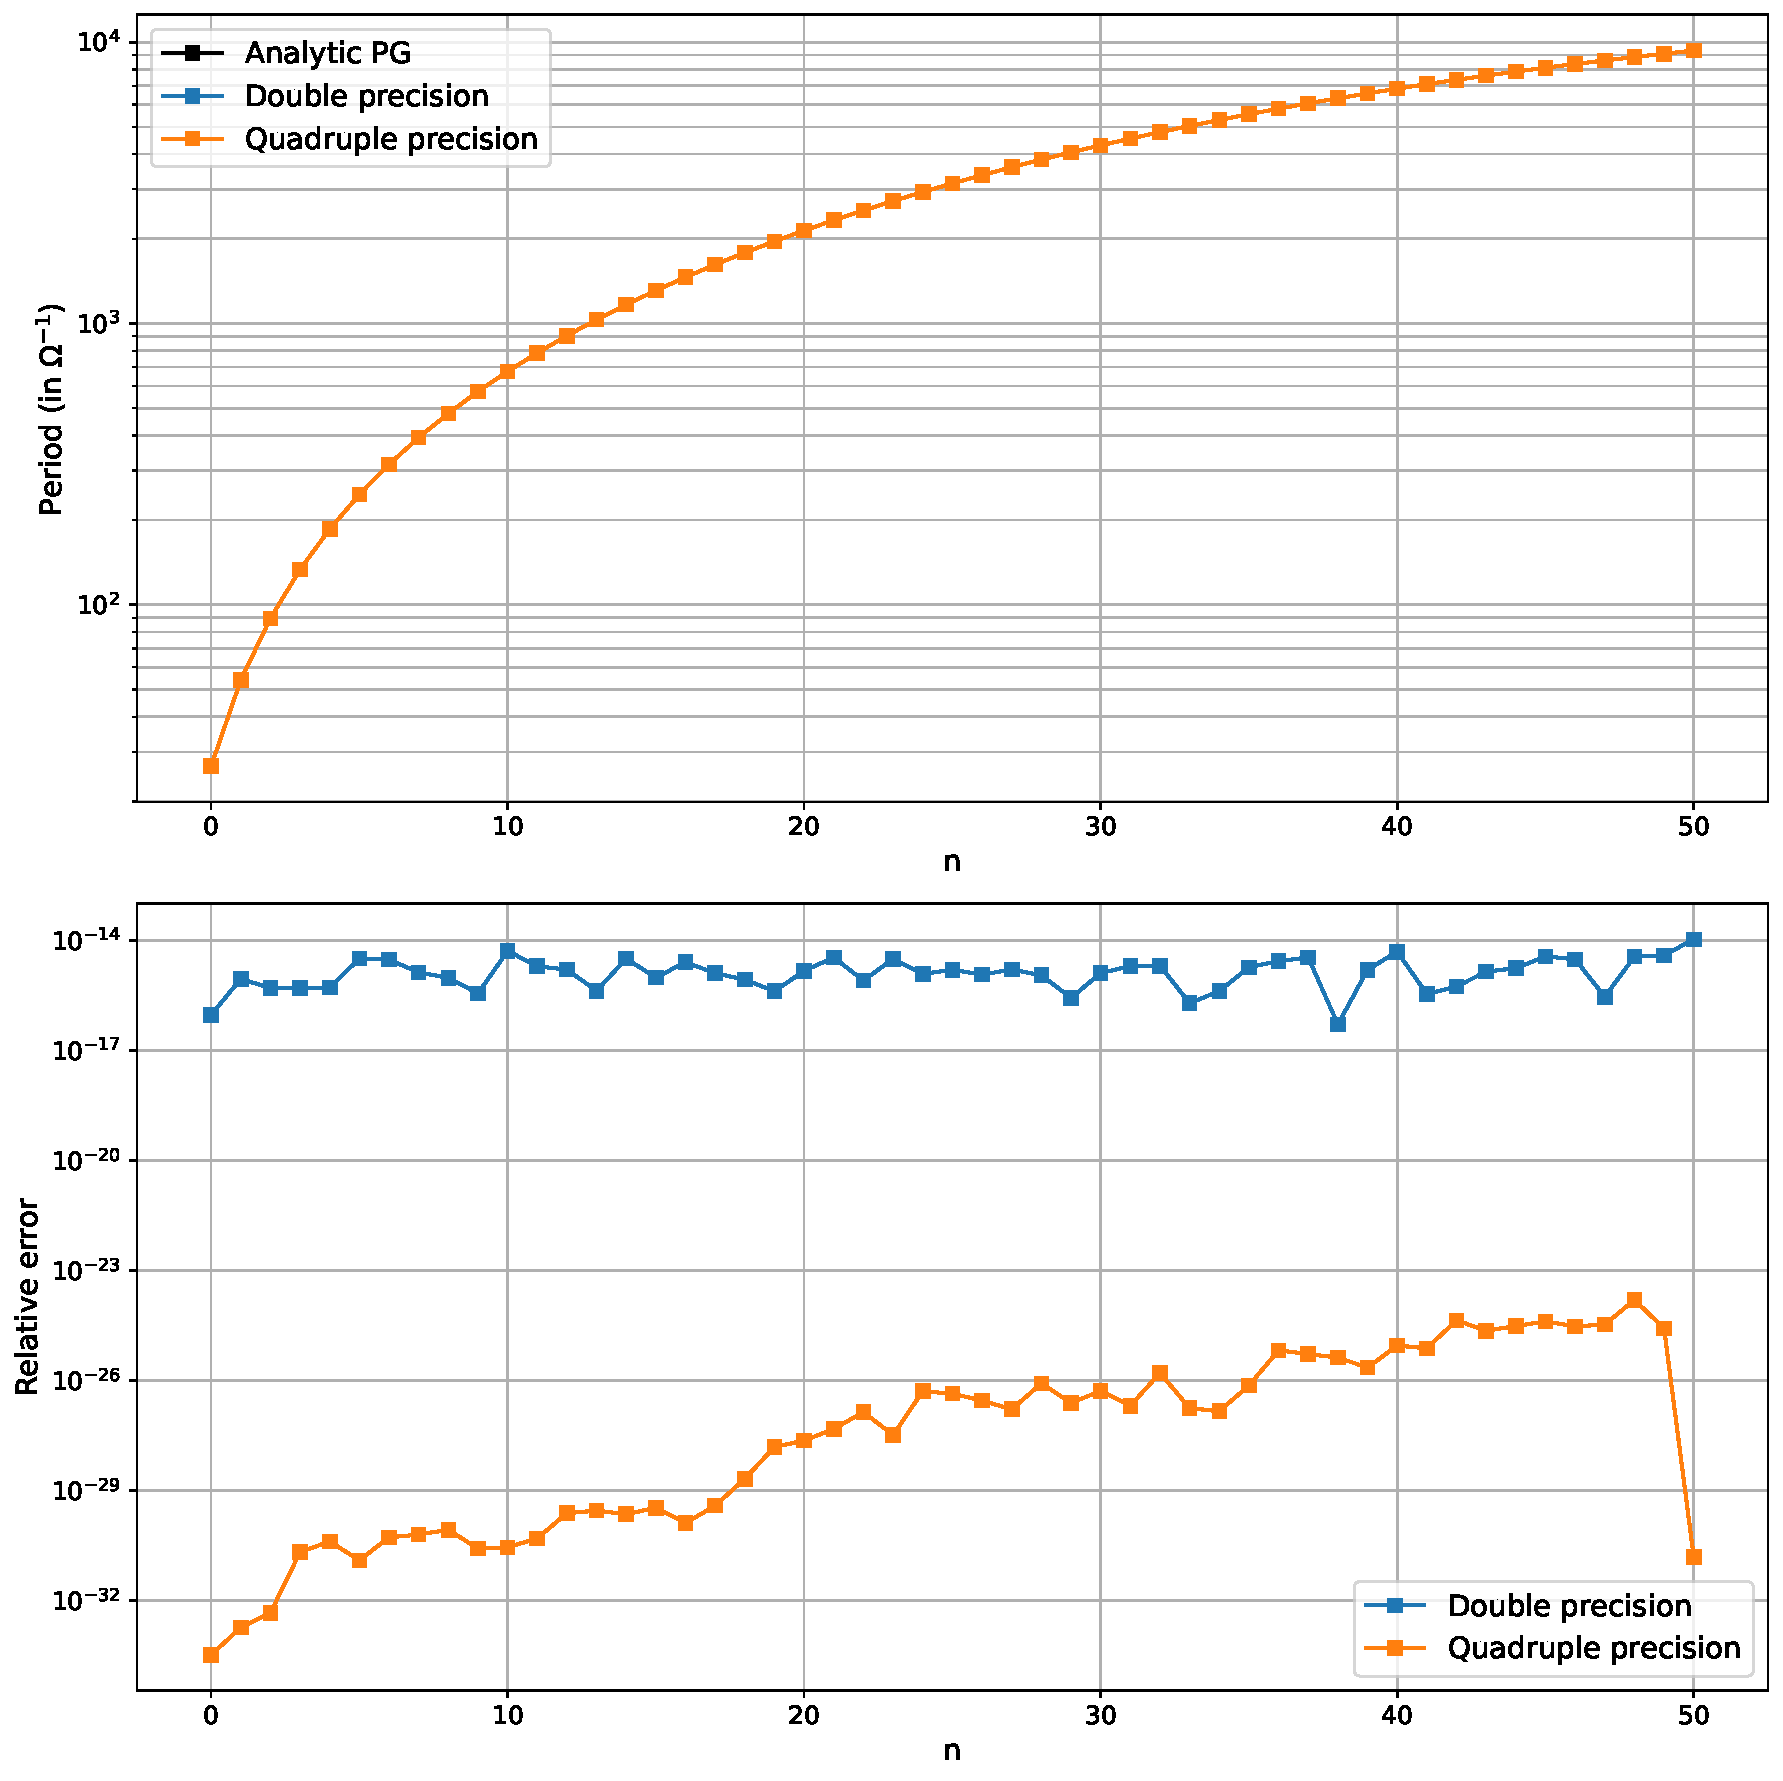
\includegraphics[width=.8\linewidth]{../../out/eigen/Malkus/Reduced/Analytical_error_precision_fast.pdf}
    \caption{Eigenperiods (upper panel) for $m=3$ fast modes under Malkus background field, solved to double precision and quadruple precision, with their respective errors from the analytical solution (lower panel). Both calculations are done using the reduced system and a truncation level $N=50$.}
\end{figure}

\begin{figure}[htbp]
    \centering
    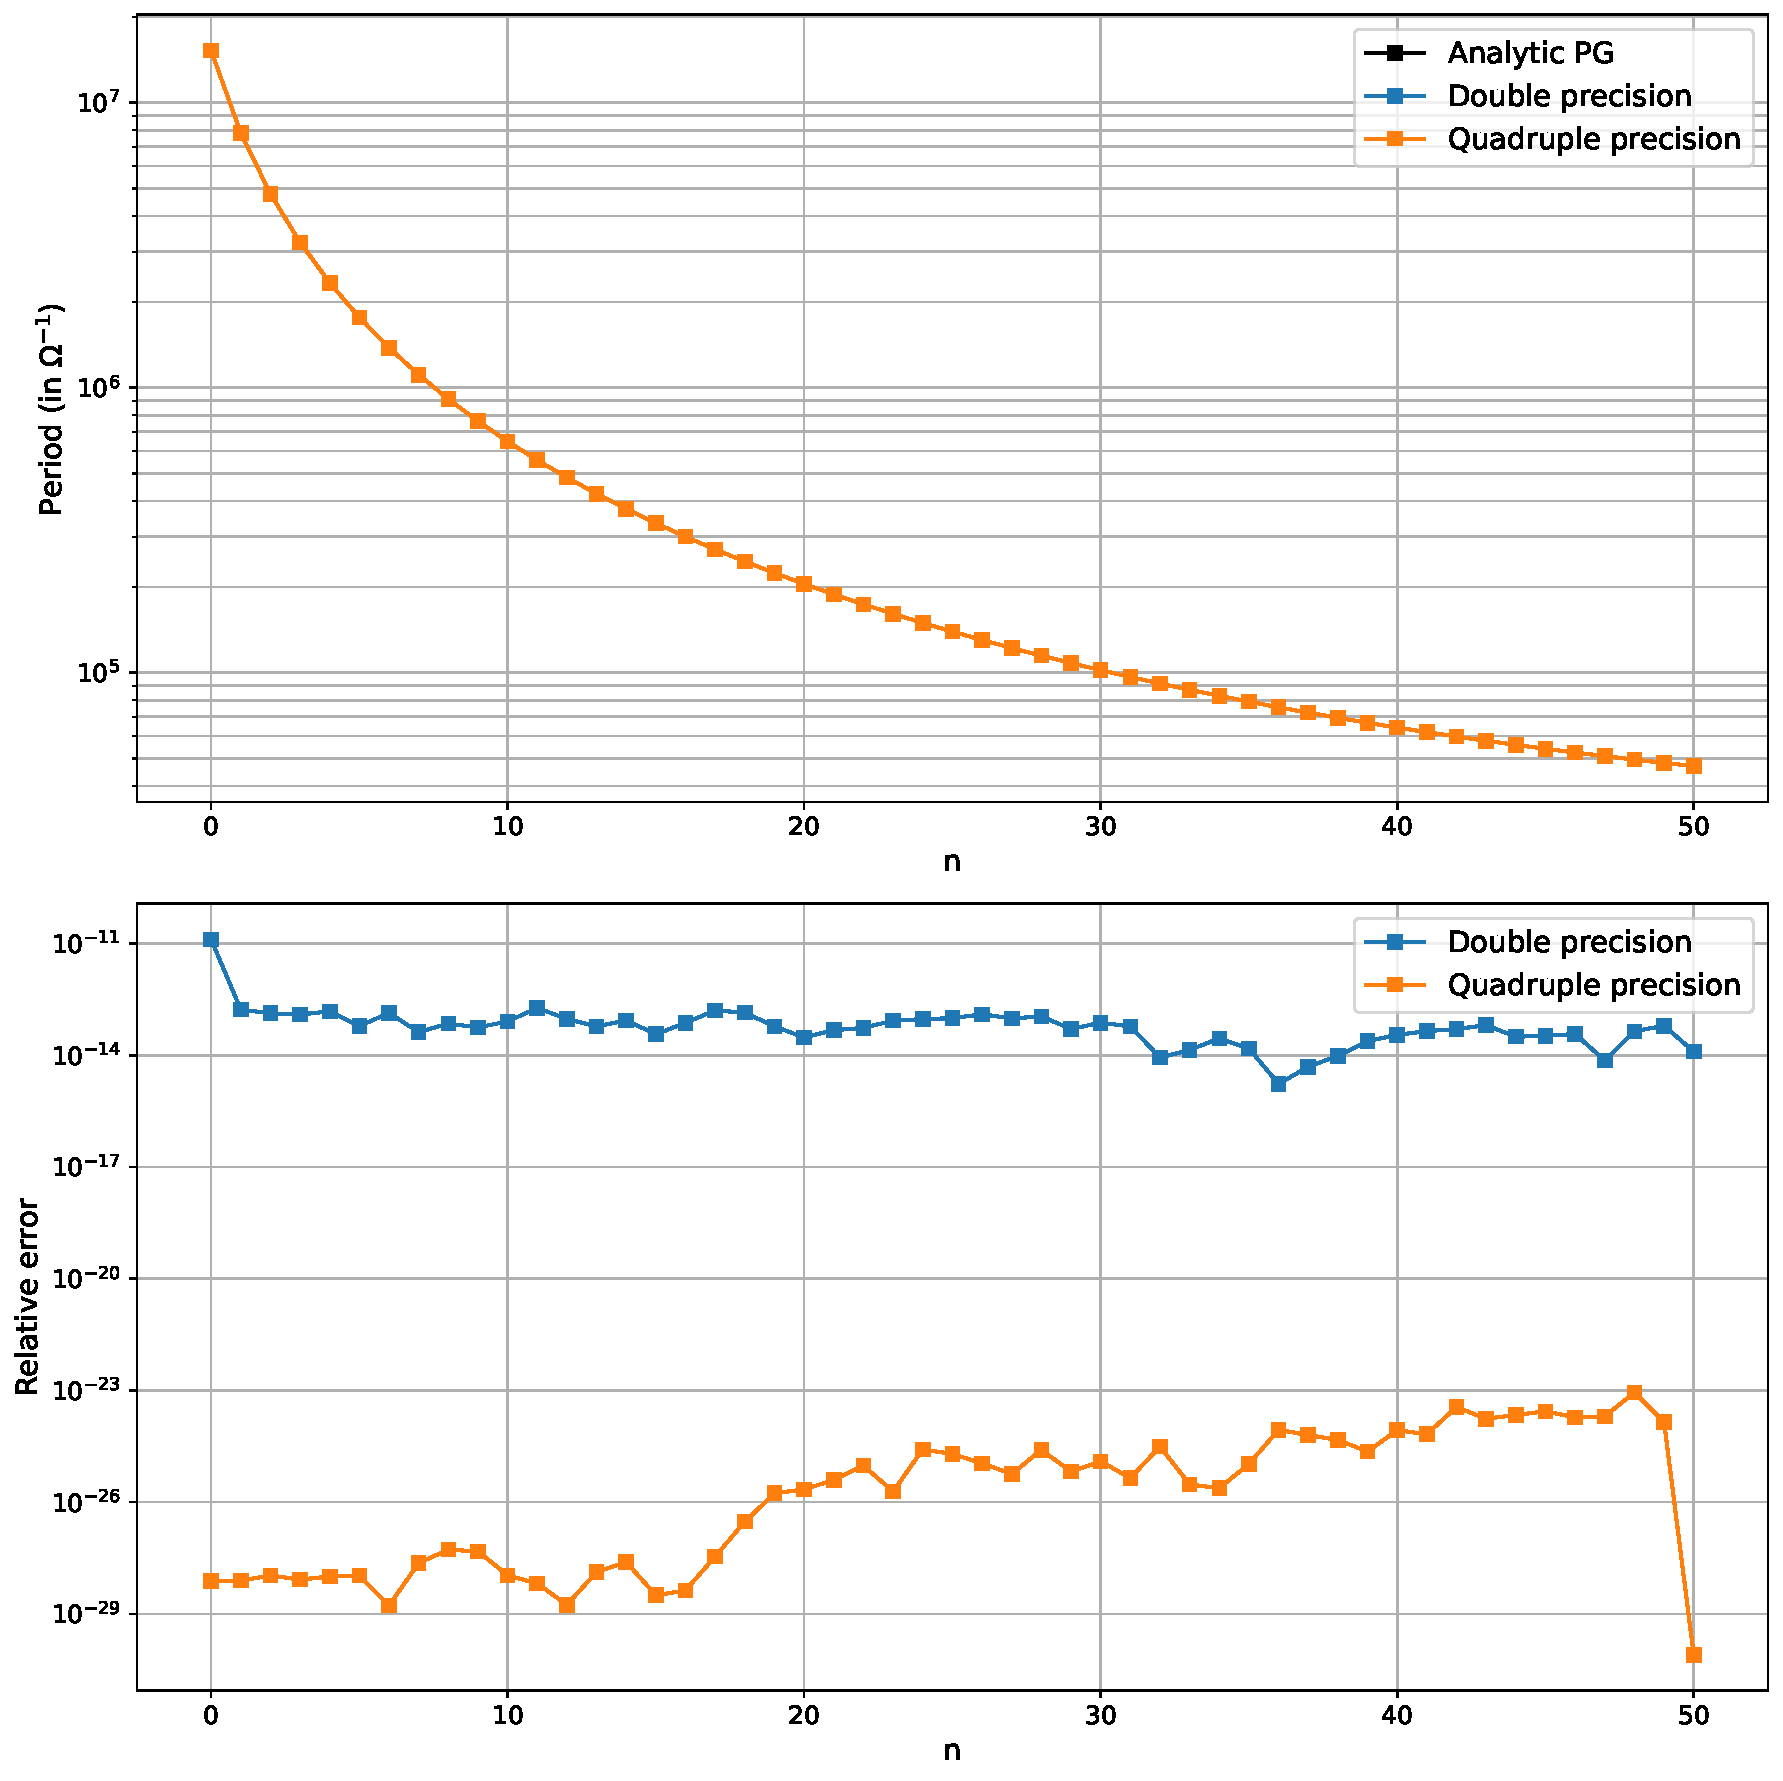
\includegraphics[width=.8\linewidth]{../../out/eigen/Malkus/Reduced/Analytical_error_precision_slow.pdf}
    \caption{Eigenperiods (upper panel) for $m=3$ slow modes under Malkus background field, solved to double precision and quadruple precision, with their respective errors from the analytical solution (lower panel). Both calculations are done using the reduced system and a truncation level $N=50$.}
\end{figure}



\section{Eigenvalue filtering}

Boyd's eigenvalue shift:
\begin{equation}
    \delta_j = \min_{k\in[1, N_2]} \frac{\left|\lambda_j(N_1) - \lambda_k(N_2)\right|}{\sigma_j}
\end{equation}

Maximum trailing rate of exponential convergence:
\begin{equation}
    C_j = \min_{n} \frac{\max_{k\geq n} \log\left|\frac{a_k^{(j)}}{a_n^{(j)}}\right|}{\left|n - n_0^{(j)}\right| + 1}
\end{equation}


\clearpage

\appendix

\chapter{Code design}

\section{Unifined Modelling Language (UML) graphs of the code}

\begin{figure}[ht]
    \centering
    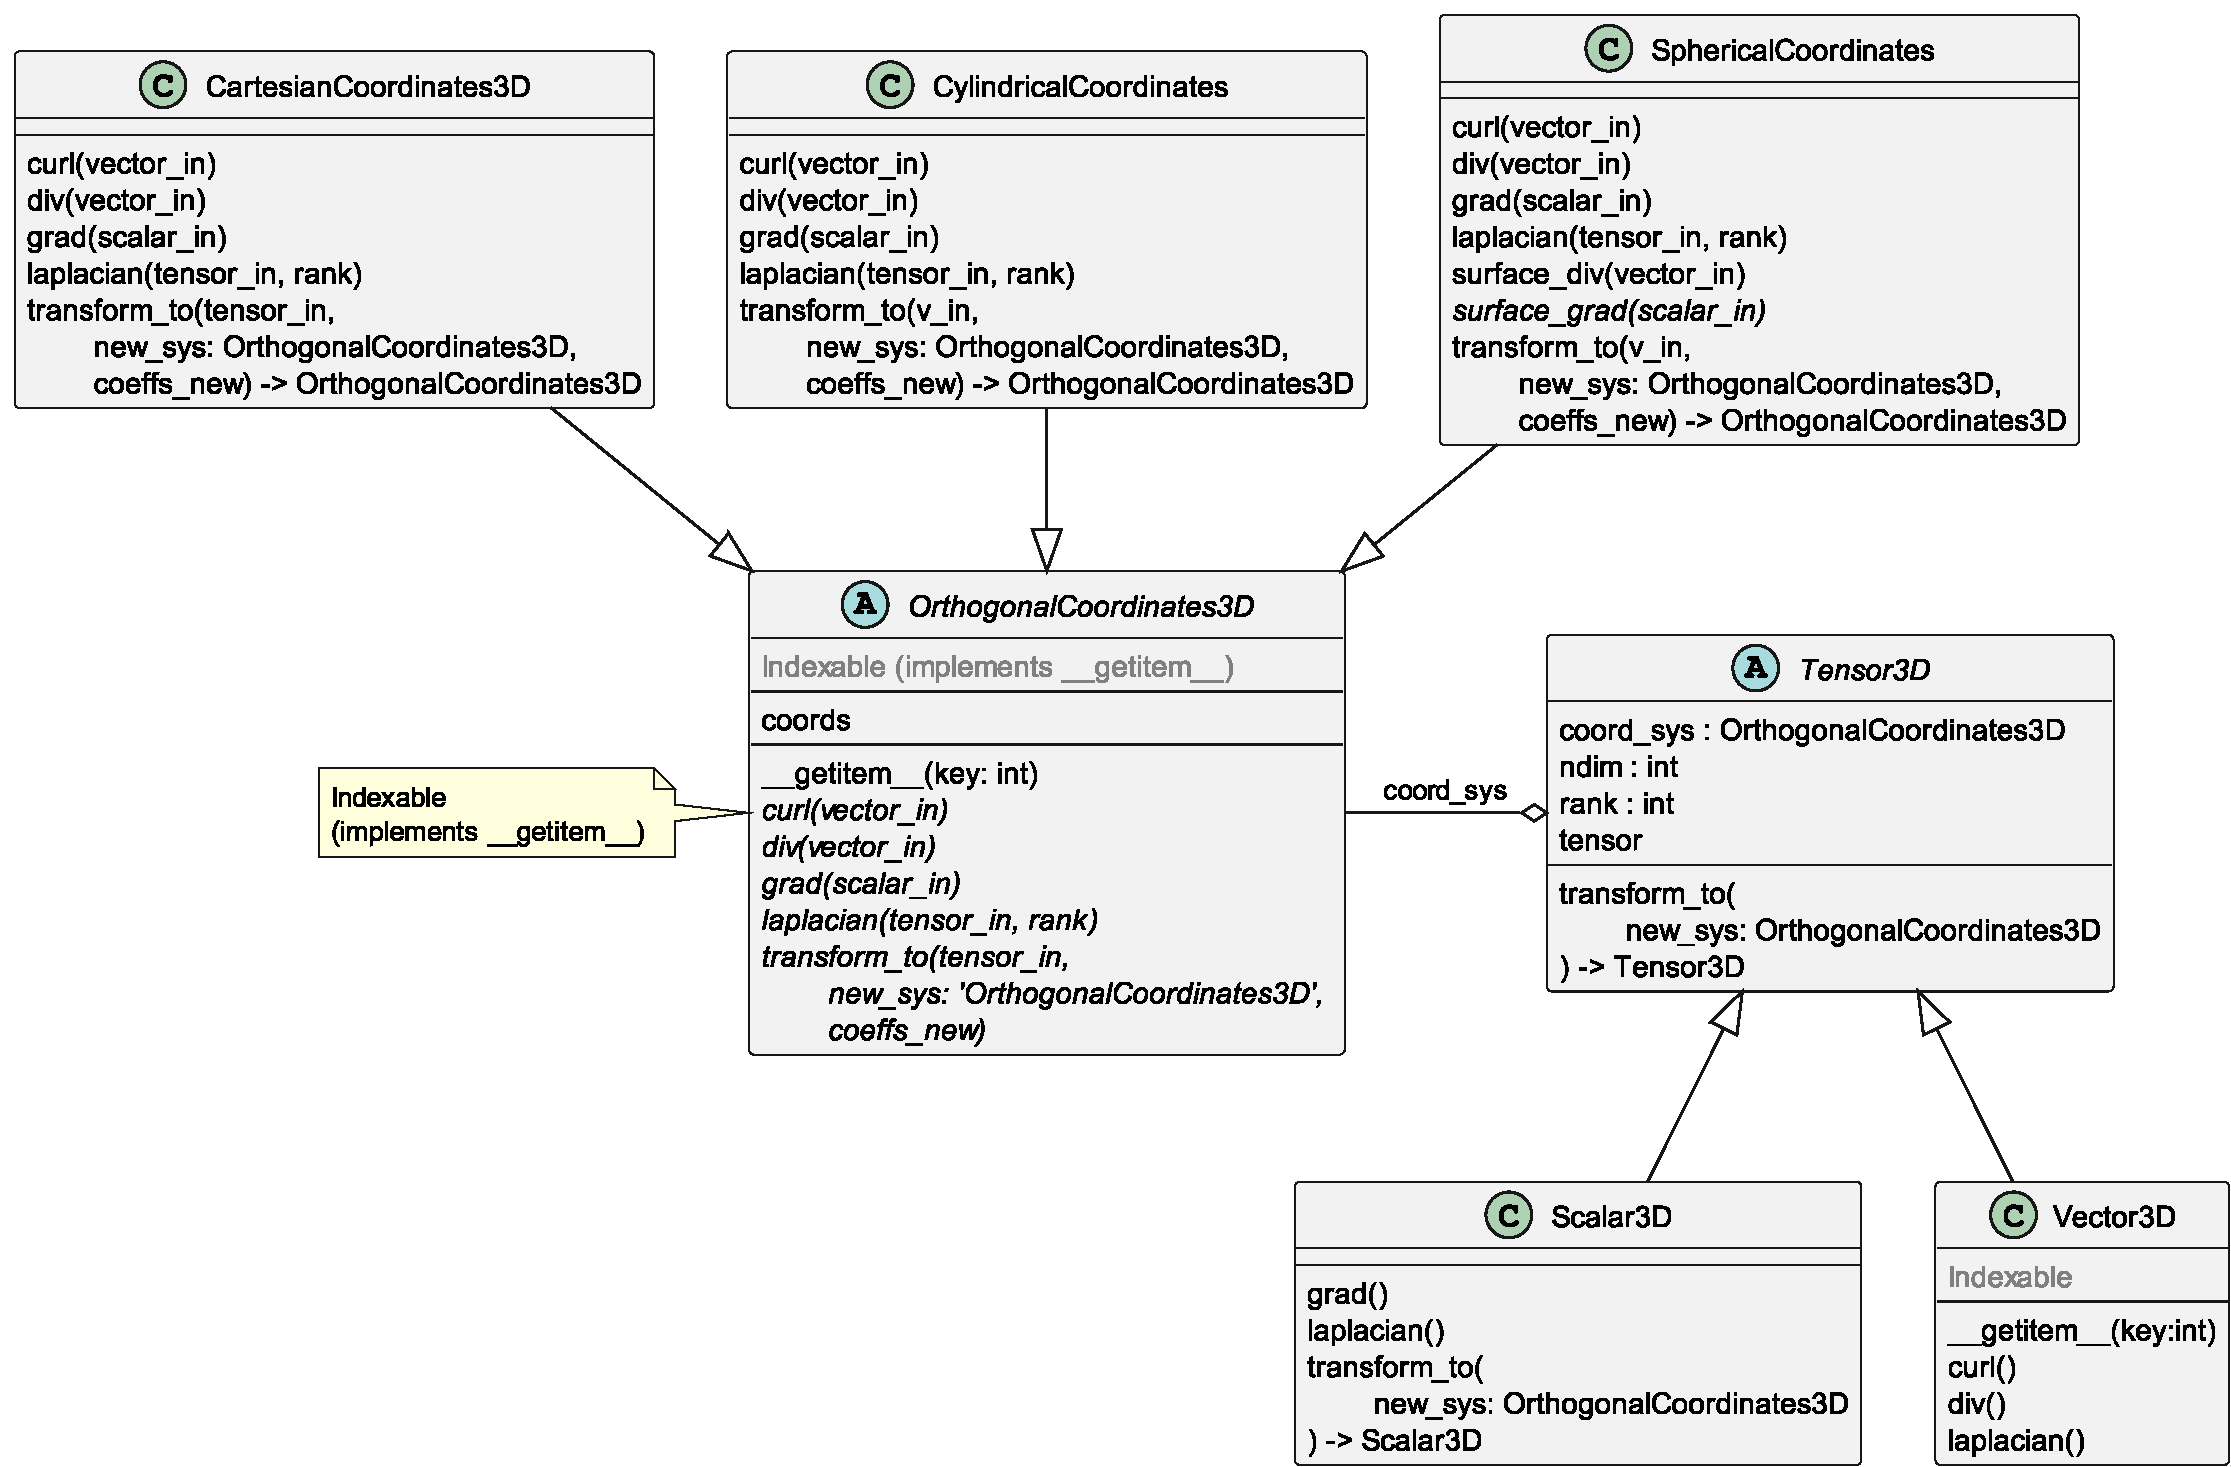
\includegraphics[width=\linewidth]{../Materials/classes_vector_calculus.pdf}
    \caption{Module for supplementary vector operations and calculus.}
\end{figure}


\begin{figure}[ht]
    \centering
    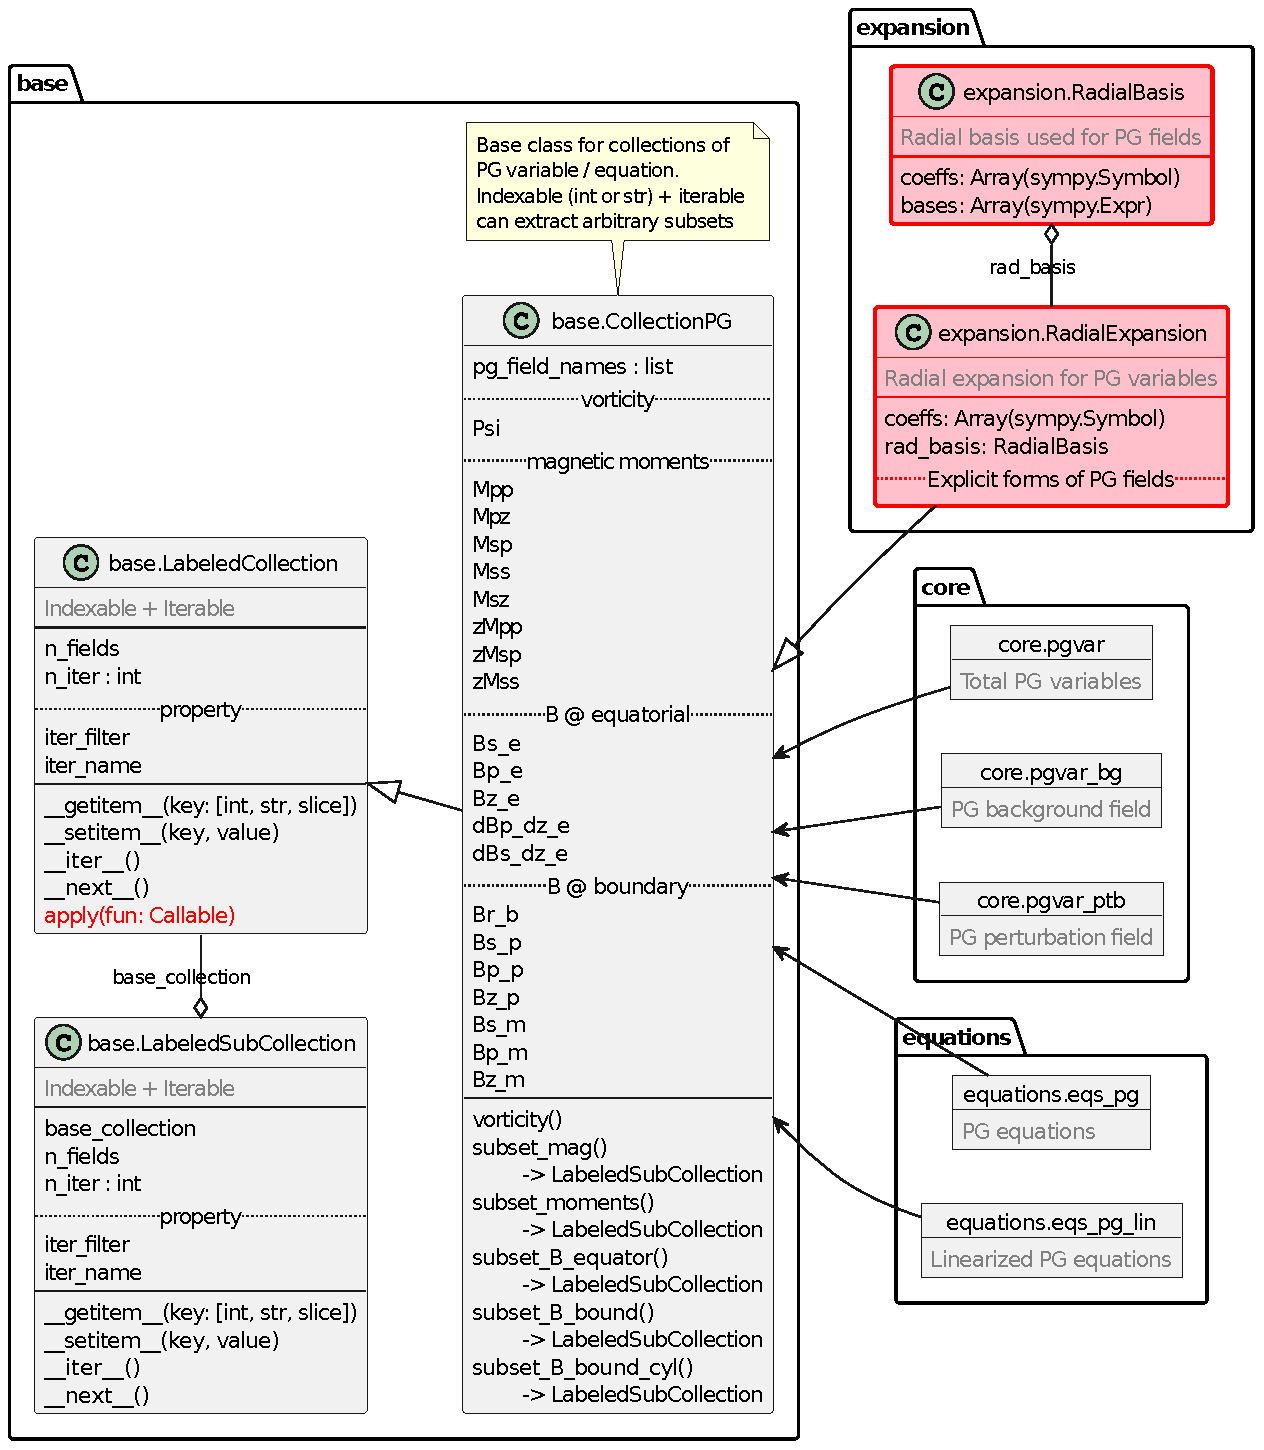
\includegraphics[width=\linewidth]{../Materials/classes_pg_model.pdf}
    \caption{Module PG model. Red items are items to be implemented}
\end{figure}


\clearpage

% [Deprecated][Archived] Derivation of regularity constraints on magnetic moments, following Daria's approach
% \section{Extended expansion for magnetic moments}

The three components of magnetic fields in cylindrical coordinates can be expanded as
\begin{equation}
\begin{aligned}
    B_s &= s g_0 + \sum_{m\neq 0} \left(\lambda_m s^{|m|-1} + g_m s^{|m|+1}\right) e^{im\phi}, \\ 
    B_\phi &= s h_0 + \sum_{m\neq 0} \left(i \sgn(m) \lambda_m s^{|m|-1} + h_m s^{|m|+1}\right) e^{im\phi}, \\ 
    B_z &= f_0 + \sum_{m\neq 0} f_m s^{|m|} e^{im\phi},
\end{aligned}
\end{equation}
where the regularity constraints from \textcite{lewis_physical_1990} is used. The coefficients are regular functions of $z$ and $s$, and according to symmetry arguments they are even functions of $s$. Therefore, the explicit dependency can be written as
\begin{equation}
    \lambda_m = \lambda_m(z),\quad g_m = g_m(z, s^2),\quad h_m = h_m(z, s^2),\quad f_m = f_m(z, s^2).
\end{equation}
Note for the quantities to be real, the Fourier coefficients should satisfy
\[
    \lambda_{-m}^* = \lambda_m,\quad g_{-m}^* = g_m,\quad h_{-m}^* = h_m,\quad f_{-m}^* = f_m.
\]
Here the asterik superscript $\cdot^*$ denotes complex conjugate. Of course, a corollary is that the zero-azimuthal-wavenumber terms, $g_0, h_0, f_0 \in \mathbb{R}$. Also, $(i \sgn(-m) \lambda_{-m})^* = i\sgn(m) \lambda_m$ is automatically satisified. Therefore, $c_m c_{-m} = c_m c_m^* = |c_m|^2$ for any coefficients.

\subsection{Magnetic moment $B_s^2$ rederived}

\begin{equation}
\begin{aligned}
    B_s^2 &= s^2 g_0^2 + 2s g_0 \sum_{m\neq 0} \left(\lambda_m s^{|m|-1} + g_m s^{|m|+1}\right) e^{im\phi} \\
    &\quad + \sum_{n,k\neq 0} \left(\lambda_n \lambda_k s^{|n|+|k|-2} + \left(\lambda_n g_k + g_n \lambda_k\right) s^{|n| + |k|} + g_n g_k s^{|n|+|k|+2} \right) e^{i(n+k)\phi} \\ 
    &= \left\{g_0^2 s^2 + \sum_{n\neq 0} \left[\lambda_n \lambda_{-n} s^{2|n|-2} + \left(\lambda_n g_{-n} + g_n \lambda_{-n}\right) s^{2|n|} + g_n g_{-n}  s^{2|n|+ 2} \right]\right\} \\ 
    &\quad + \sum_{m\neq 0} e^{im\phi} \Bigg\{2g_0 \lambda_m s^{|m|} + 2 g_0 g_m s^{|m|+2} \\
    &\qquad + \sum_{n\neq 0, m} \left[\lambda_n\lambda_{m-n} s^{|n|+|n-m|-2} + \left(\lambda_n g_{m-n} + g_n \lambda_{m-n}\right)s^{|n|+|n-m|} + g_n g_{m-n} s^{|n|+|n-m|+2}\right] \Bigg\}
    % &= \left\{ g_0^2 s^2 + \sum_{n\neq 0} \left[|\lambda_n|^2 s^{2|n|-2} + \left(\lambda_n \overline{g_n} + g_n \overline{\lambda_n}\right)s^{2|n|} + |g_n|^2 s^{2|n|+2}\right]\right\} + \sum_{m\neq 0} e^{im\phi} \Bigg\{ 2s^{|m|} \left(g_0 \lambda_m + g_0 g_m s^2\right)\\
    % &\qquad + \sum_{n\neq 0, m} \left[\lambda_n\lambda_{m-n} s^{|n|+|n-m|-2} + \left(\lambda_n g_{m-n} + g_n \lambda_{m-n}\right)s^{|n|+|n-m|} + g_n g_{m-n} s^{|n|+|n-m|+2}\right] \Bigg\}
\end{aligned}
\end{equation}
There is further simplification that can be performed on the final term. By dividing the nontrivial azimuthal wavenumbers into positive and negative branches, the contribution from the cross-terms is apparently written as
\begin{equation}
\begin{aligned}
    &\sum_{m > 0} e^{im\phi} \left[2 g_0 \lambda_m s^m + 2g_0 g_m s^{m+2}\right] + \sum_{m<0} e^{im\phi} \left[2 g_0 \lambda_m s^{-m} + 2g_0 g_m s^{-m+2}\right] \\ 
    =& \sum_{m > 0} e^{im\phi} \left[2 g_0 \lambda_m s^m + 2g_0 g_m s^{m+2}\right] +\sum_{m>0} e^{-im\phi} \left[2 g_0 \lambda_{-m} s^m + 2g_0 g_{-m} s^{m+2}\right] \\
    =& \sum_{m > 0} e^{im\phi} \left[2 g_0 \lambda_m s^m + 2g_0 g_m s^{m+2}\right] +\sum_{m>0} e^{-im\phi} \left[2 g_0 \lambda_m^* s^m + 2g_0 g_m^* s^{m+2}\right]
\end{aligned}
\end{equation}
For the second contribution, we can further separate the inner summation into three parts: the part where $n$ and $m-n$ have the same sign, the part where $n > 0$ and $m-n < 0$, and the part where $n < 0$ and $m-n > 0$. Let us consider the case when $m>0$ first.
\begin{equation}
\begin{aligned}
    &\sum_{n\neq 0, m} \left[\lambda_n\lambda_{m-n} s^{|n|+|n-m|-2} + \left(\lambda_n g_{m-n} + g_n \lambda_{m-n}\right)s^{|n|+|n-m|} + g_n g_{m-n} s^{|n|+|n-m|+2}\right] \\ 
    =& \left(\sum_{n < 0} + \sum_{0 < n < m} + \sum_{n > m}\right) \left[\lambda_n\lambda_{m-n} s^{|n|+|n-m|-2} + \left(\lambda_n g_{m-n} + g_n \lambda_{m-n}\right)s^{|n|+|n-m|} + g_n g_{m-n} s^{|n|+|n-m|+2}\right] \\ 
    =& \sum_{n < 0} \left[\lambda_n\lambda_{m-n} s^{m-2n-2} + \left(\lambda_n g_{m-n} + g_n \lambda_{m-n}\right)s^{m-2n} + g_n g_{m-n} s^{m-2n+2}\right] \\ 
    &+ \sum_{0<n<m} \left[\lambda_n\lambda_{m-n} s^{m-2} + \left(\lambda_n g_{m-n} + g_n \lambda_{m-n}\right)s^{m} + g_n g_{m-n} s^{m+2}\right] \\ 
    &+ \sum_{n > m} \left[\lambda_n\lambda_{m-n} s^{2n-m-2} + \left(\lambda_n g_{m-n} + g_n \lambda_{m-n}\right)s^{2n-m} + g_n g_{m-n} s^{2n-m+2}\right] \\ 
    =& \sum_{0<n<m} \left[\lambda_n\lambda_{m-n} s^{m-2} + \left(\lambda_n g_{m-n} + g_n \lambda_{m-n}\right)s^{m} + g_n g_{m-n} s^{m+2}\right] \\ 
    &+ \sum_{n > 0} \left[\lambda_{-n}\lambda_{m+n} s^{m+2n-2} + \left(\lambda_{-n} g_{m+n} + g_{-n} \lambda_{m+n}\right)s^{m+2n} + g_{-n} g_{m+n} s^{m+2n+2}\right] \\ 
    &+ \sum_{n > 0} \left[\lambda_{n+m}\lambda_{-n} s^{2n+m-2} + \left(\lambda_{n+m} g_{-n} + g_{n+m} \lambda_{-n}\right)s^{2n+m} + g_{n+m} g_{-n} s^{2n+m+2}\right] \\ 
    =& \sum_{0<n<m} \left[\lambda_n\lambda_{m-n} s^{m-2} + \left(\lambda_n g_{m-n} + g_n \lambda_{m-n}\right)s^{m} + g_n g_{m-n} s^{m+2}\right] \\ 
    &+ 2\sum_{n > 0} \left[\lambda_{n+m} \lambda_n^* s^{m+2n-2} + \left(\lambda_{n+m} g_n^* + g_{n+m} \lambda_n^*\right) s^{m+2n} + g_{n+m} g_n^* s^{m+2n+2}\right]
\end{aligned}
\end{equation}
The symmetry of $n$ and $m-n$ enables collapsing the two summations into one.
This way it is even possible to write explicitly the coefficient of $e^{im\phi}$ as an expansion of $s$. For $m > 0$, the Fourier coefficient for $B_s^2$ therefore reads
\begin{equation}
\begin{aligned}
    &s^{m-2} \sum_{0<n<m} \lambda_n \lambda_{m-n} + s^m \left(2g_0 \lambda_m + \sum_{0<n<m} (\lambda_n g_{m-n} + g_n \lambda_{m-n}) + 2 \lambda_{m+1} \lambda_1^*\right) \\ 
    +& s^{m+2} \left(2g_0 g_m + \sum_{0 < n < m} g_n g_{m-n} + 2 \left(\lambda_{m+2} \lambda_2^* + \lambda_{m+1} g_1^* + g_{m+1} \lambda_1^*\right) \right) \\
    +& \sum_{n > 1} s^{m+2n} \left[\lambda_{m+n+1} \lambda_{n+1}^* + \lambda_{m+n} g_n^* + g_{m+n} \lambda_n^* + g_{m+n-1} g_{n-1}^*\right].
\end{aligned}
\end{equation}
The situation for $m < 0$ is fairly similar, and can be straightforwardly obtained again using the complex conjugate property of the Fourier coefficients of real fields,
\begin{equation}
    \begin{aligned}
        &s^{|m|-2} \sum_{0<n<|m|} (\lambda_n \lambda_{|m|-n})^* + s^{|m|} \left(2g_0 \lambda_{|m|}^* + \sum_{0<n<|m|} ((\lambda_n g_{|m|-n})^* + (g_n \lambda_{|m|-n})^*) + 2 \lambda_{|m|+1}^* \lambda_1\right) \\ 
        +& s^{|m|+2} \left(2g_0 g_{|m|}^* + \sum_{0 < n < |m|} (g_n g_{|m|-n})^* + 2 \left(\lambda_{|m|+2}^* \lambda_2 + \lambda_{|m|+1}^* g_1 + g_{|m|+1}^* \lambda_1\right) \right) \\
        +& \sum_{n > 1} s^{|m|+2n} \left[\lambda_{|m|+n+1}^* \lambda_{n+1} + \lambda_{|m|+n}^* g_n + g_{|m|+n}^* \lambda_n + g_{|m|+n-1}^* g_{n-1}\right].
    \end{aligned}
\end{equation}
The full expansion can then be written in terms of the Fourier coefficients of $B_s$ as
\begin{equation}
\begin{aligned}
    B_s^2 &= \left\{2|\lambda_1|^2 + s^2\left(g_0^2 + 2|\lambda_2|^2 + 4 \Re[\lambda_1 g_1^*]\right) + 2\sum_{n>1} s^{2n} \left(|\lambda_{n+1}|^2 + |g_{n-1}|^2 + 2 \Re[\lambda_n g_n^*]\right)\right\} \\
    + \sum_{m>0} &e^{im\phi} \Bigg\{s^{m-2} \sum_{0<n<m} \lambda_n \lambda_{m-n} + s^m \left(2g_0 \lambda_m + \sum_{0<n<m} (\lambda_n g_{m-n} + g_n \lambda_{m-n}) + 2 \lambda_{m+1} \lambda_1^* \right) \\ 
    +& s^{m+2} \left(2g_0 g_m + \sum_{0 < n < m} g_n g_{m-n} + 2 \left(\lambda_{m+2} \lambda_2^* + \lambda_{m+1} g_1^* + g_{m+1} \lambda_1^*\right) \right) \\
    +& \sum_{n > 1} s^{m+2n} \left[\lambda_{m+n+1} \lambda_{n+1}^* + \lambda_{m+n} g_n^* + g_{m+n} \lambda_n^* + g_{m+n-1} g_{n-1}^* \right]\Bigg\} + \sum_{m<0} e^{im\phi} \left(\cdots\right).
\end{aligned}
\end{equation}
We therefore recover the asymptotic behaviour at $s=0$ for $B_s^2$,
\begin{equation}
\begin{aligned}
    \left(B_s^2\right)_{m=0} &= 2 |\lambda_1|^2 + O(s^2) \\ 
    \left(B_s^2\right)_{|m|=1} &= 2s \left(g_0 \lambda_1 + \lambda_{2} \lambda_1^*\right) e^{i\phi} + 2s \left(g_0 \lambda_1^* + \lambda_{2}^* \lambda_1\right) e^{-i\phi} + O(s^3) \\ 
    &= 2s \left[\left(2g_0 \lambda_1^R + \lambda_2^R \lambda_1^R + \lambda_2^I \lambda_1^I\right)\cos\phi - \left(2g_0 \lambda_1^I + \lambda_2^I \lambda_1^R - \lambda_2^R \lambda_1^I \right) \sin\phi\right] + O(s^3) \\
    \left(B_s^2\right)_{|m|>1} &= s^{|m|-2} \sum_{0 < n < |m|} \left(\lambda_n \lambda_{|m|-n} e^{i|m|\phi} + \lambda_n^* \lambda_{|m|-n}^* e^{-i|m|\phi}\right) + O\left(s^{|m|}\right) \\ 
    = s^{|m|-2} &\sum_{0 < n < |m|} \left[ \left(\lambda_n^R \lambda_{|m|-n}^R - \lambda_n^I \lambda_{|m|-n}^I\right) \cos (|m|\phi) - \left(\lambda_n^R \lambda_{|m|-n}^I + \lambda_n^I \lambda_{|m|-n}^R\right) \sin(|m|\phi)\right] + O(s^{|m|})
\end{aligned}
\end{equation}
Apart from a prefactor, this is the same as in \textcite{holdenried-chernoff_long_2021} for $|m|\neq 1$. For $|m|=1$, the contribution from the cross-term $g_0$ seems to be missing in Daria's dissertation. The summation $\sum_{n+k=m}$ (in \cite{holdenried-chernoff_long_2021}) is also misleading; it should technically be constrained to positive $n$ and $k$, so the summation is actually not an infinite sum. That being said, the leading order behaviour in $s$ is correct. The later analysis on the integral in $z$ is also not affected by this discrepancy.

\subsection{General Fourier expansion formulae for moments}

Let two vector components be expressed by
\[
    B_a = s a_0^+ + \sum_{m\neq 0} e^{im\phi} \left(a_m^- s^{|m|-1} + a_m^+ s^{|m|+1} \right),\quad
    B_b = s b_0^+ + \sum_{m\neq 0} e^{im\phi} \left(b_m^- s^{|m|-1} + b_m^+ s^{|m|+1} \right)
\]
The expression applies to either of the two horizontal components of the magnetic fields in cylindrical coordinates. Using the same method, without assuming the complex conjugate property of the Fourier coefficients, we can write
\begin{equation}
\begin{aligned}
    B_a B_b =& \bigg\{\left(a_1^- b_{-1}^- + a_{-1}^- b_1^-\right) + s^2 \left[a_0^+ b_0^+ + \left(a_2^- b_{-2}^- + a_{-2}^- b_2^-\right) + \left(a_1^- b_{-1}^+ + a_{1}^+ b_{-1}^- + a_{-1}^- b_{1}^+ + a_{-1}^+ b_1^-\right)\right]\\
    + \sum_{n > 1}& s^{2n} \left[\left(a_{n+1}^- b_{-n-1}^- + a_{-n-1}^- b_{n+1}^-\right) + \left(a_n^- b_{-n}^+ + a_{n}^+ b_{-n}^- + a_{-n}^- b_{n}^+ + a_{-n}^+ b_n^-\right) + \left(a_{n-1}^+ b_{1-n}^+ + a_{1-n}^+ b_{n-1}^+\right) \right]\bigg\} \\ 
    +\sum_{m > 0} e^{im\phi}& \Bigg\{ s^{m-2} \sum_{0\leq n\leq m} a_n^- b_{m-n}^- + s^m \left[a_{-1}^- b_{m+1}^- + a_{m+1}^- b_{-1}^- + \sum_{0\leq n\leq m} \left(a_n^- b_{m-n}^+ + a_n^+ b_{m-n}^-\right)\right] \\
    + s^{m+2}& \left[a_{-2}^- b_{m+2}^- + a_{m+2}^- b_{-2}^- + a_{m+1}^- b_{-1}^+ + a_{m+1}^+ b_{-1}^- + a_{-1}^+ b_{m+1}^- + a_{-1}^- b_{m+1}^+ + \sum_{0\leq n\leq m} a_n^+ b_{m-n}^+ \right] \\
    + s^m& \sum_{n \geq 2} s^{2n} \bigg[\left(a_{-n-1}^- b_{m+n+1}^- + a_{m+n+1}^- b_{-n-1}^-\right) + \left(a_{-n}^{-} b_{m+n}^+ + a_{-n}^{+} b_{m+n}^- + a_{m+n}^{-} b_{-n}^+ + a_{m+n}^{+} b_{-n}^-\right) \\
    &\quad + \left(a_{-n+1}^+b_{m+n-1}^+ + a_{-n+1}^{-} b_{m+n-1}^+\right)\bigg] \Bigg\} \\ 
    +\sum_{m < 0} e^{im\phi}& \Bigg\{ s^{|m|-2} \sum_{m\leq n\leq 0} a_n^- b_{m-n}^- + s^{|m|} \left[a_{1}^- b_{m-1}^- + a_{m-1}^- b_{1}^- + \sum_{m\leq n\leq 0} \left(a_n^- b_{m-n}^+ + a_n^+ b_{m-n}^-\right)\right] \\
    + s^{|m|+2}& \left[a_{2}^- b_{m-2}^- + a_{m-2}^- b_{2}^- + a_{m-1}^- b_{1}^+ + a_{m-1}^+ b_{1}^- + a_{1}^+ b_{m-1}^- + a_{1}^- b_{m-1}^+ + \sum_{m\leq n\leq 0} a_n^+ b_{m-n}^+ \right] \\
    + s^{|m|} & \sum_{n \geq 2} s^{2n} \bigg[\left(a_{n+1}^- b_{m-n-1}^- + a_{m-n-1}^- b_{n+1}^-\right) + \left(a_{n}^{-} b_{m-n}^+ + a_{n}^{+} b_{m-n}^- + a_{m-n}^{-} b_{n}^+ + a_{m-n}^{+} b_{n}^-\right) \\
    &\quad + \left(a_{n-1}^+b_{m-n+1}^+ + a_{n-1}^{-} b_{m-n+1}^+\right)\bigg] \Bigg\}
\end{aligned}
\end{equation}
Here we already used the property $a_0^- = b_0^- = 0$ to add trivial terms, and merged cross terms involving $a_0^+$, $b_0^+$ in the summation $\sum_{0\leq n \leq m}$ or $\sum_{m\leq n \leq 0}$. Plugging in $a_{n}^- = b_n^- = \lambda_n$ and $a_n^+ = b_n^+ = g_n$, and assuming $\lambda_{-n}^* = \lambda_n$, $g_{-n}^* = g_n$, one can easily verify that the equation leads to the expansion for $B_s^2$. The lowest order term in $s$ for arbitrary Fourier coefficient is also readily given as a corollary:
\begin{equation}
\begin{aligned}
    \left(B_a B_b\right)_{m=0} &= a_1^- b_{-1}^- + a_{-1}^- b_{1}^- + O\left(s^2\right) \\ 
    \left(B_a B_b\right)_{|m|=1} &= s e^{+i\phi}\left[a_{-1}^- b_{2}^- + a_{2}^- b_{-1}^- + a_1^- b_0^+ + a_0^+ b_1^-\right]\\
    &+ s e^{-i\phi}\left[a_{1}^- b_{-2}^- + a_{-2}^- b_{1}^- + a_{-1}^- b_0^+ + a_0^+ b_{-1}^-\right] + O\left(s^3\right) \\ 
    \left(B_a B_b\right)_{|m|>1} &= s^{|m|-2} e^{+i|m|\phi} \sum_{0\leq n \leq |m|} a_n^- b_{|m|-n}^- \\
    &+ s^{|m|-2} e^{-i|m|\phi} \sum_{-|m| \leq n \leq 0} a_n^- b_{-|m|-n}^- + O\left(s^{|m|}\right)
\end{aligned}
\end{equation}
On the other hand, a scalar that is regular in cylindrical coordinates takes the form
\begin{equation}
F = \sum_{m\in \mathbb{Z}} f_m s^{|m|} e^{im\phi} = f_0 + \sum_{m\neq 0} f_m s^{|m|} e^{im\phi}
\end{equation}
This applies to $B_z$. Its moment with any equatorial component takes the form
\begin{equation}
\begin{aligned}
    F B_a &= s f_0 a_0^+ + \sum_{n\neq 0} \left(f_{-n} a_n^- s^{2|n|-1} + f_{-n} a_n^+ s^{2|n|+1}\right) + \sum_{m\neq 0} \left[f_0 a_{m}^- s^{|m|-1} + \left(f_0 a_m^+ + f_m a_0^+\right) s^{|m|+1}\right] e^{im\phi} \\
    &+ \sum_{m > 0} e^{im\phi} \Bigg[s^{m-1} \sum_{0<n<m} f_{m-n} a_n^- + s^{m+1} \sum_{0<n<m} f_{m-n} a_n^+ \\
    &+\quad  \sum_{n>0} \left(\left(f_{-n} a_{m+n}^- + f_{m+n} a_{-n}^- \right) s^{m+2n-1} + \left(f_{-n} a_{m+n}^+ + f_{m+n} a_{-n}^+ \right) s^{m+2n+1} \right) \Bigg] \\
    &+ \sum_{m < 0} e^{im\phi} \Bigg[s^{|m|-1} \sum_{m<n<0} f_{m-n} a_n^- + s^{m+1} \sum_{m<n<0} f_{m-n} a_n^+ \\
    &+\quad  \sum_{n>0} \left(\left(f_{n} a_{m-n}^- + f_{m-n} a_{n}^- \right) s^{|m|+2n-1} + \left(f_{n} a_{m-n}^+ + f_{m-n} a_{n}^+ \right) s^{|m|+2n+1} \right) \Bigg] \\
    F B_a &= s \left(f_0 a_0^+ + f_{-1} a_1^- + f_1 a_{-1}^-\right) + \sum_{n\geq 1} s^{2n+1} \left(f_{-n-1} a_{n+1}^- + f_{n+1} a_{-n-1}^- + f_{-n} a_n^+ + f_n a_{-n}^+ \right) \\
    &+ \sum_{m > 0} e^{im\phi} s^{m-1} \Bigg[ \left(\sum_{0\leq n\leq m} f_{m-n} a_n^-\right) + \left(\sum_{0\leq n\leq m} f_{m-n} a_n^+ + f_{-1}a_{m+1}^- + f_{m+1} a_{-1}^- \right) s^2 \\
    &\qquad + \sum_{n\geq 2} s^{2n} \left(f_{-n} a_{m+n}^- + f_{m+n} a_{-n}^- + f_{1-n} a_{m+n-1}^+ + f_{m+n-1} a_{1-n}^+\right) \Bigg] \\ 
    &+ \sum_{m < 0} e^{im\phi} s^{|m|-1} \Bigg[ \left(\sum_{m\leq n\leq 0} f_{m-n} a_n^-\right) + \left(\sum_{m\leq n\leq 0} f_{m-n} a_n^+ + f_{1}a_{m-1}^- + f_{m-1} a_{1}^- \right) s^2 \\
    &\qquad + \sum_{n\geq 2} s^{2n} \left(f_{n} a_{m-n}^- + f_{m-n} a_{n}^- + f_{n-1} a_{m-n+1}^+ + f_{m-n+1} a_{n-1}^+\right) \Bigg]
\end{aligned}
\end{equation}
The lowest order behaviour in $s$ at different azimuthal wavenumber:
\begin{equation}
\begin{aligned}
    (FB_a)_{m=0} &= s \left(f_0 a_0^+ + f_{-1} a_1^- + f_1 a_{-1}^-\right) + O(s^3) \\ 
    (FB_a)_{m\neq 0} &= s^{|m|-1} \sum_{0\leq n \leq |m|} \left( f_{|m|-n} a_n^- e^{i|m|\phi} + f_{-|m|+n} a_{-n}^- e^{-i|m|\phi}\right) + O(s^{|m|+1}).
\end{aligned}
\end{equation}

\subsection{Axial asymptotic of magnetic moments}

Here I write out the explicit form of the lowest order dependency on $s$ at different azimuthal wavenumber for magnetic moments. For $B_s^2$, we have $a_m^- = b_m^- = \lambda_m$, and $a_m^+ = b_m^+ = g_m$. The asymptotics at $s\rightarrow 0$ are as follows, which have already been derived in the first section:
\begin{equation}
\begin{aligned}
    \left(B_s^2\right)_{m=0} &= 2(\lambda_1 \lambda_{-1}) + O\left(s^2\right) \\ 
    \left(B_s^2\right)_{|m|=1} &= 2 s \left[\left(\lambda_2 \lambda_{-1} + g_0 \lambda_1\right) e^{i\phi} + \left(\lambda_{-2} \lambda_{1} + g_0 \lambda_{-1}\right) e^{-i\phi}\right] + O\left(s^3\right) \\ 
    \left(B_s^2\right)_{|m|>1} &= s^{|m|-2} \left[e^{i|m|\phi} \sum_{0\leq n \leq |m|} \lambda_n \lambda_{|m|-n} + e^{-i|m|\phi} \sum_{-|m|\leq n\leq 0} \lambda_n \lambda_{-|m|-n}\right] + O\left(s^{|m|}\right).
\end{aligned}
\end{equation}
Note that here I didn't assume the complex conjugate property between the positive and the negative wavenumbers. For $B_\phi^2$, we have $a_m^- = b_m^- = i\sgn(m)\lambda_m$, and $a_m^+ = b_m^+ = h_m$. We see that the product $a_m^- b_n^- = \lambda_m \lambda_n$ if $m$ and $n$ have different signs, but $-\lambda_m \lambda_n$ if $m$ and $n$ have the same signs. The asymptotics are then given by
\begin{equation}
    \begin{aligned}
        \left(B_\phi^2\right)_{m=0} &= 2 (\lambda_1 \lambda_{-1}) + O\left(s^2\right) \\ 
        \left(B_\phi^2\right)_{|m|=1} &= 2 s \left[\left(\lambda_2 \lambda_{-1} + i h_0 \lambda_1\right) e^{i\phi} + \left(\lambda_{-2} \lambda_{1} - i h_0 \lambda_{-1}\right) e^{-i\phi}\right] + O\left(s^3\right) \\ 
        \left(B_\phi^2\right)_{|m|>1} &= -s^{|m|-2} \left[e^{i|m|\phi} \sum_{0\leq n \leq |m|} \lambda_n \lambda_{|m|-n} + e^{-i|m|\phi} \sum_{-|m|\leq n\leq 0} \lambda_n \lambda_{-|m|-n}\right] + O\left(s^{|m|}\right).
\end{aligned}
\end{equation}
We see that these expressions already differ from those in \textcite{holdenried-chernoff_long_2021}. These include: a two prefactor difference (present in \cite{holdenried-chernoff_long_2021}, but not here) in $|m| > 1$; summation difference in $|m| > 1$; missing terms for $|m|=1$; and missing imaginary unit for one part of $|m|=1$. Nevertheless, the conclusions seem to be correct: lowest-order $s$-dependencies for $B_s^2$ and $B_\phi^2$ are coupled in $m=0$ and $|m|>1$, with prefactor $+1$ and $-1$, respectively. The coupling is not seen for $|m|=1$.

For $B_s B_\phi$, we plug in $a_m^- = \lambda_m$, $b_m^- = i\sgn(m) \lambda_m$, $a_m^+ = g_m$ and $b_m^+ = h_m$. The asymptotics
\begin{equation}
    \begin{aligned}
        \left(B_s B_\phi\right)_{m=0} &= (-i\lambda_1 \lambda_{-1} + i\lambda_{-1} \lambda_1) + O\left(s^2\right) = O\left(s^2\right) \\ 
        \left(B_s B_\phi\right)_{|m|=1} &= s \left[\left(h_0 \lambda_1 + i g_0 \lambda_1\right) e^{i\phi} + \left(h_0 \lambda_{-1} - i g_0 \lambda_{-1}\right) e^{-i\phi}\right] + O\left(s^3\right) \\ 
        \left(B_s B_\phi\right)_{|m|>1} &= i s^{|m|-2} \left[e^{i|m|\phi} \sum_{0\leq n \leq |m|} \lambda_n \lambda_{|m|-n} - e^{-i|m|\phi} \sum_{-|m|\leq n\leq 0} \lambda_n \lambda_{-|m|-n}\right] + O\left(s^{|m|}\right).
    \end{aligned}
\end{equation}
Thus this moment is coupled to $B_s^2$ and $B_\phi^2$ by a factor $i\sgn(m)$ and $-i\sgn(m)$, respectively. Similar couplings are not apprent for $m=0$ and $|m|=1$.

In the moments $B_z B_s$ and $B_z B_\phi$, $B_z$ is treated as scalar, and we need to use the formula involving one equatorial component and one scalar. Taking $a_{m}^- = \lambda_m$ and $a_m^+ = g_m$, we have 
\begin{equation}
\begin{aligned}
    \left(B_z B_s\right)_{m=0} &= s \left(f_0 g_0 + f_{-1} \lambda_1 + f_1 \lambda_{-1}\right) \\ 
    \left(B_z B_s\right)_{m\neq 0} &= s^{|m|-1} \sum_{0\leq n\leq |m|}\left(f_{|m|-n} \lambda_n e^{i|m|\phi} + f_{-|m|+n} \lambda_{-n} e^{-i|m|\phi}\right) + O\left(s^{|m|+1}\right)
\end{aligned}
\end{equation}
Taking $a_m^- = i\sgn(m)\lambda_m$ and $a_m^+ = h_m$, we have
\begin{equation}
    \begin{aligned}
        \left(B_z B_s\right)_{m=0} &= s \left(f_0 h_0 + i f_{-1} \lambda_1 - i f_1 \lambda_{-1}\right) \\ 
        \left(B_z B_s\right)_{m\neq 0} &= s^{|m|-1} \sum_{0\leq n\leq |m|}\left(i f_{|m|-n} \lambda_n e^{i|m|\phi} - i f_{-|m|+n} \lambda_{-n} e^{-i|m|\phi}\right) + O\left(s^{|m|+1}\right)
    \end{aligned}
\end{equation}
Thus these two moment are coupled in the lowest order of $s$ in $m\neq 0$ by a factor $i\sgn(m)$, while there is probably no such coupling in $m=0$. We can conclude that despite all the discrepancies in intermediate steps, the coupling between the moments are the same between this derivation and \textcite{holdenried-chernoff_long_2021}.

\subsection{Axial integral of moment of Fourier coefficients}

It is unsurprising that the Fourier coefficients for $B_s^2$ (and easily shown for all moments) are always summation of $c_n c_k$, where $c=f, g, h, \lambda$. In other words, \textbf{the Fourier coefficients for the magnetic moments are summations of moments of the Fourier coefficients for the magnetic fields.} In fact, I can write the magnetic moment in the general form
\[
    B_a B_b = \sum_m e^{im\phi} s^{m + \Delta_m^{a,b}} \sum_{k \geq 0} s^{2k} \left(\sum_{p,q\in S_{m,k}} c_p c_q\right).
\]
where $\Delta_m^{a,b}$ determines the correction to the lowest order of $s$ at azimuthal wavenumber $m$ (\textcite{holdenried-chernoff_long_2021} found a more concise expression: $s^{||m|-1|})$, given components $a$ and $b$, and $S_{m,k}$ gives the set of all coefficient pairs to sum over at given azimuthal wavenumber $m$ and radial degree index $k$. Among all these terms, however, the only terms with dependency on $z$ are $c_p c_q$. It follows that the axial integrals are
\[
    \overline{z^n B_a B_b} = \sum_m e^{im\phi} s^{m + \Delta} \sum_{k \geq 0} s^{2k} \sum_{p,q} \overline{z^n c_p c_q},\quad
    \widetilde{z^n B_a B_b} = \sum_m e^{im\phi} s^{m + \Delta} \sum_{k \geq 0} s^{2k} \sum_{p,q} \widetilde{z^n c_p c_q}.
\]
If expanding the coefficients in power series of $z$, 
\[
    c_n (z) = \sum_{p \geq 0} c_n^p z^p
\]
the symmetric axial integral of the moments of coefficients are given by
\begin{equation}
\begin{aligned}
    \overline{z^n c_a c_b} &= \int_{-H}^H z^n c_a c_b \, dz = \sum_{p, q \geq 0} c_a^p c_b^q \int_{-H}^H z^{p + q + n} \, dz \\
    &= \sum_{p,q} c_a^p c_b^q \frac{H^{p+q+n+1} - (-H)^{p+q+n+1}}{p + q + n + 1} 
    = \sum_{k\geq 0} \frac{2H^{2k+1}}{2k+1} \sum_{0\leq p \leq 2k-n} c_m^p c_n^{2k-n-p} \\ 
    &= \sqrt{1-s^2} \sum_{k\geq 0} \frac{2}{2k+1} \sum_{0\leq p \leq 2k-n} c_a^p c_b^{2k-n-p} \left(1-s^2\right)^k \\
    &= 2 \sqrt{1-s^2} \sum_{k\geq \lceil \frac{n}{2} \rceil} \frac{\left(c_a^{p} * c_b^p\right)_{2k-n}}{2k+1} \left(1 - s^2\right)^k \\ 
    &= 2 \left(1 - s^2\right)^{\lceil \frac{n}{2} \rceil + \frac{1}{2}} \sum_{k\geq 0} \frac{\left(c_a^{p} * c_b^p\right)_{2k+2\lceil \frac{n}{2} \rceil-n}}{2k+2\lceil\frac{n}{2}\rceil + 1} \left(1 - s^2\right)^k
\end{aligned}
\end{equation}
where $(c_a^p * c_b^p)_{k} = \sum_{0\leq p \leq k} c_a^p c_b^{k-p}$ is the k-th element of the (non-circular) convolution of the finite-length sequence $c_a^p$ and $c_b^p$, $p=0:k$. The only terms left in the integrands are the even powers of $z$. Similarly, the anti-symmetric axial integral is
\begin{equation}
    \begin{aligned}
        \widetilde{z^n c_a c_b} &= \int_{-H}^H \sgn(z) z^n c_a c_b \, dz = \sum_{p, q \geq 0} c_a^p c_b^q \int_{-H}^H \sgn(z) z^{p + q + n} \, dz \\
        &= \sum_{p,q} c_a^p c_b^q \frac{H^{p+q+n+1} + (-H)^{p+q+n+1}}{p + q + n + 1} 
        = \sum_{k\geq 0} \frac{2H^{2k+2}}{2k+2} \sum_{0\leq p \leq 2k+1-n} c_a^p c_b^{2k+1-n-p} \\ 
        &= \sum_{k\geq 0} \frac{1}{k+1} \sum_{0\leq p \leq 2k+1-n} c_a^p c_b^{2k+1-n-p} \left(1-s^2\right)^{k+1} \\
        &= \left(1 - s^2\right) \sum_{k\geq \lceil \frac{n-1}{2}\rceil} \frac{\left(c_a^{p} * c_b^p\right)_{2k+1-n}}{k+1} \left(1 - s^2\right)^k \\ 
        &= \left(1 - s^2\right)^{\lceil \frac{n+1}{2}\rceil} \sum_{k\geq 0} \frac{\left(c_a^{p} * c_b^p\right)_{2k+1+2\lceil \frac{n-1}{2} \rceil -n}}{k+\lceil \frac{n+1}{2}\rceil} \left(1 - s^2\right)^k
    \end{aligned}
\end{equation}
Plugging $n=0$ in the symmetric integral, and $n=0,1$ in the anti-symmetric integral respectively. The symmetric and anti-symmetric integrals of coefficient moments in the symmetric and anti-symmetric integrals of magnetic moments read
\begin{equation}
    \begin{aligned}
        \overline{c_a c_b} &= \left(1 - s^2\right)^{\frac{1}{2}} \sum_{k \geq 0} \frac{2(c_a^p * c_b^p)_{2k}}{2k+1} \left(1 - s^2\right)^k = \left(1 - s^2\right)^{\frac{1}{2}} \left[\sum_{k\geq 0} \frac{2(c_a^p * c_b^p)_{2k}}{2k+1} + O\left(s^2\right)\right], \\ 
        \widetilde{c_a c_b} &= \left(1 - s^2\right) \sum_{k \geq 0} \frac{(c_a^p * c_b^p)_{2k+1}}{k+1} \left(1 - s^2\right)^k = \left(1 - s^2\right) \left[\sum_{k\geq 0} \frac{(c_a^p*c_b^p)_{2k+1}}{k+1} + O\left(s^2\right) \right], \\ 
        \widetilde{z c_a c_b} &= \left(1 - s^2\right) \sum_{k \geq 0} \frac{(c_a^p * c_b^p)_{2k}}{k+1} \left(1 - s^2\right)^k = \left(1 - s^2\right) \left[\sum_{k \geq 0} \frac{(c_a^p * c_b^p)_{2k}}{k+1} + O\left(s^2\right)\right].
    \end{aligned}
\end{equation}
Note that some coefficients (e.g. $g_m$, $h_m$ and $f_m$) are also functions of $s^2$. In these cases, the coefficients that are relevant in the leading order are the 0th-order coefficients in the power series of $s^2$, which will be written as $c_m^{p0}$. 

\subsection{Axial asymptotic of integrated moments}

With these formulae, we can derive the lowest order term in $s$ for the integrated $B_s^2$:
\begin{equation}
    \begin{aligned}
        \overline{B_s^2}_{m=0} &= 2 \overline{\lambda_1 \lambda_{-1}} + O\left(\overline{c_a c_b} s^2\right) = 2\left(1 - s^2\right)^{\frac{1}{2}} \left[\sum_{k\geq 0} \frac{2 (\lambda_1^p * \lambda_{-1}^p)_{2k}}{2k+1} + O\left(s^2\right)\right] \\ 
        \overline{B_s^2}_{|m|=1} &= 2 s \left(1 - s^2\right)^{\frac{1}{2}} \left[\sum_{k\geq 0} \frac{2}{2k+1} \left((\lambda_2^p * \lambda_{-1}^p)_{2k} + (g_0^{p0} * \lambda_{1}^p)_{2k}\right) + O\left(s^2\right)\right] e^{+i\phi} \\ 
        &+ 2 s \left(1 - s^2\right)^{\frac{1}{2}} \left[\sum_{k\geq 0} \frac{2}{2k+1} \left((\lambda_{-2}^p * \lambda_{1}^p)_{2k} + (g_0^{p0} * \lambda_{-1}^p)_{2k}\right) + O\left(s^2\right)\right] e^{-i\phi} \\
        \overline{B_s^2}_{|m|>1} &= s^{|m|-2} \left(1 - s^2\right)^{\frac{1}{2}} \left[\sum_{0\leq n \leq m} \sum_{k\geq 0} \frac{2(\lambda_n^p * \lambda_{|m|-n}^p)_{2k}}{2k+1} + O\left(s^2\right)\right] e^{+i|m|\phi} \\ 
        &+ s^{|m|-2} \left(1 - s^2\right)^{\frac{1}{2}} \left[\sum_{-|m|\leq n \leq 0} \sum_{k\geq 0} \frac{2(\lambda_n^p * \lambda_{-|m|-n}^p)_{2k}}{2k+1} + O\left(s^2\right)\right] e^{-i|m|\phi} \\
        &= s^{|m|-2} \left(1 - s^2\right)^{\frac{1}{2}} \left[\sum_{k\geq 0} \frac{2(\lambda_n^p * \lambda_{n}^p)_{0\leq n \leq |m|}^{0\leq p \leq 2k}}{2k+1} + O\left(s^2\right)\right] e^{+i|m|\phi} \\ 
        &+ s^{|m|-2} \left(1 - s^2\right)^{\frac{1}{2}} \left[\sum_{k\geq 0} \frac{2(\lambda_n^p * \lambda_{n}^p)_{-|m|\leq n \leq 0}^{0\leq p \leq 2k}}{2k+1} + O\left(s^2\right)\right] e^{-i|m|\phi}
    \end{aligned}
\end{equation}
where $(a_n^p * b_n^p)_{n\in S_n}^{p \in S_b}$ denotes the 2-D convolution on the 2-D sequences $a_n^p$ and $b_n^p$. It can be considered an example of more generalized convolution theorem, as $a_n^p$ can be considered the transform of the original field into the spectral domain, with Fourier basis in the azimuthal direction, and monomial basis in the $s$ and $z$ direction. Since moments are the products of fields, their spectral coefficients naturally consist of convolutions of spectral coefficients of the respective fields. The $\lambda_n^p * \lambda_n^p$ present here is the 2D "auto-convolution" of 2-D coefficients $\lambda_n^p$. Similarly, $\overline{B_\phi^2}$ has
\begin{equation}
    \begin{aligned}
        \overline{B_\phi^2}_{m=0} &= 2\left(1 - s^2\right)^{\frac{1}{2}} \left[\sum_{k\geq 0} \frac{2 (\lambda_1^p * \lambda_{-1}^p)_{2k}}{2k+1} + O\left(s^2\right)\right] \\ 
        \overline{B_\phi^2}_{|m|=1} &= 2 s \left(1 - s^2\right)^{\frac{1}{2}} \left[\sum_{k\geq 0} \frac{2}{2k+1} \left((\lambda_2^p * \lambda_{-1}^p)_{2k} + i (h_0^{p0} * \lambda_{1}^p)_{2k}\right) + O\left(s^2\right)\right] e^{+i\phi} \\ 
        &+ 2 s \left(1 - s^2\right)^{\frac{1}{2}} \left[\sum_{k\geq 0} \frac{2}{2k+1} \left((\lambda_{-2}^p * \lambda_{1}^p)_{2k} - i(h_0^{p0} * \lambda_{-1}^p)_{2k}\right) + O\left(s^2\right)\right] e^{-i\phi} \\
        \overline{B_\phi^2}_{|m|>1} &= -s^{|m|-2} \left(1 - s^2\right)^{\frac{1}{2}} \left[\sum_{k\geq 0} \frac{2(\lambda_n^p * \lambda_{n}^p)_{0\leq n \leq |m|}^{0\leq p \leq 2k}}{2k+1} + O\left(s^2\right)\right] e^{+i|m|\phi} \\ 
        &- s^{|m|-2} \left(1 - s^2\right)^{\frac{1}{2}} \left[\sum_{k\geq 0} \frac{2(\lambda_n^p * \lambda_{n}^p)_{-|m|\leq n \leq 0}^{0\leq p \leq 2k}}{2k+1} + O\left(s^2\right)\right] e^{-i|m|\phi}
    \end{aligned}
\end{equation}
and $\overline{B_s B_\phi}$ has
\begin{equation}
\begin{aligned}
    \overline{B_s B_\phi}_{m=0} &= \left(1 - s^2\right)^{\frac{1}{2}} O\left(s^2\right) \\ 
    \overline{B_s B_\phi}_{|m|=1} &= s \left(1 - s^2\right)^{\frac{1}{2}} \left[\sum_{k\geq 0} \frac{2((h_0^{p0} + ig_0^{p0}) * \lambda_{1}^p)_{2k}}{2k+1} + O\left(s^2\right)\right] e^{+i\phi} \\ 
    &+ s \left(1 - s^2\right)^{\frac{1}{2}} \left[\sum_{k\geq 0} \frac{2((h_0^{p0} - ig_0^{p0}) * \lambda_{-1}^p)_{2k}}{2k+1} + O\left(s^2\right)\right] e^{-i\phi} \\
    \overline{B_s B_\phi}_{|m|>1} &= i s^{|m|-2} \left(1 - s^2\right)^{\frac{1}{2}} \left[\sum_{k\geq 0} \frac{2(\lambda_n^p * \lambda_{n}^p)_{0\leq n \leq |m|}^{0\leq p \leq 2k}}{2k+1} + O\left(s^2\right)\right] e^{+i|m|\phi} \\ 
    &- is^{|m|-2} \left(1 - s^2\right)^{\frac{1}{2}} \left[\sum_{k\geq 0} \frac{2(\lambda_n^p * \lambda_{n}^p)_{-|m|\leq n \leq 0}^{0\leq p \leq 2k}}{2k+1} + O\left(s^2\right)\right] e^{-i|m|\phi}
\end{aligned}
\end{equation}
The Fourier coefficients of the five anti-symmetric integrals of moments take the form
\begin{equation}
\begin{aligned}
    \widetilde{B_z B_s}_{m=0} &= s \left(1 - s^2\right) \sum_{k\geq 0}\frac{1}{k+1}\left[(f_0^{p0}*g_0^{p0})_{2k+1} + (f_{-1}^{p0} * \lambda_{1}^p)_{2k+1} + (f_{1}^{p0} * \lambda_{-1}^p)_{2k+1} + O\left(s^2\right)\right] \\ 
    \widetilde{B_z B_s}_{m\neq 0} &= s^{|m|-1} \left(1 - s^2\right) \left[\sum_{k\geq 0} \frac{(f_n^{p0} * \lambda_n^p)_{0\leq n \leq |m|}^{0\leq p \leq 2k+1}}{k+1} + O\left(s^2\right)\right] e^{+i|m|\phi} \\ 
    &+ s^{|m|-1} \left(1 - s^2\right) \left[\sum_{k\geq 0} \frac{(f_n^{p0} * \lambda_n^p)_{-|m| \leq n \leq 0}^{0\leq p \leq 2k+1}}{k+1} + O\left(s^2\right)\right] e^{-i|m|\phi} \\ 
    \widetilde{B_z B_\phi}_{m=0} &= s \left(1 - s^2\right) \sum_{k\geq 0}\frac{1}{k+1}\left[(f_0^{p0}*h_0^{p0})_{2k+1} + i(f_{-1}^{p0} * \lambda_{1}^p)_{2k+1} - i(f_{1}^{p0} * \lambda_{-1}^p)_{2k+1} + O\left(s^2\right)\right] \\ 
    \widetilde{B_z B_\phi}_{m\neq 0} &= i s^{|m|-1} \left(1 - s^2\right) \left[\sum_{k\geq 0} \frac{(f_n^{p0} * \lambda_n^p)_{0\leq n \leq |m|}^{0\leq p \leq 2k+1}}{k+1} + O\left(s^2\right)\right] e^{+i|m|\phi} \\ 
    &-i s^{|m|-1} \left(1 - s^2\right) \left[\sum_{k\geq 0} \frac{(f_n^{p0} * \lambda_n^p)_{-|m| \leq n \leq 0}^{0\leq p \leq 2k+1}}{k+1} + O\left(s^2\right)\right] e^{-i|m|\phi}
\end{aligned}
\end{equation}
And the quantities with $z$ factors,
\begin{equation}
    \begin{aligned}
        \widetilde{zB_s^2}_{m=0} &= 2\left(1 - s^2\right) \left[\sum_{k\geq 0} \frac{(\lambda_1^p * \lambda_{-1}^p)_{2k}}{k+1} + O\left(s^2\right)\right] \\ 
        \widetilde{zB_s^2}_{|m|=1} &= 2 s \left(1 - s^2\right) \left[\sum_{k\geq 0} \frac{1}{k+1} \left((\lambda_2^p * \lambda_{-1}^p)_{2k} + (g_0^{p0} * \lambda_{1}^p)_{2k}\right) + O\left(s^2\right)\right] e^{+i\phi} \\ 
        &+ 2 s \left(1 - s^2\right) \left[\sum_{k\geq 0} \frac{1}{k+1} \left((\lambda_{-2}^p * \lambda_{1}^p)_{2k} + (g_0^{p0} * \lambda_{-1}^p)_{2k}\right) + O\left(s^2\right)\right] e^{-i\phi} \\
        \widetilde{zB_s^2}_{|m|>1} &= s^{|m|-2} \left(1 - s^2\right) \left[\sum_{k\geq 0} \frac{(\lambda_n^p * \lambda_{n}^p)_{0\leq n \leq |m|}^{0\leq p \leq 2k}}{k+1} + O\left(s^2\right)\right] e^{+i|m|\phi} \\ 
        &+ s^{|m|-2} \left(1 - s^2\right) \left[\sum_{k\geq 0} \frac{(\lambda_n^p * \lambda_{n}^p)_{-|m|\leq n \leq 0}^{0\leq p \leq 2k}}{k+1} + O\left(s^2\right)\right] e^{-i|m|\phi}
    \end{aligned}
\end{equation}
\begin{equation}
    \begin{aligned}
        \widetilde{zB_\phi^2}_{m=0} &= 2\left(1 - s^2\right) \left[\sum_{k\geq 0} \frac{(\lambda_1^p * \lambda_{-1}^p)_{2k}}{k+1} + O\left(s^2\right)\right] \\ 
        \widetilde{zB_\phi^2}_{|m|=1} &= 2 s \left(1 - s^2\right) \left[\sum_{k\geq 0} \frac{1}{k+1} \left((\lambda_2^p * \lambda_{-1}^p)_{2k} + i (h_0^{p0} * \lambda_{1}^p)_{2k}\right) + O\left(s^2\right)\right] e^{+i\phi} \\ 
        &+ 2 s \left(1 - s^2\right) \left[\sum_{k\geq 0} \frac{1}{k+1} \left((\lambda_{-2}^p * \lambda_{1}^p)_{2k} - i(h_0^{p0} * \lambda_{-1}^p)_{2k}\right) + O\left(s^2\right)\right] e^{-i\phi} \\
        \widetilde{zB_\phi^2}_{|m|>1} &= -s^{|m|-2} \left(1 - s^2\right) \left[\sum_{k\geq 0} \frac{(\lambda_n^p * \lambda_{n}^p)_{0\leq n \leq |m|}^{0\leq p \leq 2k}}{k+1} + O\left(s^2\right)\right] e^{+i|m|\phi} \\ 
        &- s^{|m|-2} \left(1 - s^2\right) \left[\sum_{k\geq 0} \frac{(\lambda_n^p * \lambda_{n}^p)_{-|m|\leq n \leq 0}^{0\leq p \leq 2k}}{k+1} + O\left(s^2\right)\right] e^{-i|m|\phi}
    \end{aligned}
\end{equation}
\begin{equation}
    \begin{aligned}
        \widetilde{zB_s B_\phi}_{m=0} &= \left(1 - s^2\right) O\left(s^2\right) \\ 
        \widetilde{zB_s B_\phi}_{|m|=1} &= s \left(1 - s^2\right) \left[\sum_{k\geq 0} \frac{((h_0^{p0} + ig_0^{p0}) * \lambda_{1}^p)_{2k}}{k+1} + O\left(s^2\right)\right] e^{+i\phi} \\ 
        &+ s \left(1 - s^2\right) \left[\sum_{k\geq 0} \frac{((h_0^{p0} - ig_0^{p0}) * \lambda_{-1}^p)_{2k}}{k+1} + O\left(s^2\right)\right] e^{-i\phi} \\
        \widetilde{zB_s B_\phi}_{|m|>1} &= i s^{|m|-2} \left(1 - s^2\right) \left[\sum_{k\geq 0} \frac{(\lambda_n^p * \lambda_{n}^p)_{0\leq n \leq |m|}^{0\leq p \leq 2k}}{k+1} + O\left(s^2\right)\right] e^{+i|m|\phi} \\ 
        &- is^{|m|-2} \left(1 - s^2\right) \left[\sum_{k\geq 0} \frac{(\lambda_n^p * \lambda_{n}^p)_{-|m|\leq n \leq 0}^{0\leq p \leq 2k}}{k+1} + O\left(s^2\right)\right] e^{-i|m|\phi}
    \end{aligned}
\end{equation}


\subsection{Regularity constraints}

Similar to \textcite{holdenried-chernoff_long_2021}, we can conclude some constraints that the moments or the fields have to satisfy if the underlying fields fulfill regularity constraints according to \textcite{lewis_physical_1990}. We notice that the relevant fields can be expressed as
\[
\Phi(s, \phi) = \sum_m e^{im\phi} \left(1-s^2\right)^\gamma s^{|m|+\Delta} \sum_{k\geq 0} \Phi_m^k s^{2k}
\]
with coefficients $\Phi_m^k$, which are coefficients of the power series in $s^{2k}$ for the Fourier coefficient at $m$, excluding the prefactors. These fields $\Phi$ can be $B_s(z = 0)$, $B_\phi(z=0)$, or moments $\overline{B_i B_j}$, $\widetilde{B_i B_j}$ or $\widetilde{z B_i B_j}$. First, all necessary prefactors are collected from derivations in previous sections (Table \ref{tab:prefactors}). These prefactors prescribe the lowest order of power series in $s$ (or $1-s^2$) such that the regularity constraints are satisfied.

\begin{table}[h]
    \centering
    \caption{Prefactors for magnetic fields and moments due to regularity constraints}
    \label{tab:prefactors}
    \vspace{1em}
    \begin{tabular}{l l l l l}
        \toprule
        Prefactors & $m=0$ & $|m| = 1$ & $|m| > 1$ & Alternative \\
        \midrule
        $B_s$ & $s$ & $\quad \rightarrow$ & $s^{|m|-1}$ & $s^{||m|-1|}$ \\
        $B_\phi$ & $s$ & $\quad \rightarrow$ & $s^{|m|-1}$ & $s^{||m|-1|}$ \\
        $\overline{B_s^2}$ & $\left(1 - s^2\right)^{\frac{1}{2}}$ & $\left(1 - s^2\right)^{\frac{1}{2}}s$ & $\left(1 - s^2\right)^{\frac{1}{2}}s^{|m|-2}$ & [$\left(1-s^2\right)^{\frac{1}{2}}s^{|||m|-1|-1|}$] \\
        $\overline{B_\phi^2}$ & $\left(1 - s^2\right)^{\frac{1}{2}}$ & $\left(1 - s^2\right)^{\frac{1}{2}} s$ & $\left(1 - s^2\right)^{\frac{1}{2}} s^{|m|-2}$ & [$\left(1-s^2\right)^{\frac{1}{2}}s^{|||m|-1|-1|}$] \\
        $\overline{B_s B_\phi}$ & $\left(1 - s^2\right)^{\frac{1}{2}} s^2$ & $\left(1 - s^2\right)^{\frac{1}{2}} s$ & $\left(1 - s^2\right)^{\frac{1}{2}} s^{|m|-2}$ & $\left(1-s^2\right)^{\frac{1}{2}}s^{||m|-2|}$ \\
        $\widetilde{B_z B_s}$ & $\left(1 - s^2\right) s$ & $\quad \rightarrow$ & $\left(1 - s^2\right) s^{|m|-1}$ & $\left(1-s^2\right) s^{||m|-1|}$ \\
        $\widetilde{B_z B_\phi}$ & $\left(1 - s^2\right) s$ & $\quad \rightarrow$ & $\left(1 - s^2\right) s^{|m|-1}$ & $\left(1-s^2\right) s^{||m|-1|}$ \\
        $\widetilde{zB_s^2}$ & $\left(1 - s^2\right)$ & $\left(1 - s^2\right) s$ & $\left(1 - s^2\right)s^{|m|-2}$ & [$\left(1-s^2\right) s^{|||m|-1|-1|}$] \\
        $\widetilde{zB_\phi^2}$ & $\left(1 - s^2\right)$ & $\left(1 - s^2\right)s$ & $\left(1 - s^2\right) s^{|m|-2}$ & [$\left(1-s^2\right) s^{|||m|-1|-1|}$] \\
        $\widetilde{z B_s B_\phi}$ & $\left(1 - s^2\right) s^2$ & $\left(1 - s^2\right)s$ & $\left(1 - s^2\right)s^{|m|-2}$ & $\left(1-s^2\right) s^{||m|-2|}$ \\
        \bottomrule
    \end{tabular}
\end{table}
These prefactors (esp. the alternative expressions) are consistent with \textcite{holdenried-chernoff_long_2021} (see 4.113-4.120), although the latter only lists the prefactors for $m\geq 0$. Terms with square brackets give alternative expressions that are not included in \textcite{holdenried-chernoff_long_2021}. In theory, as long as prefactors of adjacent $m$ differ by $s^{\pm 1}$, it is always possible to write the prefactors uniformly using nested absolute functions. The usefulness of such expressions, however, is questionable.

Coupling between different fields is a tricky business. For the magnetic field, this is simple, because all Fourier coefficients only involve a summation of one or two terms, and all coefficients are of degree one in $\lambda$, $g$ and $h$. The only coupling relation is
\begin{equation}\label{eqn:coupling_bs-bphi}
    \left(B_\phi\right)_m^0 = i \sgn(m) \lambda_m = i \sgn(m) \left(B_s\right)_m^0,\qquad (m\neq 0)
\end{equation}
This is of course unsurprising, as it is the regularity constraint discovered by \textcite{lewis_physical_1990}. The expansions in the forms of $\lambda$, $g$ and $h$ are in fact a \textit{result} of this regularity constraint. Therefore, it is straightforward to verify that the existence of such expansion is guaranteed by the coupling relation (eq.\ref{eqn:coupling_bs-bphi}). The relation is both \textit{necessary} and \textit{sufficient}.

The interdependence of the moments is more tricky. Some of the relations concern coefficients of the exact same shape, and are thus easy to identify,
\begin{equation}\label{eqn:coupling_bss-bpp_m0}
    \left(\overline{B_s^2}\right)_{m=0}^{0} = 2 \sum_{k\geq 0} \frac{2 (\lambda_1^p * \lambda_{-1}^p)_{2k}}{2k+1} = \left(\overline{B_\phi^2}\right)_{m=0}^0
\end{equation}
\begin{equation}\label{eqn:coupling_bss-bpp_mg1}
    \left(\overline{B_s^2}\right)_{|m|>1}^{0} = \sum_{k\geq 0} \frac{2 \left(\lambda_n^p * \lambda_n^p\right)_{n}^{p}}{2k+1} = - \left(\overline{B_\phi^2}\right)_{|m|>1}^0
\end{equation}
\begin{equation}\label{eqn:coupling_bsp-bss_mg1}
    \left(\overline{B_sB_\phi}\right)_{|m|>1}^{0} = i\sgn(m)\sum_{k\geq 0} \frac{2 \left(\lambda_n^p * \lambda_n^p\right)_{n}^{p}}{2k+1} = i\sgn(m) \left(\overline{B_s^2}\right)_{|m|>1}^0
\end{equation}
\begin{equation}\label{eqn:coupling_bzp-bzs_mg0}
    \left(\widetilde{B_zB_\phi}\right)_{|m|>0}^{0} = i\sgn(m) \sum_{k\geq 0} \frac{ (f_n^{p0} * \lambda_n^p)_n^p}{2k+1} = i \sgn(m) \left(\widetilde{B_z B_s}\right)_{|m|>0}^0
\end{equation}
\begin{equation}\label{eqn:coupling_bzss-bzpp_m0}
    \left(\widetilde{zB_s^2}\right)_{m=0}^{0} = 2 \sum_{k\geq 0} \frac{2 (\lambda_1^p * \lambda_{-1}^p)_{2k}}{k+1} = \left(\widetilde{zB_\phi^2}\right)_{m=0}^0
\end{equation}
\begin{equation}\label{eqn:coupling_bzss-bzpp_mg1}
    \left(\widetilde{zB_s^2}\right)_{|m|>1}^{0} = \sum_{k\geq 0} \frac{2 \left(\lambda_n^p * \lambda_n^p\right)_{n}^{p}}{k+1} = - \left(\widetilde{zB_\phi^2}\right)_{|m|>1}^0
\end{equation}
\begin{equation}\label{eqn:coupling_bzsp-bss_mg1}
    \left(\widetilde{zB_sB_\phi}\right)_{|m|>1}^{0} = i\sgn(m)\sum_{k\geq 0} \frac{\left(\lambda_n^p * \lambda_n^p\right)_{n}^{p}}{k+1} = i\sgn(m) \left(\widetilde{B_s^2}\right)_{|m|>1}^0
\end{equation}
These seven relations, along with the relation on the magnetic field itself (eq.\ref{eqn:coupling_bs-bphi}), make up the eight relations involved in \textcite{holdenried-chernoff_long_2021} table 4.4 (notice there the $\widetilde{zB_s^2}$, $\widetilde{zB_sB_\phi}$, $\widetilde{zB_\phi^2}$ relations are omitted, but mentioned in the text that follows). However, these relations can only be considered as consequences of the magnetic field expansion that satisfy \textcite{lewis_physical_1990}. In other words, these are \textit{necessary}, but not \textit{sufficient}. We cannot guarantee that the underlying regular magnetic fields exist given some integrated moments that fulfill these conditions. In fact, my derivations indicate that these conditions are NOT sufficient, as there are at least two other conditions at play:
\begin{equation}\label{eqn:coupling-bss-bpp-bsp-m1}
    \left(\overline{B_s^2}\right)_{|m|=1} - \left(\overline{B_\phi^2}\right)_{|m|=1} = 2 \sum_{k \geq 0} \frac{2((g_0^{p0} - i\sgn(m) h_0^{p0}) * \lambda_m^p)_{2k}}{2k+1} = i 2 \sgn(m) \left(\overline{B_s B_\phi}\right)_{|m|=1},
\end{equation}
\begin{equation}\label{eqn:coupling-bzss-bzpp-bzsp-m1}
    \left(\widetilde{zB_s^2}\right)_{|m|=1} - \left(\widetilde{z B_\phi^2}\right)_{|m|=1} = 2 \sum_{k \geq 0} \frac{((g_0^{p0} - i\sgn(m) h_0^{p0}) * \lambda_m^p)_{2k}}{k+1} = i 2 \sgn(m) \left(\widetilde{z B_s B_\phi}\right)_{|m|=1}.
\end{equation}
It makes one wonder how many missing relations are still out there. \todoitem{The ideal goal here is to come up with constraints on the moments, so that any moments that satisfy these constraints can be induced by some underlying regular magnetic field. In other words, we hope to find the constraints/configurations that make the mapping from the magnetic field to the function space of the moment surjective.}

\clearpage

\appendix



\section{Why does the quadrature works in SciPy?}

This section is regarding a technical detail on the behaviour of \texttt{eval\_jacobi} in the scipy package, especially when the degree $n$ is negative.
\vspace{1em}

\noindent \textit{Why are there negative degrees in the Jacobi polynomials used in the code?}

In computing the system matrices, stiffness matrix $\mathbf{K}$ in particular, it is often the case that we need to compute the inner product in the form of
\[
    \left\langle s^{m_1}(1-s^2)^{m_2}P_{n'}^{(\alpha', \beta')}(2s^2 - 1), \mathcal{L} \left(s^{m_3}(1-s^2)^{m_4}P_n^{(\alpha, \beta)}(2s^2 - 1)\right) \right\rangle.
\]
The result of the trial function being operated on by the linear operator $\mathcal{L}$ typically involves $P_n^{(\alpha, \beta)}(2s^2-1)$, its derivative with respect to s, i.e. $\frac{d^k}{ds^k} P_n^{(\alpha,\beta)}(2s^2 - 1)$, or in other words, involving derivatives of the Jacobi polynomial $\frac{d^k}{d\xi^k} P_n^{(\alpha, \beta)}(\xi)|_{\xi = 2s^2 - 1}$.
This is not a problem in symbolic engines (actually, the only functioning way in \texttt{SymPy} to calculate such inner products is to keep the derivative as it is, unevaluated), but not acceptable for numerical routines. Typical numerical routines, whether using \texttt{SciPy} in Python or \texttt{MATLAB}, have no idea how to calculate the "derivative of a Jacobi polynomial".
In order to use this numerical routines, the only remaining feasible way seems to be simplifying the expression into explicit polynomials at each given $n$ and $n'$ (using some symbolic engines), and then hand over the explicit polynomial to \texttt{SciPy}.
However, this means that the most desirable feature of this numerical libraries, i.e. vectorized and parallelized operations, are out of the picture.
Evaluating these inner products purely numerically thus seems to encounter a problem.

There is, however, a robust workaround: the derivatives of Jacobi polynomials can always be converted to another Jacobi polynomial, using the relation
\[
    \frac{d^k}{dz^k} P_n^{(\alpha,\beta)}(z) = \frac{\Gamma(\alpha + \beta + n + 1 + k)}{2^k \Gamma(\alpha + \beta + n + 1)} P_{n-k}^{(\alpha+k,\beta+k)}(z).
\]
This can be easily done as soon as \texttt{SymPy} is asked to simplify or "evaluate" the derivatives concerning the Jacobi polynomials.
Now the integrand can be safely converted to a series of algebraic calculations involving only the undifferentiated Jacobi polynomials.
This expression can be handed over to numerical functions, that can be evaluated at multiple $n$, $n'$ as well as $z$ in a vectorized fashion very efficiently. 
However, here comes another question: what is $P_{n-k}^{(\alpha+k,\beta+k)}(z)$, when $n < k$? How will the numerical routine handle this?
\vspace{1em}

\noindent\textit{Is there a Jacobi polynomial with negative degree?}

Strictly/semantically speaking, there is no such a thing.
A polynomial is really just a polynomial, and can only have non-negative degrees.
In fact, if you ask \texttt{SymPy} to evaluate a Jacobi polynomial with negative degree:
\begin{lstlisting}[language=Python]
>>> sympy.jacobi(-1, 5/2, 4, -0.9).evalf()
...
ValueError: Cannot generate Jacobi polynomial of degree -1
\end{lstlisting}
Indeed, if we follow the definition on Wikipedia page,
\[
    P_n^{(\alpha,\beta)}(z) = \frac{(\alpha + 1)_n}{n!}\prescript{}{2}{F}_1\left(-n, 1+\alpha+\beta+n, 1+\alpha, \frac{1-z}{2}\right)
\]
where $\prescript{}{2}{F}_1$ is the hypergeometric function.
The form of the prefactor is apparently only restricted to non-negative $n$, since factorial as well as Pochhammer's symbol usually only takes non-negative $n$ arguments.
However, both \texttt{Mathematica} and \texttt{SciPy} are okay with evaluating Jacobi polynomials with negative degrees:
\begin{lstlisting}[language=Mathematica]
(*Mathematica*)
In[1]=  N[JacobiP[-1, 5/2, 4, -0.9]]
Out[1]= 0.
\end{lstlisting}
\begin{lstlisting}[language=Python]
# Python
>>> from scipy.special import eval_jacobi
>>> eval_jacobi(-1, 5/2, 4, -0.9)
0.
\end{lstlisting}
As long as... well, the polynomial with the negative degree is not evaluated at one specific point, $z=-1$:
\begin{lstlisting}[language=Mathematica]
(*Mathematica*)
In[1]=  N[JacobiP[-1, 5/2, 4, -1]]
   ... Power: Infinite expression 1/0^4 encountered
   ... Infinity: Indeterminate expression 0 ComplexInfinity encountered
Out[1]= Indeterminate
\end{lstlisting}
\begin{lstlisting}[language=Python]
# Python
>>> from scipy.special import eval_jacobi
>>> eval_jacobi(-1, 5/2, 4, -1.)
nan
\end{lstlisting}
But why is this the case, if the polynomial shouldn't even have negative degree?
\vspace{1em}

\noindent\textit{What is the implementation for the Jacobi polynomial with negative degree?}

Now we have to understand what is happening behind the curtain: how is the Jacobi polynomial actually implemented, such that both Mathematica and \texttt{SciPy} allow negative degrees?
Will this guarantee that the quadrature of the inner product is correct?
The best way to answer these questions is to check the source code.
Unfortunately, this does not work for \texttt{Mathematica}, a closed-source software.
This can however be done for \texttt{SciPy}.
It took me a while to find the relevant piece in the source code, as this part is in Cython:
\begin{lstlisting}[language=Python]
cdef inline number_t eval_jacobi(double n, double alpha, double beta, number_t x) noexcept nogil:
    cdef double a, b, c, d
    cdef number_t g

    d = binom(n+alpha, n)
    a = -n
    b = n + alpha + beta + 1
    c = alpha + 1
    g = 0.5*(1-x)
    return d * hyp2f1(a, b, c, g)
\end{lstlisting}
It turns out that instead of using the factorial and Pochhammer's symbol, \texttt{SciPy} implements the following relation
\[
    P_n^{(\alpha,\beta)}(z) = \begin{pmatrix}n+\alpha \\ n\end{pmatrix}\prescript{}{2}{F}_1\left(-n, 1+\alpha+\beta+n, 1+\alpha, \frac{1-z}{2}\right)
\]
where the prefactor is given by a binomial coefficient. Usually, the binomial coefficient does not make sense for negative $n$, but if one further looks at the source code for \texttt{binom}, one would realize that except for special occasions, the binomial coefficients are calculated as
\[
    \begin{pmatrix} n + \alpha \\ n \end{pmatrix} = \frac{1}{(n + \alpha + 1)B(1 + \alpha, 1 + n)} = \frac{1}{n + \alpha + 1} \frac{\Gamma(2 + \alpha + n)}{\Gamma(1 + \alpha) \Gamma(1 + n)}
\]
which gives $0$ for any $n\in \mathbb{Z}^- \cup \{0\}$ when $\alpha + n \notin \mathbb{Z}^-$ (because $\Gamma(1+n)\rightarrow \infty$). Now, the second criterion is always fulfilled. As $P_{n-k}^{(\alpha + k, \beta + k)}$ is the ultimate function to be evaluated, our $n+\alpha$ is actually $(n-k)+(\alpha +k) = n+\alpha$. Since the original Jacobi polynomial is a legitimate polynomial, $\alpha > -1$ and $n\geq 0$, therefore $n+\alpha \notin \mathbb{Z}^-$. In summary, \texttt{SciPy} will give $0$, which is the desired outcome, when a Jacobi polynomial with negative degree is encountered.

On a related note, the Jacobi polynomial in the form of
\begin{equation}
    P_n^{(\alpha,\beta)}(z) = \frac{1}{n + \alpha + 1} \frac{\Gamma(2 + \alpha + n)}{\Gamma(1 + \alpha) \Gamma(1 + n)} \prescript{}{2}{F}_1\left(-n, 1+\alpha+\beta+n, 1+\alpha, \frac{1-z}{2}\right)
\end{equation}
might be a good formula for analytic continuation in $\alpha$, $\beta$, $n$. This formula seems to have finite value for any point, except for a zero-measure set in the 4-D space.

So why does the evaluation fail at $z=-1$ for negative $n$? This is the branch point for the hypergeometric function at $n\in \mathbb{Z}^-$, and evaluation is not available even for the equation above.


\clearpage

\printbibliography

\end{document}

